%%%%%%%%%%%%%%%%%%%%%%%%%%%%%%%%%%%%%%%%%%%%%%%
%
% Template for Master degrees
% DISI - Dipartimento di Ingegneria e Scienza dell’Informazione
% DISI - Department of Information Engineering and Computer Science
%
% update 2020-08-30
%
% To generate pdf 
% pdflatex __filename__.tex
% bibtex __file_name__.aux
% pdflatex __file_name__.tex
% pdflatex __file_name__.tex
%
%%%%%%%%%%%%%%%%%%%%%%%%%%%%%%%%%%%%%%%%%%%%%%%

% 2 side format
\documentclass[epsfig,a4paper,11pt,titlepage,twoside,openany]{book}
\usepackage{epsfig}
\usepackage{plain}
\usepackage{setspace}
\usepackage[paperheight=29.7cm,paperwidth=21cm,outer=1.5cm,inner=2.5cm,top=2cm,bottom=2cm]{geometry} % layout setting
\usepackage{titlesec} % custom setup title of chanpter
% \usepackage{newtxtext,newtxmath} % times new roman

%%%%%%%%%%%%%%
% support for accented letters
%
%\usepackage[latin1]{inputenc} % Windows;
\usepackage[utf8x]{inputenc} % Linux (unicode package is required);
%\usepackage[applemac]{inputenc} % Mac.

\usepackage{enumitem}
\usepackage{listings}
\usepackage{minted}
\usepackage{xcolor}
\usepackage{soul}

\usepackage{tabularx}
\usepackage{float}

% Define JSON language
\lstdefinelanguage{json}{
   keywords={true,false,null},
   sensitive=true,
   string=[s]{"}{"},
   morestring=[b]',
   comment=[l]{//},
   morecomment=[s]{/*}{*/},
   numbers=left
}

\lstdefinestyle{jsonstyle}{
   language=json,
   basicstyle=\ttfamily\small,
   numbers=left,
   numberstyle=\tiny,
   breaklines=true,
   showstringspaces=false,
   backgroundcolor=\color{gray!10},
   stringstyle=\color{red},
   frame=single,
   captionpos=b,
   morekeywords={},
   moredelim=**[is][\color{yellow}]{/*H*/}{/*H*/}
}


% Define Python style for listings
\lstdefinestyle{python}{
    language=Python,
    basicstyle=\ttfamily\footnotesize,
    keywordstyle=\color{blue},
    commentstyle=\color{gray},
    stringstyle=\color{red},
    numbers=left,
    numberstyle=\tiny\color{gray},
    stepnumber=1,
    breaklines=true,
    frame=lines,
    captionpos=b,
    showspaces=false,
    showstringspaces=false,
    tabsize=4
}


\lstdefinelanguage{Rego}{
  morekeywords={
    package, import, default, some, else, not, with, as, true, false,
    null, if, then, else, in, contains, count, sum, max, min
  },
  sensitive=false, % Keywords are case-insensitive
  morecomment=[l]{\#}, % Line comments with #
  morestring=[b]", % Double-quoted strings
  morestring=[b]{`}, % Backtick-quoted strings
  showstringspaces=false,
  basicstyle=\ttfamily\small,
  keywordstyle=\color{blue}\bfseries,
  commentstyle=\color{gray},
  stringstyle=\color{red},
  breaklines=true
}



\singlespacing

% italian language
%\usepackage[italian]{babel}

\begin{document}

  % no page number
  \pagenumbering{gobble} 
  \pagestyle{plain}

\thispagestyle{empty}

\begin{center}
  \begin{figure}[h!]
    \centerline{
\psfig{file=marchio_unitrento_colore_it_202002.eps,width=0.6\textwidth}}
  \end{figure}

  \vspace{2 cm} 

  \LARGE{Department of Information Engineering and Computer Science\\}

  \vspace{1 cm} 
  \Large{Master's Degree in\\
  
    Computer Science
    % Computer, Communication and Electronic Engineering
    % Information and Communications Engineering
    % Information and Business Organization Engineering
    % Electornics and Telecommunications Engineering
  }

  \vspace{1.5 cm} 
  \Large\textsc{Final Dissertation\\} 
  \vspace{1 cm} 
  \Huge\textsc{A Policy-Driven Kubernetes-based Architecture for Resource Management in Multi-Cloud Environments\\}
  %\vspace{0.25 cm} % added
  %\Large{\it{}}


  \vspace{1.5 cm} 
  
  \begin{tabular*}{\textwidth}{ c @{\extracolsep{\fill}} c }
  \Large{Supervisor} & \Large{Student}\\
  \Large{Prof. Sandro Luigi Fiore}& \Large{Leonardo Vicentini}\\
  \\
  \Large{Co-supervisors} \\
  \Large{Dott. Diego Braga} \\
  \Large{Dott. Francesco Lumpp}
  
  \end{tabular*}

  \vspace{1.5 cm} 

  \Large{Academic year 2023/2024}
  
\end{center}



  \clearpage
 
%%%%%%%%%%%%%%%%%%%%%%%%%%%%%%%%%%%%%%%%%%%%%%%%%%%%%%%%%%%%%%%%%%%%%%%%%%
%%%%%%%%%%%%%%%%%%%%%%%%%%%%%%%%%%%%%%%%%%%%%%%%%%%%%%%%%%%%%%%%%%%%%%%%%%
%% Note
%%%%%%%%%%%%%%%%%%%%%%%%%%%%%%%%%%%%%%%%%%%%%%%%%%%%%%%%%%%%%%%%%%%%%%%%%%
%% Thanks/ Acknowledgements section is optional
%%%%%%%%%%%%%%%%%%%%%%%%%%%%%%%%%%%%%%%%%%%%%%%%%%%%%%%%%%%%%%%%%%%%%%%%%%
%%%%%%%%%%%%%%%%%%%%%%%%%%%%%%%%%%%%%%%%%%%%%%%%%%%%%%%%%%%%%%%%%%%%%%%%%%
  \thispagestyle{empty}

\begin{center}
  {\bf \Huge Acknowledgements}
\end{center}

\vspace{4cm}


\emph{
  Thanks to my Family and Friends for the support and encouragement throughout the years.\\
}

  \clearpage
  \pagestyle{plain} % no heading, footer with centered page number

  
  % page number with Arabic format
  \mainmatter

%%%%%%%%%%%%%%%%%%%%%%%%%%%%%%%%%%%%%%%%%%%%%%%%%%%%%%%%%%%%%%%%%%%%%%%%%%
%%%%%%%%%%%%%%%%%%%%%%%%%%%%%%%%%%%%%%%%%%%%%%%%%%%%%%%%%%%%%%%%%%%%%%%%%%
%% Note
%%%%%%%%%%%%%%%%%%%%%%%%%%%%%%%%%%%%%%%%%%%%%%%%%%%%%%%%%%%%%%%%%%%%%%%%%%
%% Length: approximately 70 pages.
%% These 70 pages include:
%%   table of contents
%%   abstract
%%   chapters
%% Exclude:
%%   title page
%%   acknowledgments
%%   attachments
%%%%%%%%%%%%%%%%%%%%%%%%%%%%%%%%%%%%%%%%%%%%%%%%%%%%%%%%%%%%%%%%%%%%%%%%%%
%%%%%%%%%%%%%%%%%%%%%%%%%%%%%%%%%%%%%%%%%%%%%%%%%%%%%%%%%%%%%%%%%%%%%%%%%%

    % index
    \tableofcontents
    \clearpage

    % figures
    \listoffigures
    \clearpage
    
    
          
    % group to define space between chapters
    \begingroup
      % no page break between chapters
      % override clear page commands
      \renewcommand{\cleardoublepage}{} 
      \renewcommand{\clearpage}{} 
      % override format of title chapter
      % from
      %   Chapter X
      %   Title
      % to
      %   X   Title
      
      \titleformat{\chapter}
        {\normalfont\Huge\bfseries}{\thechapter}{1em}{}
        
      \titlespacing*{\chapter}{0pt}{0.59in}{0.02in}
      \titlespacing*{\section}{0pt}{0.20in}{0.02in}
      \titlespacing*{\subsection}{0pt}{0.10in}{0.02in}
      
      % summary / abstract
      \chapter*{Abstract} % no number
\label{abtract}

\addcontentsline{toc}{chapter}{Abstract} % add to index

%contesto 
%motivazioni
%riassunto problema affrontato
%tecniche utilizzate
%analisi requisiti, 
%analisi pprogetti/prodotti disponibili
%creazione proof of concept
%risultati raggiunti:
%full e2e testing
%contributo personale

%\section{Context}
In the last 20 years, cloud computing has steadily become the backbone of modern digital infrastructure, enabling scalable and flexible deployment of heterogeneous services across geographically distributed data centers around the world.
It can be safely said that cloud computing can be labelled as a disruptive technology since it has revolutionized the way IT services and applications are designed, developed, delivered and consumed.
Moreover, cloud computing is playing a crucial role in the current AI revolution, enabling the training of large-scale machine learning models (such as Large Language Models) in a distributed manner and facilitating the deployment of AI-based services (such as chatbots, AI-powered search engines, etc.).
The central role of cloud computing is also testified on the economic and financial side: indeed, according to recent market research for the year 2024 the total revenues of public cloud infrastructure services reached \$330 billions \cite{statista_cloud_market_share}.
However, the rapid adoption and growth of cloud computing has also raised concerns about its environmental impact.
The reason is that the big computing infrastructures require a huge amount of electricity to operate.
By consequence, this energy consumption is responsible for an important amount of carbon emissions.
Recent efforts in computational sustainability have been made and among these the GreenOps operational paradigm arose.
It must be also said that majors public cloud providers (such as Amazon Web Services, Microsoft Azure, Google Cloud Platform) are already taking steps to reduce their carbon footprint in a variety of ways. 
These spans from internal optimization of data centers, to bringing awareness to the customers on their individual carbon footprint. \newline

The work described in this thesis is part of a larger project which has the primary goal of developing a system for \textbf{reducing the carbon footprint of workloads in the cloud}.
Said system is mainly based on the idea of exploiting \textbf{time-shifting} and \textbf{geographical shifting} of cloud workloads to time periods and geographical regions with low carbon intensity.
As a matter of fact, nowadays, the carbon intensity of electricity varies significantly depending on the time of day and the geographical region.
Therefore, it is deemed interesting to leverage these fluctuations in electricity grid carbon intensity to schedule workloads in a way that reduces the carbon footprint of the workloads compared to a traditional scheduling approach.
Currently, targeted workloads are the ones that are not time-sensitive but instead are quite delay-tolerant.
In addition, workloads are also characterized by other requirements, such as Quality of Service (QoS) requirements (e.g., deadlines, maximum latency constraints, etc.) and cost constraints (e.g., budget constraints, cost optimization, etc.).
Indeed a \textbf{policy-driven approach} is used to encode these requirements along with scheduling outcomes.
The system is designed to be used in a multi-cloud setting, where workloads can be scheduled on different cloud providers.
Adopting a multi-cloud paradigm offers several advantages, including user-centric flexibility, avoidance of vendor lock-in, and the ability to exploit multiple regions because cloud providers may have varying geographical coverage.
Some of the guiding principles adopted in the design of the system are: flexibility, extensibility, cloud-agnosticism.
In order to implement these principles, the use of \textbf{Kubernetes as a platform for multi-cloud resource management} is considered. 

The project is carried out in collaboration with Krateo SRL, a company that is developing a modular platform for resource management and with Electricity Maps, a company that provides historic and real-time data on the carbon intensity of electricity grids around the world. 
The former provided support for platform integration and supplied the infrastructure used for testing while the latter was the data provider.
\newline

%The goal of the project is to employ mainly time-shifting and geographical shifting for the scheduling of workload leveraging a multi-cloud setting.
%We can choose to schedule workloads in periods and regions with low carbon intensity (when renewables are plentiful). 
%Therefore, targeted workloads are the ones that are not time-sensitive but instead are quite delay-tolerant. 
%For example training a machine learning model could wait until a period of low carbon intensity. Another example is shifting video / image processing, as Google is doing.
%Kubernetes is leveraged as a platform for scheduling and managing workloads on different cloud providers.
%Long term goal: “Using electricity when the carbon intensity is low is the best way to ensure investment flows towards low-carbon emitting plants and away from high-carbon emitting plants”.

%\section{Problem statement}

The traditional management of resources and workloads in the cloud does not usually consider the environmental impact, leading to suboptimal energy usage and excessive carbon emissions.
However, users and organizations, even if interested in reducing carbon emissions and energy consumption, may not have the necessary systems to do so.
In addition, they may be reluctant to give up performance and cost requirements in favor of environmental sustainability.

The core challenge addressed in this thesis is:
\begin{center}
    How can virtual machines (VMs) and cloud resources be scheduled in a way that reduces their carbon footprint while maintaining a varied set of requirements (QoS, cost, etc.)?
\end{center}

To tackle this wide and complex problem, this research proposes and describes a multi-cloud resource management system that is mainly built upon Kubernetes, Krateo PlatformOps and Open Policy Agent (OPA) to enable a dynamic policy-driven workload scheduling.
System capabilities are leveraged to enable the scheduling of workloads in a way that that aims to reduce the carbon footprint of the workloads while satisfying other requirements.

The objectives that the system aims to achieve are the following:
\begin{itemize}
    \item Multi-cloud compatibility: Providing a vendor-agnostic solution that can operate across multiple cloud providers.
    \item Policy-driven resource management: Enabling the definition of policies that encode requirements and constraints of workloads (e.g., QoS, cost, carbon footprint reduction).
    \item Extensibility and flexibility: Designing a modular system that can be adapted for additional use cases beyond VM scheduling and with arbitrary requirements.
\end{itemize}

%Use cases (basic ones for the beginning) higher level explanation here
%first use case ("GreenOps" VM scheduling)

%second: scaling down a vm 
%nfrastructure already put in place

%the system was designed with flexibility in mind therefore a workload could be potentially anything
%the condition is just to be represented in some way and have something else do certain actions based on that representation
%As we will see in section XXX, the most simple of this would be K8s operators
%this is described in section XYZ

%\section{Method}

The research methodology follows a \textbf{hands-on approach} to developing a practical, production-ready solution, integrating existing open-source technologies and tools.
The phases of the methodology followed for this thesis are the following:
\begin{enumerate}
    \item \textbf{Literature and Technology Review}: The first phase of the research methodology is to review the existing literature and technologies related to the problem statement. 
    This includes exploring the state-of-the-art of multi-cloud resource management and carbon-aware resource management.
    A study on Public Cloud Providers and the multi-cloud paradigm is conducted.
    In addition, the review includes identification of the existing open-source tools and technologies that can be used to develop the solution (e.g., Kubernetes, Krateo PlatformOps, Open Policy Agent).
    \item \textbf{System Architecture Design}: The second phase of the methodology is to design the system architecture, including the components, interactions, and data flows.
    This includes also the development of various Proof-of-Concepts in order to test the feasibility of the various identified candidate solutions and to understand tools' strengths, limitations, trade-offs.
    \item \textbf{System Implementation}: The implementation phase involves the integration of the system components, the development of policies and policy bundles pipelines, the configuration of cloud resource templates, the set up of the MLOps infrastructure.
    \item \textbf{System Deployment and End-to-End Testing}: The final phase of the methodology is to deploy the system on a real infrastructure and perform end-to-end testing to validate the system's functionality in a real-world multi-cloud scenario.
\end{enumerate}



%---
%The method adopted in this thesis followed several principles described in this section.
%First of all the main goal was to develop a solution to be integrated to be integrated into an existing platform \textbf{to support real use cases}.

%Developing a real solution, integrating it on top of OSS

%production-ready solution

%we are on the consumer side, not on the provider side

%System architecture to start with: Saima's + Krateo platform

%integration into an existing platform (krateo)

%leveraging krateo componenets is beneficial 

%Krateo Core Provider and cdc instead of developing 1 or more K8s operators from scratch


%analysis of possible solutions
%implemnted poc 

%Initial analysis of a solution with operators were tried

%A PoC comprising 1 operator was created 
%``Synchronization operation"
%cons: maintainer costs

%ideation and creation of architectural diagrams

%tackling first use case: GreenOps scheeduling of virtual machines
%but create a system that is flexible and extendible enough to be used for other use cases as well

%\section{Personal contribution}

This thesis represents a technical and research contribution within a larger project supervised by Prof. Sandro Luigi Fiore. 
The project is divided into three main parts: data analysis, machine learning, and cloud infrastructure.
The contribution of this thesis is on the cloud infrastructure part and includes:
\begin{itemize}
    \item A detailed analysis of paradigms and technologies for multi-cloud resource management and carbon-aware resource management.
    \item The design of the system architecture, including the identification of components, interactions, and data flows.
    \item The development of a policy-driven approach to workload scheduling that also enables the encoding of requirements and constraints.
    \item The implementation of the system, including the integration of the components, the development of policies, and the configuration of cloud resource templates.
    \item The deployment of the system on a real infrastructure and the performance of end-to-end testing to validate the system's functionality in a production-like multi-cloud scenario.
\end{itemize}

\newpage

%%%%%%%%%%%%%%%%%%%%%%%%%%%%%%%%%%%%%%%%%%%%%%%%%%%%%%%%%%%%%%%%%%%%%%%%%%
%%%%%%%%%%%%%%%%%%%%%%%%%%%%%%%%%%%%%%%%%%%%%%%%%%%%%%%%%%%%%%%%%%%%%%%%%%
%% Note
%%%%%%%%%%%%%%%%%%%%%%%%%%%%%%%%%%%%%%%%%%%%%%%%%%%%%%%%%%%%%%%%%%%%%%%%%%
%% The first chapter of the final thesis must contain a summary of a 
%% maximum length of 3 pages, introducing the context and motivations,
%% resuming the problem faced by the student, the techniques used for the
%% investigation and the reached outcomes.
%% If the final thesis is developed in collaboration with other students,
%% the personal contribution of the student has to be underlined.
%%%%%%%%%%%%%%%%%%%%%%%%%%%%%%%%%%%%%%%%%%%%%%%%%%%%%%%%%%%%%%%%%%%%%%%%%%
%%%%%%%%%%%%%%%%%%%%%%%%%%%%%%%%%%%%%%%%%%%%%%%%%%%%%%%%%%%%%%%%%%%%%%%%%%      
      
      %%%%%%%%%%%%%%%%%%%%%%%%%%%%%%%%
      % chapters
      %
      % \input or \include
      %
      \chapter{Introduction}
\label{cha:introduction}

Intro intro

project divided into 3 parts

data part

ML part

infrastructure part

\section{Context}
\label{sec:context}

Computational sustainability

GreenOps
GreenOps for FinOps
(Operating for GreenOps may lead to reduced costs)

\subsection{GreenOps}
\subsection{Geographical shifting and Time shifting}
\subsection{Carbon-aware workload scheduling}


Cloud sustainability

Current Sustainable Cloud Computing Landscape
we are in the infrastructure tooling section
in particular scheduling (day 1 operatsion

scaling and resource tuning are usuaully day 2 operation

the system was envisioned with this in mind and is capable of doing that

\section{Problem statement}
\label{sec:problem}

test


Use cases (basic ones for the beginning) higher level explanation here
first use case ("GreenOps" VM scheduling)

second: scaling down a vm 
infrastructure already put in place

the system was designed with flexibility in mind therefore a workload could be potentially anything
the condition is just to be represented in some way and have something else do certain actions based on that representation
As we will see in section XXX, the most simple of this would be K8s operators
this is described in section XYZ

\section{Method}

Developing a real solution, integrating it on top of OSS

production-ready solution

we are on the consumer side, not on the provider side

System architecture to start with: Saima's + Krateo platform

integration into an existing platform (krateo)


leveraging krateo componenets

Krateo Core Provider and cdc instead of developing 1 or more K8s operators from scratch


analysis of possible solutions
implemnted poc 

Initial analysis of a solution with operators were tried

A PoC comprising 1 operator was created 
``Synchronization operation"
cons: maintainer costs



ideation and creation of architectural diagrams


\section{Personal contribution}

The project, ideated and supervisioned by Prof. Fiore is mainly divided into 3 parts.

In 

exploratory data analysis (EDA)
data preparation

model training
model selection

infrastructure part





GOAL
The goal of the project is to employ mainly time-shifting and geographical shifting for the scheduling of workload leveraging a multi-cloud setting.
We can choose to schedule workloads in periods and regions with low carbon intensity (when renewables are plentiful). 
Therefore, targeted workloads are the ones that are not time-sensitive but instead are quite delay-tolerant. For example training a machine learning model could wait until a period of low carbon intensity. Another example is shifting video / image processing, as Google is doing.
Kubernetes is leveraged as a platform for scheduling and managing workloads on different cloud providers.
Long term goal: “Using electricity when the carbon intensity is low is the best way to ensure investment flows towards low-carbon emitting plants and away from high-carbon emitting plants”.

\newpage
      \chapter{Background}
\label{cha:background}

In this chapter, we provide an overview of the main concepts, paradigms and technologies that are relevant for the purpose of this work.
We start by introducing the concept of \textbf{Public Cloud Providers} and the \textbf{Multi Cloud paradigm}.
We then provide a brief overview of \textbf{Kubernetes}, in particular focusing on the concept of \textbf{Kubernetes as a platform} and the \textbf{Helm} package manager.
After that, \textbf{Krateo PlatformOps}, an open-source Kubernetes-based platform that is a fundamental part of our system, is introduced.
We deemed also valuable to provide an overview of the existing works in the field of \textbf{multi-cloud resource management} to highlight recurrent patterns and design choices.
Finally, the \textbf{GreenOps landscape} is introduced, focusing on the the \textbf{Computational Sustainability} initiatives by Public Cloud Providers and on \textbf{carbon-aware systems for resource management}. 

\section{Public cloud providers}

The Cloud Computing definition by the National Institute of Standards and Technology (NIST) \cite{nist} states that ``\textit{Cloud Computing is a model for enabling ubiquitous, convenient, on-demand network access to a shared pool of configurable computing resources (e.g., networks, servers, storage, applications, and services) that can be rapidly provisioned and released with minimal management effort or service provider interaction}" \cite{nist}.
\textbf{Public Cloud Providers} or Cloud Service Providers (CSPs) are companies that have as their core business the provisioning of cloud computing services. 
These services, which are growing in number and complexity, range from computing resources to storage, networking, databases, machine learning, and more. 
Public cloud is a deployment model that allows organizations to consume cloud services without having to build and maintain their own physical infrastructure (e.g., private cloud), therefore reducing capital expenditure (CapEx) and shifting to an operational expense model (OpEx). 
The public cloud model is actually a multi-tenant environment where physical resources maintained and operated by the cloud provider are shared among multiple customers (tenants).
These resources are offered in the form of various services at different levels of abstraction (e.g., Infrastructure as a Service, Platform as a Service, Software as a Service) and are provided on-demand on a pay-as-you-go basis.
%Doing so requires public cloud provider to leverage paradigm and technique which were known in the industry well before the advent of cloud computing: virtualization and isolation.
Currently, as of 2024, the public cloud market is dominated by three main hyperscalers: \textbf{Amazon Web Services (AWS)}, \textbf{Microsoft Azure}, and \textbf{Google Cloud Platform (GCP)}.
An hyperscaler is a company (cloud service provider) that operates a data center infrastructure at a massive scale and is able to provide cloud services to a global audience.
Figure \ref{fig:pcp} shows the worldwide market share of leading cloud infrastructure service providers as of Q3 2024 \cite{statista}.

\begin{figure}[htb]
    \centering
    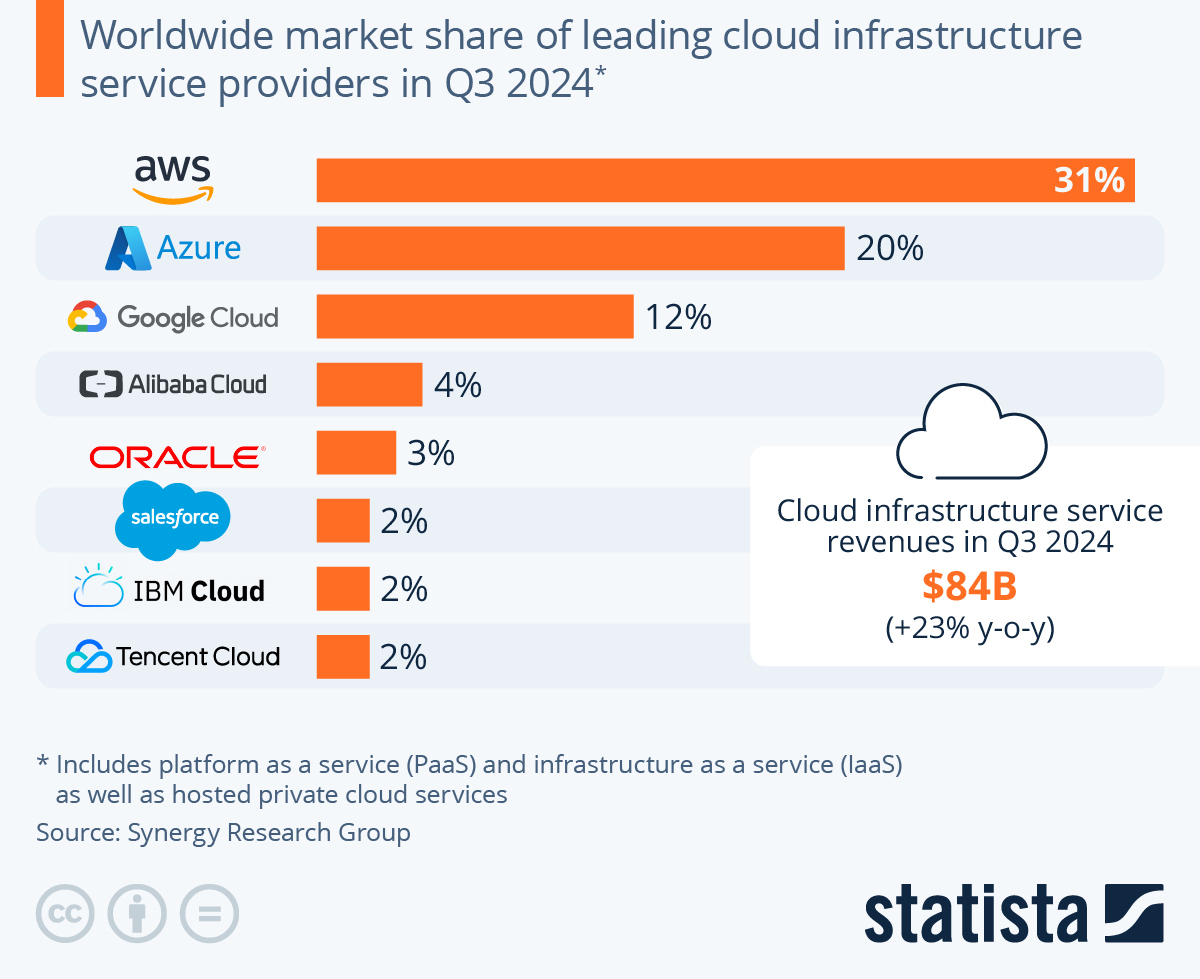
\includegraphics[width=0.75\linewidth]{images/pcp.jpeg}
    \caption{Worldwide market share of leading cloud infrastructure service providers as of Q3 2024 \cite{statista}}
    \label{fig:pcp}
\end{figure}
  
\subsection{Regions and Availability Zones}

cloud regions
Cloud providers usually further divide region into availability zones
For the purpuse of this work, we will consider the concept of \textbf{cloud region} as the primary unit of deployment of cloud resources.
Each Region supports a subset of the available instance types.
We could safely assume that our workload specs are quite standard and therefore can be scheduled on any cloud region.
As of late 2024, the three major cloud service providers have established extensive global infrastructures.
Table \ref{tab:cloud_regions_azs} shows the number of regions and availability zones (AZs) for each provider as of Q4 2024 - Q1 2025
\cite{statista_cloud_regions} \cite{aws_infrastructure}.
We must note that the number of regions and availability zones is constantly changing as cloud providers are expanding their global infrastructure

\begin{table}[H]
    \centering
    \begin{tabular}{|l|c|c|}
    \hline
    \textbf{Cloud Provider} & \textbf{Regions} & \textbf{Availability Zones} \\
    \hline
    Amazon Web Services (AWS) & 36 & 114 \\
    \hline
    Microsoft Azure & 33 & 93 \\
    \hline
    Google Cloud Platform (GCP) & 40 & 121 \\
    \hline
    \end{tabular}
    \caption{Number of Cloud Regions and Availability Zones by Provider as of 2024 \cite{stat}}
    \label{tab:cloud_regions_azs}
\end{table}

each provider has a different number of regions and zones and also different naming conventions
there is no standardization in the industry for this. 
for instance a region located in London is called eu-west-2 in AWS, uk-west in Azure and europe-west2 in GCP.
For what concerns the geo-distribution of cloud regions, Figure \ref{fig:azure_data_centers} shows the location of \textbf{Azure cloud data centers} around the world and the country Grid Carbon Intensity as reported by Electricity Maps (year 2024) \cite{electricity_maps}.
Data center coordinates are retrieved by an Azure CLI command dump \cite{azure_data_centers_information}.

\begin{figure}[htb]
    \centering
    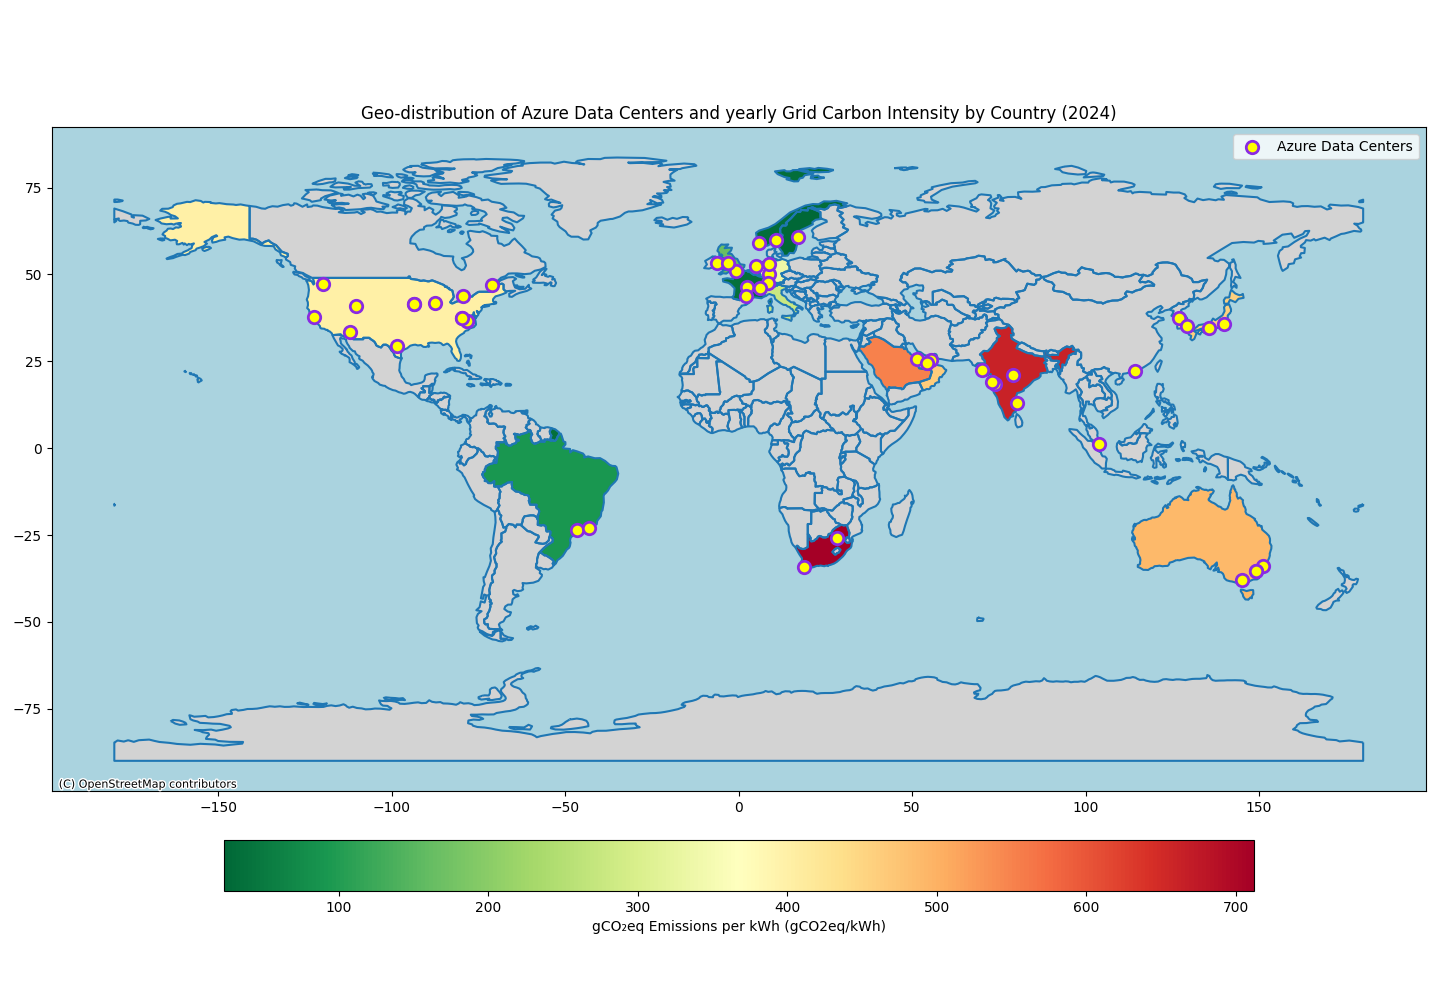
\includegraphics[width=1\linewidth]{images/azure_data_centers.png}
    \caption{Geo-distribution of Azure data centers with country Grid Carbon Intensity}
    \label{fig:azure_data_centers}
\end{figure}

% https://www.naturalearthdata.com/downloads/110m-cultural-vectors/


\subsection{Multi cloud paradigm}

what is multi cloud paradigm

why is useful
how to achieve

advantages of multi-cloud
flexibility
risk reduction (reduces vendor lock-in)

why it is important for the organizations


disadvantages
increased complexity
attack surface increased (security)




Why multi-cloud in the context of our system?
Different cloud providers have data centers in various locations around the world. This diversity allows for more options when geographically shifting workloads to regions with lower carbon intensity.
However the 3 big players have a big overlap: each one is present almost everywhere.
Multi-cloud paradigm could be leveraged for lowering costs.
For basic use cases, we can even set a single cloud provider to be used (e.g., Azure) and therefore just a multi-region environment.
Being able to work in a multi-cloud environment is also important for accomplishing user / company needs: they can use just a single cloud provider or more than one for different reasons. Therefore if our system supports more cloud providers, it will accomplish more users' needs.
If the system is designed to be multi-cloud then flexibility is higher for organizations and users.
For the purpose of this work, we will consider only the 3 major Public Cloud Provider as of today: AWS, Azure, GCP

\section{Kubernetes}

Kubernetes is an open-source platform for automating the orchestration of containerized applications.
It is widely used in the industry and became the \textbf{de-facto standard for container orchestration}.
An extensive description of Kubernetes is out of the scope of this thesis but it is deemed necessary to provide a brief overview of the main concepts of Kubernetes that are relevant for the purpose of this work.
Figure \ref{fig:kubernetes_architecture} shows the Kubernetes architecture as described by the Cloud Native Computing Foundation (CNCF) \cite{kubernetes_cnfc}.

\begin{figure}[htb]
    \centering
    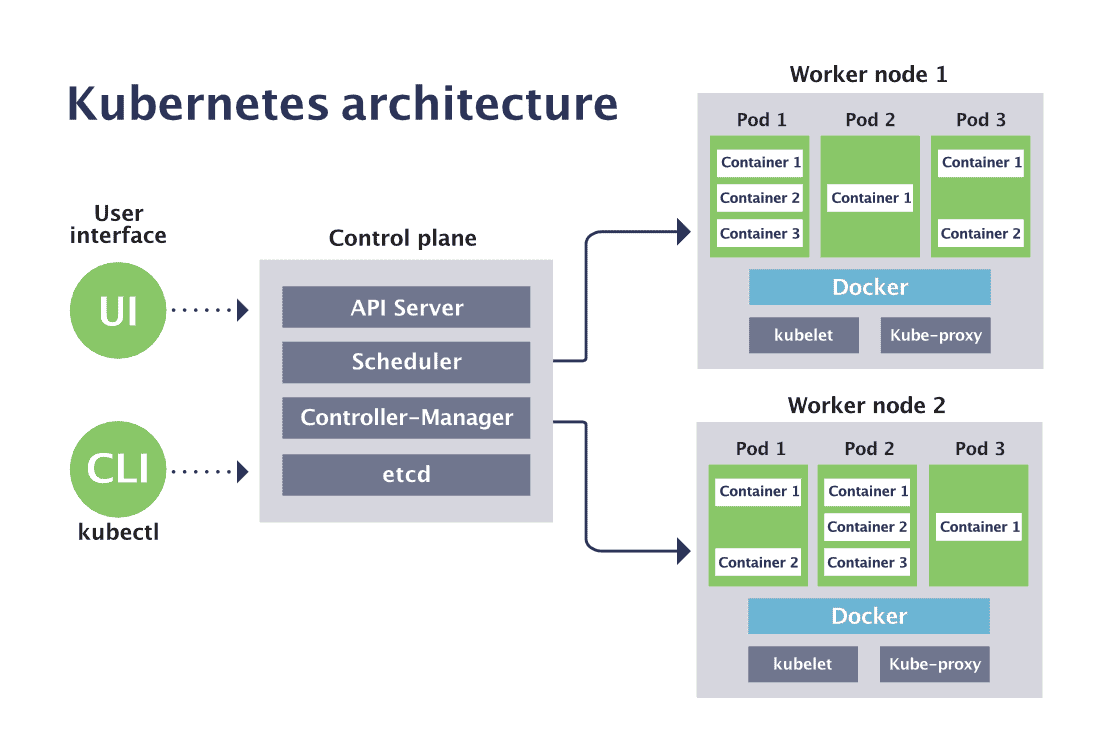
\includegraphics[width=1\linewidth]{images/kubernetes-architecture-diagram.png}
    \caption{Kubernetes architecture by CNCF \cite{kubernetes_cnfc}}
    \label{fig:kubernetes_architecture}
\end{figure}

The main components of Kubernetes are:
\begin{itemize}[itemsep=0.2pt, topsep=1pt]
    \item[$\bullet$] \textbf{Kubernetes API server}: the central component that manages the Kubernetes cluster. It exposes the Kubernetes API and is responsible for validating and mutating data related to Kubernetes objects.
    \item[$\bullet$] \textbf{etcd}: a key-value store used to store the cluster state.
    \item[$\bullet$] \textbf{Kubernetes controller manager}: a daemon that embeds the core control loops shipped with Kubernetes.
    \item[$\bullet$] \textbf{Kubernetes scheduler}: a component that assigns Pods to nodes.
    \item[$\bullet$] \textbf{Kubelet}: an agent that runs on each node in the cluster. It makes sure that containers are correctly running in a Pod.
    \item[$\bullet$] \textbf{Kubernetes proxy}: a network proxy that runs on each node in the cluster. It maintains network rules and it is responsible for routing network traffic.
    \item[$\bullet$] \textbf{Container runtime}: the software that is responsible for running containers on the Node (in this case represented by Docker).
\end{itemize}

It must be noted that in our system we are not extending the Kubernetes scheduler as described for instance in the works described in section \ref{sec:low_carbon_k8s_scheduler} and \ref{sec:microsoft_carbon_aware_k8s}, since we are not dealing with the scheduling of in-cluster resources (e.g., Kubernetes Pods) nor with the provisioning of entire Kubernetes clusters.
We are instead focusing on the \textbf{management of external resources on cloud providers} (only VMs in this first iteration), leveraging Kubernetes as a control plane for the management of these resources.
As described in the following section, our focus will be on the Kubernetes API server and in particular on Kubernetes Admission Control.

\subsection{Kubernetes extendability}

% https://www.cncf.io/blog/2022/06/15/kubernetes-operators-what-are-they-some-examples/

Kubernetes allows for the extension of its functionalities through the use of \textbf{Custom Resource Definitions (CRDs)} and \textbf{Kubernetes Operators}, effectively adopting the so-called \textbf{Operator paradigm}.
Simply put, Custom Resource Definitions are a way to instruct Kubernetes to manage new resource types. 
They are a \textbf{schema} that defines the structure of the resource and the Kubernetes API server will validate the resource against the schema.
\textbf{Custom Resources (CRs)} are actually instances of the resources defined by CRDs and are managed by an Operator.
The Operator is a piece of software (controller) that is responsible for managing the lifecycle of the resources defined by the CRD.
Effectively the code of an Operator is usually deployed on the Kubernetes cluster in the form of a Deployment.
This concept is not much different of what actually happens for standard built-in Kubernetes resources which are however manged by built-in controllers (e.g., Deployment controller, ReplicaSet controller, part of Kubernetes controller manager).
An high-level overview of the Operator paradigm is depicted in Figure \ref{fig:operator_paradigm}.

\begin{figure}[H]
    \centering
    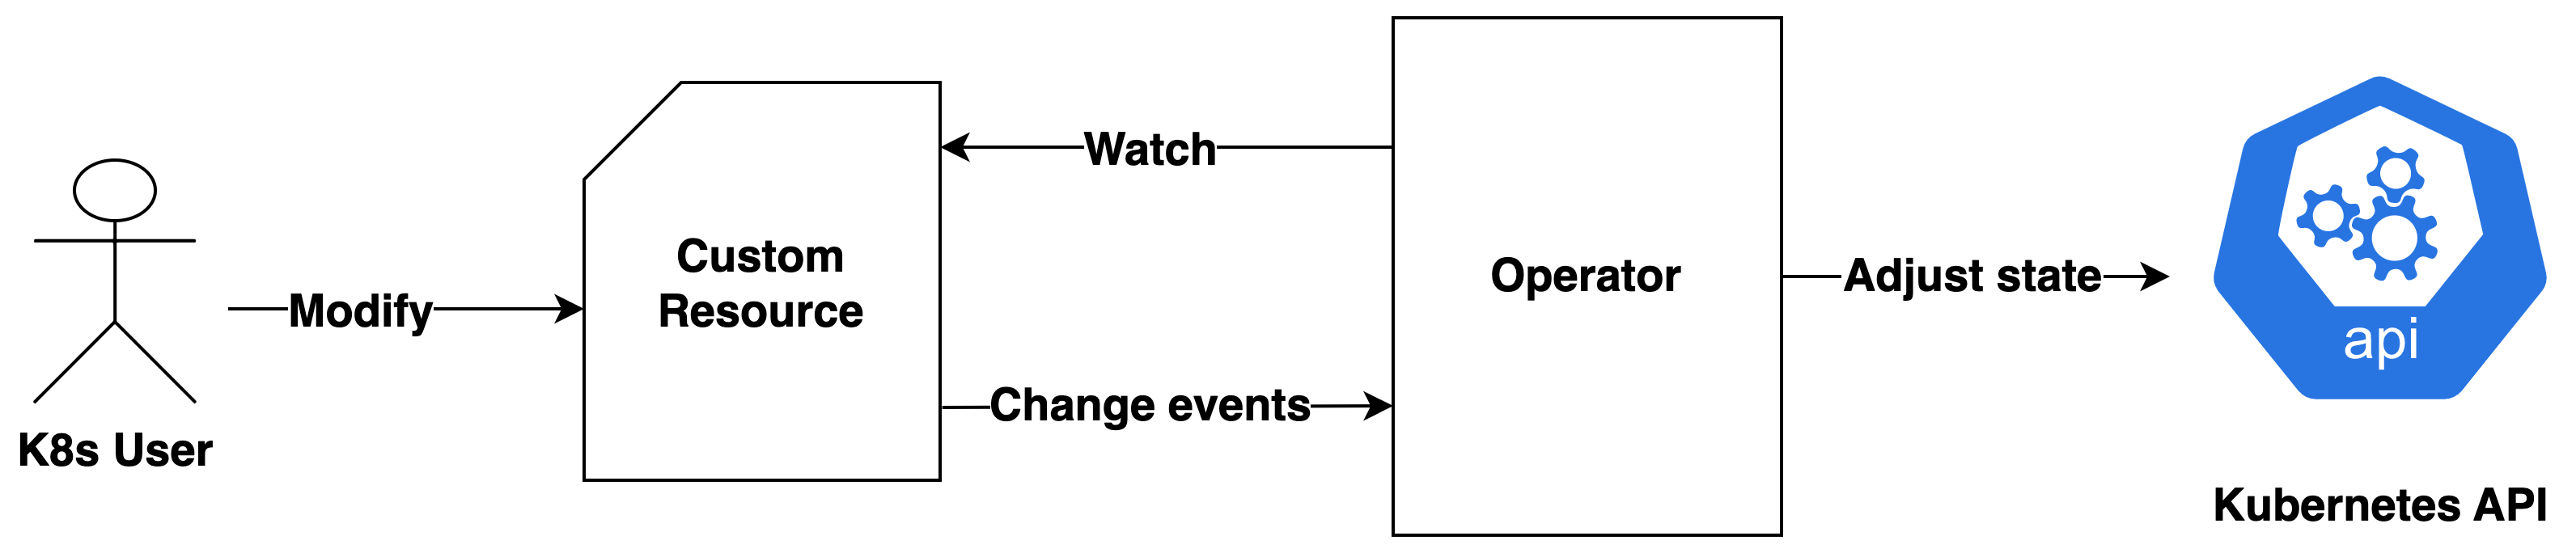
\includegraphics[width=1\linewidth]{images/opeartor_paradigm.png}
    \caption{Operator paradigm}
    \label{fig:operator_paradigm}
\end{figure}

\subsection{Kubernetes as a platform}

Recently, the paradigm of leveraging Kubernetes as a platform to manage external resources has become more and more popular.
Therefore, Kubernetes use cases have expanded beyond the management of containerized applications to the management of any desired resource on any infrastructure.
The idea is to \textbf{represent external resources as Kubernetes objects} and leverage Kubernetes' declarative paradigm and robust API to achieve unified and efficient infrastructure management.
This approach can be exemplified by the public cloud providers' operators which extend Kubernetes to manage their cloud resources as described in section \ref{sec:cloud_providers_operators}.

Config Connector is a Kubernetes operator developed by Google Cloud that allows to configure numerous Google Cloud services and resources using Kubernetes tooling and APIs \cite{gcp_config_connector}.
The idea general idea is that organizations might have to deal with a \textbf{heterogeneous infrastructure} composed of different cloud providers and on-premises resources. 
By \textbf{unifying infrastructure management under Kubernetes}, complexity is reduced and velocity is increased because the same tools and APIs can be used to manage all the resources in a consistent way \cite{gcp_config_connector}.


% https://aws.amazon.com/it/blogs/containers/kubernetes-as-a-platform-vs-kubernetes-as-an-api-2/


\subsection{Helm}

Helm is a \textbf{package manager} for Kubernetes. Therefore with Helm it is possible to define, install and manage Kubernetes applications in a simpler way compared to a manual management of Kubernetes resources manifests \cite{helm}.
Helm is a graduated project in the CNCF and it is the de-facto standard for Kubernetes package management.
The key concept is the \textbf{Helm chart}, which is a collection of files that describe a related set of Kubernetes resources. 
These files are mainly of two types: templates and values.
The \textbf{templates} are Kubernetes manifest files that are rendered by Helm's \textbf{powerful templating engine}. 
The \textbf{values} are the set of variables that are used to render the templates.
Upon an Helm chart installation, Helm will render the templates ``injecting" the values and deploy the resources in the Kubernetes cluster. 
One major advantage that Helm provides is the complete management of the lifecycle of the resources.
As a matter of fact, Helm allows to easily \textbf{upgrade}, \textbf{rollback} and \textbf{uninstall} the Kubernetes resources deployed with a Helm chart reducing time and errors in such operations \cite{helm}. 
Without Helm, the user would have to deal with each single Kubernetes resource manifest file and manually apply changes to them.
Finally, users can benefit of Helm charts already developed by the community and leverage chart distribution within their organization using Helm repositories.

\section{Krateo PlatformOps}
\label{sec:krateo}

Krateo PlatformOps (Krateo) is an \textbf{open-source Kubernetes-based platform} that aims to provide a unified interface for managing any desired resource on any infrastructure \cite{krateo_docs}.
Krateo runs as a Kubernetes deployment inside a Kubernetes cluster but \textbf{acts as a control plane} even for resource external to the Kubernetes cluster.
The only requirement for this management is that the resources need to be logically descriptible using a YAML file which represents the desired state of the resources \cite{krateo_docs}.
% Platform engineering
% Developer platform: a unified environment providing tools, services, and infrastructure that enables teams to efficiently build, test, and deploy software without managing underlying complexity. This complexity is handled by the platform team.
% Recognized by Gartner. Gartner said ... by 2025 companies without a ... (cite)
Krateo is composed of three main parts:
\begin{itemize}[itemsep=0.2pt, topsep=1pt]
    \item[$\bullet$] Krateo Composable Operations
    \item[$\bullet$] Krateo Composable Portal
    \item[$\bullet$] Krateo Composable FinOps
\end{itemize}

For the purpose of this work, we will focus on the \textbf{Krateo Composable Operations} part, which is the core of the Krateo platform and is responsible for managing the lifecycle of resources in a Kubernetes cluster \cite{krateo_docs}.
Krateo Composable Operations is composed in turn by several components. Due to their core importance in our system, as described in section XYZ we will briefly describe the functionalities of the \textbf{Krateo core-provider} and the \textbf{Krateo composition-dynamic-controller}.

\subsection{Krateo core-provider}

The Krateo core-provider is a Kubernetes operator that has the duty of downloading and managing Helm charts. It first checks for the existence of a file named \textit{values.schema.json} in the chart folder and uses it to generate a Kubernetes Custom Resource Definition (CRD), accurately representing the possible values that can be expressed for the installation of the chart \cite{krateo_core_provider}.
The file \textit{values.schema.json} is a JSON schema that describes the structure of the \textit{values.yaml} file for the related Helm chart and it is considered a standard best practice for Helm charts. It basically provides a way to validate the \textit{values}.yaml file before the Helm chart is installed (i.e., to check if the values are in the correct format).
In other words, the Krateo core-provider operator is responsible for deploying the Helm chart as a \textbf{native Kubernetes resource}, which allows for the management of the Helm chart lifecycle through Kubernetes APIs \cite{krateo_docs}.
As a matter of fact, out of the box, Kubernetes does not provide a way to manage Helm charts natively and the Krateo core-provider is one tool that allows to do so.
The Kubernetes Custom Resource Definition introduced by the Krateo core-provider is called \textbf{\textit{CompositionDefinition}}. It is a CRD that represents the Helm chart and its values (a Helm Chart archive (.tgz) with a JSON Schema for the values.yaml file) \cite{krateo_core_provider}.
Upon a CompositionDefinition manifest application to the Kubernetes cluster, the Krateo core-provider generates the CRD from the schema defined in the \textit{values.schema.json} file included in the chart. It then deploys an instance of the Krateo composition-dynamic-controller, setting it up to manage resources of the type defined by the CRD \cite{krateo_core_provider}.

\subsection{Krateo composition-dynamic-controller}

The Krateo composition-dynamic-controller is the Kubernetes operator that is instantiated by the Krateo core-provider to manage the Custom Resources whose Custom Resource Definition is generated by the core-provider.
In practice, when a Custom Resource (CR) is created, the instance of composition-dynamic-controller checks if a Helm release associated with the CR already exists in the cluster \cite{krateo_composition_dynamic_controller}. 
If this is not the case, it performs an \textit{helm install} operation using the values specified in the CR to create a new Helm release. This will practically deploy all the resources defined in the Helm chart using \textbf{Helm's templating engine}.
However, if the Helm release does already exist, it instead executes an \textit{helm upgrade} operation, updating the release's values with those specified in the CR, effectively updating the resources in the cluster.
Finally, when the CR is deleted from the cluster, the instance of the composition-dynamic-controller performs an \textit{helm uninstall} on the release, removing all the resources defined in the Helm chart from the cluster \cite{krateo_composition_dynamic_controller}. \\

The architecture of the Krateo core-provider and composition-dynamic-controller is depicted in Figure \ref{fig:krateo_core_provider}.

\begin{figure}[htb]
    \centering
    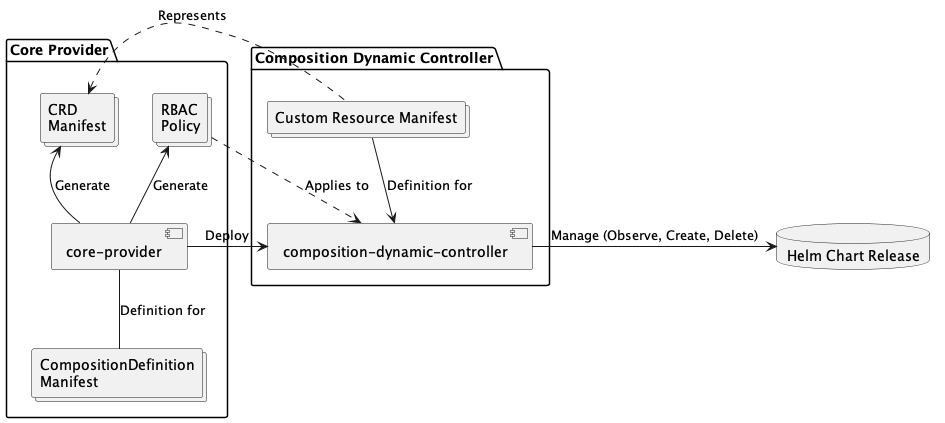
\includegraphics[width=1\linewidth]{images/kraeto_core_provider.png}
    \caption{Krateo core-provider and composition-dynamic-controller architecture \cite{krateo_core_provider}}
    \label{fig:krateo_core_provider}
\end{figure}

\section{Multi cloud resource management}
\label{sec:multi_cloud_resource_management}

The idea of a \textbf{dynamic management of workloads leveraging a multi-cloud paradigm} is not new. In this section we will provide an overview of some of the existing works in the literature that have tackled the problem of multi-cloud resource management.

\subsection{Dynamic Virtual Machine placement}
The work of Simarro et al. \cite{Simarro_2011} back at the dawn of cloud computing (2011) proposed a multi-cloud architecture for the dynamic placement of Virtual Machines (VMs).
The main objective of the system was cost optimization but this paradigm provides reliability and flexibility as well.
The scheduling part is comprised of a ``\textbf{cloud broker}" that is responsible for VM placement \textbf{transparent to users} providing a single uniform interface to the cloud resources.
Users can provide to the system a ``\textbf{service description template}'' to specify the number of VMs to provision and some constraints.
The cloud broker architecture is composed of two major components: the \textbf{scheduler} and the \textbf{cloud manager} \cite{Simarro_2011}. The former is responsible for placement decision across multiple cloud providers, while the latter is responsible for the actual management of the VMs in the cloud providers. More precisely, the cloud manager is represented by the OpenNebula (ONE) virtual infrastructure manager \cite{Simarro_2011}.
OpenNebula is an open-source platform that aims to provide a unified management interface for multiple virtualization technologies and cloud providers \cite{open_nebula}.

\subsection{Cloud service brokers}
A CSB is a system that acts as an \textbf{intermediary} between cloud service providers and consumers, providing a \textbf{unified interface} to manage cloud resources across multiple providers \cite{Wadhwa_2013}.
Cloud service brokers (CSBs) were described and categorized by Wadhwa et al. \cite{Wadhwa_2013} in their work of 2013.
The emerging market of cloud computing led to the proliferation of cloud services and providers, and by consequence the need for mechanisms to manage costs, capacity and resources \cite{Wadhwa_2013}. 
\newline

An interesting CSB example in the literature is the \textbf{STRATOS} system by Pawluk et al. proposed in 2012. The work can be considered a pioneer in the field of multi-cloud resource management since it can be framed in the first years of cloud computing \cite{STRATOS} but the proposed paradigms and concepts are relevant today.
STRATOS tried to \textbf{avoid the assumption of resource homogeneity} and represented an initial attempt to provide a ``\textbf{cross-cloud resource provisioning}'' system \cite{STRATOS}.
The proposed architecture enables the specification of high-level objectives that can be assessed in a standardized manner across different providers. The decision-making process is fully automated, shifting the decision point from deployment to runtime \cite{STRATOS}.
Users first submit a topology document, triggering the Cloud Manager to communicate with the Broker for topology instantiation. The Broker (implemented in Java) then conducts the initial resource acquisition decision (RAD), optimizing the allocation of resources across multiple providers (configured beforehand) \cite{STRATOS}.
Experiments indicate that distributing workloads across different cloud providers can reduce the overall cost of the topology. The approach taken by the authors primarily focuses on two objectives: \textbf{cost efficiency} and \textbf{avoiding vendor lock-in}. The application environment was deployed on public cloud platforms, specifically AWS and Rackspace \cite{STRATOS}.
\newline

[TO BE ADDED]
A Kubernetes 'Bridge' operator between cloud and external resources
% https://arxiv.org/abs/2207.02531

\subsection{AI-based resource management in cloud computing}
\label{sec:ai_based_resource_management}

More recent works have focused on the development of systems that leverage AI techniques for the optimization of resource management in cloud computing environments.

The work of 2022 by Khan et al. \cite{KHAN2022103405} provides a comprehensive review of the state of the art in the field of machine learning (ML)-centric resource management in cloud computing.
Although this works focuses on the cloud provider side (\textbf{resource management in data centers}), it provides some interesting insights that can be leveraged also at different levels of the cloud computing stack.
The authors highlight the fact that traditionally, only static policies were used for resource management in cloud computing, but the advent of ML techniques has enabled the development of more dynamic and adaptive resource management systems \cite{KHAN2022103405}. \newline
% maybe add some more insights from this work

Tuli et al. in their work of 2021 \cite{TULI2022111124} propose a system named \textbf{HUNTER} which stands for ``Holistic resoUrce
maNagemenT technique for Energy-efficient cloud computing using aRtificial intelligence''. 
In particular, in this work, tasks are modeled as \textbf{containers instances}.
For the purpose of this thesis, we can describe how this system was implemented from a infrastructural point of view.
The system is composed of four main components \cite{TULI2022111124}:
\begin{itemize}[itemsep=0.2pt, topsep=1pt]
    \item[$\bullet$] \textbf{Cloud Workload Management Portal}: a web-based portal that allows users to submit their workloads and specify the requirements (SLA constraints, QoS constraints, etc.).
    \item[$\bullet$] \textbf{Workload Manager}: a component that is responsible for the processing of incoming workloads.
    \item[$\bullet$] \textbf{Cloud Broker}:  the component that is responsible for the allocation of resources to cloud worker nodes
    \item[$\bullet$] \textbf{Cloud Hosts}: set of cloud worker nodes (in the form of both private and public cloud)
\end{itemize}
The Cloud Broker is the core of the system and is further divided into three sub-managers: Service Manager, CDC Manager, and Resource Manager.
The Service Manager is responsible for SLAs and QoS constraints, the CDC Manager is responsible for the actual allocation (provisioning) and migration of resources to cloud worker nodes and resource monitoring and the Resource Manager is responsible for the scheduling of tasks and contains the actual sustainability models (energy, thermal, cooling.) \cite{TULI2022111124}.

\subsection{Policy-driven resource management systems}

García García et al. (2014) propose \textbf{Cloudcompaas} \cite{GARCIAGARCIA20141}, a Service Level Agreement (SLA)-driven platform for dynamic cloud resource management, focusing on the automation of resource provisioning, scheduling, and monitoring
The aim of the work is to provide a SLA-aware Platform-as-a-Service platform for the entire management of cloud resource lifecycle \cite{GARCIAGARCIA20141}.
The targeted resource to be manages spans from IaaS to PaaS and SaaS.
Their approach leverage the WS-Agreement specification, a standard for SLA negotiation in web services, to define the SLA between the cloud provider and the cloud consumer \cite{GARCIAGARCIA20141}.
Leveraging this representation, they propose a SLA-driven architecture with three main components: the \textbf{SLA Manager}, the \textbf{Orchestrator}, and the \textbf{Infrastructure Connector} \cite{GARCIAGARCIA20141}.
The SLA Manager is the entry point for users and essentially builds and register agreements starting from the user requirements.
The Orchestrator, having a complete view of all the available cloud backends, performs the critical task of scheduling and resource allocation, considering the SLA constraints.
The Infrastructure Connector is the component that actually interacts with the cloud providers, performing the actual resource allocation and deallocation (provisioning and deprovisioning) \cite{GARCIAGARCIA20141}.
An interesting feature of the Infrastructure Connector is the ``configuration step'' in which arbitrary actions can be performed such as the \textbf{injection of a monitoring agent on a Virtual Machine}.
\newline

In the context of serverless computing environments, the work of 2021 by Mampage et al. \cite{9499407} proposes a deadline-aware dynamic resource management system.
The focus of the research is on both the provider and the consumer perspective, proposing a placement policy and ``dynamic resource management policy" that aims to minimize the cost of the provider while meeting the requirement of the consumer (i.e., the \textbf{deadline}) \cite{9499407}.
\newline


%[Policy-Based Cloud Management Through Resource Usage Prediction]
% https://link.springer.com/chapter/10.1007/978-3-319-13464-2_14

%---

% Optimizing Cost and Maximizing Profit for Multi-Cloud-Based Big Data Computing by Deadline-Aware Optimize Resource Allocation
% https://link.springer.com/chapter/10.1007/978-981-15-8469-5_3

\section{GreenOps landscape}

what is greenops

greenops landscape 

In the context of cloud-native sustainability,
the Technical Advisory Group (TAG) Environmental Sustainability is a XYZ that supports and advocates for environmental sustainability initiatives in cloud native technologies.

% https://hbr.org/2020/09/how-green-is-your-software

% https://www.usenix.org/publications/loginonline/slos-and-ghgs

\subsection{Green Software foundation}

The Green Software Foundation is a non-profit organization, part of the Linux Foundation, that aims to promote the development of green software and to provide a set of standards, tooling and best practices for the industry \cite{green_software_foundation}.
It is considered useful to provide a quick summary of the foundation's major projects that are relevant to the context of this work.

\subsubsection{Software Carbon Intensity Specification}

Software Carbon Intensity Specification (SCI) is a specification that aims to provide a standard way to measure the carbon intensity of software systems.
SCI is defined as a rate: the amount of carbon emissions per one unit of $R$ where $R$ is a functional unit for the software system (e.g., API call, new user, DB query, etc.) \cite{sci}.

The SCI can be defined as follows:
\[
SCI = C \times R = (O + M) \times R = ((E \times I) + M) \times R
\]

where:
\begin{itemize}[itemsep=0.2pt, topsep=1pt]
    \item[$\bullet$] $SCI$ is the Software Carbon Intensity
    \item[$\bullet$] $C$ is the carbon emissions
    \item[$\bullet$] $R$ is the functional unit
    \item[$\bullet$] $O$ is the operational emissions
    \item[$\bullet$] $M$ is the embodied emissions
    \item[$\bullet$] $E$ is the energy consumption
    \item[$\bullet$] $I$ is the carbon intensity
\end{itemize}

\subsubsection{Real Time Cloud}

The Real Time Cloud project aims to provide a standard for real-time carbon emissions data reporting for cloud providers.
The goal is to provide real-time access to information about cloud region, PUE, WUE, carbon-free energy from the grid and from CSP
The concept is similar to FOCUS specification for FinOps but is at a very early stage and is not yet adopted by cloud providers as of 2025 \cite{real_time_cloud}.

https://github.com/Green-Software-Foundation/real-time-cloud?tab=readme-ov-file

\subsubsection{Impact Framework}

The Impact Framework is a flexible framework for measuring and reporting the environmental impact of software systems \cite{impact_framework}.
The core of the framework is represented by a \textbf{Manifest file} which is a YAML file that is used both for describing \textbf{calculation pipelines} and for storing the results of the calculations.
Pre-built plugins are available for the most common calculations (e.g., carbon intensity, energy consumption, etc.) but custom plugins can be developed as well \cite{impact_framework}.
A potential integration of this framework with our system is described in section XYZ.

%---
%https://patterns.greensoftware.foundation/catalog/cloud/choose-region-closest-to-users
%[which patterns are used in our system]

\subsection{Computational Sustainability by Public cloud providers}

what are they already doing
improving energy efficiency by reducing their PUE
(Power Usage Effectiveness (PUE) is the ratio of the total energy used by a data center to the energy used for computing.)
---

We assume that a cloud data center will likely rely on the same energy sources that characterize a specific geographical region (grid).
For example, if data from Electricity Maps tell us that Finland is producing energy with low carbon emissions then we assume that the data centers in that area will likely be powered with energy from low carbon sources.
However, some cloud providers may have better access to renewable energy sources in certain regions due to their individual initiatives e.g. wind farms that feed directly into their data centers.


what microsoft is already doing with alternative energy sources apart from grid


---

Carbon aware computing at Google
https://www.performance2021.deib.polimi.it/www.performance2021.deib.polimi.it/wp-content/uploads/2021/11/Carbon-Aware-Computing-%40-Google-and-Beyond.pdf
Year: 2021
Description: 
It states that Carbon-aware computing is: exploiting flexibility in when and where and how computing is done to reduce carbon emissions.
Some examples of flexible workloads are: video processing, training large-scale machine learning models, simulation pipelines.
The components they recognized to be necessary are: accurate carbon intensity data (Tomorrow), Scalable infrastructures (Cloud), Virtualizations and migration mechanisms (VMs), Well identified flexible load, data-driven methodology.
At Google: the total amount of work that needs to get done per day is quite predictable.

https://blog.google/inside-google/infrastructure/data-centers-work-harder-sun-shines-wind-blows/

Google CFE\%: “This is the average percentage of carbon free energy consumed in a particular location on an hourly basis, while taking into account the investments we have made in carbon-free energy in that location. This means that in addition to the carbon free energy that's already supplied by the grid, we have added carbon-free energy generation in that location”.




usually big companies levarege financial instruments like PPAs to buy renewable energy therfore their emissions are not zero but they are offset by the renewable energy they buy.

\section{Carbon-aware systems for resource management}

Having provided an overview of the existing works in the field of multi-cloud resource management and having introduced the GreenOps landscape, we now focus on the state of the art in the field of carbon-aware resource management.
In particular, implementation choices and design patterns that can be leveraged for the development of a carbon-aware resource management system will be discussed.
\newline

The work of 2023 by Sukprasert et al. named ``\textit{Spatiotemporal Carbon-aware Scheduling in the Cloud: Limits and Benefits}'' \cite{10.1145/3599733.3606301} is a comprehensive analysis on the limits and benefits of the employment of geographical shifting and time shifting for cloud workloads.
The authors highlight the fact that different workloads have different characteristics and therefore different degrees of flexibility. Those include, for instance: \textbf{execution deadlines}, \textbf{data protection laws}, and \textbf{latency requirements}. Therefore, carbon savings are constrained by a complex set of factors that need to be taken into account when designing a carbon-aware system \cite{10.1145/3599733.3606301}.
The following sections will present systems that have been developed by various research groups to tackle the problem of carbon-aware resource management in cloud computing environments.

\subsection{CASPER}

CASPER (Carbon-Aware Scheduling and Provisioning for Distributed Web Services) is a carbon-aware scheduling and provisioning system whose primary purpose is to minimize the carbon footprint of distributed web services \cite{Souza_2023}.
The system is defined as a multi-objective optimization problem that considers two factors: the \textbf{variable carbon intensity} and the \textbf{latency constraints} of the network \cite{Souza_2023}.
By evaluating the framework in real-world scenarios, the authors demonstrate that CASPER achieves significant reductions in carbon emissions (up to 70\%) while meeting application \textbf{Service Level Objectives (SLOs)}, highlighting its potential for practical implementation in large-scale distributed systems \cite{Souza_2023}.
The authors of CASPER highlight the importance of considering the workload characteristics such as memory state, \textbf{latency} and \textbf{regulatory constraints such as GDPR} \cite{Souza_2023}.
The system is not adopting time-shifting since it is dealing with web services that are by their nature non-stopping workloads. The architecture is tied to scheduling K8s resources inside K8s clusters and does not consider external resource management.
%https://github.com/carbonfirst/casper?tab=readme-ov-file
%[HOW is it deployed]

\subsection{CASPIAN}

A research on carbon-aware scheduling in Kubernetes environments was conducted by the authors of CASPIAN (A Carbon-aware Workload Scheduler in Multi-Cluster Kubernetes Environments) \cite{10786568}.
The proposed system leverages Multi Cluster App Dispatcher (MCAD), a multi-cluster management platform, to provision workloads over distributed Kubernetes clusters \cite{10786568}.
Caspian is a scheduling and placement controller which lives in a master cluster and interacts with the MCAD to provision workloads across multiple geographical distributed clusters \cite{10786568}.
In particular, two main components are described: the \textbf{carbon tracker} and the \textbf{scheduler}.
The carbon tracker is responsible for the periodic collection of carbon intensity data along with worker cluster locations.
The scheduler, taking into account cluster information (carbon intensity, power efficiency, etc.), and workload requirements (e.g, \textbf{run time}, \textbf{deadline}, etc.), is responsible for the scheduling (time) and placement (geographical) of the workloads \cite{10786568}.

\subsection{CarbonScaler}

The work by Hanafy et al. ``\textit{CarbonScaler: Leveraging Cloud Workload Elasticity for Optimizing Carbon-Efficiency}" proposes a system that leverages the elasticity of batch cloud workloads to optimize carbon efficiency \cite{10.1145/3626788}.
The targeted workloads are for instance \textbf{MPI jobs} and \textbf{Machine Learning training jobs}.
The system is entirely Kubernetes-based and it is composed of three main components: the \textbf{Carbon Profiler}, the \textbf{Carbon AutoScaler}, and the \textbf{Carbon Advisor} \cite{10.1145/3626788}.
The Carbon Profiler main duty is to estimate energy usage of jobs.
The Carbon AutoScaler component is the core of the system and is a Kubernetes controller that leverage the \textbf{Kubeflow training operator}.
Kubeflow is effectively used for the resource management of batch jobs.
Finally, the Carbon Advisor simulates jobs execution in different configuration and allow the carbon reduction estimation \cite{10.1145/3626788}.

\subsection{A Low Carbon Kubernetes Scheduler}
\label{sec:low_carbon_k8s_scheduler}

The work is focused on the extension of the Kubernetes scheduler (``kube-scheduler'') for the ranking and filtering of the ``greenest'' region for the deployment of entire Kubernetes clusters \cite{low_carbon_k8s_scheduler}.
The system is tailored and tested on Azure but can be extended to other cloud providers.
Provisioning  operations of the clusters are done by the system leveraging Kubernetes API or IaaS management APIs \cite{low_carbon_k8s_scheduler}.
Therefore Kubernetes is leveraged as a control plane to provision other Kubernetes clusters.
An interesting feature proposed is the use of local air temperature and solar irradiance as tiebreaker for two datacenters with a similar carbon intense grid. 
The claim is that the solar irradiance has a bigger spread than the carbon intensity across global regions and that the local air temperature surrounding a datacentre affects the amount of energy needed for cooling \cite{low_carbon_k8s_scheduler}. 

\subsection{Microsoft's Carbon-Aware Kubernetes strategy}
\label{sec:microsoft_carbon_aware_k8s}

Citing to the previous work, Microsoft proposes a simple carbon-aware strategy for Kubernetes \cite{microsoft_carbon_aware_k8s}, integrating carbon intensity data into the scheduling process of Kubernetes Pods (rather than entire clusters).
The Kubernetes scheduler, which allows custom rules for assigning Nodes to Pods, can incorporate carbon metrics like the Marginal Operating Emissions Rate (MOER) as factors in placement decisions. 
A weighted distribution can be created by normalizing the MOER values across the available Nodes.
These weightings are encoded in a YAML file and applied as a priority for the Scheduler, which out-of-the-box supports these kind of custom rules to extend the scheduling process.
The claim is that by combining three elements (i.e., Kubernetes scheduler, carbon intensity data, and a weighting algorithm) any Kubernetes instance can be made carbon-aware, at least in a simplified way \cite{microsoft_carbon_aware_k8s}.

\section{State of the Art analysis outcome}




many simulation compared to real-world scenarios
no much flexibility for what concern variaty of resource managed
usually tied to one type of resource (e.g., VMs, K8s pods)

usually either time shifting or geographical shifting


Many of the concepts described in this chapter will be leveraged in the design and implementation of our system. 
We can list some of the recurrent elements that are generally needed in order to build a system for resource management
representation of a workload (with its characteristics and constraints)
cloud service broker / orchestrator
modules to directly interact with the cloud providers

\newpage

      \chapter{Design and Implementation}
\label{cha:design}

This chapter presents the design and implementation of our system, focusing on the integration of the various components and the overall architecture. The system is designed to be modular, scalable, and extensible, enabling the integration of additional components as needed.

\section{Assumptions}



\subsection{workload definition}
In this work, workload has been modeled as \textbf{Virtual Machines (VMs)}, representing the primary use case considered during the system's initial design phase. 
[WHY THIS CHOICE?]

We define, for the purpose of this work, a workload as a Virtual Machine (VM).
We can assume/imagine that inside of the VM, some kind of processing/work P will happen.
This VM can be scheduled on any Public Cloud Provider since we are looking for a multi-cloud setting: cloud can be seen as a commodity. 
Alternatively, a subset of eligible Public Cloud Providers can be set as a policy.
We can use general-purpose VMs.

The VM has the following characteristics:
MinCPU needed
MinRAM needed
Duration (D): the time duration that a VM must run to accomplish its processing/work
Deadline (DL): the time (timestamp) when the VM must have finish its work (maybe this can be omitted for the basic use cases)
Max latency (ML): value in ms 

If the workload is completely delay-tolerant then the Deadline parameter must not be used.

So a VM could be defined as a tuple like the following:
VM = (MinCPU, MinRAM, D, DL, ML)


example

Min CPU: 4 vCPU
Min RAM: 4 GB of RAM
Duration (D): 1h
Deadline (DL): 2022-12-31 23:59:59
---

The system is designed to be cloud-agnostic, however for the purpose of this work, the system is currently configured to support three major cloud providers: \textbf{Microsoft Azure}, \textbf{Google Cloud Platform (GCP)}, and \textbf{Amazon Web Services (AWS)}.

---






A limitation of our general approach is that only resources supported by the cloud provider’s Kubernetes operator can be provisioned. Not all cloud resources available in a provider’s portfolio are guaranteed to have corresponding Kubernetes Custom Resources (CRs). This introduces certain constraints:

\begin{itemize}[itemsep=0.2pt, topsep=1pt]
  \item[$\bullet$] Limited resource availability: if a specific resource type (e.g., a GPU-accelerated instance or a managed database service) is not supported by the cloud provider Operator, it cannot be provisioned using the current system.
  \item[$\bullet$] Dependence on Operator updates: cloud providers may extend or modify the set of resources supported by their Kubernetes operators over time.
  \item[$\bullet$] Vendor-specific implementations: different cloud providers expose varying levels of support for Kubernetes-native resource provisioning, leading to potential inconsistencies across multi-cloud environments.
\end{itemize}

Despite these constraints, the system architecture remains highly adaptable, and future enhancements could incorporate additional or alternative provisioning mechanisms. 
An example of an alternative implementation could be the direct API interactions with cloud providers to bypass operator limitations. Another approach could involve the development of custom operators or controllers to manage specific resource types not supported by existing operators. 
[KRATEO custom operator REST]

\newpage

\section{System Architecture}
\label{sec:system_architecture}

The following table provides an overview of the main components of the system and their respective functions.

\begin{table}[H]
  \centering
  \renewcommand{\arraystretch}{1.3} % Adjust row height for readability
  \begin{tabularx}{\textwidth}{| l | X |} % 'X' makes the second column auto-wrap
    \hline
    \textbf{Component} & \textbf{Function} \\
    \hline
    Krateo PlatformOps & Provides an abstraction layer for infrastructure orchestration, enabling declarative resource management and integration with cloud providers with templates. \\
    \hline
    Cloud Providers Kubernetes Operators & Manages the provisioning and reconciliation of cloud resources within Kubernetes, ensuring the actual state matches the desired state. \\
    \hline
    Kubernetes Mutating Webhook Configuration & Intercepts and modifies API requests before they are persisted, allowing dynamic configuration adjustments with policy enforcement. \\
    \hline
    OPA Server & Evaluates policy decisions based on defined constraints and input data from Kubernetes API requests through the webhook configuration. \\
    \hline
    OPA Policies and Data & Define the rules and contextual information used by OPA to make policy decisions, namely scheduling information \\
    \hline
    GreenOps Scheduler & Determines the optimal scheduling region and scheduling time for VMs, acting as an external data source for OPA policies. \\
    \hline
    MLflow & Allows the tracking, logging, versioning and storing of machine learning experiments for reproducibility and model lifecycle management. \\
    \hline
    KServe & Provides scalable and Kubernetes-native model serving capabilities, enabling deployment of machine learning models for inference. \\
    \hline
  \end{tabularx}
  \caption{Main components of the system and their respective functions.}
  \label{tab:system_components}
\end{table}

All the components listed in the above table must be deployed inside a Kubernetes cluster. The only exception are the OPA Policies and data which lies outside the cluster as described in section \ref{sec:opa_bundles}.

\section{Krateo PlatformOps integration}

Krateo PlatformOps is utilized in this system for \textbf{multi-cloud resource management}, allowing for the declarative orchestration of cloud resources across different cloud providers leveragin Kubernetes as a control plane. 
This section highlights the differences between two approaches for resource synchronization:
\begin{itemize}[itemsep=0.2pt, topsep=1pt]
  \item[$\bullet$] The \textbf{Custom Kubernetes ``Synchronization Operator"} approach
  \item[$\bullet$] The \textbf{Krateo PlatformOps} approach
\end{itemize}

It is deemed interesting to describe both approaches in order to identify the several trade-offs between implementing a custom synchronization operator and leveraging a template-based abstraction for cloud resource provisioning.

\subsection{Resource management: the Custom Kubernetes ``Synchronization Operator" approach}

When dealing with multi-cloud workloads with Kubernetes as a control plane, a synchronization and mapping mechanism (broker) is required to bridge the gap between:
\begin{itemize}[itemsep=0.2pt, topsep=1pt]
  \item[$\bullet$] \textbf{Generic Kubernetes Custom Resources}, which represent generic provider-agnostic workloads.
  \item[$\bullet$] \textbf{Cloud provider-specific Custom Resources}, which correspond to the actual cloud resources provisioned through the respective Kubernetes operators provided by Azure, AWS or GCP (in our case).
\end{itemize}

A custom Kubernetes Operator would be responsible for the mapping and synchronization of the above resource types. This approach is based on the principle of \textbf{Continuous Reconciliation}, where the operator continuously monitors and adjusts the system to maintain consistency between the desired and actual states.
Candidate solutions for the development of the K8s Operator includes: Operator SDK, Kubebuilder, or writing the operator from scratch using the Kubernetes client libraries. For the purpose of this work, Kubebuilder was used to develop a Proof of Concept (PoC) for the custom synchronization operator.

\subsubsection{Responsibilities of the Custom Operator}

In our specific case, the operator should continuously watch the generic CRs in the Kubernetes cluster to check if critical scheduling fields have been set:
\begin{itemize}[itemsep=0.2pt, topsep=1pt]
  \item[$\bullet$] \textbf{schedulingRegion}: Defines where the workload should be placed.
  \item[$\bullet$] \textbf{schedulingTime}: Specifies when the workload should be deployed.
\end{itemize}

These fields, if set, indicate a geographical placement and timing for the workload have been determined by the GreenOps Scheduler.
If these fields are not yet present, the operator must wait for scheduling decisions before proceeding.
Therefore, inside its Reconcile() loop, the operator should:
\begin{enumerate}[itemsep=0.2pt, topsep=1pt]
  \item Continuously check if scheduling fields (schedulingRegion, schedulingTime) are set.
  \item Trigger the creation of the provider-specific resource when the schedulingTime is approaching.
  \item Track the provisioning status by marking the generic CR with a field indicating that the cloud-specific resource has been created.
\end{enumerate}

\subsubsection{Post-Creation Considerations}

Once the cloud provider-specific resource is created, two main questions arise:
\begin{itemize}[itemsep=0.2pt, topsep=1pt]
  \item[$\bullet$] What happens if the provider-specific CR is modified manually?
  \item[$\bullet$] What happens if the VM configuration is modified directly on the cloud provider (outside Kubernetes)?
\end{itemize}

Related to the first question, an example scenario could be: changing the VM instance type (VM size) inside the Kubernetes cluster. In this case, the operator needs to decide whether to revert unauthorized changes or allow them and update the generic CR accordingly.
For the second question, an example could be: changing the VM size directly on the cloud provider’s console. In this case, the operator should detect the drift and update the generic CR to reflect the external changes.

\subsubsection{Resource linking}

A mechanism must be in place to link the generic CR to the cloud provider-specific CR. Possible approaches include:
\begin{itemize}[itemsep=0.2pt, topsep=1pt]
  \item[$\bullet$] UUID-based linking: A universally unique identifier ensuring each resource is mapped correctly.
  \item[$\bullet$] Kubernetes Object Metadata (ObjectMetadata.Name \& ObjectMetadata.Namespace): This approach may be preferable within a single Kubernetes cluster, avoiding the need for an external ID system.
\end{itemize}

\subsubsection{Termination Logic}

The operator must handle the deletion of cloud resources correctly in a variety of scenarios:
\begin{itemize}[itemsep=0.2pt, topsep=1pt]
  \item[$\bullet$] When the provider-specific CR is deleted from Kubernetes, the corresponding cloud resource is de-provisioned and the custom operator should ensure the deletion process is handled gracefully, avoiding orphaned generic CRs.
  \item[$\bullet$] If the provider-specific CR is deleted directly on the cloud provider, the operator should detect the change and update the generic CR accordingly.
  \item[$\bullet$] In the event of a generic CR deletion, the custom operator should ensure the provider specific resource is removed, troggering a deletion process on the cloud provider side (de-provisioning).
\end{itemize}

\subsubsection{Managing cloud provider-specific fields}
Each cloud provider has unique resource configurations and constraints that must be managed.
Some differences are purely syntactic (e.g., AWS uses instanceType, whereas Azure uses vmSize).
Others require additional provider-specific metadata (e.g., Azure requires a resourceGroup field which represent a logical container for resources in Azure).
A custom synchronization operator must encode this logic explicitly, making it more complex to maintain especially when supporting several cloud providers.

\subsubsection{Limitations of a Custom ``Synchronization Operator''}
Another major challenge with a custom synchronization operator is that some cloud providers do not support time scheduling metadata within their Custom Resources. In particular, no cloud operator among the ones we used for the system (AWS, Azure, GCP) provides a dedicated field for scheduling time.
This means that the Kubernetes operator itself must handle time scheduling logic, delaying CR creation until the scheduled time.
If the operator, upon the creation of a generic CR, immediately creates the cloud-provider specific CR (without a ``waiting logic''), the cloud provider Operator will trigger and provision the VM immediately, ignoring scheduling constraints.
Due to these limitations and complexities, we explored and leveraged an \textbf{alternative template-driven approach} using Krateo PlatformOps, described in the next section.

\begin{figure}[htb]
  \centering
  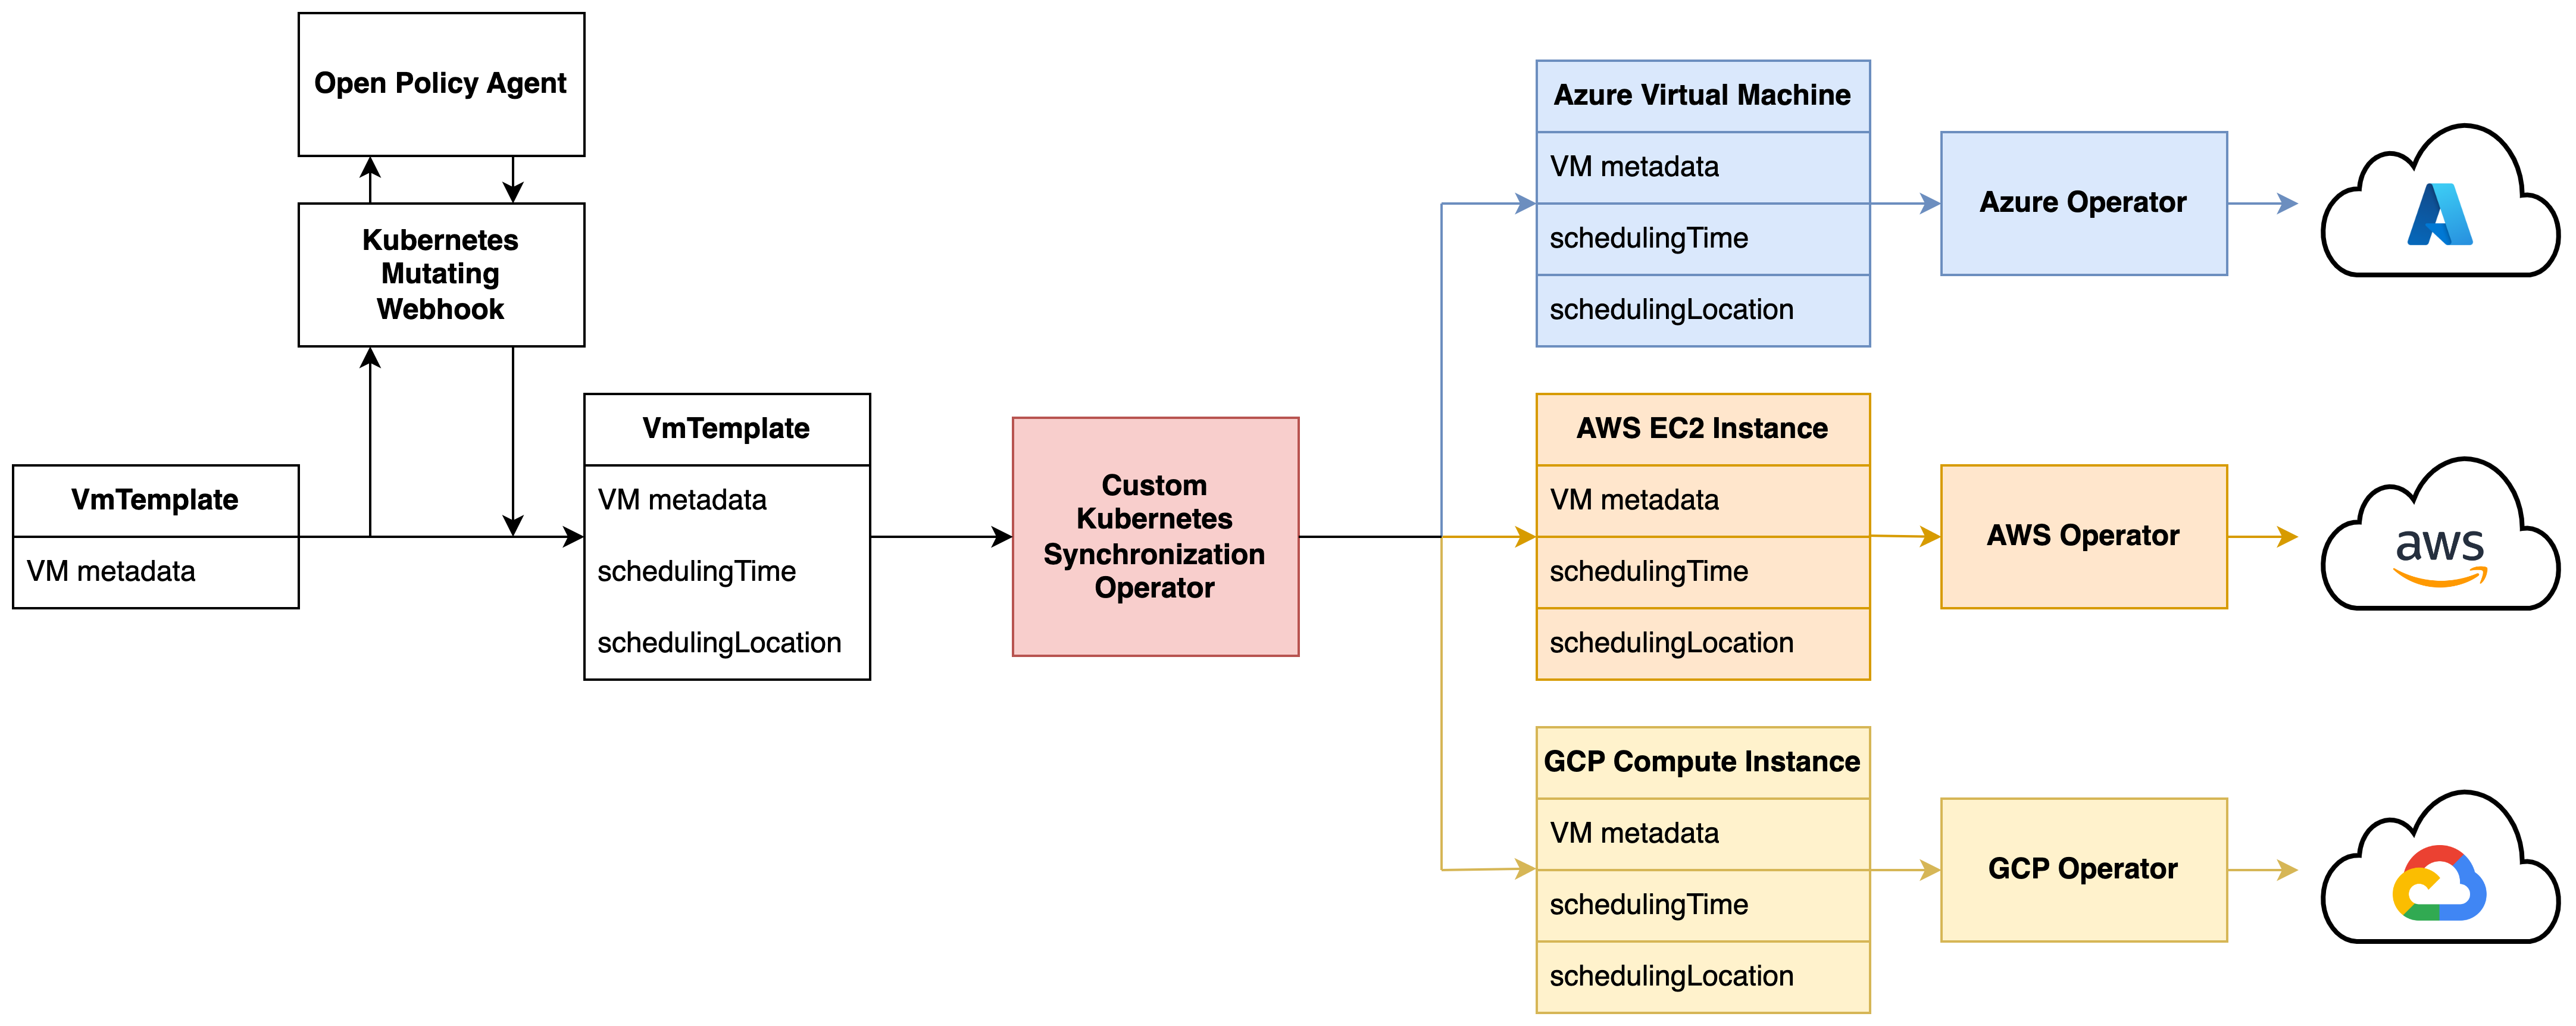
\includegraphics[width=1\linewidth]{images/k8s_operator.png}
  \caption{Multi-cloud resource management with Custom Kubernetes ``Synchronization Operator'' approach}
  \label{fig:k8s_operator}
\end{figure}

\subsection{Resource management: the Krateo approach}

\begin{figure}[htb]
  \centering
  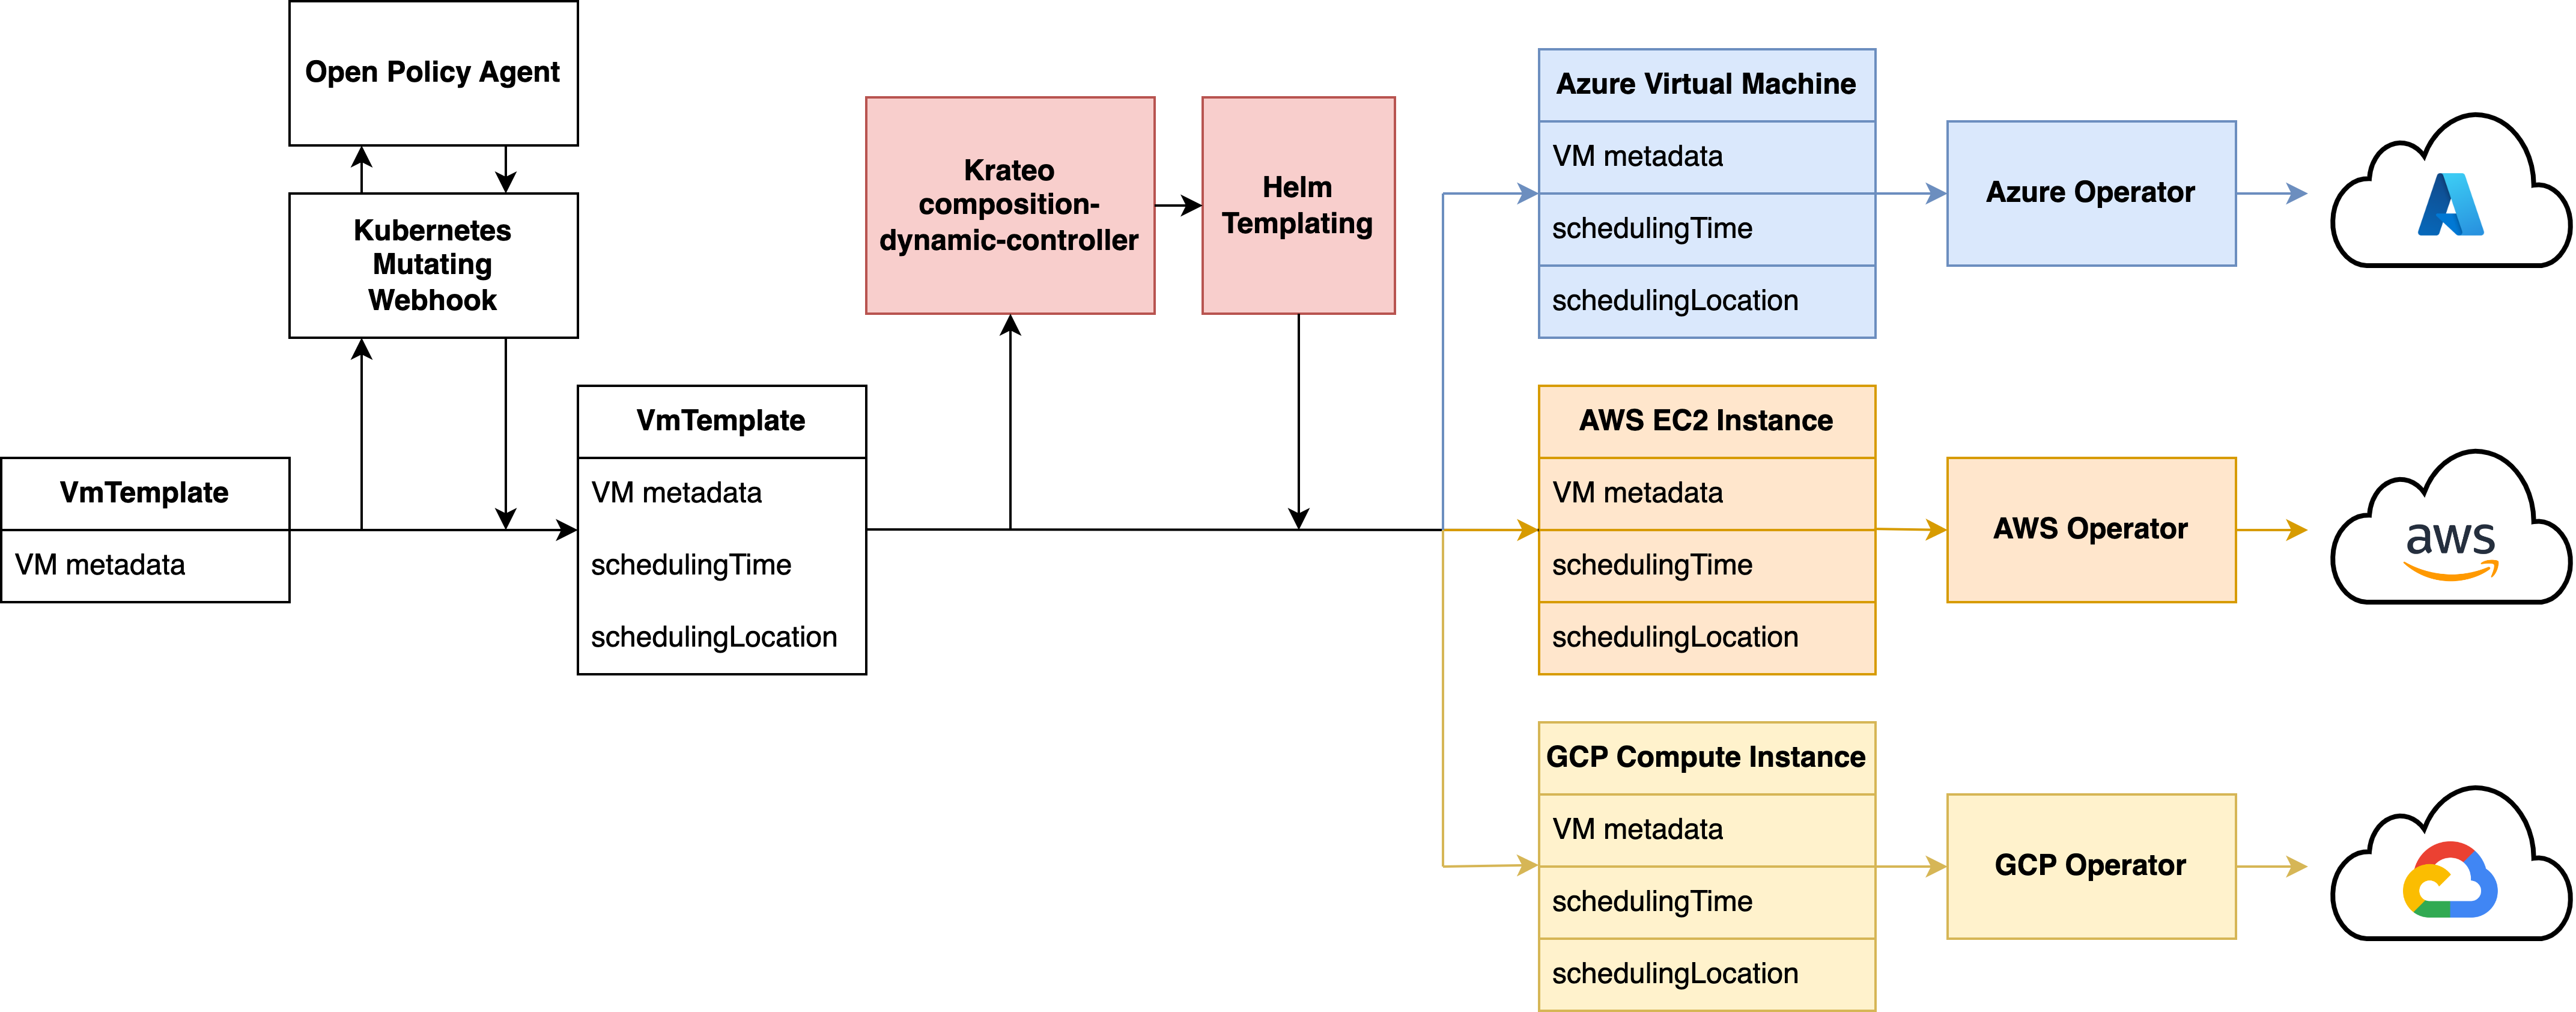
\includegraphics[width=1\linewidth]{images/krateo.png}
  \caption{Multi-cloud resource management with Krateo PlatformOps approach}
  \label{fig:krateo}
\end{figure}


krateo already described in section \ref{xyz}

Self-service platform for multi-cloud native resources

(generic VM mapped thanks to Krateo components, what is the added value)

generic workload resource definition
how to define it


\begin{lstlisting}[language=yaml, caption={values.yaml}, label={lst:values.yaml}]
# @param {string} vmName Name of the VM
vmName: test-vm

# @param {integer} cpu  Number of CPU cores
cpu: 1

# @param {integer} memory Number of GB of RAM
memory: 2

# @param {string} [schedulingTime] Scheduling Time for the VM
schedulingTime: 2025-05-05T00:00:00Z

# @param {string} [schedulingLocation] Scheduling Location for the VM
schedulingLocation: italynorth

# @param {string} duration Duration of the Workload
duration: 3h

# @param {string} deadline Deadline of the Workload
deadline: 2025-12-31T10:00:00Z

# @param {integer} maxLatency Maximum Latency of the Workload
maxLatency: 100
\end{lstlisting}


\lstset{style=jsonstyle}
\begin{lstlisting}[caption={values.schema.json}]
{
  "type": "object",
  "$schema": "http://json-schema.org/draft-07/schema",
  "required": [
    "vmName",
    "cpu",
    "memory",
    "duration",
    "deadline",
    "maxLatency"
  ],
  "properties": {
    "vmName": {
      "type": [
        "string"
      ],
      "description": "Name of the VM",
      "default": "test-vm"
    },
    "cpu": {
      "type": [
        "integer"
      ],
      "description": "Number of CPU cores",
      "default": "1"
    },
    "memory": {
      "type": [
        "integer"
      ],
      "description": "Number of GB of RAM",
      "default": "2"
    },
    "schedulingTime": {
      "type": [
        "string"
      ],
      "description": "Scheduling Time for the VM",
      "default": "2025-05-05T00:00:00Z"
    },
    "schedulingLocation": {
      "type": [
        "string"
      ],
      "description": "Scheduling Location for the VM",
      "default": "italynorth"
    },
    "duration": {
      "type": [
        "string"
      ],
      "description": "Duration of the Workload",
      "default": "3h"
    },
    "deadline": {
      "type": [
        "string"
      ],
      "description": "Deadline of the Workload",
      "default": "2025-12-31T10:00:00Z"
    },
    "maxLatency": {
      "type": [
        "integer"
      ],
      "description": "Maximum Latency of the Workload",
      "default": "100"
    }
  }
}
  
\end{lstlisting}


Helm template engine (how to map to cloud provider specific resources, why is better)


Multi-cloud VMs list and mapping
We need to know which VMs (instance types) are actually available on Azure, AWS, GCP.
What to actually use to fetch the list and where to store it
How frequent the elements changes and how to update the list (this is done with policy updates (updates to contextual data))
How to match generic workload to candidate VMs instance types (that adhere to the generic workload specs), what is the mapping logic.
For example:
Requested VM (generic): (2 vCPU, 16 GiB)
Chosen VM instance: Azure Standard E2as v4
What are the steps of the process to identify the correct VM instance?

Use Cloud Providers API / CLI and store the records in a local DB. Regular scheduled updates.
For our PoC we could maybe use a small subset of all the available instance types.

Current approach:
Map (CPU, RAM) => InstanceType

This mapping is done through Helm templating when creating 

compostion definition


krateo cdc
The composition-dynamic-controller is an operator that is instantiated by the core-provider to manage the Custom Resources whose Custom Resource Definition is generated by the core-provider.

\section{Kubernetes Mutating Webhook Configuration}

\subsection{Kubernetes Admission Control}

In the context of \textbf{Kubernetes Admission Control}, in addition to standard, compiled-in admission plugins, Kubernetes supports the use of additional admission plugins that are effectively extensions of the system and run as \textbf{webhooks} configured at runtime \cite{kubernetes_dynamic_admission_control}. This means that the admission control logic can be extended dynamically without the need to recompile the Kubernetes API server or other Kubernetes components. Changes are applied at runtime to the running Kubernetes cluster, making the system more flexible and adaptable.











These plugins can be used to enforce custom policies and perform additional validation and mutation of Kubernetes objects before they are persisted in the cluster.

K8s mutating webhook is used to modify K8s custom resources with the data from policies. 
The K8s mutating webhook intercepts the CREATE or UPDATE API request, asks about policies (with also scheduling decision) and mutates the resource.

we can distinguish between two types of webhooks: validating and mutating.

we can distinguish two entities semantically different: the webhook configuration and the actual webhook /server which perform mutation or validation

it could be a server that you need to implement to perform your own custum mutation or validation logic
it could be a service ready to use out of the box like OPA server

\begin{figure}[htb]
  \centering
  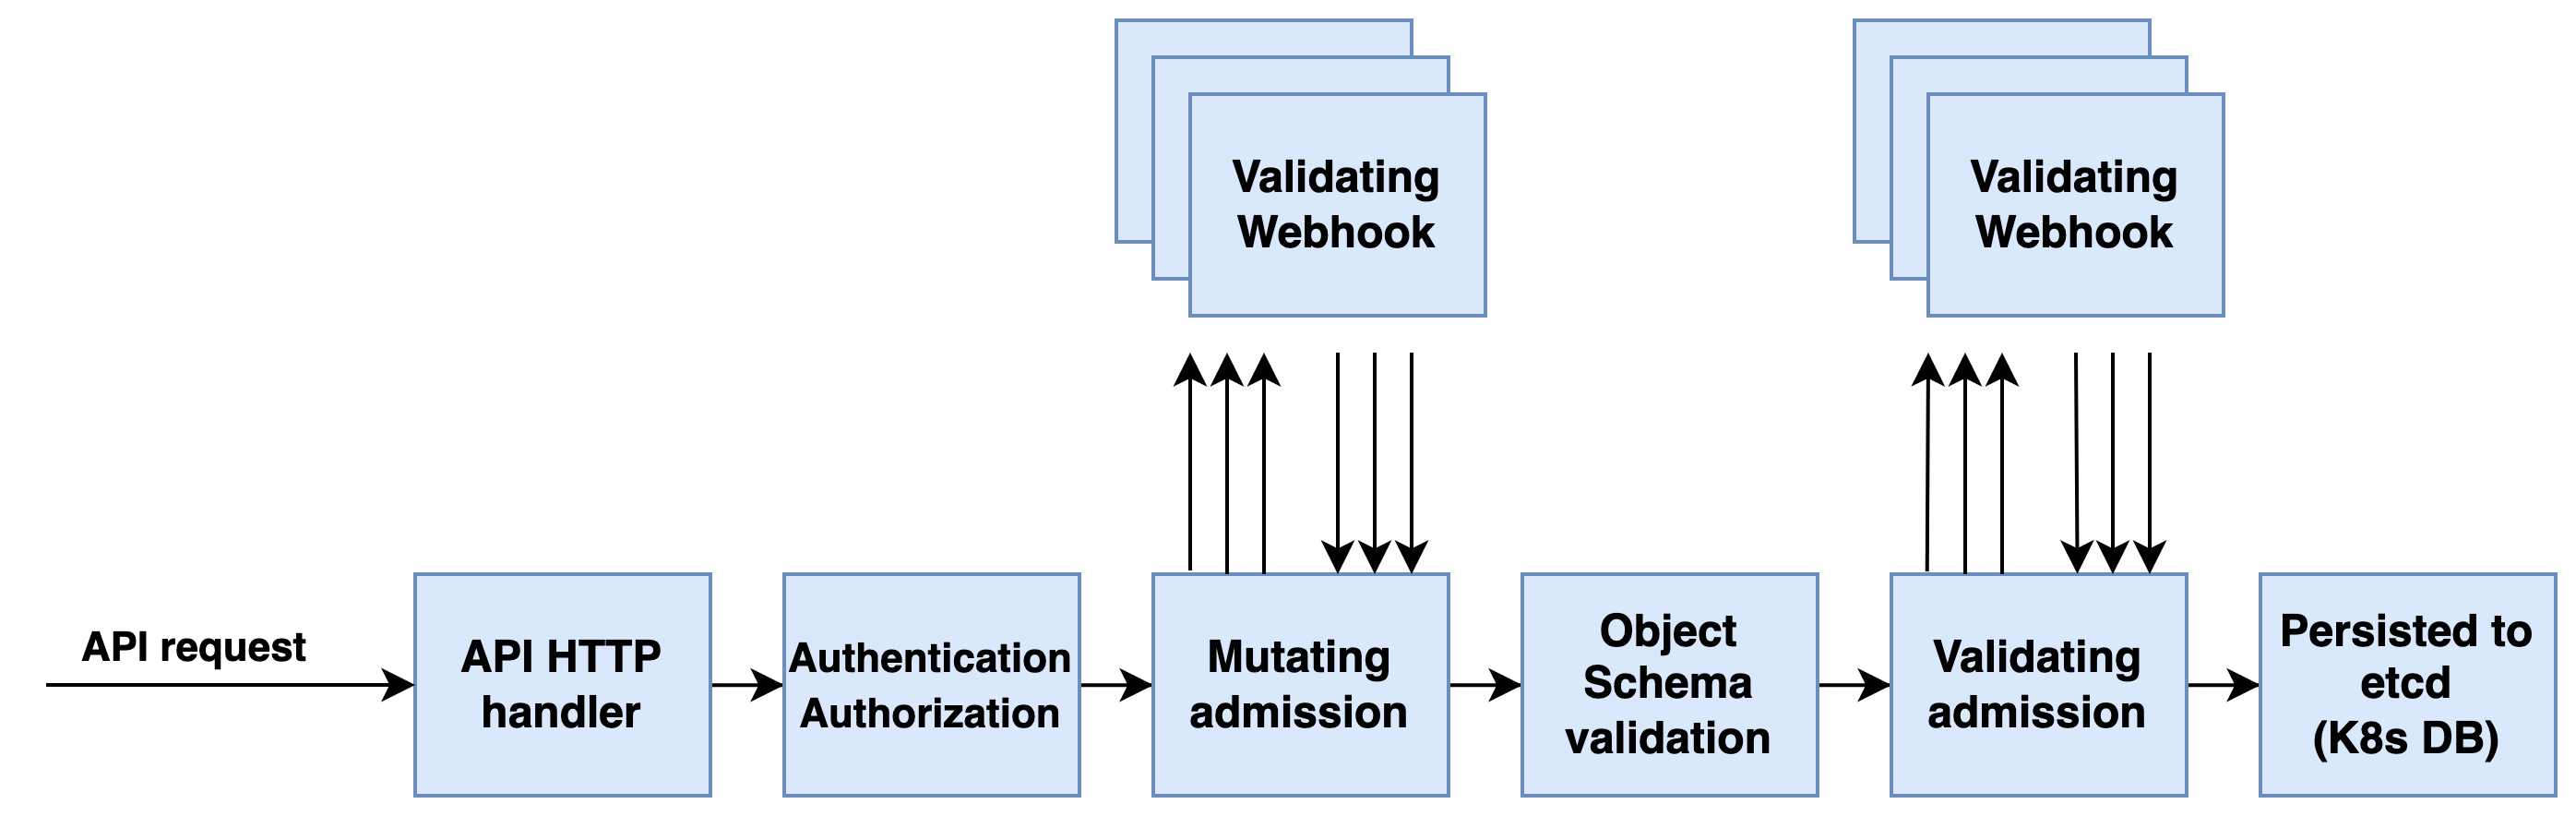
\includegraphics[width=1\linewidth]{images/k8s_admission.png}
  \caption{Kubernetes Admission Control}
  \label{fig:k8s_admission_control}
\end{figure}


service can be either a deployment with the related service inside the cluster like seen in the image \ref{fig:k8s_webhook_example}

or can be deployed outside the cluster

Figure \ref{fig:k8s_webhook_example} shows an example of a Kubernetes Mutating Webhook. The webhook server is deployed as a Kubernetes Deployment (with 1 Pod), with a corresponding Service to expose it within the cluster. The webhook server is responsible for receiving The AdmissionReview Request, applying custom logic, and returning an AdmissionReview Response to the Kubernetes API server describing the mutation to be applied to the resource.
The custom logic in this simple example is just to add a label "mutated: true" to the resource.

\begin{figure}[htb]
  \centering
  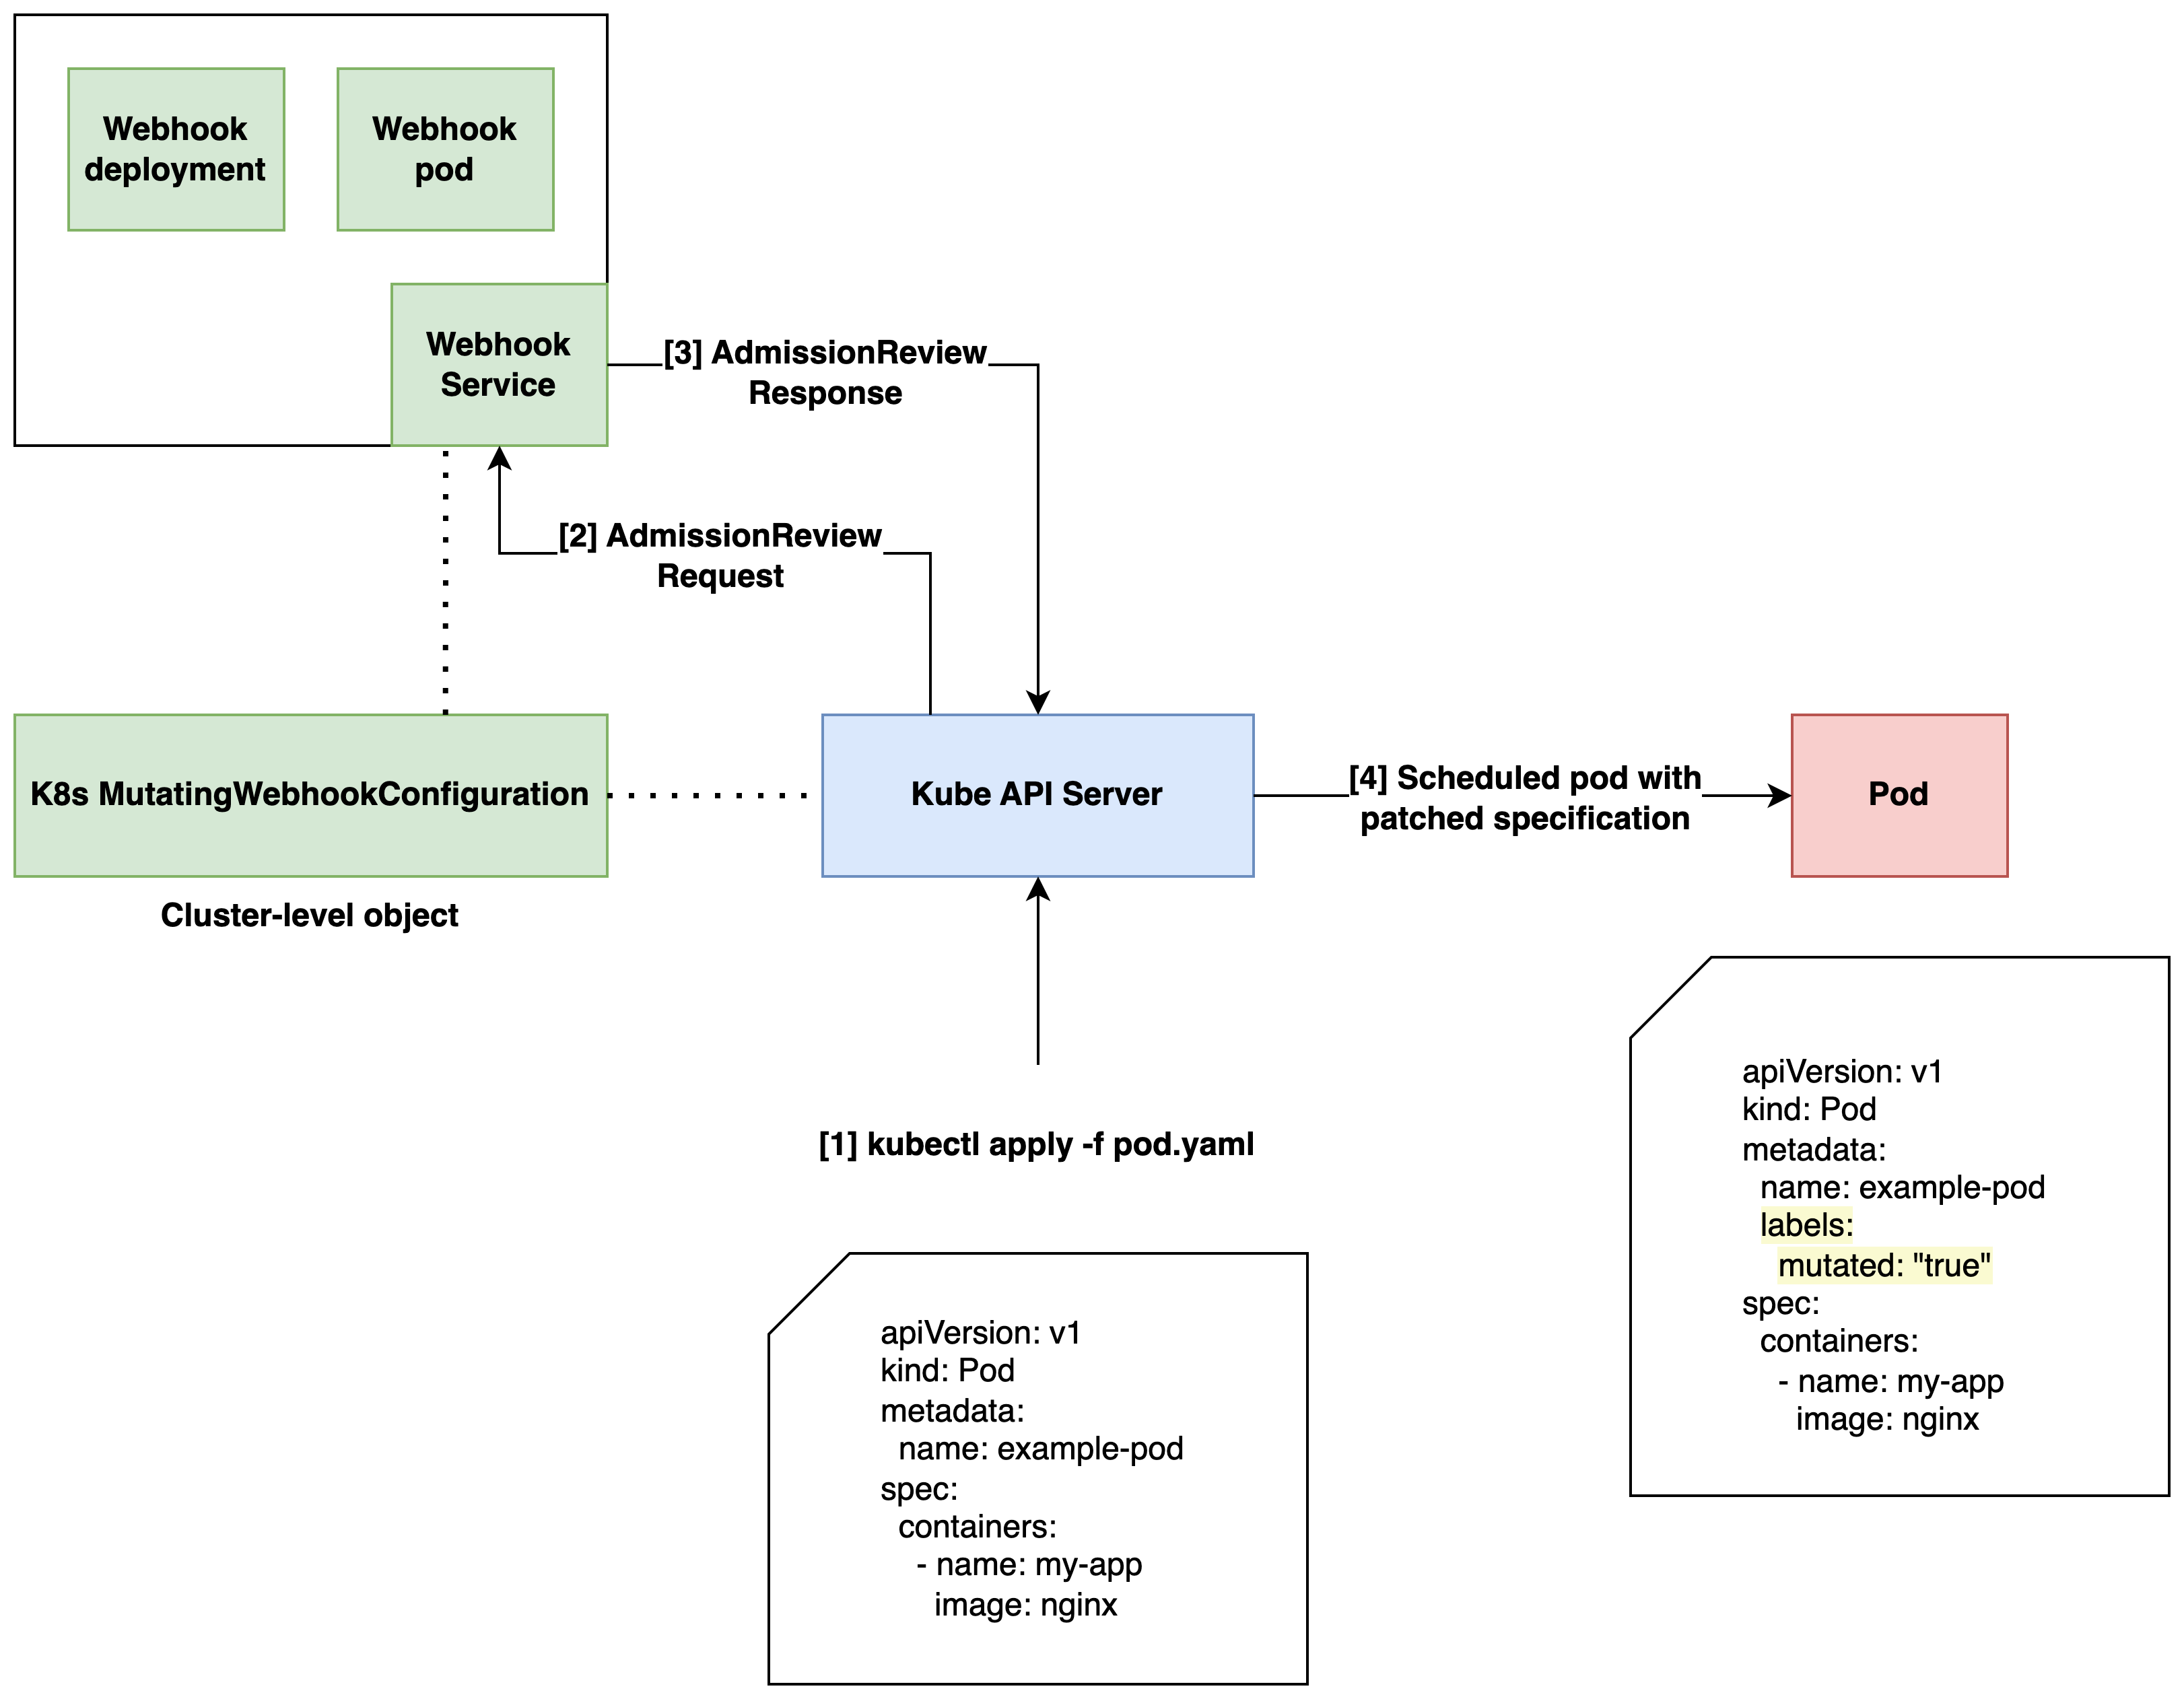
\includegraphics[width=1\linewidth]{images/k8s_webhook_example.png}
  \caption{Kubernetes Mutating Webhook example \cite{kubernetes_mutating_webhook_example}}
  \label{fig:k8s_webhook_example}
\end{figure}

\section{Multi-Cloud Integration through Kubernetes Operators}

The integration of operators from different cloud providers has enabled the development of an effective \textbf{multi-cloud system}, allowing seamless orchestration and provisioning of cloud resources across various cloud platforms. Namely, the system leverages Kubernetes operators from \textbf{Microsoft Azure}, \textbf{Google Cloud Platform (GCP)}, and \textbf{Amazon Web Services (AWS)}.

\subsection{Role of Kubernetes Operators}

Kubernetes operators work on the principle of Continuous Reconciliation, ensuring, in this case, that the desired state of the system, as defined by users, aligns with the actual state of provisioned cloud resources. In particular, Operators act as controllers that monitor, adjust, and manage external cloud resources within a Kubernetes-native environment. Inside the K8s lie the representation of the cloud resources, which are managed by the operators.
Key characteristics of operators include:
\begin{itemize}[itemsep=0.2pt, topsep=1pt]
  \item[$\bullet$] Managing external cloud resources within a Kubernetes cluster, providing a \textbf{unified interface} for multi-cloud deployments.
  \item[$\bullet$] Maintaining a \textbf{real-time representation} of provisioned cloud resources within Kubernetes.
  \item[$\bullet$] Using Custom Resources (CRs) to define cloud-specific resources in a \textbf{declarative} manner.
\end{itemize}

\subsection{Strategic Shift: From Custom Operator to Krateo Core Provider}

In our approach, we opted to replace a custom Kubernetes operator (``Synchronization Operator''), originally designed to handle the \textbf{mapping} from generic to cloud-specific resources, with \textbf{Krateo Core Provider}. This decision was motivated by the need for greater flexibility and maintainability in defining multi-cloud infrastructure components. As a matter of fact, the custom operator was originally designed to handle only virtual machines (VMs) mappings and extensions to support additional cloud resources would have required significant code changes and maintenance overhead for each additional resource type added.

Therefore instead of embedding business logic directly within a custom Kubernetes operator, in the current system implementation, we leverage the capabilities of \textbf{Helm templating} to dynamically generate cloud-provider-specific resources. More precisely, another Krateo component, the \textbf{Krateo composition-dynamic-controller} is leveraging Helm templating under the hood to generate Kubernetes resources starting from helm templates.
This approach, further described in the following sections, offers several advantages:

Simplified resource management:  Helm enables a standardized way define resources without maintaining complex operator logic.
Greater extensibility:  By externalizing the logic from the operator, future modifications and integrations with additional cloud providers become easier.
Reduced maintenance overhead: Operators typically require constant updates and refinements, while Helm-based resource generation minimizes the need for frequent code changes.

It must be noted that different cloud provider adopts different design choices for their Kubernetes operators and more in general for their overall infrastructure management. Therefore, for the creation of logically similar resources, like a virtual machine, the structure and the field of the resources can be different. 
These resources typically include:
\begin{itemize}[itemsep=0.2pt, topsep=1pt]
  \item[$\bullet$] Compute resources (e.g., VM instances, virtual machine templates)
  \item[$\bullet$] Networking components (e.g., virtual networks, subnets, security groups)
  \item[$\bullet$] Storage allocations (e.g., persistent volumes, cloud disks)
  \item[$\bullet$] Access management (e.g., resource groups, roles, authentication credentials)
\end{itemize}


For the purpose of this work we defined baseline infrastructure for each cloud provider in order to have a common ground for the system to work. This baseline infrastructure is composed by the minimum set of resources needed for a VM provisioning.

each providers has its complexities and nuances

vendor lock-in.





\newpage

\subsection{Azure Kubernetes Operator}

Microsoft Azure provides a Kubernetes operator called \textbf{Azure Service Operator v2} (ASO).
Currently, ASO supports more than 150 different Azure resources.
minimum set of resources needed for vm provisioning on Azure throgh Azure service operator is is:

\begin{itemize}[itemsep=0.2pt, topsep=1pt] \item[$\bullet$] Virtual Network 
\item[$\bullet$] Virtual Network Subnet
\item[$\bullet$] Network Interface
\item[$\bullet$] Virtual Machine
\end{itemize}

\begin{figure}[H]
\centering
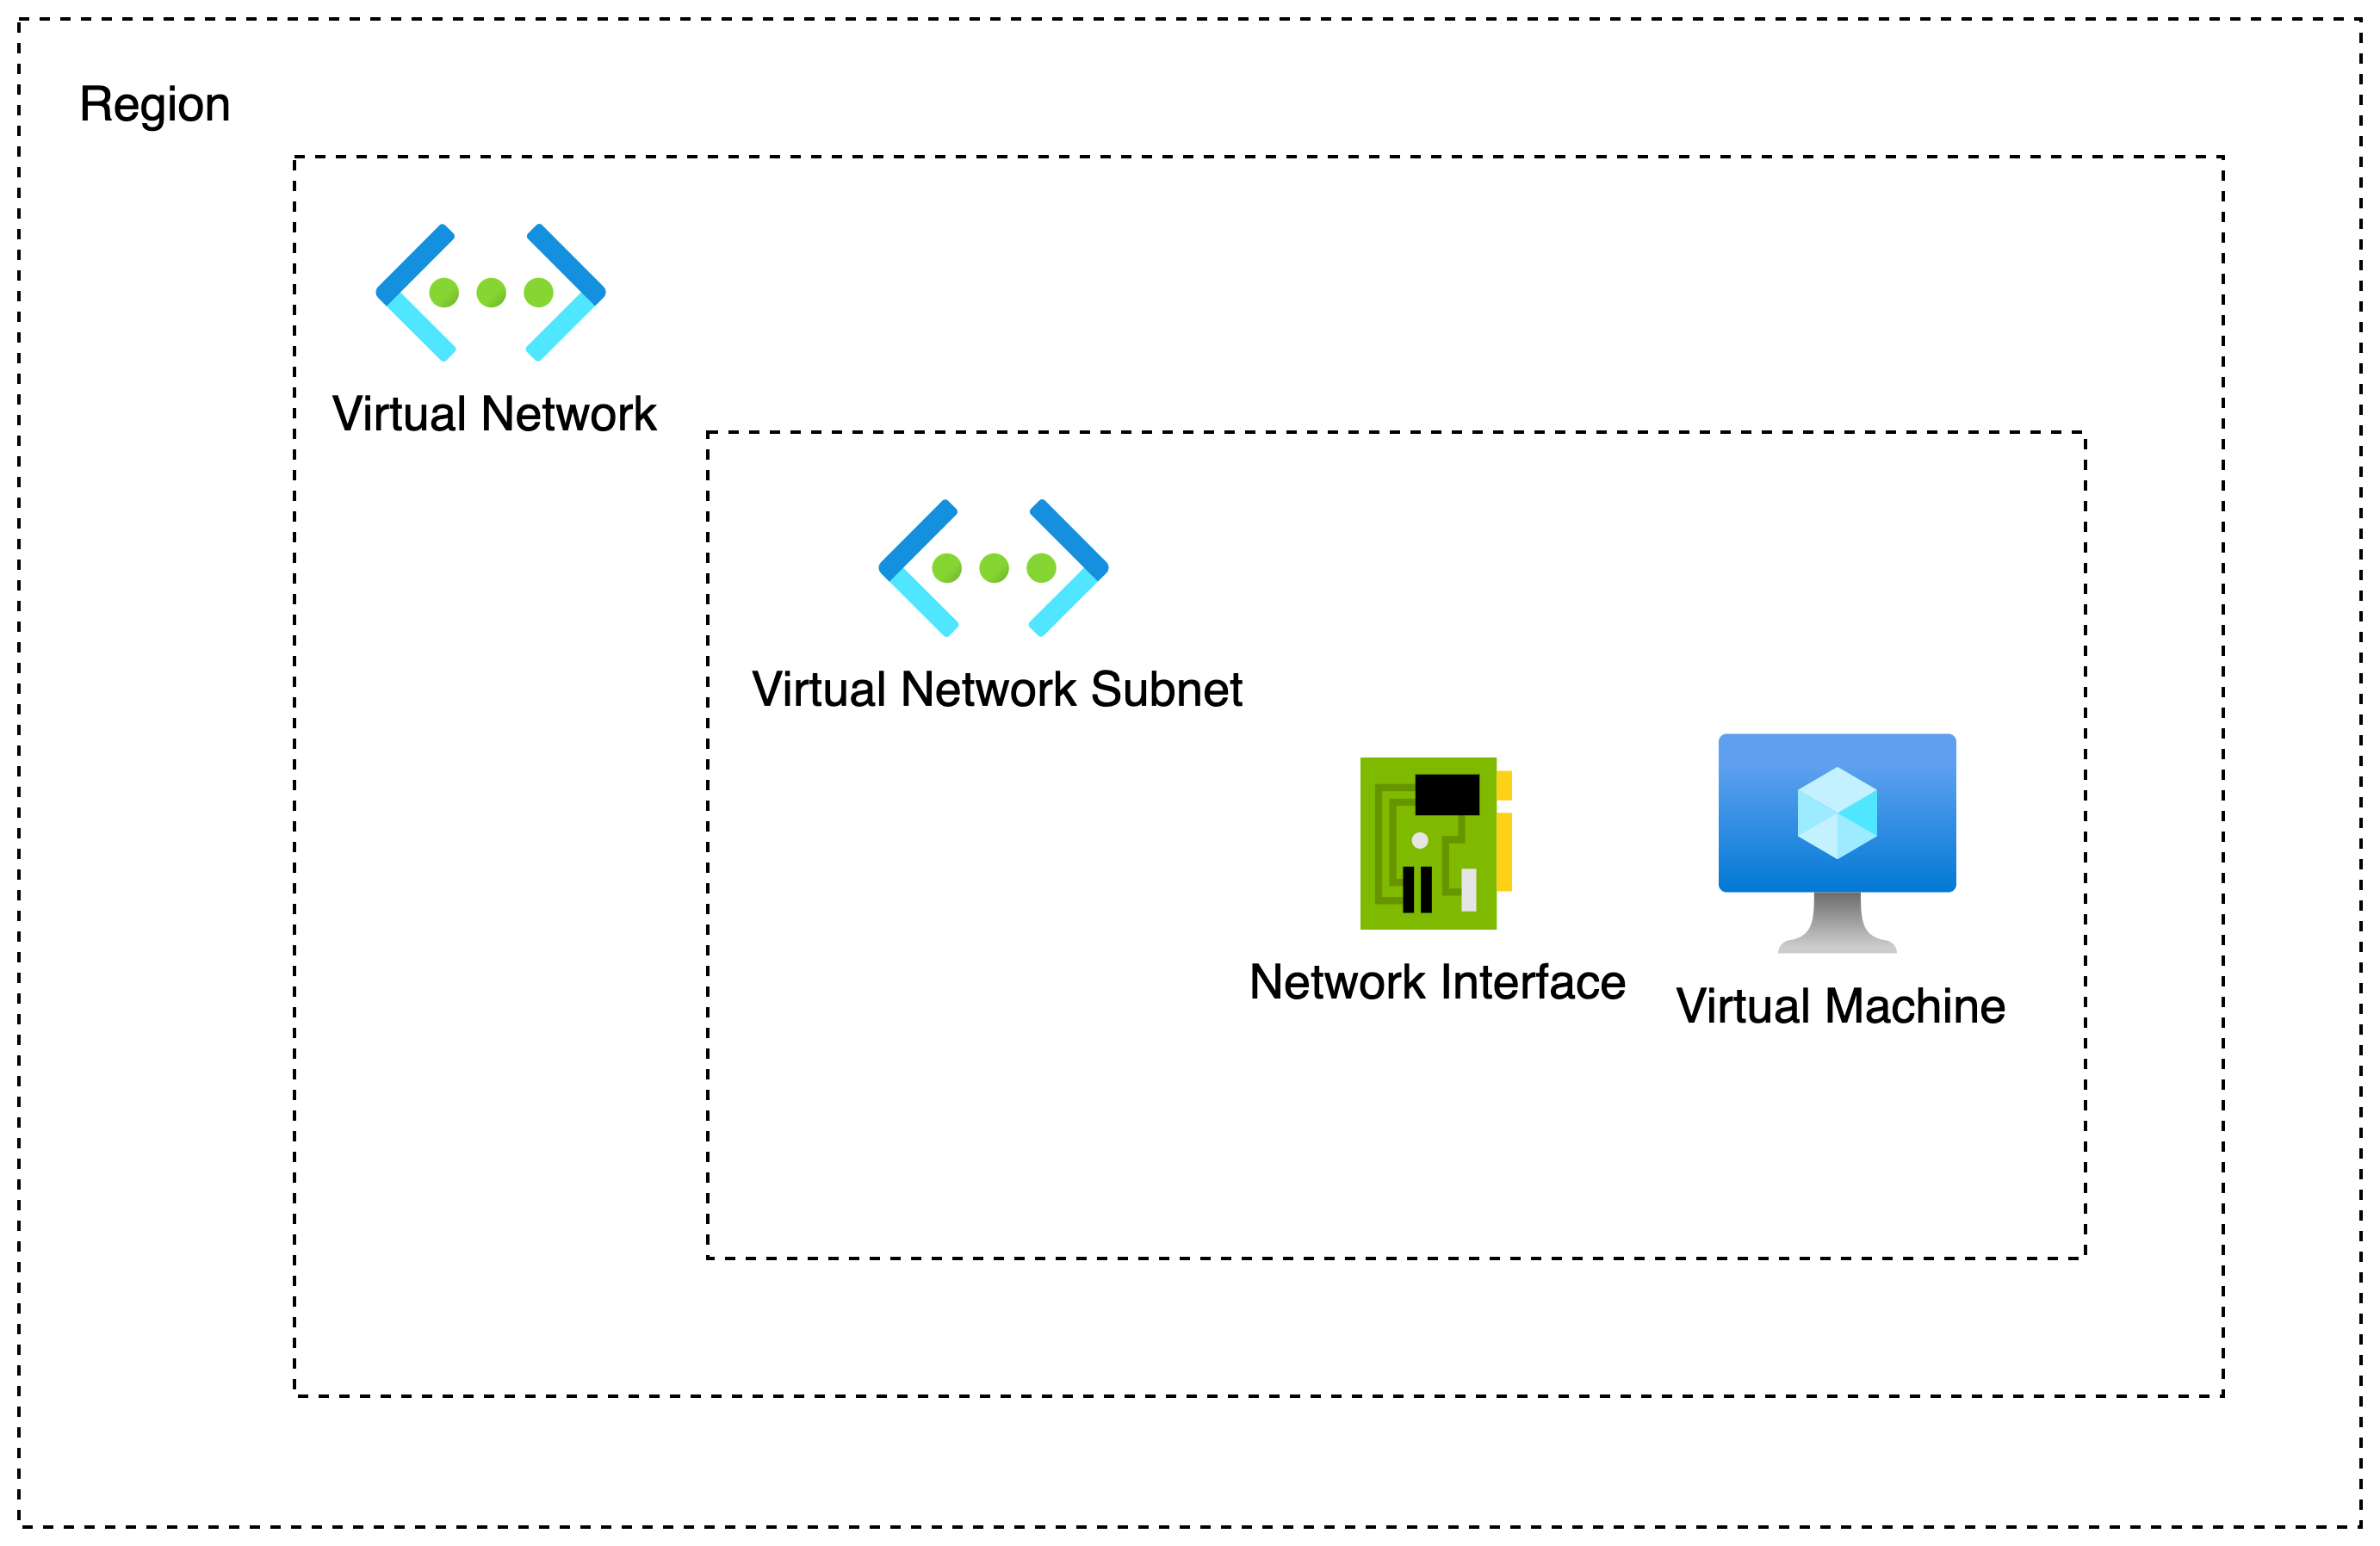
\includegraphics[width=0.75\linewidth]{images/azure.png}
\caption{Minimum set of Azure resources for VM provisioning}
\label{fig:azure}
\end{figure}






INSTANCE CR example











\subsection{GCP Operator}

minimum set of resources needed for vm deployment


\begin{figure}[H]
\centering
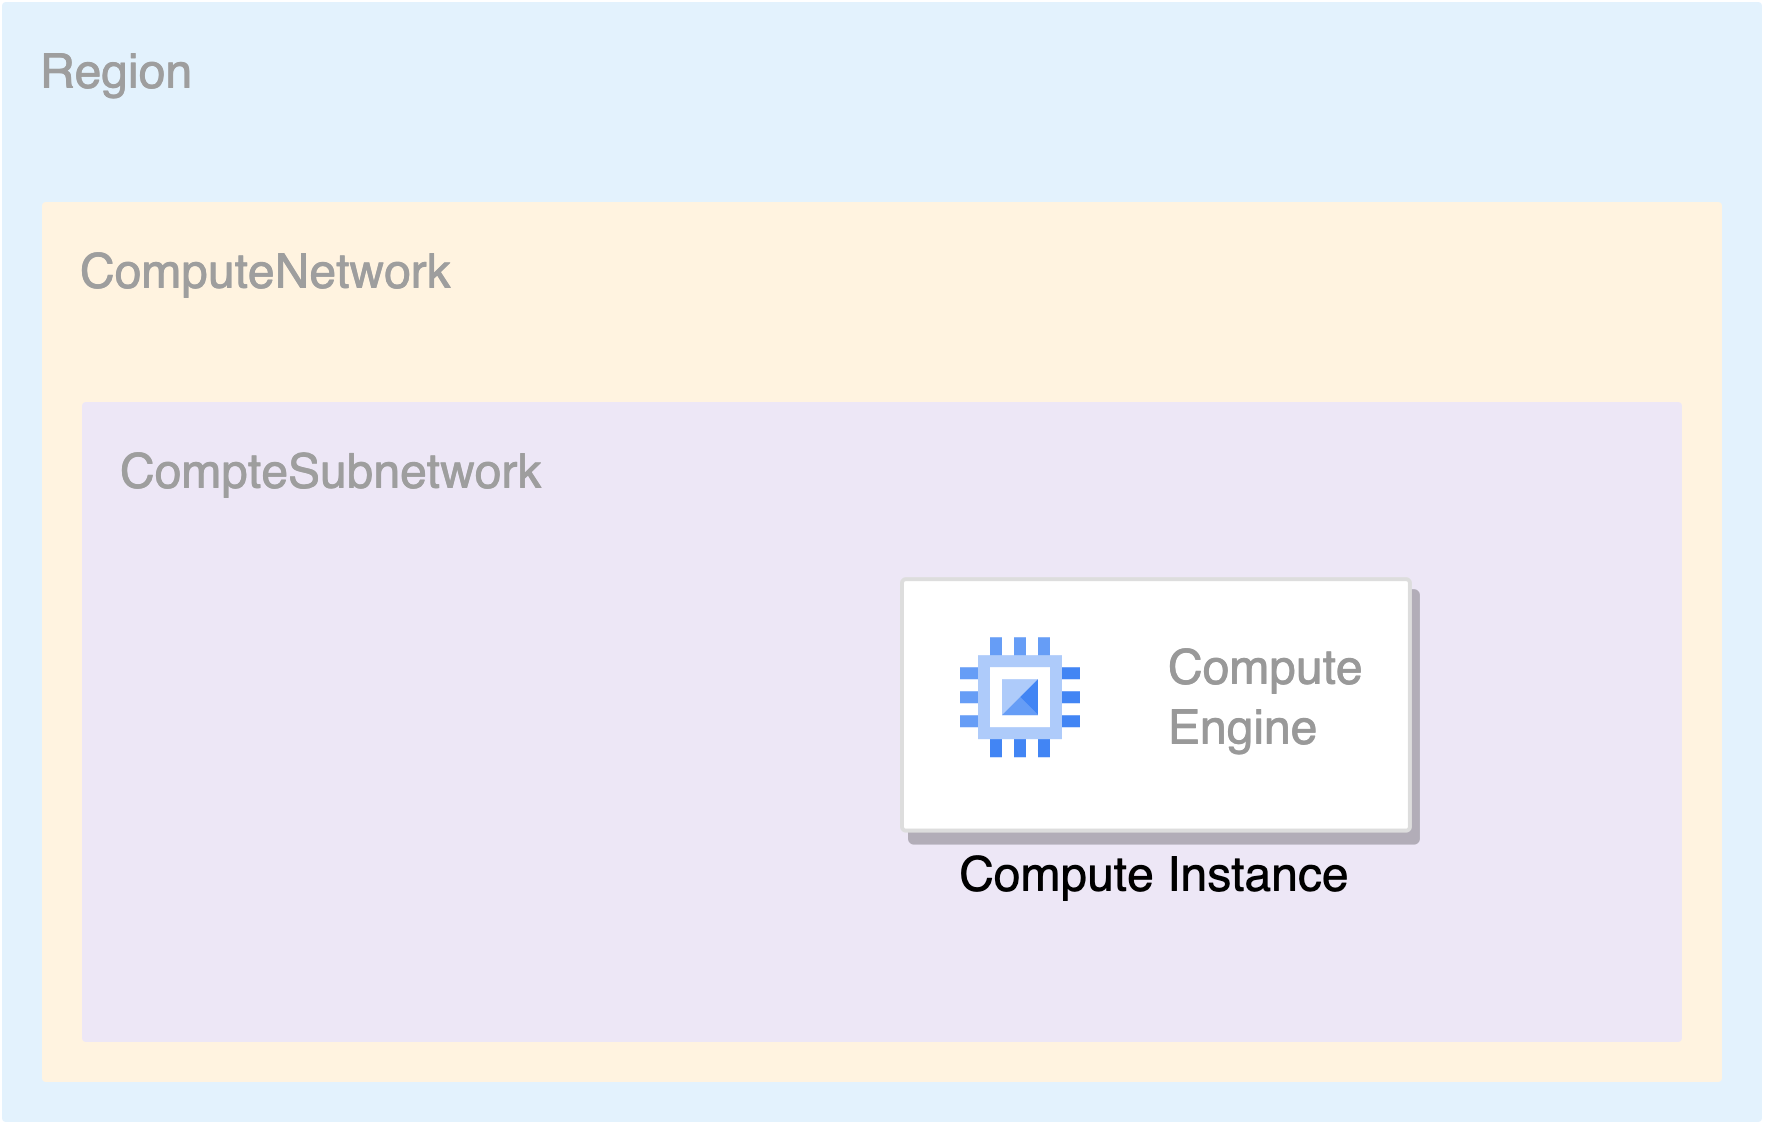
\includegraphics[width=0.75\linewidth]{images/gcp.png}
\caption{Minimum set of GCP resources for VM provisioning}
\label{fig:gcp}
\end{figure}




INSTANCE CR example

some fields are based on regions
some fields are based on zones


networkinterface is directly defined in the instance manifest,
no additional resource needed



\subsection{AWS Operator}

this is a collection of operators that are part of the AWS controllers for Kubernetes (ACK) project.

minimum set of resources needed for vm provisioning

\begin{itemize}[itemsep=0.2pt, topsep=1pt] 
\item[$\bullet$] VPC
\item[$\bullet$] Subnet
\item[$\bullet$] EC2 Instance
\end{itemize}






\begin{figure}[H]
\centering
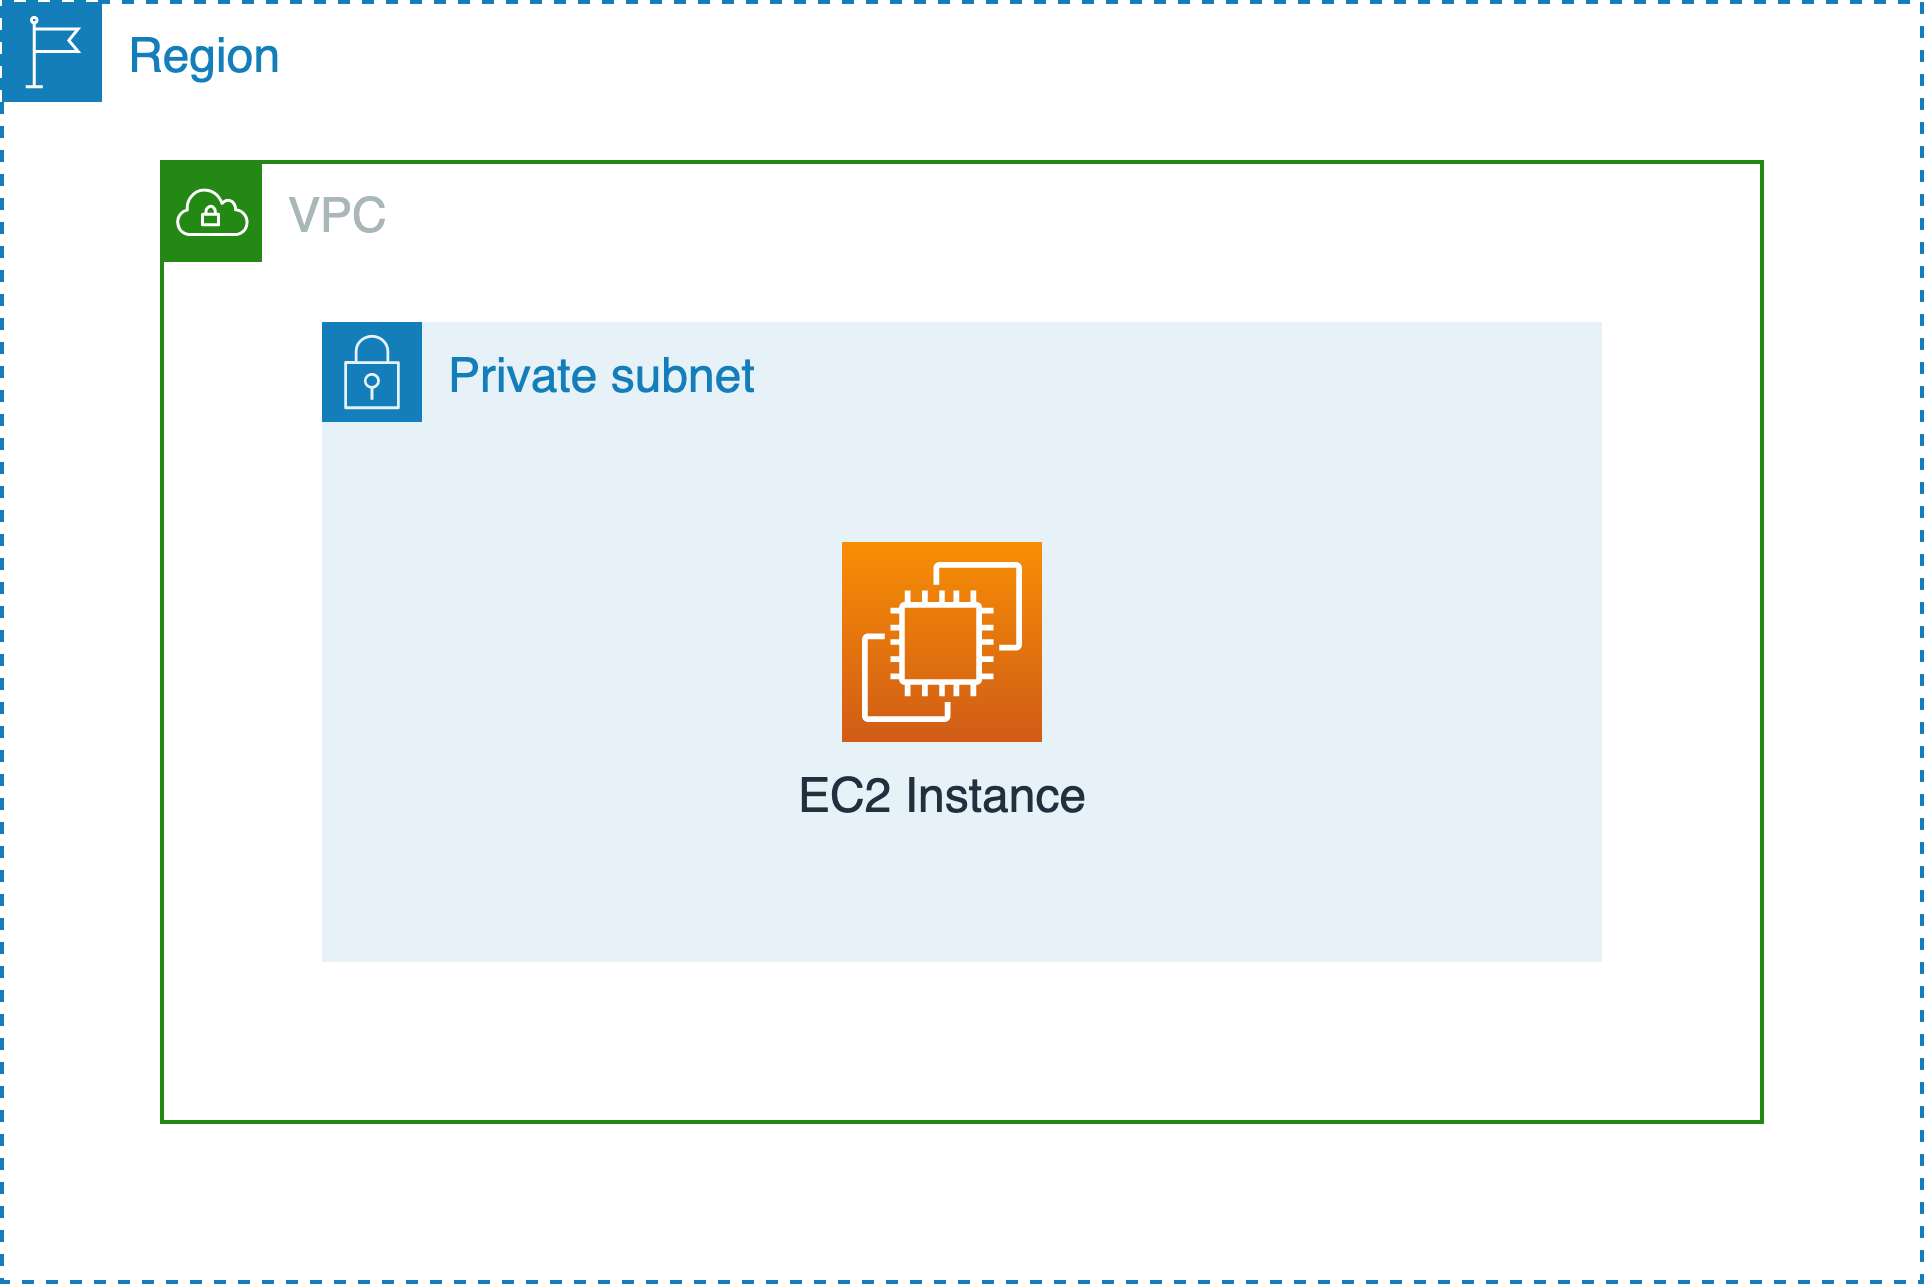
\includegraphics[width=0.75\linewidth]{images/aws.png}
\caption{Minimum set of AWS resources for VM provisioning}
\label{fig:aws}
\end{figure}


As described at the beginning of this section, the implementation approach adopted in our system ensures compatibility with diverse cloud provider design choices. Cloud providers may impose different constraints and best practices when managing Kubernetes-native resources, and the system is designed to adapt to these variations seamlessly.

One notable design choice observed with the AWS operator is the restriction on referencing some Kubernetes objects inside a Custom Resource (CR) manifest. This limitation means that developers cannot directly link a resource (e.g., a Virtual Machine) to another Kubernetes object (e.g., a Subnet) using built-in object references.

To overcome this limitation, our system leverages \textbf{Helm’s \textit{lookup function}}, which dynamically retrieves Kubernetes object details at runtime. This method allows us to fetch required parameters without directly referencing Kubernetes objects in the CR, ensuring compatibility with the AWS operator’s design constraints. The following example demonstrates how the lookup function can be used to resolve subnet IDs dynamically and inject them into the CR manifest. \\

\begin{lstlisting}[language=yaml, caption={Helm Lookup example: dynamically resolving SubnetIDs}, label={lst:helm_lookup}, float=htpb]
...
apiVersion: ec2.services.k8s.aws/v1alpha1
kind: Instance
metadata:
  name: {{ .Values.vmName }}
  namespace: {{ .Values.namespace | default "greenops" }}
...
spec:
  ...
  subnetID: {{ (lookup "ec2.services.k8s.aws/v1alpha1" "Subnet" (.Values.namespace | default "greenops") (printf "%s-subnet" .Values.vmName)).status.subnetID }}
...
\end{lstlisting}

The Helm lookup function can be used to look up resources in a running cluster and its synopsis is: ``lookup apiVersion, kind, namespace, name -> resource or resource list'' \cite{helm_lookup}.
In the listing \ref{lst:helm_lookup}, the Helm lookup function retrieves the subnetID from a Subnet Custom Resource dynamically, based on the VM name and namespace. Then, the subnetID is injected into the Instance Custom Resource manifest, ensuring that the VM is provisioned in the correct subnet.

An example by the same AWS Operator where instead a direct reference to a resource is allowed is the one illustrated in listing \ref{lst:aws_direct_reference}. \\

\begin{lstlisting}[language=yaml, caption={AWS Operator direct reference example}, label={lst:aws_direct_reference}]
...
apiVersion: ec2.services.k8s.aws/v1alpha1
kind: Subnet
metadata:
  name: {{ .Values.vmName }}-subnet
...
spec:
  vpcRef: 
    from: 
      name: {{ .Values.vmName }}-vpc
      namespace: {{ .Values.namespace | default "greenops" }}
...
\end{lstlisting}

In thr case of Listing \ref{lst:aws_direct_reference}, the Subnet Custom Resource manifest directly references in a conveneint way the VPC Custom Resource using its name and namespace since the Operator is designed to support this type of relationship. As explained before, this is determined by Operator design choices but our system is able to handle both scenarios.

\subsubsection{Provider specific configurations}

An Amazon Machine Image (AMI) is a pre-configured image that provides the necessary software environment to set up and boot an Amazon EC2 instance \cite{aws_AMIs}. In other words, AMIs serve as a blueprint for launching virtual machines (VMs) in AWS.

When launching an instance, specifying an AMI is \textbf{mandatory}. The AMI must be compatible with the chosen EC2 instance type, ensuring that the selected image supports the required hardware and software configurations.

The following attributes define an AMI:
\begin{itemize}[itemsep=0.2pt, topsep=1pt] 
  \item[$\bullet$] Region: AMIs are region-specific
  \item[$\bullet$] Operating System: Determines the base OS (e.g., Ubuntu, Windows, RHEL) installed on the AMI.
  \item[$\bullet$] Processor Architecture: e.g., x86, ARM
  \item[$\bullet$] Root Device Type: Specifies whether the AMI uses an EBS-backed volume (Elastic Block Store) or Instance Store for storage.
  \item[$\bullet$] Virtualization Type: Defines whether the AMI supports paravirtual (PV) or hardware virtual machine (HVM) instances.
\end{itemize}


For the purpose of this research, only \textbf{Ubuntu-based AMIs} have been considered for provisioning virtual machines. Official Ubuntu AMIs were collected from a dedicated Ubuntu repository.
In order to select the most suitable AMI for a given VM, the system leverages Helm template engine to dynamically select the appropriate AMI ID based on the region and other parameters specified in the VmTemplate Kubernetes Custom Resource (CR).



\newpage

\section{Open Policy Agent (OPA)}

Open Policy Agent (OPA) is an open-source general-purpose \textbf{policy engine} that enables unified policy enforcement across cloud-native environments. OPA provides a declarative language called Rego enabling a paradigm known as ``\textbf{Policy as Code}" \cite{opa_docs}.

Open Policy Agent can be integrated as a sidecar container, host-level daemon, or library to perform policy decisions for a plethora of use cases: microservices, Kubernetes admission control, CI/CD pipelines, API gateways and more \cite{opa_docs}. 

In the context of our system, OPA and the Policy-as-Code paradigm are used to enforce policies for workload scheduling: encoding the output of a scheduling decision coming from an external GreenOps Scheduler and ensuring compliance with additional policies related to latency requirements and legal constraints.

\subsection{Policy as Code paradigm}

According to AWS, Policy-as-Code (PaC) is a software automation approach which is similar to Infrastructure-as-Code (IaC) \cite{pac_aws}. PaC helps assess company system configurations and validate compliance requirements through software automation \cite{pac_aws}. The perceived value of this type of automation in the software development lifecycle has grown significantly in modern enterprises. This large adoption is probably driven by the inherent consistency and reliability it provides, ensuring standardized enforcement of policies and reducing human error \cite{pac_aws}.

OPA's generic defintion of policy is: ``\textit{A policy is a set of rules that governs the behavior of a software service}" \cite{opa_philosophy}. OPA provides a high-level declarative language called \textbf{Rego} to define policies in a flexible manner. One of OPA's key strengths is its \textbf{domain-agnostic design}, allowing it to enforce policies across various systems and environments. This makes it highly adaptable to different use cases, ranging from access control to infrastructure security. Some representative examples of policies that OPA can enforce include:

\begin{itemize}[itemsep=0.2pt, topsep=1pt] \item[$\bullet$] Restricting which image registries can be used for deploying new Pods in a Kubernetes cluster.
\item[$\bullet$] Controlling whether a specific user is permitted to perform delete operations on certain resources.
\item[$\bullet$] Enforcing network security policies, such as blocking external access to sensitive services.
\item[$\bullet$] Ensuring infrastructure compliance, for example, by verifying that new cloud resources to be provisioned follow predefined security configurations.
\item[$\bullet$] Enforcing that new deployed servers must have the prefix ``server-" in their name.
\end{itemize}

Therefore, the use cases covered span from role-based access control to container image security and beyond.
\newline


Another important aspect of OPA is that it effectively \textbf{decouples} policy decision-making from policy enforcement, enabling organizations to implement consistent and scalable authorization across their systems \cite{test}.
In practice, this means that when a software module needs to make a policy decision, it queries OPA, supplying relevant data as input. In other words, policy decisions are \textbf{offloaded} to OPA rather than being hardcoded within individual services. This approach offers several key advantages:
\begin{itemize}[itemsep=0.2pt, topsep=1pt]
  \item[$\bullet$] \textbf{Centralized policy management}: policies are defined in a single location, ensuring uniform enforcement across all services.
  \item[$\bullet$] \textbf{Improved maintainability}: updating policies does not require modifying, recompiling or redeploying application code, reducing complexity and deployment overhead.
  \item[$\bullet$] \textbf{Greater flexibility}: policies can be dynamically updated (e.g., with CI/CD approaches) based on evolving security and compliance requirements 
  \item[$\bullet$] \textbf{Scalability}: since OPA and application modules are not tightly coupled.
\end{itemize} 

\subsection{OPA architecture overview}

As mentioned in the introduction to this section, one common approach to integrating OPA into a software system is by deploying it as a host-level daemon. The latter is essentially a lightweight server that processes policy queries via HTTP requests. This setup allows services to offload policy decision-making to OPA in a scalable and efficient manner since the two entities are not tightly coupled.

A standard OPA deployment consists of three main components:

\begin{itemize}[itemsep=0.2pt, topsep=1pt]
\item[$\bullet$] \textbf{OPA Server} – The core service that evaluates policy queries and returns decisions based on defined rules, contextual data and input data.
\item[$\bullet$] \textbf{OPA Policies} – Rules written in the Rego language that define the logic to be enforced.
\item[$\bullet$] \textbf{Data} – Optional contextual information, typically structured in JSON format, that policies use to make informed decisions along with input data.
\end{itemize}

To facilitate deployment and management, Rego policies and associated contextual data are packaged into \textbf{policy bundles}, as described in section \ref{sec:opa_policies}. These bundles enable version-controlled, centralized policy distribution, ensuring consistency and maintainability across distributed environments. \newline


\begin{figure}[htb]
\centering
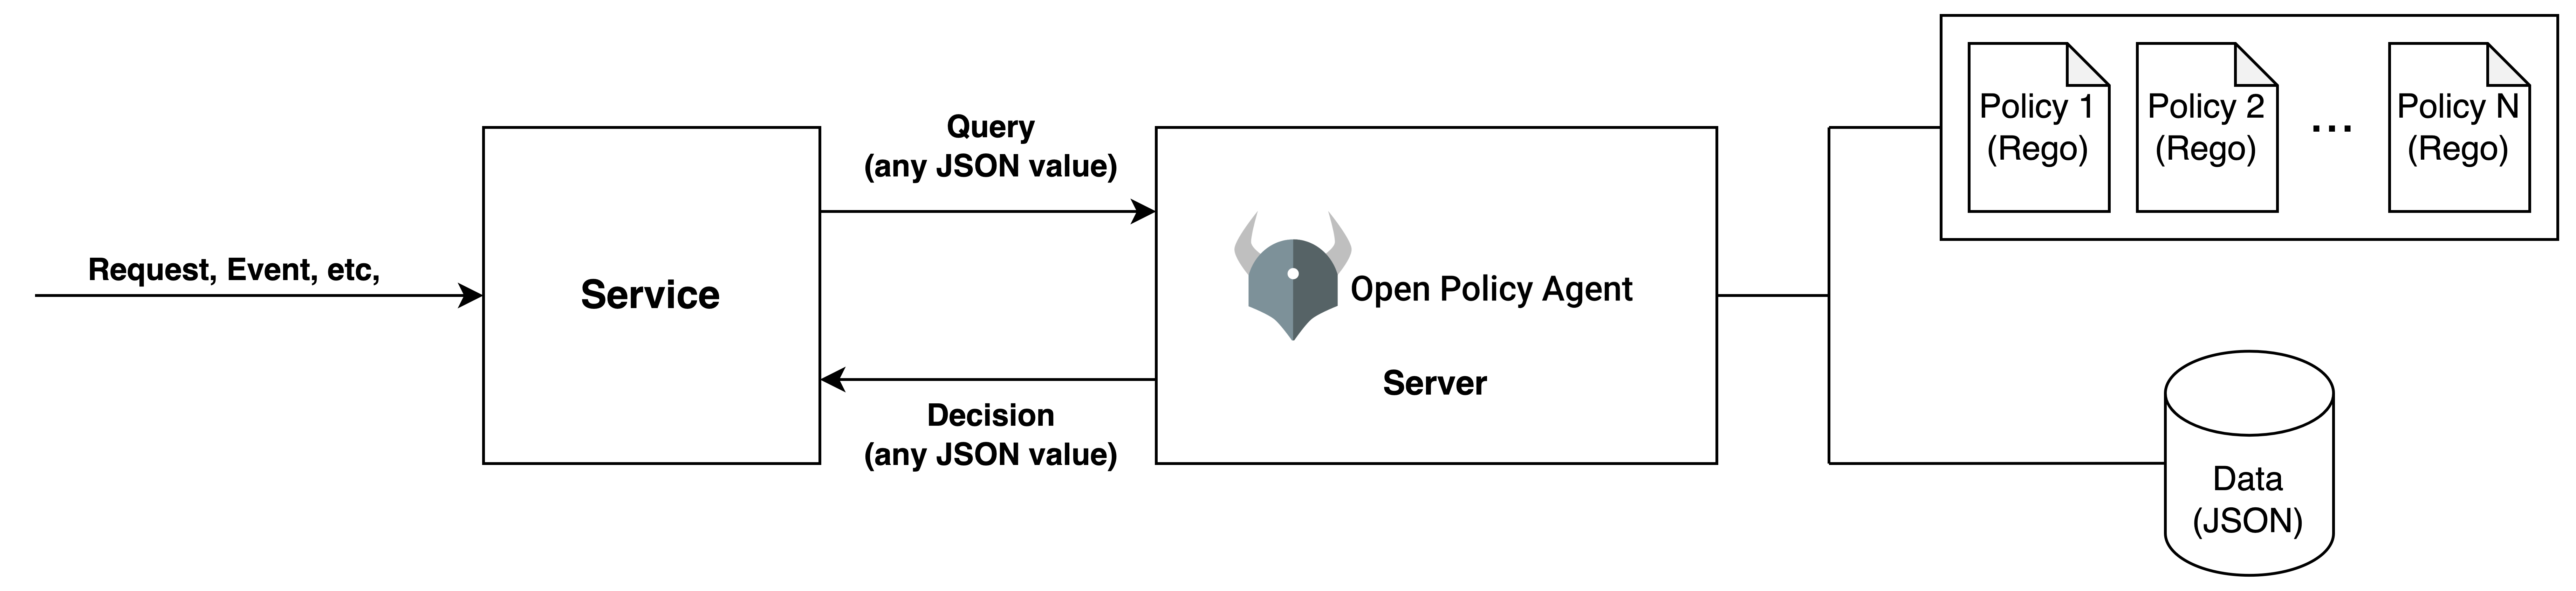
\includegraphics[width=1\linewidth]{images/OPA.png}
\caption{OPA architecture}
\label{fig:opa_architecture}
\end{figure}


OPA accepts arbitrary structured data as input.
and  Like query inputs, your policies can generate arbitrary structured data as output.

\subsection{OPA and external data}

types of external data strategies

http.send()
paramters 

\subsection{OPA integration with Kubernetes}

In Kubernetes admission control, policy enforcement is handled by the \textbf{Kubernetes API server} itself. OPA makes the policy decisions when queried by the admission controller, but the actual enforcement (namely allowing or denying requests) is executed by Kubernetes' built-in admission control mechanisms. This workflow is represented in figure \ref{fig:webhook_opa} where \textbf{AdmissionrReview request} and \textbf{AdmissionReview response} are respectively input and output of the whole OPA section. The API Server sends the entire Kubernetes object in the webhook request to OPA. %cite OPA kubernetes primer
The Kubernetes API server will use the received AdmissionReview response for its decision. \\
%\cite{opa_philosophy}

\begin{figure}[htb]
\centering
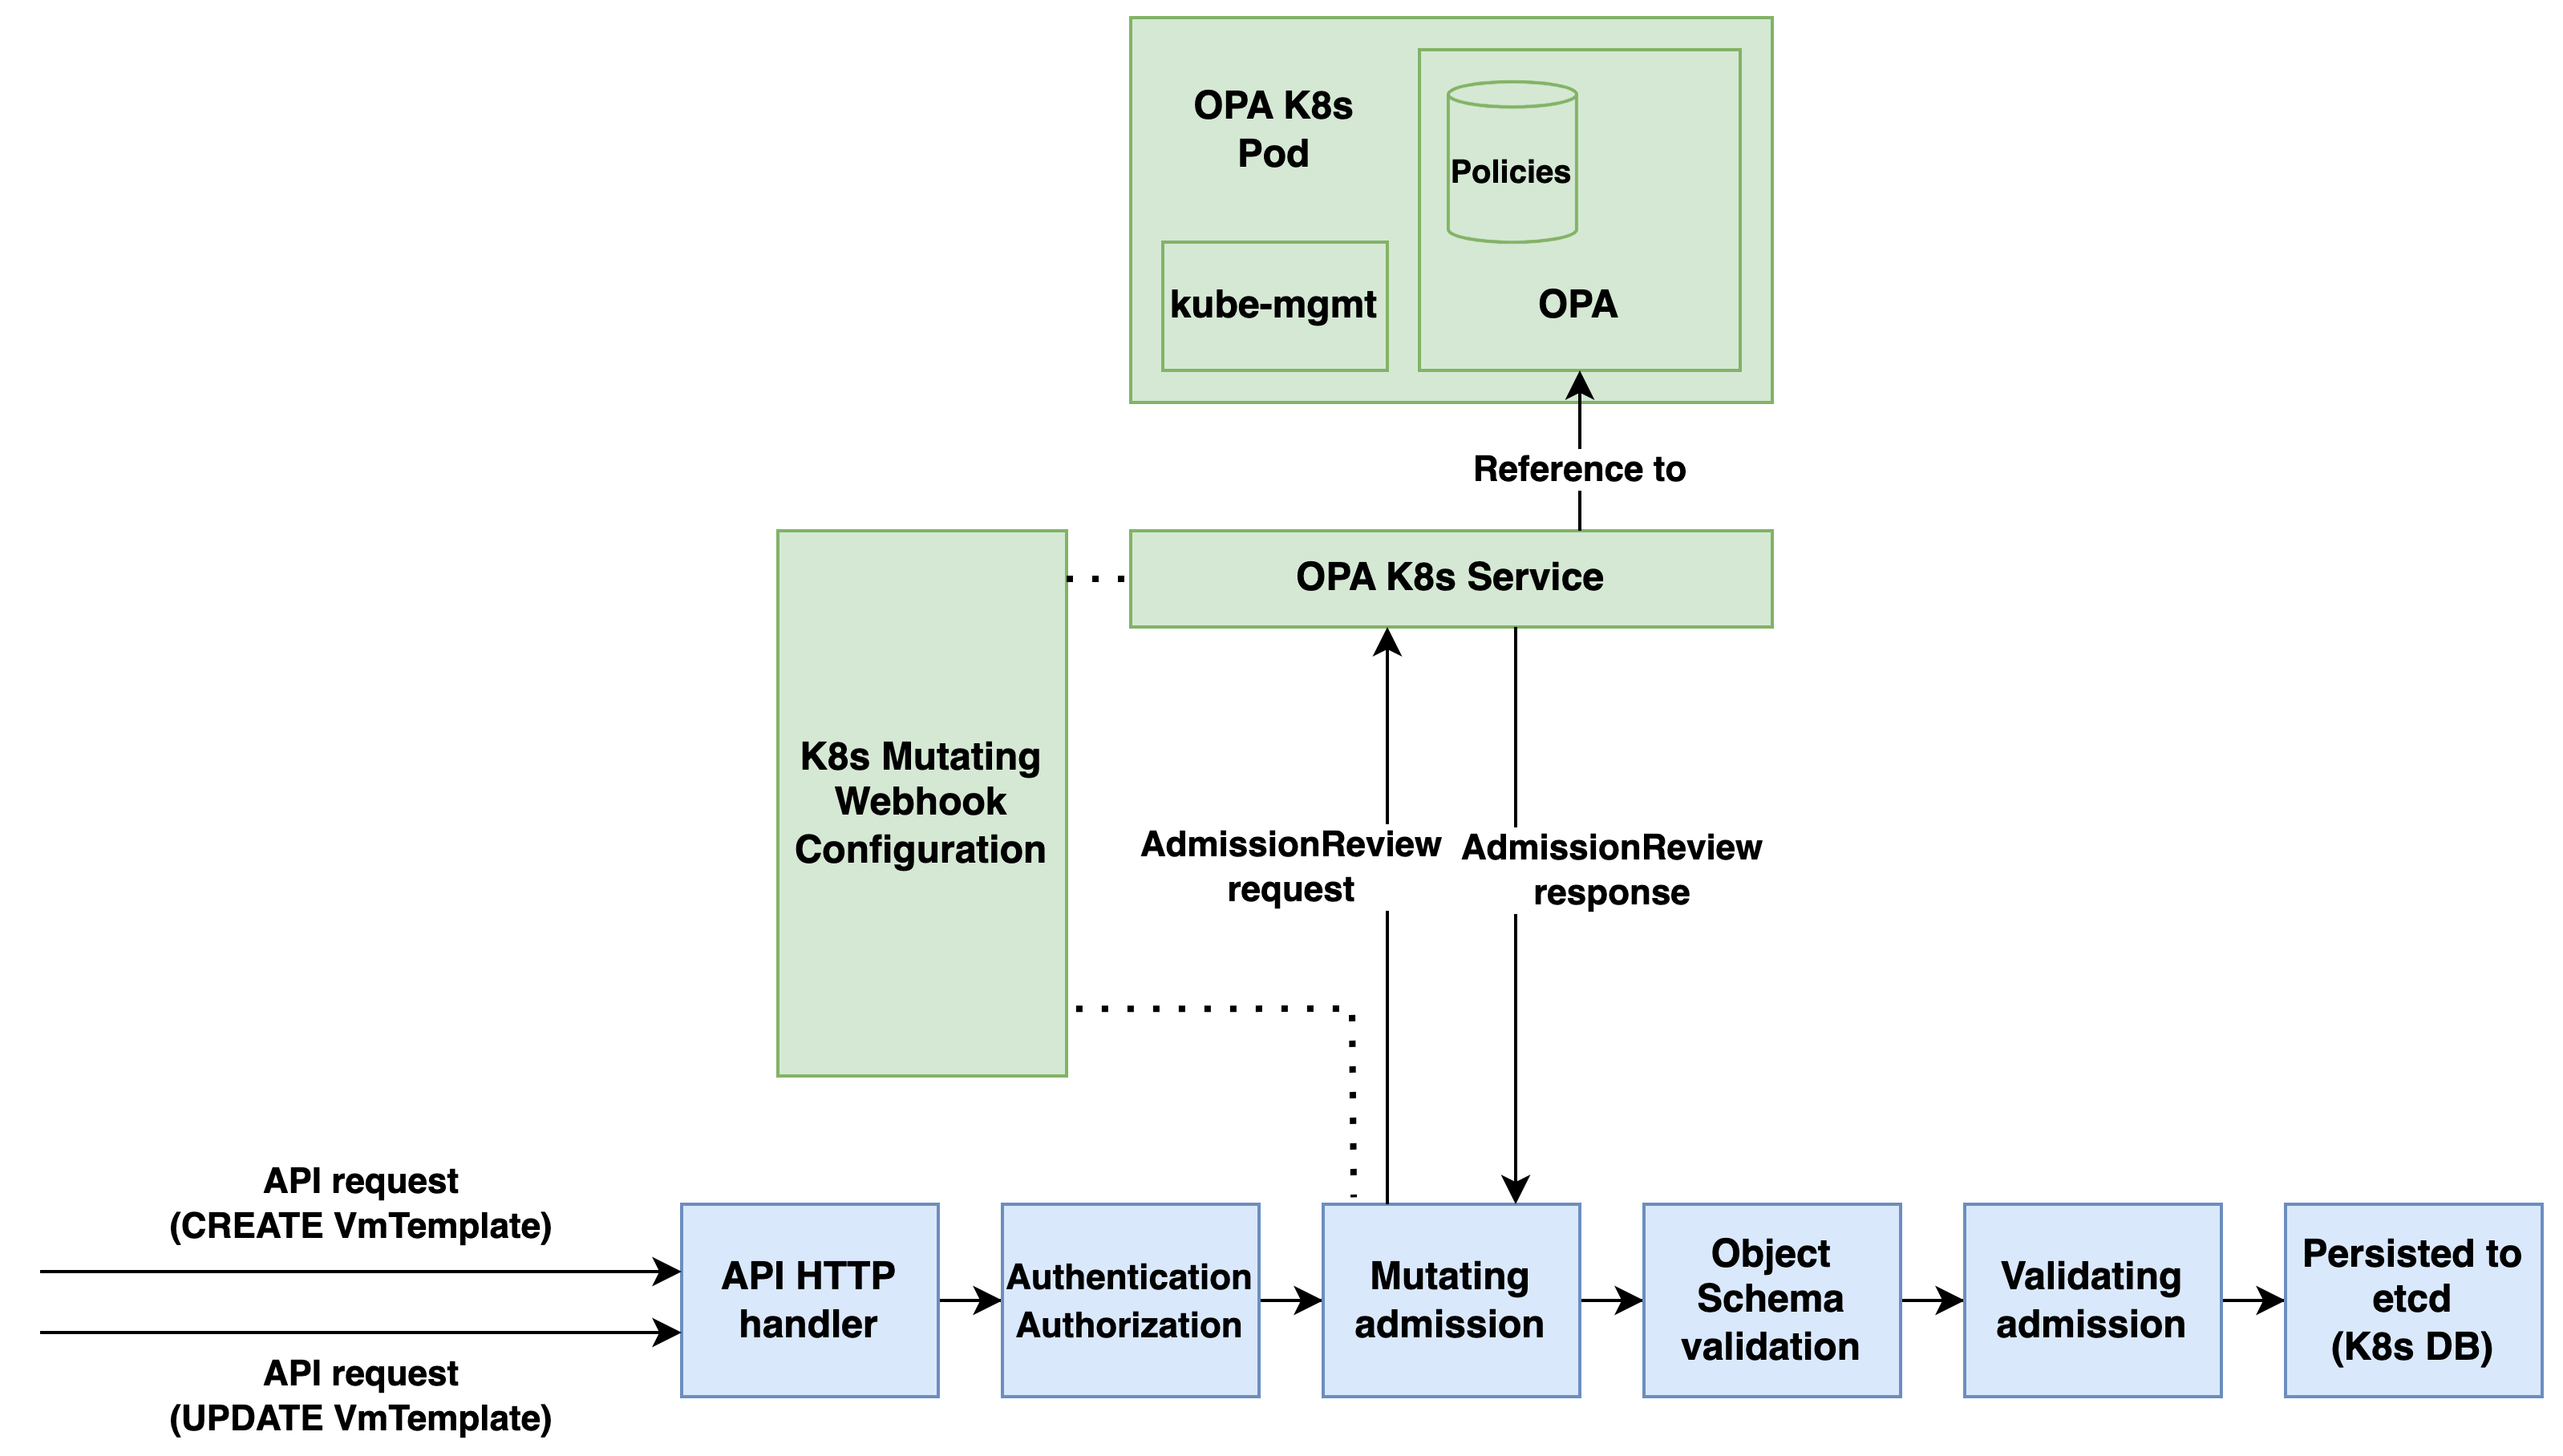
\includegraphics[width=1\linewidth]{images/webhook.png}
\caption{Kubernetes mutating webhook and OPA integration}
\label{fig:webhook_opa}
\end{figure}

In a Kubernetes deployment, an OPA Pod typically consists of the following containers:
\begin{itemize}[itemsep=0.2pt, topsep=1pt]
  \item[$\bullet$] OPA server container
  \item[$\bullet$] \textbf{kube-mgmt} container \\
\end{itemize} 

The kube-mgmt container functions as a \textbf{sidecar container} within a Kubernetes Pod. The sidecar container pattern is a common Kubernetes design paradigm in which auxiliary containers run alongside the main application container within the same Pod. These additional containers serve to enhance, extend, or support the primary application's functionality without modifying its core logic \cite{sidecar_containers}. 
The primary responsibility of kube-mgmt is to replicate Kubernetes resources into the OPA instance (OPA container). This operation is essential for OPA to access and evaluate policies based on real-time cluster state, enabling dynamic policy enforcement. By synchronizing these resources, kube-mgmt ensures that OPA has an up-to-date view of relevant Kubernetes objects.
This is especially useful to enforce policies that deals with naming conflicts, where OPA needs to check existing names in the cluster for the decision \cite{kube-mgmt}.
Additionally, it allows for loading policies directly from the Kubernetes cluster by retrieving them in the form of ConfigMaps. This feature is particularly useful when policies need to be dynamically updated based on the current state of the cluster \cite{kube-mgmt}. However, in the system described in this thesis, this latter feature is not employed in the current implementation as we are using policy bundles for policy distribution.

In the current system configuration, the kube-mgmt container is deployed to facilitate resource replication, ensuring that Kubernetes resources, namely VmTemplate resources, are synchronized with the OPA instance. However, at present, no policy requires interrogation of VmTemplate resources that are already present in the system.
Looking ahead, future policies could leverage VmTemplate resource information to enforce naming conflict resolution, quota management, or additional constraints.

\newpage

\subsection{OPA policies}
\label{sec:opa_policies}

%example of a policy:
%(https://www.openpolicyagent.org/docs/latest/kubernetes-primer/)





As OPA official documentation describes, when the Kubernetes AdmissionReview request from the webhook arrives, it is binded to the OPA input document and generates the default, ``root", decision: \textit{system.main}
%\cite

The root policy, in the case of Kubernetes admission control, is responsible for generating the AdmissionReview response in accordance with the Kubernetes API specifications. It is the duty of the policy developer to write Rego code that produces a well-formed AdmissionReview response, ensuring that the OPA server can then correctly communicate its decision to the Kubernetes admission controller.
%cite

It is deemed useful to show one of the simplest and common example of a OPA policy in the \textbf{Kubernetes admission control context}. That is: to ensure all images for Kubernetes Pods come from a trusted registry, namely \textit{unitn.it}. \\


It is important to note that, in this case, due to the simplicity of the policy, no additional contextual data in JSON format is required.


policy compilation
policy are compiled
compile time errors like merge errors if data is clashing for instance



\begin{comment}
    \lstset{
   language=Go,
   basicstyle=\ttfamily\small,
   breaklines=true,
   showstringspaces=false,
   commentstyle=\color{green!60!black},
   keywordstyle=\color{blue},
   stringstyle=\color{purple},
   numberstyle=\tiny,
   numbers=left,
   backgroundcolor=\color{gray!10},
   frame=single,
   captionpos=b
}
\end{comment}


\begin{lstlisting}[language=Rego, caption={Rego policy for Pods registry},
label=lst:rego_data_mapping]                              
deny contains msg if {                                                      
    input.request.kind.kind == "Pod"                                        
    image := input.request.object.spec.containers[_].image                  
    not startswith(image, "unitn.it/")                                     
    msg := sprintf("image '%v' comes from untrusted registry", [image])     
}
\end{lstlisting}

\begin{lstlisting}[language=Rego, caption={Rego ``root" policy (system.main)}]
package system

import data.kubernetes.admission

main := {
	"apiVersion": "admission.k8s.io/v1",
	"kind": "AdmissionReview",
	"response": response,
}

default uid := ""

uid := input.request.uid

response := {
	"allowed": false,
	"uid": uid,
	"status": {"message": reason},
} if {
	reason := concat(", ", admission.deny)
	reason != ""
}

else := {"allowed": true, "uid": uid}
\end{lstlisting}


\newpage
\lstset{style=jsonstyle}
\begin{lstlisting}[caption={AdmissionReview request}]
{
    "apiVersion": "admission.k8s.io/v1",
    "kind": "AdmissionReview",
    "request": {
        "kind": {
            "group": "",
            "kind": "Pod",
            "version": "v1"
        },
        "object": {
            "metadata": {
                "name": "myapp"
            },
            "spec": {
                "containers": [
                    {
                        "image": "bitnami/node:22",
                        "name": "nodejs"
                    }
                ]
            }
        }
    }
}
\end{lstlisting}

\lstset{style=jsonstyle}
\begin{lstlisting}[caption={AdmissionReview response}]
{
    "apiVersion": "admission.k8s.io/v1",
    "kind": "AdmissionReview",
    "response": {
        "allowed": false
        "status": {
            "message": "image 'bitnami/node:22' comes from untrusted registry"
        }
    }
}
\end{lstlisting}

Therefore, in this specific case, the creation of the Kubernetes Pod will be \textbf{denied}. OPA is responsible for \textbf{decision-making}, determining that the request do not complies with the defined policies, while the Kubernetes API server, using the AdmissionReview response generated by OPA, handles \textbf{policy enforcement}, effectively rejecting the CREATE request since it violates the specified rules.

\subsection{OPA Policy bundles}
\label{sec:opa_bundles}

An OPA policy bundle is a collection of policies and optional associated contextual data. More precisely, a bundle is a standardized way to package policies, facilitating version control and distribution \cite{opa_bundles}. As a matter of fact, a single policy bundle can be potentially used by multiple OPA instances.
A policy bundle mainly consists of:
\begin{itemize}[itemsep=0.2pt, topsep=1pt]
  \item[$\bullet$] \textbf{Rego policy files} defining the logic.
  \item[$\bullet$] \textbf{Data files} (in JSON or YAML format) containing contextual information required for policy evaluation (e.g., cloud region mappings).
\end{itemize} 

Policy bundles can be distributed through a variety of mechanisms such as remote HTTP servers (e.g., NGINX) and object storage services (e.g., Amazon S3, Google Cloud Storage, Azure Blob Storage) \cite{opa_bundles}.
One of the most convenient approaches is packaging them as \textbf{OCI (Open Container Initiative) images} \cite{oci} and this is the approach adopted in the system described in this thesis.

Once packaged as OCI images, policy bundles can be pulled by OPA servers from a container registry at predefined time intervals. This allows policy updates to be deployed in OPA \textbf{without requiring manual intervention} or \textbf{service restarts}, ensuring that enforcement mechanisms remain up to date with the latest compliance requirements identified and implemented by the organization. This is crucial for instance when dealing with \textbf{critical security policies} that need to be updated frequently, maybe in response to the discoveries of new CVEs. In the context of our system, such timely updates are not essential but the OPA is designed to be able to handle them if needed.
To ensure continuous policy enforcement while maintaining high operational efficiency, a CI/CD approach is adopted for policy management in the context of our system.
As a matter of fact, policies are maintained in a \textbf{version-controlled hosted repository} (i.e., on GitHub), where updates like tagging (``git tag'') trigger an automated pipeline (e.g., using GitHub Actions) responsible for building, packaging into a OCI image, and publishing the policy bundle to a container registry (e.g., Docker Hub).
One of the major advantages of this approach is the ability to dynamically update policies without requiring OPA pods to restart as there is an \textbf{hot-reload} of policies done at application level by OPA (``loaded on the fly'') \cite{opa_bundles}. This is particularly useful in production environments where service availability is critical and downtime must be minimized. 
The overall process of policy distribution is illustrated in figure \ref{fig:opa_bundles}.

\begin{figure}[H]
\centering
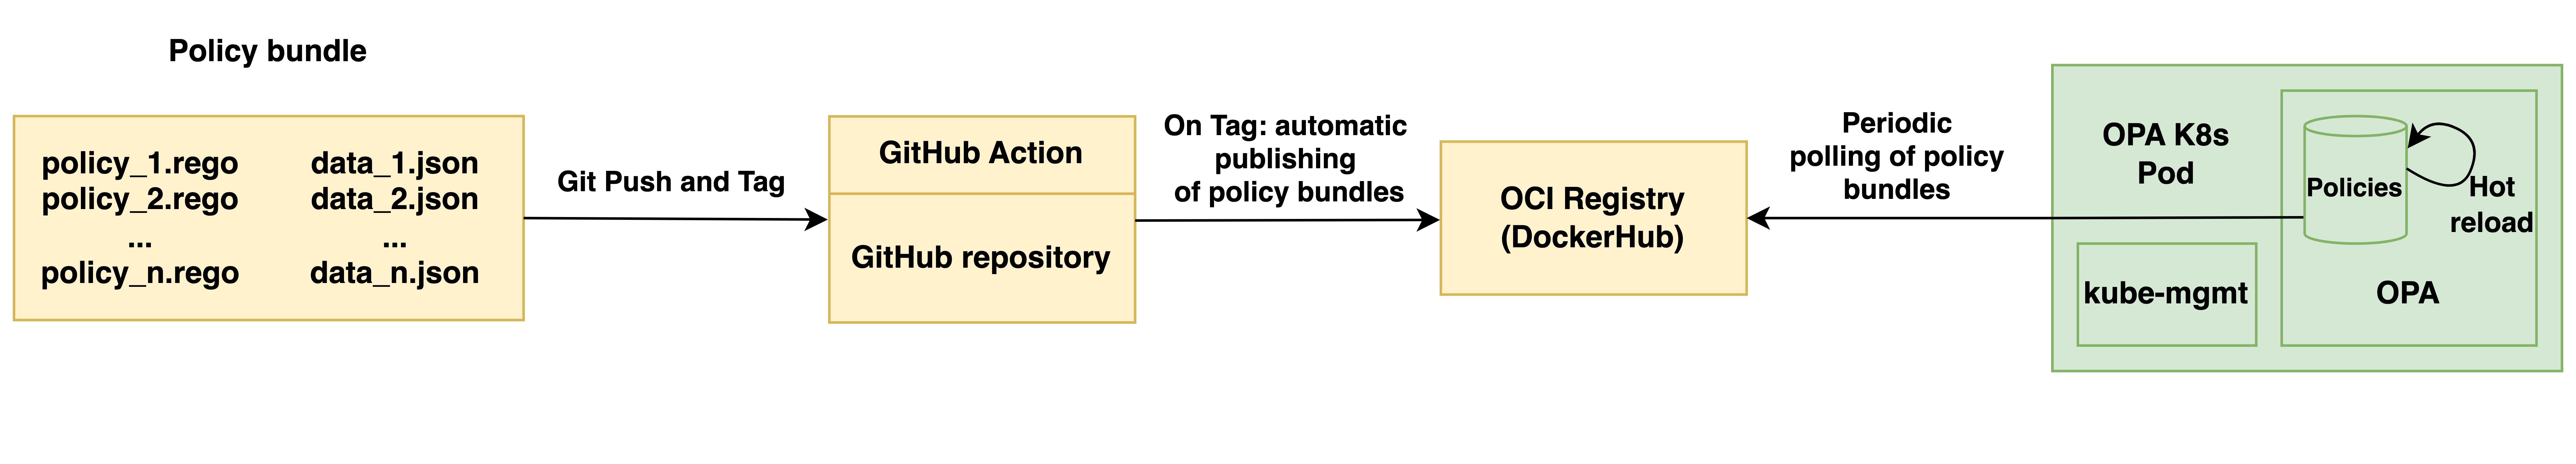
\includegraphics[width=1\linewidth]{images/opa_bundles.png}
\caption{OPA policy bundles}
\label{fig:opa_bundles}
\end{figure}

By leveraging OCI images for policy distribution and implementing a fully automated CI/CD pipeline, our system ensures that policy enforcement remains consistent, up to date, and highly available across all OPA instances. This approach aligns with modern DevOps practices, enabling organizations to maintain a high level of security and compliance without compromising operational efficiency.

\newpage

\subsection{OPA Gatekeeper}

OPA Gatekeeper is a Kubernetes-native policy engine that extends OPA with \textbf{Custom Resources (CRs)} and controllers to enforce policies across a Kubernetes cluster. It integrates natively with Kubernetes and provides a declarative approach to defining and enforcing policies using Kubernetes Custom Resources (CRs). This makes it an excellent choice for basic and standard policy enforcement scenarios, such as RBAC (Role-Based Access Control), security compliance, and resource constraints.
However, while OPA Gatekeeper is well-suited for simple use cases, it presents \textbf{limitations} when addressing complex policy requirements, particularly when policies involve \textbf{mutations} or require access to \textbf{external data sources}. These limitations make it unsuitable for the specific challenges tackled in this system. Therefore, after an initial investigation and Proof of Concept implementation, we decided to use the standard OPA server for policy enforcement mainly due to the flexibility it provides in handling diverse scenarios.

To illustrate the differences between a standard OPA policy and an OPA Gatekeeper policy, we present two examples:  
\begin{itemize}[itemsep=0.2pt, topsep=1pt]
  \item[$\bullet$] a simple Rego policy that enforces a basic constraint on Pod creation in a Kubernetes cluster.
  \item[$\bullet$] the corresponding policy implemented as an OPA Gatekeeper \textbf{ConstraintTemplate} and \textbf{Constraint} Kubernetes resources.
\end{itemize}

The first example demonstrates a standalone Rego policy, which can be evaluated directly by an OPA instance. While this approach is flexible and allows for fine-grained policy definition, it requires manual integration into the system, including policy distribution and enforcement setup.  

\lstset{style=python}
\begin{lstlisting}[language=rego, caption={Simple OPA Rego Policy}, label={lst:opa-rego}]
package kubernetes.admission

deny[msg] {
  input.request.kind.kind == "Pod"
  input.request.object.metadata.namespace == "restricted"
  msg := "Pods cannot be created in the 'restricted' namespace."
}
\end{lstlisting}

The second example, illustrated in listing \ref{lst:gatekeeper-template} utilizes OPA Gatekeeper, which extends Kubernetes with Kubernetes-native Custom Resource Definitions (CRDs), enabling declarative policy management. By using a ConstraintTemplate, policies can be enforced dynamically through Kubernetes, making them easier to distribute and manage.
In other words, with this kind of setting, OPA policy bundles are not employed in the same way as in the standard OPA server. Instead, policies are defined as Kubernetes resources, allowing for more straightforward policy enforcement and management within a Kubernetes environment.

\begin{lstlisting}[language=yaml, caption={OPA Gatekeeper ConstraintTemplate}, label={lst:gatekeeper-template}]
apiVersion: templates.gatekeeper.sh/v1
kind: ConstraintTemplate
metadata:
  name: podnamespaceconstraint
spec:
  crd:
    spec:
      names:
        kind: PodNamespaceConstraint
  targets:
    - target: admission.k8s.gatekeeper.sh
      rego: |
        package kubernetes.admission
        deny[msg] {
          input.review.object.metadata.namespace == "restricted"
          msg := "Pods cannot be created in the 'restricted' namespace."
        }
\end{lstlisting}

\begin{lstlisting}[language=yaml, caption={OPA Gatekeeper Constraint}, label={lst:gatekeeper-constraint}, float=htpb]
apiVersion: constraints.gatekeeper.sh/v1beta1
kind: PodNamespaceConstraint
metadata:
  name: restrict-namespace
spec:
  match:
    kinds:
      - apiGroups: [""]
        kinds: ["Pod"]
  parameters: {}
\end{lstlisting}

In the example, the policy is defined as a ConstraintTemplate, which is then instantiated as a Constraint Custom Resource of kind defined in the ConstraintTemplate. The ConstraintTemplate specifies the Rego policy logic, while the Constraint defines the target resources and parameters for policy enforcement. Therefore a ConstraintTemplate can be used by multiple Constraints, allowing for policy reuse.

OPA Gatekeeper also provides additional Kubernetes Custom Resources called \textit{mutators} (Assign, AssignMetadata, AssignImage, ModifySet) that allow modifying resource fields without writing Rego code. These mutators are useful for simple transformations, such as setting default labels or annotations. However simultaneous mutation of multiple fields leveraging external data is not supported \cite{opa_gatekeeper_external_data}. This limitation, in the context of our system, determined the choice of the standard OPA server for policy enforcement.

It must be noted that OPA Gatekeeper limitations could be potentially addressed in future releases, making it a more viable option for complex policy enforcement scenarios. However, for the current system requirements, the standard OPA server was deemed more suitable due to its flexibility.

\subsection{Latency policy}

A representative example of a policy aligned with Service Level Objectives (SLOs) or Service Level Agreements (SLAs) is the latency policy described in this section.
Given an \textbf{origin region} and a \textbf{maximum latency threshold} (expressed in milliseconds), the objective is to determine a \textbf{set of eligible regions} where the inter-regional latency between the origin and each region in the set is equal to or below the specified threshold.
Enforcing such constraints helps mitigate the so-called ``\textbf{black hole phenomenon}" in the GreenOps use case, where all virtual machines (VMs) would otherwise be scheduled in a region with generally low carbon intensity, without considering additional constraints or performance requirements. By incorporating similar performance-aware policies, organizations can achieve a balance between environmental impact, performance, and service reliability.
The proposed flexible system enables organizations to fine-tune these factors according to their specific requirements or those of their users. 
This policy demonstrates the flexibility of OPA in handling diverse compliance scenarios. It is the responsibility of the policy developer to design an appropriate strategy for encoding relevant information into \textbf{well-structured JSON data models}, e.g., a latency matrix. Proper structuring ensures efficient policy evaluation, maintainability and extendability.

Figure \ref{fig:latency_matrix} illustrates an small example (4 regions subset) of a latency matrix, where each cell represents the latency between two regions. The matrix can be encoded in JSON format as illustrated in listing \ref{lst:latency_matrix_example}, allowing for easy integration with OPA policies. The ``Latency policy'' then uses this matrix to determine eligible regions based on the origin region and maximum latency threshold.

\begin{figure}[H]
  \centering
  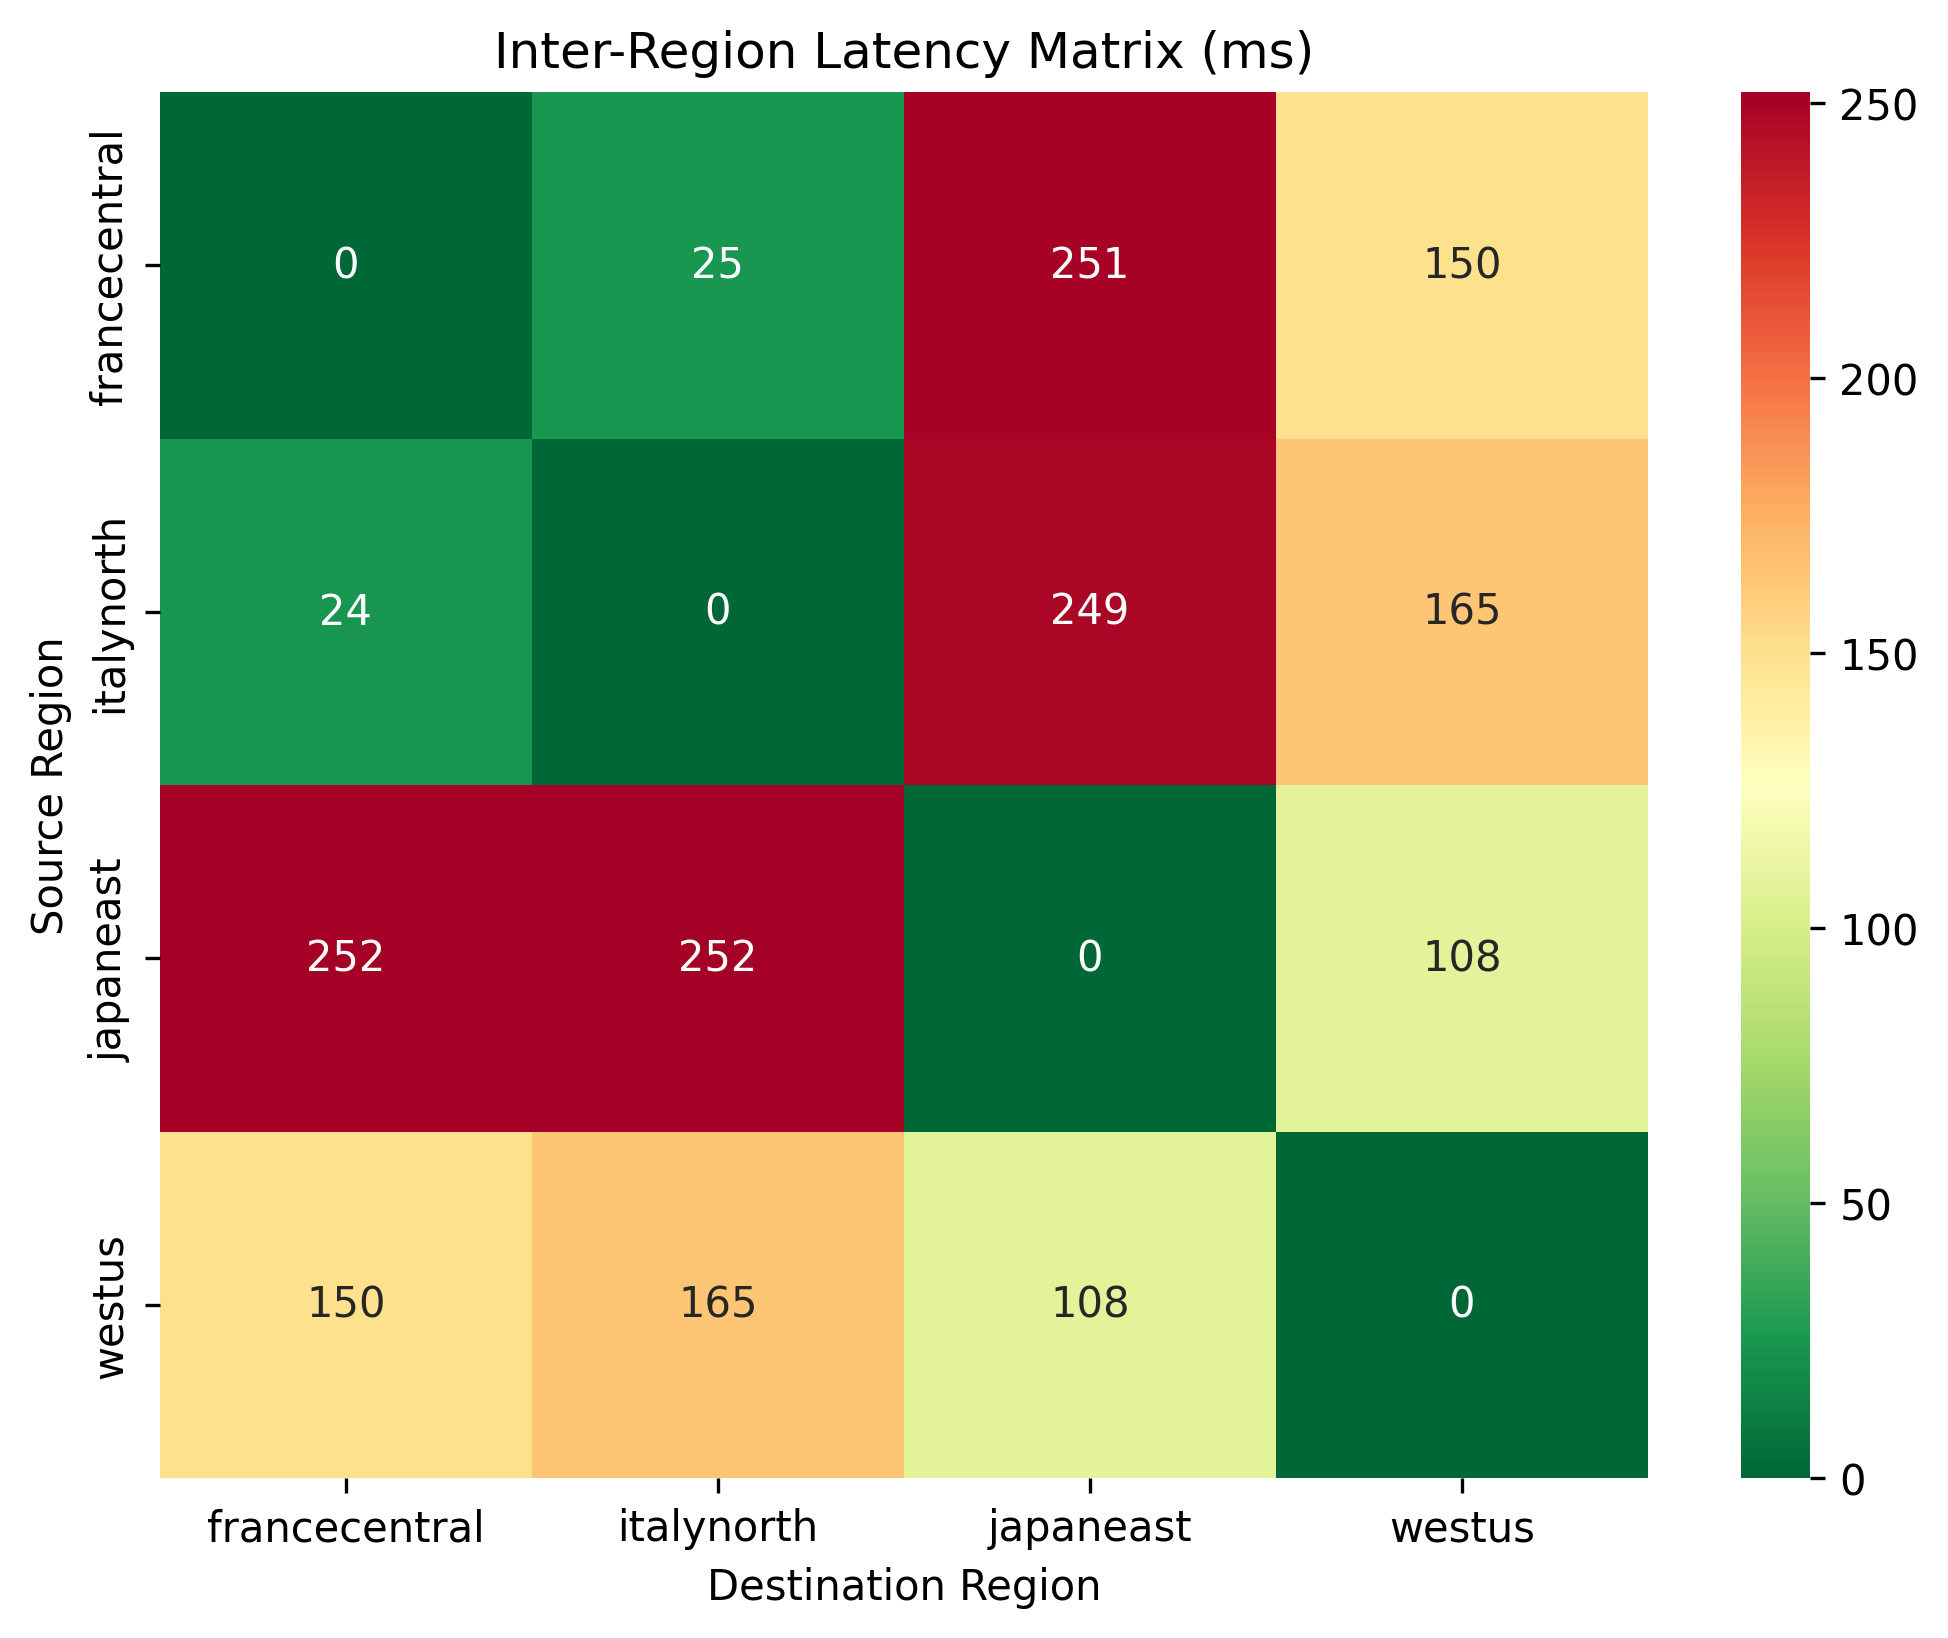
\includegraphics[width=0.75\linewidth]{images/latency_heatmap.png}
  \caption{Latency matrix example (Azure regions subset)}
  \label{fig:latency_matrix}
\end{figure}


\lstset{style=jsonstyle}
\begin{lstlisting}[caption={Latancy matrix example encoded in JSON format}, label={lst:latency_matrix_example}]
  {
    "italynorth": {
        "italynorth": 0,
        "japaneast": 249,
        "francecentral": 24,
        "westus": 165
    },
    "japaneast": {
        "italynorth": 252,
        "japaneast": 0,
        "francecentral": 252,
        "westus": 108
    },
    "francecentral": {
        "italynorth": 25,
        "japaneast": 251,
        "francecentral": 0,
        "westus": 150
    },
    "westus": {
        "italynorth": 165,
        "japaneast": 108,
        "francecentral": 150,
        "westus": 0
    }
}

\end{lstlisting}


data

Azure provides monthly Percentile P50 round trip times between Azure regions:
(https://learn.microsoft.com/en-us/azure/networking/azure-network-latency?tabs=Americas%2CWestUS)
https://learn.microsoft.com/en-us/azure/networking/media/azure-network-latency/azure-network-latency-thumb.png#lightbox 

Azure network latencies docs:
https://raw.githubusercontent.com/MicrosoftDocs/azure-docs/refs/heads/main/articles/networking/azure-network-latency.md

Merged Azure network latencies:
https://docs.google.com/spreadsheets/d/1kxtPw9ZSnAv1vQ6IDwzw-mXdHoKUFb8AjlsjACnvDqE/edit?usp=sharing 


AWS:
https://www.cloudping.co/grid (not official, not using VMs but Lambda functions)
how it is calculated

google
syntetic data
no offical data



\subsection{GDPR policy}

Another policy configured in the system is the ``GDPR Policy'', which ensures that virtual machines (VMs) are deployed in cloud regions that reside in countries of the European Union. 
The policy is based on the principle of \textbf{set intersection}. One set consists of the eligible regions determined by other constraints, such as latency requirements. The other set includes cloud provider regions that are physically located within European Union (EU) countries.
The intersection of these two sets defines the final list of allowed deployment regions, restricting workloads to EU-based data centers.
Since each cloud provider has its own regional distribution, the list of EU-compliant regions is provider-specific and is encoded as contextual data in JSON format. This allows for flexibility and easy updates when cloud providers introduce new regions.

It must be noted that this policy is \textbf{not intended to be a comprehensive GDPR compliance solution}, but rather a basic example of how OPA can enforce \textbf{data residency requirements in a multi-cloud environment}. Organizations with more stringent GDPR compliance needs should consider additional measures.

\subsection{Scheduling outcome policy}

main policy

Mutation policy
dedicated to 



JSON Patch is a format for describing changes to a JSON document which avoid the need to send the entire document when only a part of it has changed. Effectively, only deltas are sent back to the requester which are themselves JSON documents.
The format is defined in RFC 6902 from the IETF \cite{json_patch}.

As an example, a single patch operation 


OPA, assuming the role of a webhook server, has the duty of ..





\subsection{OPA Data mapping}

OPA is flexible enough to handle data mapping between different data models, enabling seamless integration with external systems. In our GreenOps system, data mapping is essential for translating between ElectricityMaps regions and cloud provider regions. 


At some point in the system this mapping needs to be done.
this mappings are needed since the scheudler knows only about ElectricityMaps regions, and do not possess the knowledge of cloud provider regions. Therefore, a mapping is needed to translate the ElectricityMaps regions to cloud provider regions and vice versa.

inside the policy is a good place to do this mapping


first filter is the selection of the provider
this determine the whole set of regions belonging to that provider

eligible regions: this filter can be only done with cloud provider specific latencies

\begin{figure}[H]
  \centering
  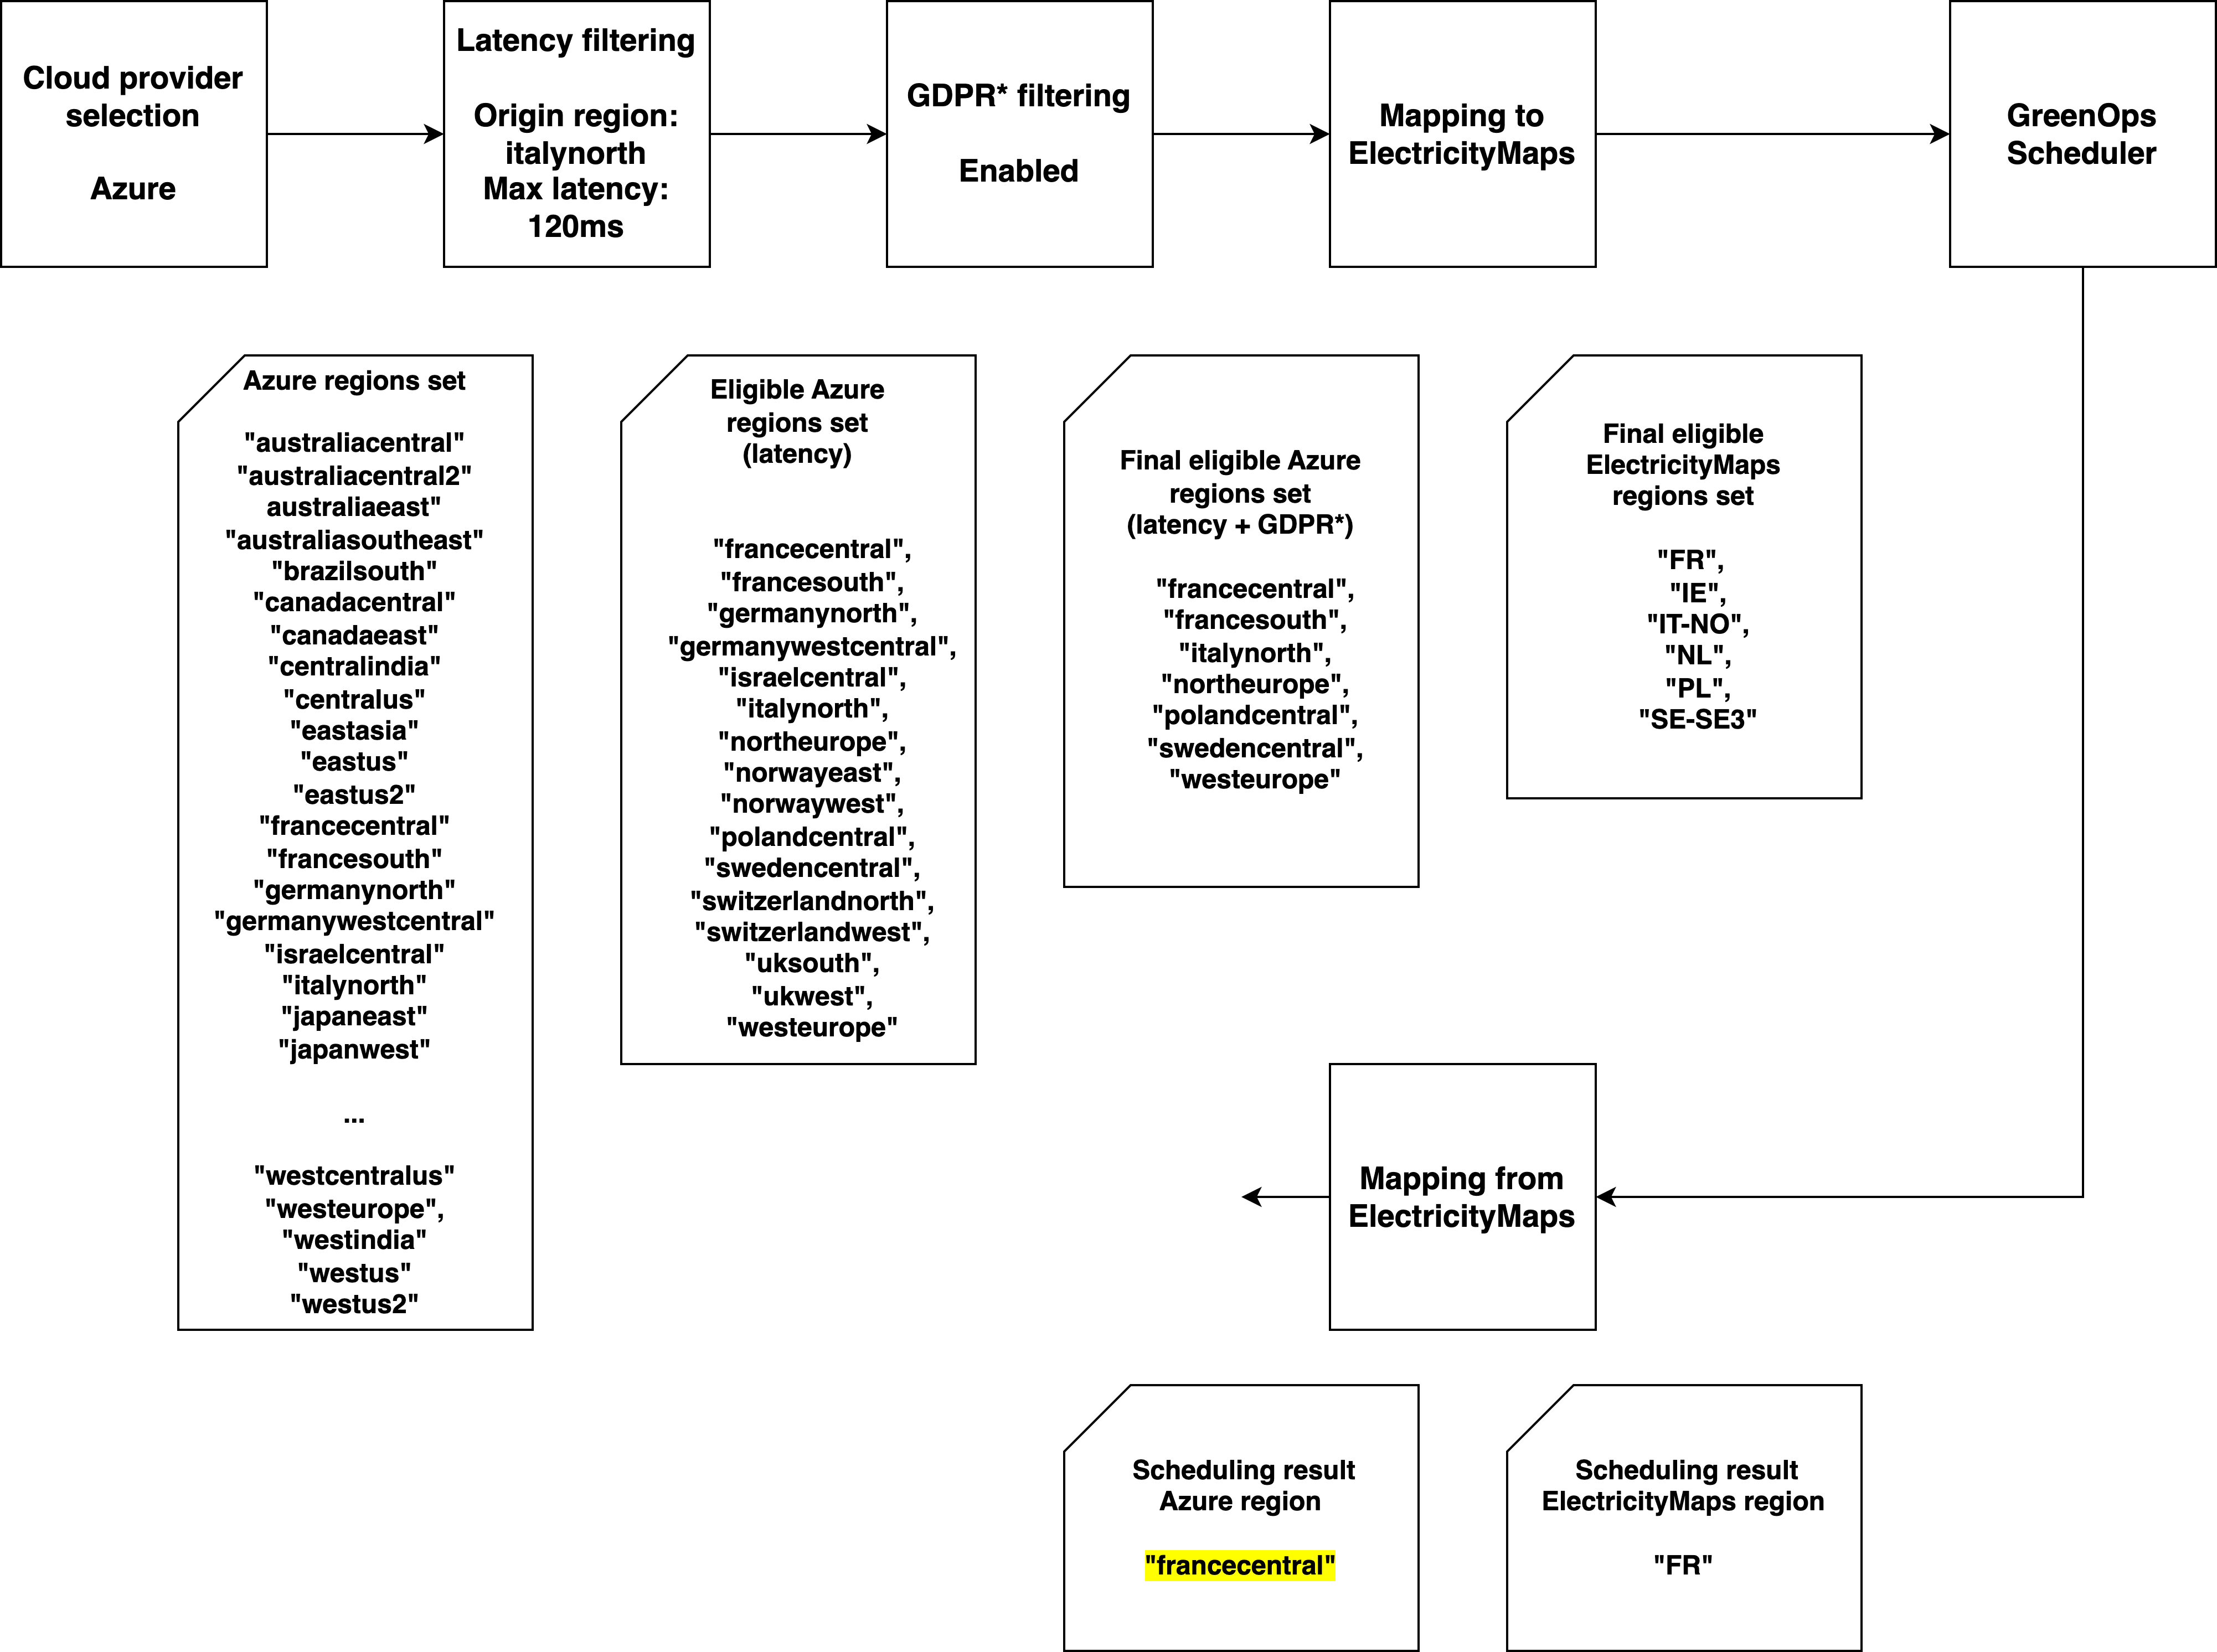
\includegraphics[width=1\linewidth]{images/data_mapping.png}
  \caption{OPA Data mapping}
  \label{fig:data_mapping}
\end{figure}


\begin{lstlisting}[language=Rego, caption=Rego data mapping, label=lst:rego_data_mapping]
# Utility functions to map between cloud provider regions 
# and ElectricityMaps regions

map_to_electricitymaps(eligible_regions, provider) = em_regions if {
    em_regions := {
        region.ElectricityMapsName |                             
        some eligible_region;                       
        some region;                                
        eligible_region = eligible_regions[_];      
        region = data[provider].cloud_regions[_];   
        region.Name == eligible_region             
        region.ElectricityMapsName != ""            
        region.ElectricityMapsName != "Unknown"
    }
}

map_from_electricitymaps(em_region, provider) = cloud_region if {
    some region;                              
    region = data[provider].cloud_regions[_];   
    region.ElectricityMapsName == em_region;    
    cloud_region := region.Name 
}

\end{lstlisting}

\subsection{OPA end-to-end workflow}

 (K8s mutating webhook)

OPA flow:

- admission review (contains max\_latency, origin\_region)

- policy contains cloud provider (or chose for the user)

- policy calculate subset of eligible regions

- policy will ask scheduling information to the scheduler (using http.send()










relationship with k8s mutating webhook

rego policies


scheduler has notions of 
electricity maps regions only

OPA is used also as a data mapping layer
both at request time
and at response time


\begin{figure}[htb]
\centering
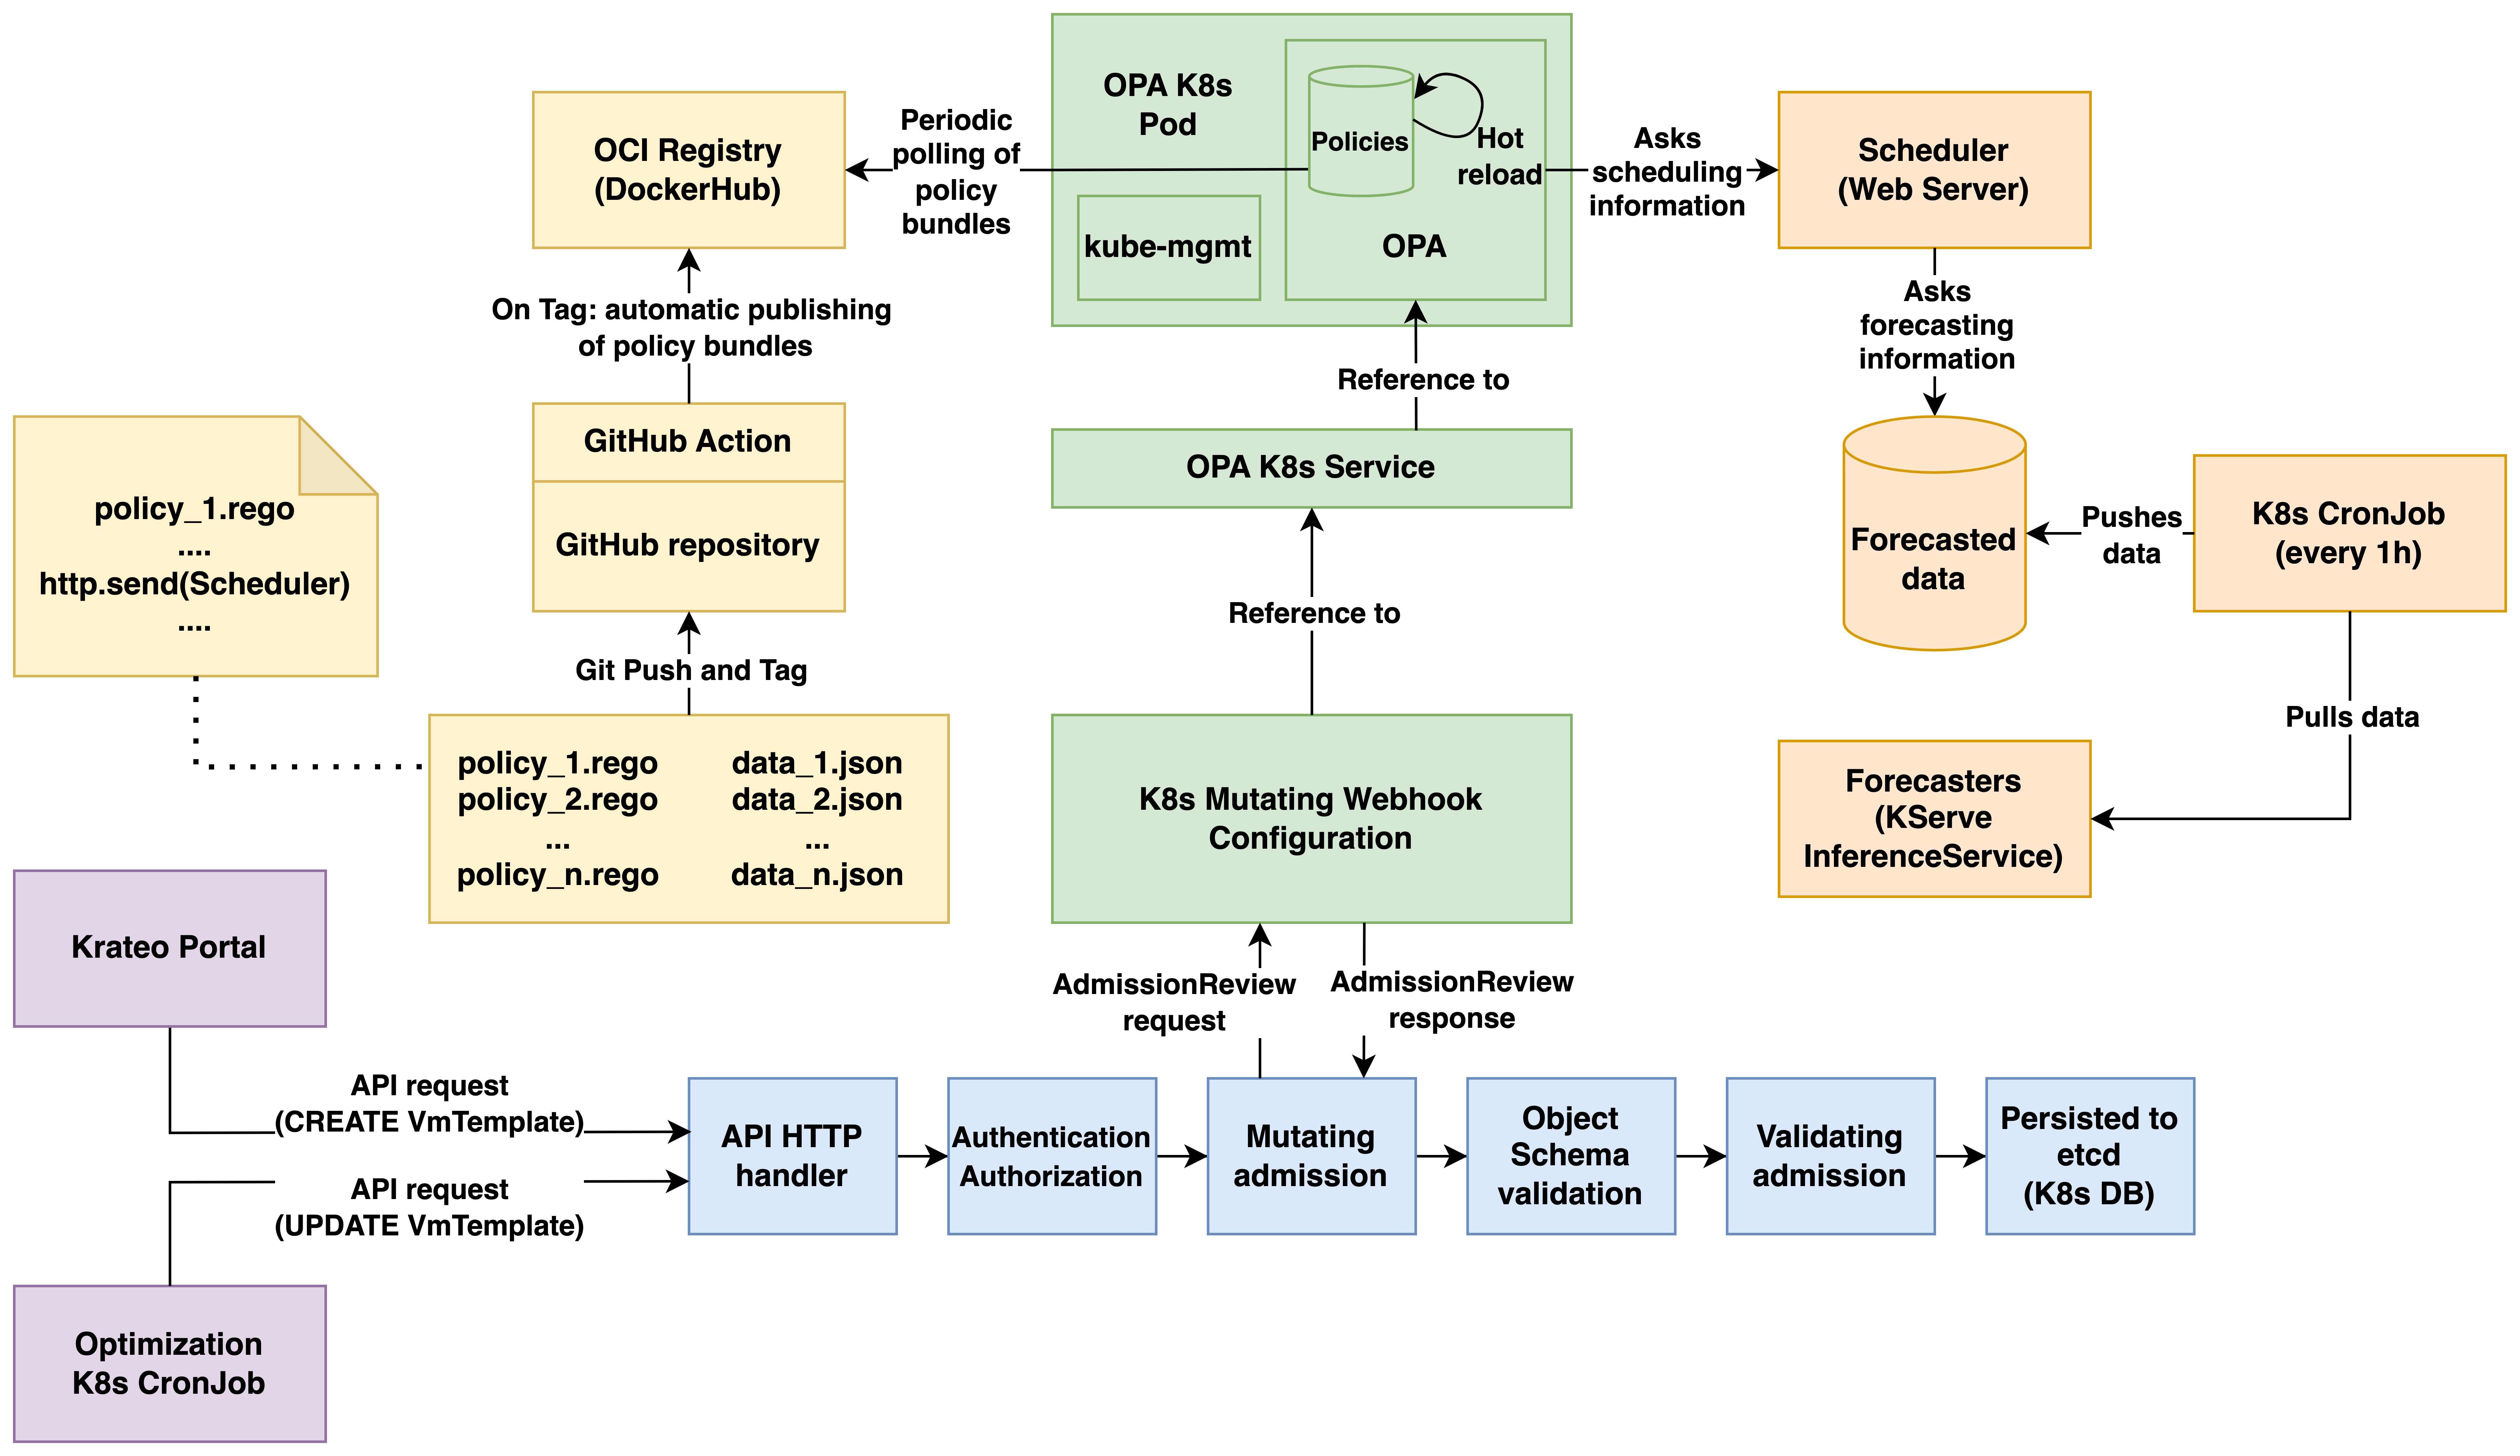
\includegraphics[width=1\linewidth]{images/mutating_webhook+OPA_integration.png}
\caption{Kubernetes mutating webhook + OPA integration}
\label{fig:webhook+opa}
\end{figure}

Figure \ref{fig:webhook+opa} represents the configuration of the Kubernetes Mutating Webhook with the intergeation of Open Policy Agent.
In particular, 




Day 2 operations
what are day 2 operations: in this case (VMs) resize a VM (scale up or down) based on the load
The mutating webhook configuration is set on the CREATE and UPDATE operations

UPDATE operation trigger
K8s Cronjob that attach a label to the custom resoruce 

\subsection{OPA advanced features}

It is deemed useful to mention some of the advanced features of OPA that were not employed in the system described in this thesis but could be potentially useful in future developments or in other contexts where OPA is used.

- bundle signing
- delta bundles

\newpage

\section{MLOps infrastructure}

A MLOps infrastrcutrue is not necessarily needed for multi-cloud resource management but since it is believed that AI models will be used in the future more and more to get scheduling and management decisions
as testified by recents works described in chapter XXX.
It is therefore deemed important to describe a MLOps infrastructure in a Kubernetes environment leveraged by the system described in this thesis.

\subsection{MLOps purpose}

MLOps implements DevOps principles, tools and practices into Machine Learning workflows 

purpose: industrialize ML models lifecycle
faster model development
faster model selection and deployment to production

\begin{itemize}[itemsep=0.2pt, topsep=1pt]
  \item[$\bullet$] model tracking (experiments, runs)
  \item[$\bullet$] model selection (model registry)
  \item[$\bullet$] model storage (in buckets)
  \item[$\bullet$] model deployment (inference)
\end{itemize}


allows all the team member to have visibility on the status of the ML models

Instead of having the so-called ``AI Inference Mock Server", treated as a black box returning a scheul;ding time and schedulingLocation

\begin{figure}[htb]
\centering
\includegraphics[width=1\linewidth]{images/mlops_workflow.png}
\caption{MLOps Architecture}
\label{fig:mlops}
\end{figure}


MLFlow framework
KServe framework


\subsection{MLflow}



MLflow Tracking Server


mlflow is compatible with many ML frameworks like sklearn, pythorch


what is a model tracking server
what is a model registry



Mlflow API calls
autolog function
infer signature 
important since store 

the end result is a self contained fodler with everythiong needed to deploy the model
it allows reproducibility 

The training script will also serialise our trained model, leveraging the MLflow Model format.


model/
├── MLmodel
├── model.pkl
├── conda.yaml
└── requirements.tx


additional challenge: CrateDB is not supported natively by mlflow framework
a CrateDB adapter / wrapper is devoloped and mantianed by cratedb community
CrateDB as metadata stoere


SeaweedFS as artifact store
MINio could be an alternative altough it has a restrictive license \cite{minio_license}.



MODEL signature




\subsubsection{Alternative configuration 1}

an alternative solution

watchdog
watchdog (pyhton package)

sidecar container

artifact store not needed

\subsubsection{Alternative configuration 2}

Another possible configuration could be the adoption of just CrateDB as both Metadata Store and Artifact Store.

This would be possible if
CrateDB supports blob storage but not object storage

This solution cannot be implemented yet due to 


\subsection{KServe}


KServe Inference Service

what is
inference server / model server


used to deploy the forecaster (ML model)


uses Istio and Knative under the hood
features: scaling to zero, etc


InferenceService with TorchServe runtime which is the default installed serving runtime for PyTorch models.

Kserve project proposes a standard protocol for inference servers.
The version 2 of the KServe Inference Protocol is the Open Inference Protocol.



\subsubsection{Open Inference Protocol}


\begin{table}[h!]
\centering
\begin{tabular}{|l|l|l|}
\hline
\textbf{API}    & \textbf{Verb} & \textbf{Path}                                                                                         \\ \hline
Inference       & POST          & v2/models/{[}/versions/\textless{}model\_version\textgreater{}{]}/infer                               \\ \hline
Model Ready     & GET           & v2/models/\textless{}model\_name\textgreater{}{[}/versions/{]}/ready                                  \\ \hline
Model Metadata  & GET           & v2/models/\textless{}model\_name\textgreater{}{[}/versions/\textless{}model\_version\textgreater{}{]} \\ \hline
Server Ready    & GET           & v2/health/ready                                                                                       \\ \hline
Server Live     & GET           & v2/health/live                                                                                        \\ \hline
Server Metadata & GET           & v2                                                                                                    \\ \hline
\end{tabular}
\end{table}





adopted by NVIDIA



multi model deployment



our strategy:
1 model per region
1 generic model? as fallback if specific model is not available?




Kserve "stack"

Kserve

in kserve 0.14.1
clusterservingruntimes
supported are 10
among which 
torchserve

clusterservingruntimes -> kserve-mlserver (supported models: sklearn, xgboost, lightgbm, mlflow)

mlserver

[chart to illustrate this]







serving runtimes

Seldon MLserver


accorgimenti: \\
model wrapping

\section{Measurements}


\subsection{System / performance metrics}


how to measuere cloud resource systems


especially useful for ``day 2 operations''
scaling down a VM


Metrics collected could be:
CPU usage
memory usage.
These metrics are especially useful for the 2nd use case for instance: scaling down a VM.


Prometheus exporters (https://prometheus.io/docs/instrumenting/exporters/) + Prometheus scrapers for data collection.
Generic Prometheus exporters and scrapers already used for Krateo Composable FinOps leveraging specific K8s Custom Resources. These exporters are generic and can scrape arbitrary metrics configured in specific CRs (for instance, collecting VMs CPU consumption though Azure APIs).
From the Krateo Composable FinOps document: 
- “we transform all optimizations into a set of Kubernetes Custom Resources (CRs) to act upon newly found cost-related deficiencies. This allows us to use Kubernetes operators (explicitly coded to interact with cloud services) to monitor these metrics and act automatically to apply changes to remote resources.”

- “forward the optimization to the Krateo operator that manages the services that need to be optimized, for example, the Azure Operator to modify the size of a Virtual Machine;”

- “the optimization is automatically encoded in a CR for the finops-operator-vm-manager, which then analyzes it and decides how to manage the Virtual Machine. For example, it could scale up or down the virtual machine, stop it for the night, etc.”

From my current understanding, only Azure is available for now on the finops-operator-vm-manager. 
This operator is only able to: start; stop; deallocate; scale-up; scale-down.
So finops-operator-vm-manager operates on already provisioned virtual machines and it applies optimizations.

---



Cloud providers API (“hypervisor” / host level) to get CPU usage, memory usage
Azure monitoring REST API: https://learn.microsoft.com/en-us/azure/azure-monitor/essentials/rest-api-walkthrough?tabs=rest%2Cportal
https://learn.microsoft.com/en-us/rest/api/monitor/metrics/list?view=rest-monitor-2023-10-01&tabs=HTTP
https://learn.microsoft.com/en-us/azure/virtual-machines/monitor-vm 


Cloud providers agents
Azure Monitor Agent (https://learn.microsoft.com/en-us/azure/azure-monitor/agents/azure-monitor-agent-overview)
Google Ops Agent: “the primary agent for collecting telemetry from your Compute Engine instances” (https://cloud.google.com/monitoring/agent/ops-agent)


Standard agents/deamons manually installed the VMs (e.g. Prometheus node exporter, 
many metrics restricted by public cloud providers
not straightforward to automate the deployment


---

Challenges
Public Cloud Providers do not provide data about carbon intensity of a VM instance
Public Cloud Providers do not provide data about power consumption of a VM instance

Power consumption metrics
scaphandre: NOT supported by public cloud providers. “Public cloud providers do not expose the underlying RAPL sensors that scaphandre and other measurement tools rely on to track consumption”. (https://github.com/hubblo-org/scaphandre/issues/142)
https://hubblo-org.github.io/scaphandre-documentation/index.html

kepler: really interesting and quite mature project but works only with K8s resources inside the cluster (Nodes, Pods). Therefore not good for our use first case.
https://sustainable-computing.io/design/architecture/


manually estimate power consumption based on CPU utilization, memory usage. Could be a very difficult task. 
there is the TEADS metodology like 



---


Carbon metrics:
there is no adopted standard, there is not something similar to FOCUS yet;
there is a proposal for a specification (work in progress, not supported yet by Public Cloud Providers): 
https://github.com/Green-Software-Foundation/real-time-cloud 
https://github.com/Green-Software-Foundation/real-time-cloud/blob/main/Cloud_Region_Metadata_specification.md 


Public Cloud Providers monthly reports (probably not useful in this case)
Export Azure carbon optimization emissions data (Preview) (probably not fine-grained as we want)

Cloud Carbon Footprint
Uses cloud provider billing (AWS Cost and Usage Reports with Amazon Athena, GCP Billing Export Table using BigQuery, Azure Consumption 
Management API). Using these services costs.
Electricity Maps API integration is supported (for live grid carbon intensity)

 
aether calculation engine (https://aether.green/docs/methodologies/) 
only AWS and GCP supported, Azure not yet
uses AWS CloudWatch and Google monitoring
very small project
no live Grid Carbon Intensity Coefficient, they extrapolate data from “governative” data reports
https://aether.green/docs/methodologies/#grid-carbon-intensity-coefficient


carbond agent) (https://gitlab.com/sustainable-computing-systems/carbond)
installed on the machine


Example of a manual approach (not scalable due to tech specs research): https://devblogs.microsoft.com/sustainable-software/how-can-i-calculate-co2eq-emissions-for-my-azure-vm/ 

The critical point here is to get/calculate the energy consumed by a cloud instance, since there are a huge number of technical configurations to find, retrieve and use for calculations.



\subsection{Impact framework}

Impact framework (by green software foundation)

\section{End-to-End workflow}
\label{sec:e2eflow}

[TO BE CHANGED]
A user request for a workload arrives in Kubernetes / Krateo. 
The request shape is VM1 = (MinCPU=4vCPU, MinRAM=4GiB, D=12h)
As we can see the request is generic: it does not contain a specific cloud provider or a specific cloud region.
A K8s Custom Resource (CR) representing the workload is created.
mutating webhook intercepts the CREATE API request.
K8s mutating webhook retrieve and evaluate policies and in particular, the AI model inference is called and should return a decision with the region and scheduling time (time-shifting and geographical shifting).
OPA will use this decision to mutate the VM specification, adding the provider, the schedulingRegion and schedulingTime fields.
Krateo core provider / cdc


\begin{sidewaysfigure}
  \centering
  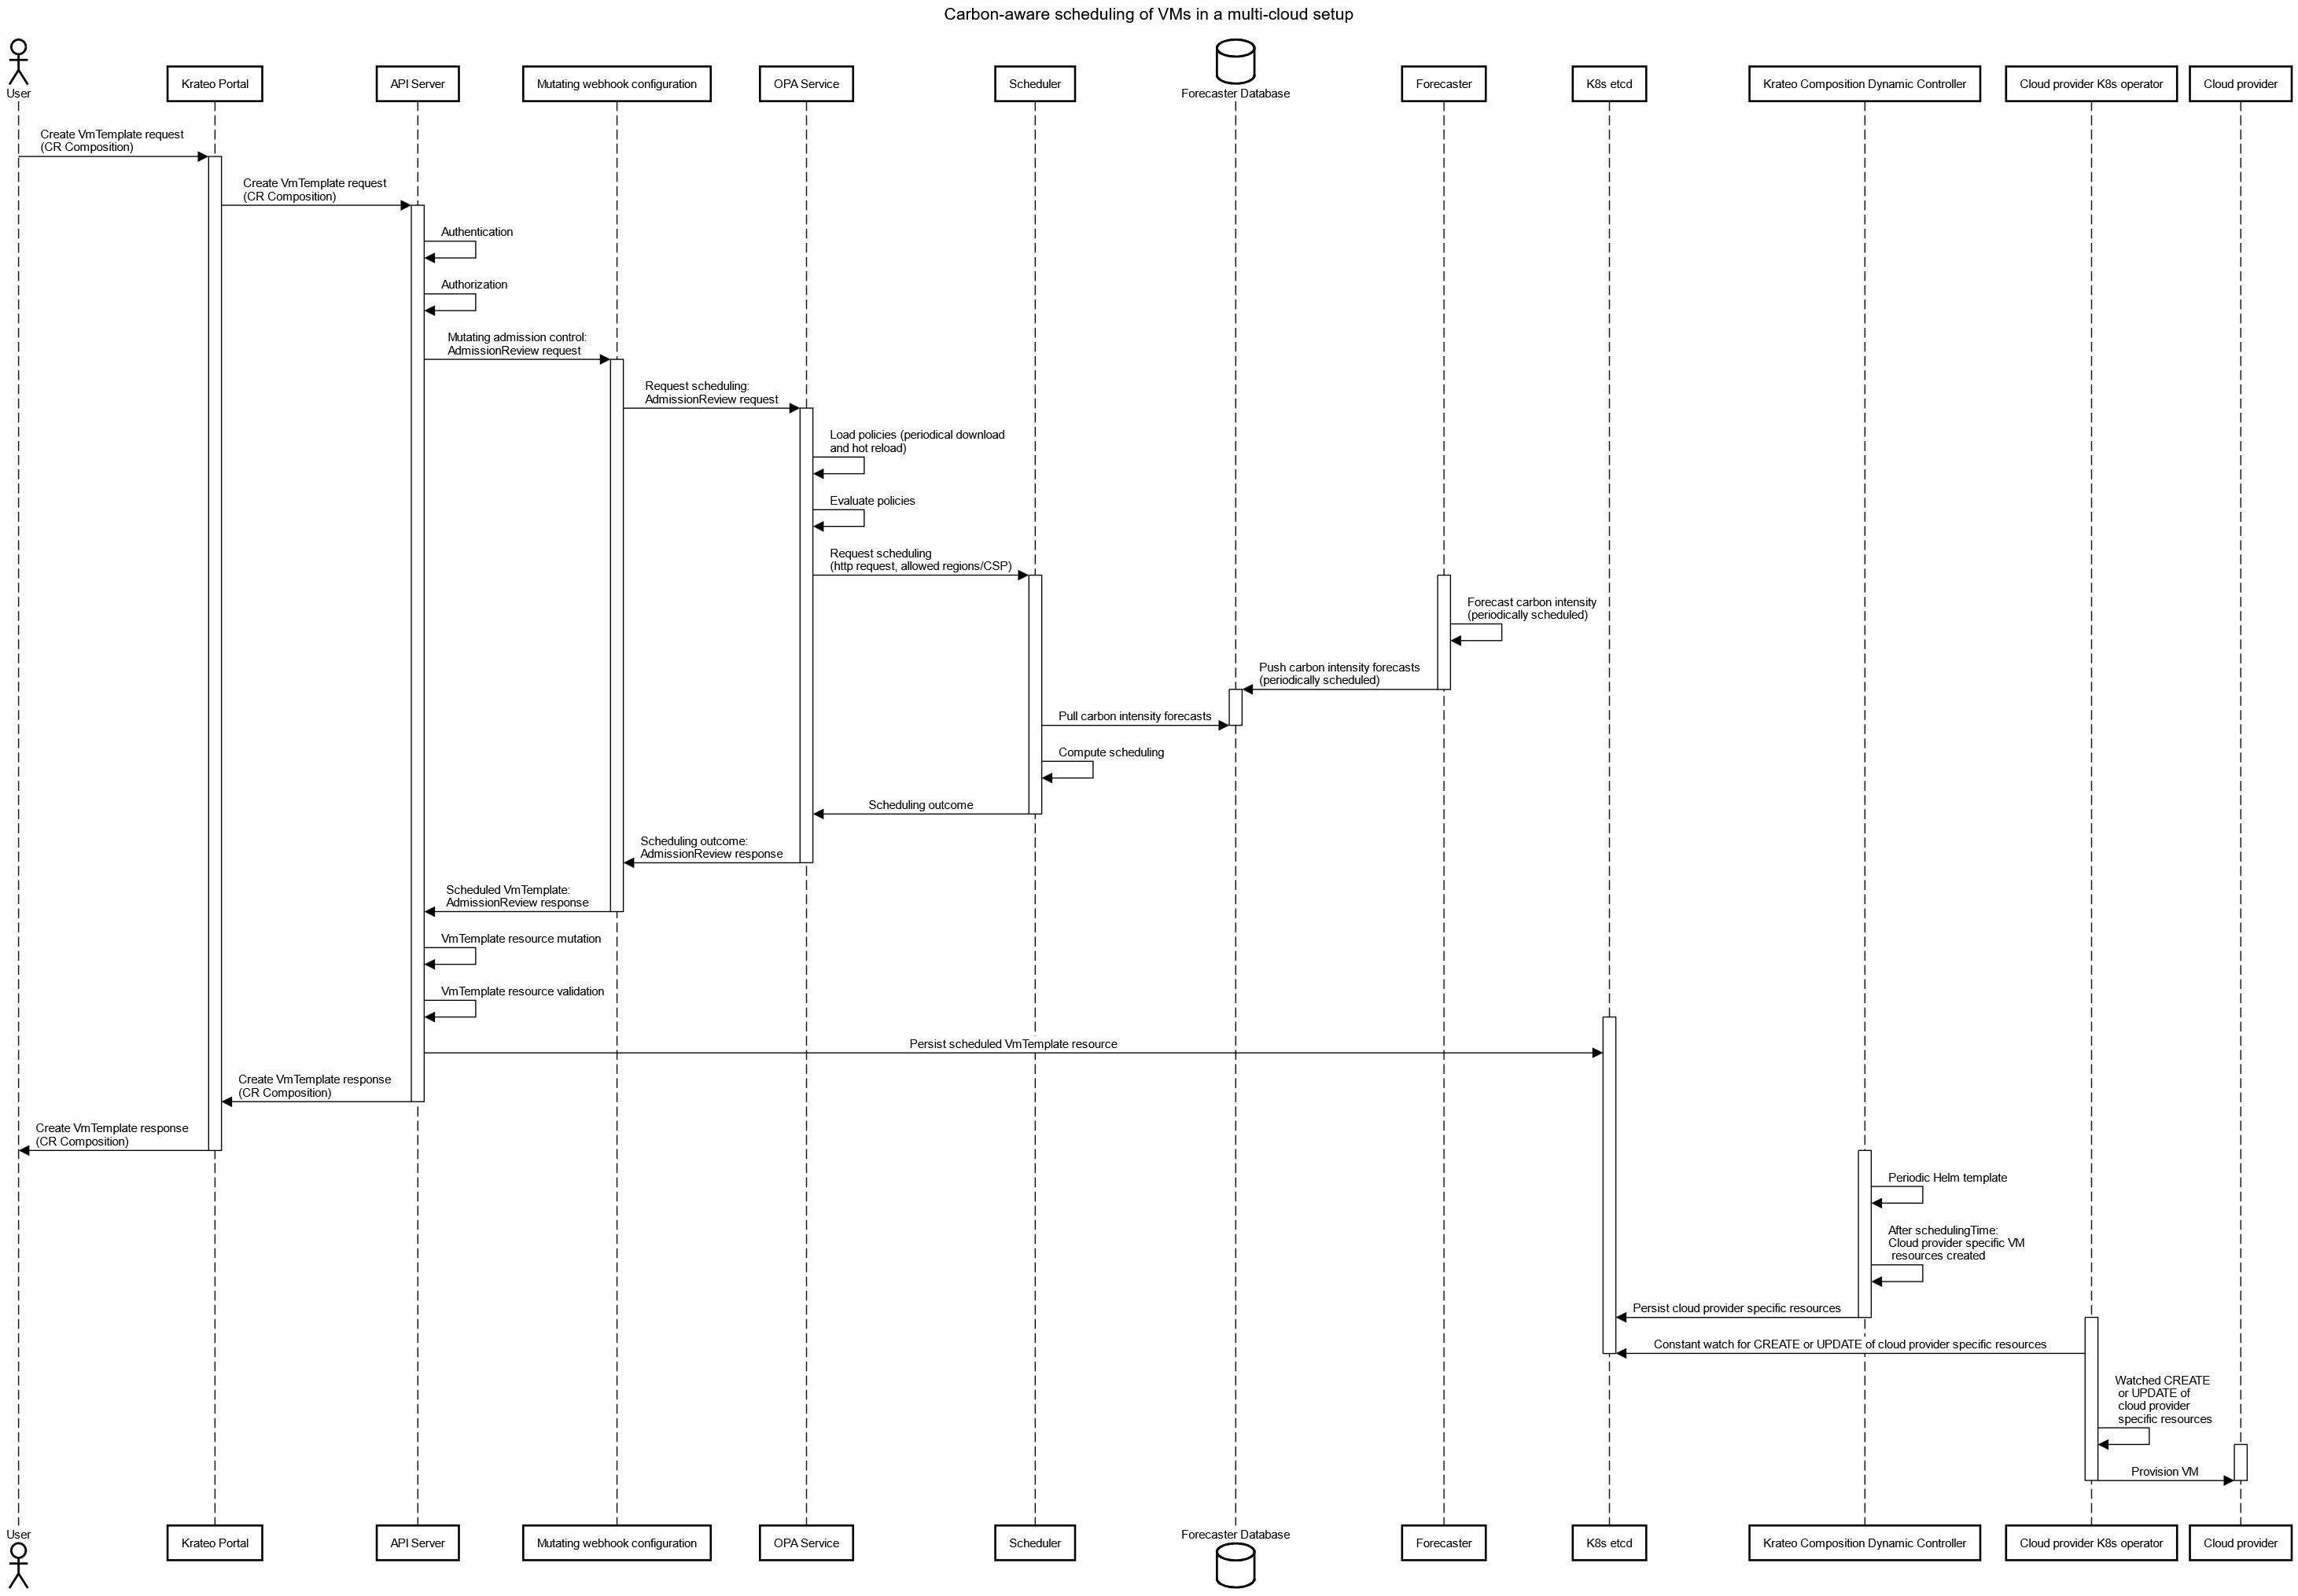
\includegraphics[width=\textheight]{images/sequence_diagram.png}
  \caption{Example of a full-page rotated image}
  \label{fig:rotated_image}
\end{sidewaysfigure}


\newpage







Table for recap of all tools used

Kubernetes
- Krateo
Helm
    Helm charts
    Helm templating
    Helm lookup function

- VmTemplate Krateo Composition Definition
- Azure K8s Operator
- GCP K8s Operator
- AWS K8s Operator
- K8s mutating webhook configuration
- OPA server
- opa policies
- OPA bundles
- MLflow tracking server (+ metadata store & artifact store)
- Forecaster (deployed as KServe InferenceService)


\newpage

      \chapter{Design and Implementation}
\label{cha:design}

This chapter presents the design and implementation of our system, focusing on the integration of the various components and the overall architecture. The system is designed to be modular, scalable, and extensible, enabling the integration of additional components as needed.

\section{Assumptions}



\subsection{workload definition}
In this work, workload has been modeled as \textbf{Virtual Machines (VMs)}, representing the primary use case considered during the system's initial design phase. 
[WHY THIS CHOICE?]

We define, for the purpose of this work, a workload as a Virtual Machine (VM).
We can assume/imagine that inside of the VM, some kind of processing/work P will happen.
This VM can be scheduled on any Public Cloud Provider since we are looking for a multi-cloud setting: cloud can be seen as a commodity. 
Alternatively, a subset of eligible Public Cloud Providers can be set as a policy.
We can use general-purpose VMs.

The VM has the following characteristics:
MinCPU needed
MinRAM needed
Duration (D): the time duration that a VM must run to accomplish its processing/work
Deadline (DL): the time (timestamp) when the VM must have finish its work (maybe this can be omitted for the basic use cases)
Max latency (ML): value in ms 

If the workload is completely delay-tolerant then the Deadline parameter must not be used.

So a VM could be defined as a tuple like the following:
VM = (MinCPU, MinRAM, D, DL, ML)


example

Min CPU: 4 vCPU
Min RAM: 4 GB of RAM
Duration (D): 1h
Deadline (DL): 2022-12-31 23:59:59
---

The system is designed to be cloud-agnostic, however for the purpose of this work, the system is currently configured to support three major cloud providers: \textbf{Microsoft Azure}, \textbf{Google Cloud Platform (GCP)}, and \textbf{Amazon Web Services (AWS)}.

---






A limitation of our general approach is that only resources supported by the cloud provider’s Kubernetes operator can be provisioned. Not all cloud resources available in a provider’s portfolio are guaranteed to have corresponding Kubernetes Custom Resources (CRs). This introduces certain constraints:

\begin{itemize}[itemsep=0.2pt, topsep=1pt]
  \item[$\bullet$] Limited resource availability: if a specific resource type (e.g., a GPU-accelerated instance or a managed database service) is not supported by the cloud provider Operator, it cannot be provisioned using the current system.
  \item[$\bullet$] Dependence on Operator updates: cloud providers may extend or modify the set of resources supported by their Kubernetes operators over time.
  \item[$\bullet$] Vendor-specific implementations: different cloud providers expose varying levels of support for Kubernetes-native resource provisioning, leading to potential inconsistencies across multi-cloud environments.
\end{itemize}

Despite these constraints, the system architecture remains highly adaptable, and future enhancements could incorporate additional or alternative provisioning mechanisms. 
An example of an alternative implementation could be the direct API interactions with cloud providers to bypass operator limitations. Another approach could involve the development of custom operators or controllers to manage specific resource types not supported by existing operators. 
[KRATEO custom operator REST]

\newpage

\section{System Architecture}
\label{sec:system_architecture}

The following table provides an overview of the main components of the system and their respective functions.

\begin{table}[H]
  \centering
  \renewcommand{\arraystretch}{1.3} % Adjust row height for readability
  \begin{tabularx}{\textwidth}{| l | X |} % 'X' makes the second column auto-wrap
    \hline
    \textbf{Component} & \textbf{Function} \\
    \hline
    Krateo PlatformOps & Provides an abstraction layer for infrastructure orchestration, enabling declarative resource management and integration with cloud providers with templates. \\
    \hline
    Cloud Providers Kubernetes Operators & Manages the provisioning and reconciliation of cloud resources within Kubernetes, ensuring the actual state matches the desired state. \\
    \hline
    Kubernetes Mutating Webhook Configuration & Intercepts and modifies API requests before they are persisted, allowing dynamic configuration adjustments with policy enforcement. \\
    \hline
    OPA Server & Evaluates authorization and policy decisions based on defined constraints and input data from Kubernetes API requests through the webhook. \\
    \hline
    OPA Policies and Data & Define the rules and contextual information used by OPA to make policy decisions, namely scheduling information \\
    \hline
    GreenOps Scheduler & Determines the optimal scheduling region and scheduling time for VMs, acting as an external data source for OPA policies. \\
    \hline
    MLflow & Allows the tracking, logging, versioning and storing of machine learning experiments for reproducibility and model lifecycle management. \\
    \hline
    KServe & Provides scalable and Kubernetes-native model serving capabilities, enabling deployment of machine learning models for inference. \\
    \hline
  \end{tabularx}
  \caption{Main components of the system and their respective functions.}
  \label{tab:system_components}
\end{table}

All the components listed in the above table must be deployed inside a Kubernetes cluster. The only exception are the OPA Policies and data which lies outside the cluster as described in section \ref{sec:opa_bundles}.

\section{Krateo PlatformOps integration}

Krateo PlatformOps is utilized in this system for \textbf{multi-cloud resource management}, allowing for the declarative orchestration of cloud resources across different cloud providers leveragin Kubernetes as a control plane. 
This section highlights the differences between two approaches for resource synchronization:
\begin{itemize}[itemsep=0.2pt, topsep=1pt]
  \item[$\bullet$] The \textbf{Custom Kubernetes ``Synchronization Operator"} approach
  \item[$\bullet$] The \textbf{Krateo PlatformOps} approach
\end{itemize}

It is deemed interesting to describe both approaches in order to identify the several trade-offs between implementing a custom synchronization operator and leveraging a template-based abstraction for cloud resource provisioning.

\subsection{Resource management: the Custom Kubernetes ``Synchronization Operator" approach}

When dealing with multi-cloud workloads with Kubernetes as a control plane, a synchronization and mapping mechanism is required to bridge the gap between:
\begin{itemize}[itemsep=0.2pt, topsep=1pt]
  \item[$\bullet$] \textbf{Generic Kubernetes Custom Resources}, which represent generic provider-agnostic workloads.
  \item[$\bullet$] \textbf{Cloud provider-specific Custom Resources}, which correspond to the actual cloud resources provisioned through the respective Kubernetes operators provided by Azure, AWS or GCP (in our case).
\end{itemize}

A custom Kubernetes Operator would be responsible for the mapping and synchronization of the above resource types. This approach is based on the principle of \textbf{Continuous Reconciliation}, where the operator continuously monitors and adjusts the system to maintain consistency between the desired and actual states.
Candidate solutions for the development of the K8s Operator includes: Operator SDK, Kubebuilder, or writing the operator from scratch using the Kubernetes client libraries. For the purpose of this work, Kubebuilder was used to develop a Proof of Concept (PoC) for the custom synchronization operator.

\subsubsection{Responsibilities of the Custom Operator}

In our specific case, the operator should continuously watch the generic CRs in the Kubernetes cluster to check if critical scheduling fields have been set:
\begin{itemize}[itemsep=0.2pt, topsep=1pt]
  \item[$\bullet$] \textbf{schedulingRegion}: Defines where the workload should be placed.
  \item[$\bullet$] \textbf{schedulingTime}: Specifies when the workload should be deployed.
\end{itemize}

These fields, if set, indicate a geographical placement and timing for the workload have been determined by the GreenOps Scheduler.
If these fields are not yet present, the operator must wait for scheduling decisions before proceeding.
Therefore, inside its Reconcile() loop, the operator should:
\begin{enumerate}[itemsep=0.2pt, topsep=1pt]
  \item Continuously check if scheduling fields (schedulingRegion, schedulingTime) are set.
  \item Trigger the creation of the provider-specific resource when the schedulingTime is approaching.
  \item Track the provisioning status by marking the generic CR with a field indicating that the cloud-specific resource has been created.
\end{enumerate}

\subsubsection{Post-Creation Considerations}

Once the cloud provider-specific resource is created, two main questions arise:
\begin{itemize}[itemsep=0.2pt, topsep=1pt]
  \item[$\bullet$] What happens if the provider-specific CR is modified manually?
  \item[$\bullet$] What happens if the VM configuration is modified directly on the cloud provider (outside Kubernetes)?
\end{itemize}

Related to the first question, an example scenario could be: changing the VM instance type (VM size) inside the Kubernetes cluster. In this case, the operator needs to decide whether to revert unauthorized changes or allow them and update the generic CR accordingly.
For the second question, an example could be: changing the VM size directly on the cloud provider’s console. In this case, the operator should detect the drift and update the generic CR to reflect the external changes.

\subsubsection{Resource linking}

A mechanism must be in place to link the generic CR to the cloud provider-specific CR. Possible approaches include:
\begin{itemize}[itemsep=0.2pt, topsep=1pt]
  \item[$\bullet$] UUID-based linking: A universally unique identifier ensuring each resource is mapped correctly.
  \item[$\bullet$] Kubernetes Object Metadata (ObjectMetadata.Name \& ObjectMetadata.Namespace): This approach may be preferable within a single Kubernetes cluster, avoiding the need for an external ID system.
\end{itemize}

\subsubsection{Termination Logic}

The operator must handle the deletion of cloud resources correctly in a variety of scenarios:
\begin{itemize}[itemsep=0.2pt, topsep=1pt]
  \item[$\bullet$] When the provider-specific CR is deleted from Kubernetes, the corresponding cloud resource is de-provisioned and the custom operator should ensure the deletion process is handled gracefully, avoiding orphaned generic CRs.
  \item[$\bullet$] If the provider-specific CR is deleted directly on the cloud provider, the operator should detect the change and update the generic CR accordingly.
  \item[$\bullet$] In the event of a generic CR deletion, the custom operator should ensure the provider specific resource is removed, troggering a deletion process on the cloud provider side (de-provisioning).
\end{itemize}

\subsubsection{Managing cloud provider-specific fields}
Each cloud provider has unique resource configurations and constraints that must be managed.
Some differences are purely syntactic (e.g., AWS uses instanceType, whereas Azure uses vmSize).
Others require additional provider-specific metadata (e.g., Azure requires a resourceGroup field which represent a logical container for resources in Azure).
A custom synchronization operator must encode this logic explicitly, making it more complex to maintain especially when supporting several cloud providers.

\subsubsection{Limitations of a Custom ``Synchronization Operator''}
Another major challenge with a custom synchronization operator is that some cloud providers do not support time scheduling metadata within their Custom Resources. In particular, no cloud operator among the ones we used for the system (AWS, Azure, GCP) provides a dedicated field for scheduling time.
This means that the Kubernetes operator itself must handle time scheduling logic, delaying CR creation until the scheduled time.
If the operator, upon the creation of a generic CR, immediately creates the cloud-provider specific CR (without a ``waiting logic''), the cloud provider Operator will trigger and provision the VM immediately, ignoring scheduling constraints.
Due to these limitations and complexities, we explored and leveraged an \textbf{alternative template-driven approach} using Krateo PlatformOps, described in the next section.

\begin{figure}[htb]
  \centering
  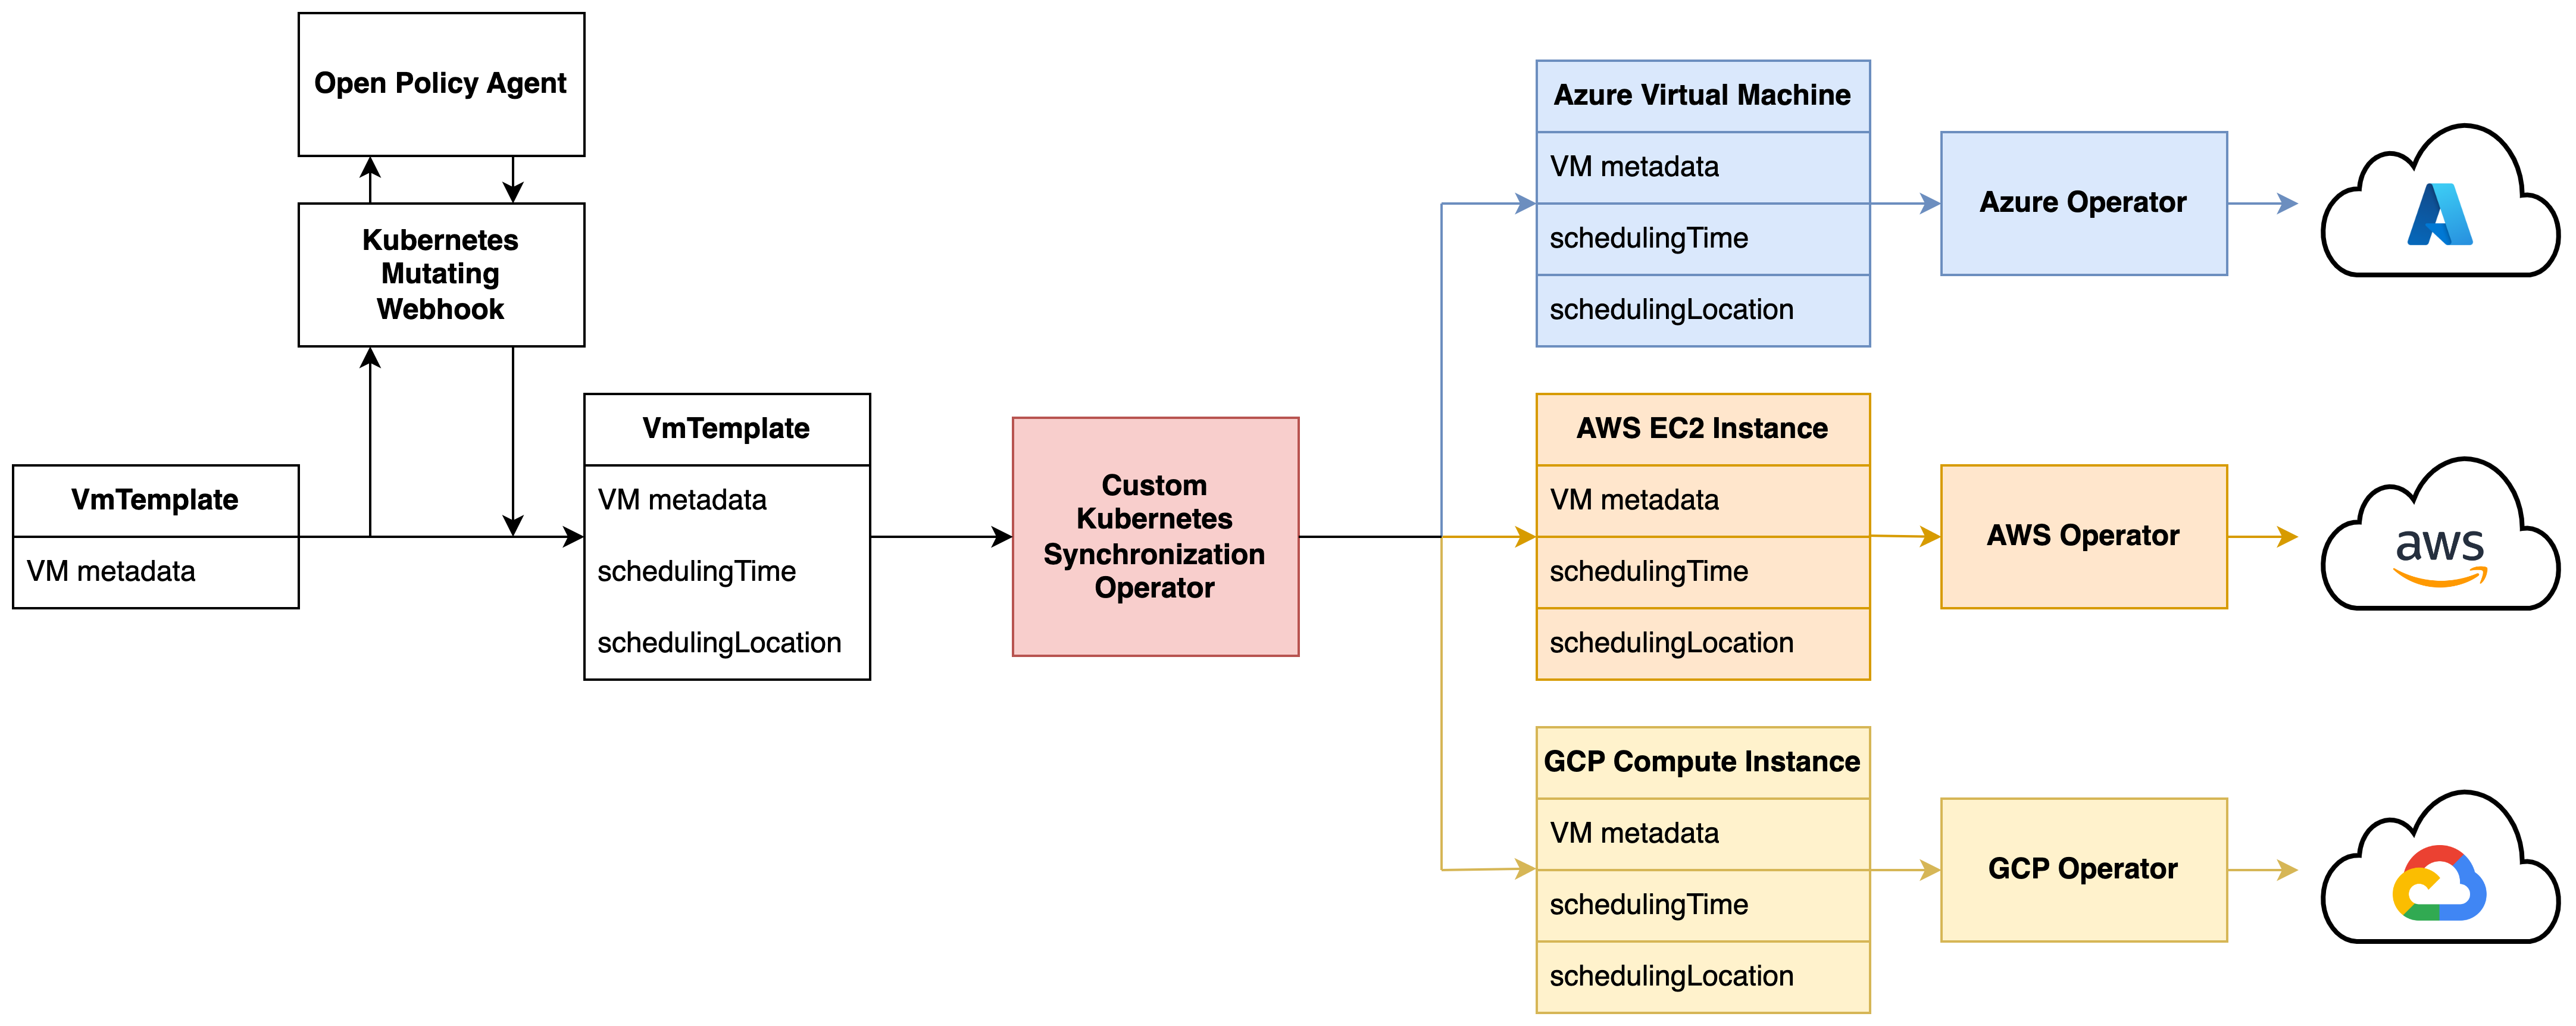
\includegraphics[width=1\linewidth]{images/k8s_operator.png}
  \caption{Multi-cloud resource management with Custom Kubernetes ``Synchronization Operator'' approach}
  \label{fig:k8s_operator}
\end{figure}

\subsection{Resource management: the Krateo approach}

\begin{figure}[htb]
  \centering
  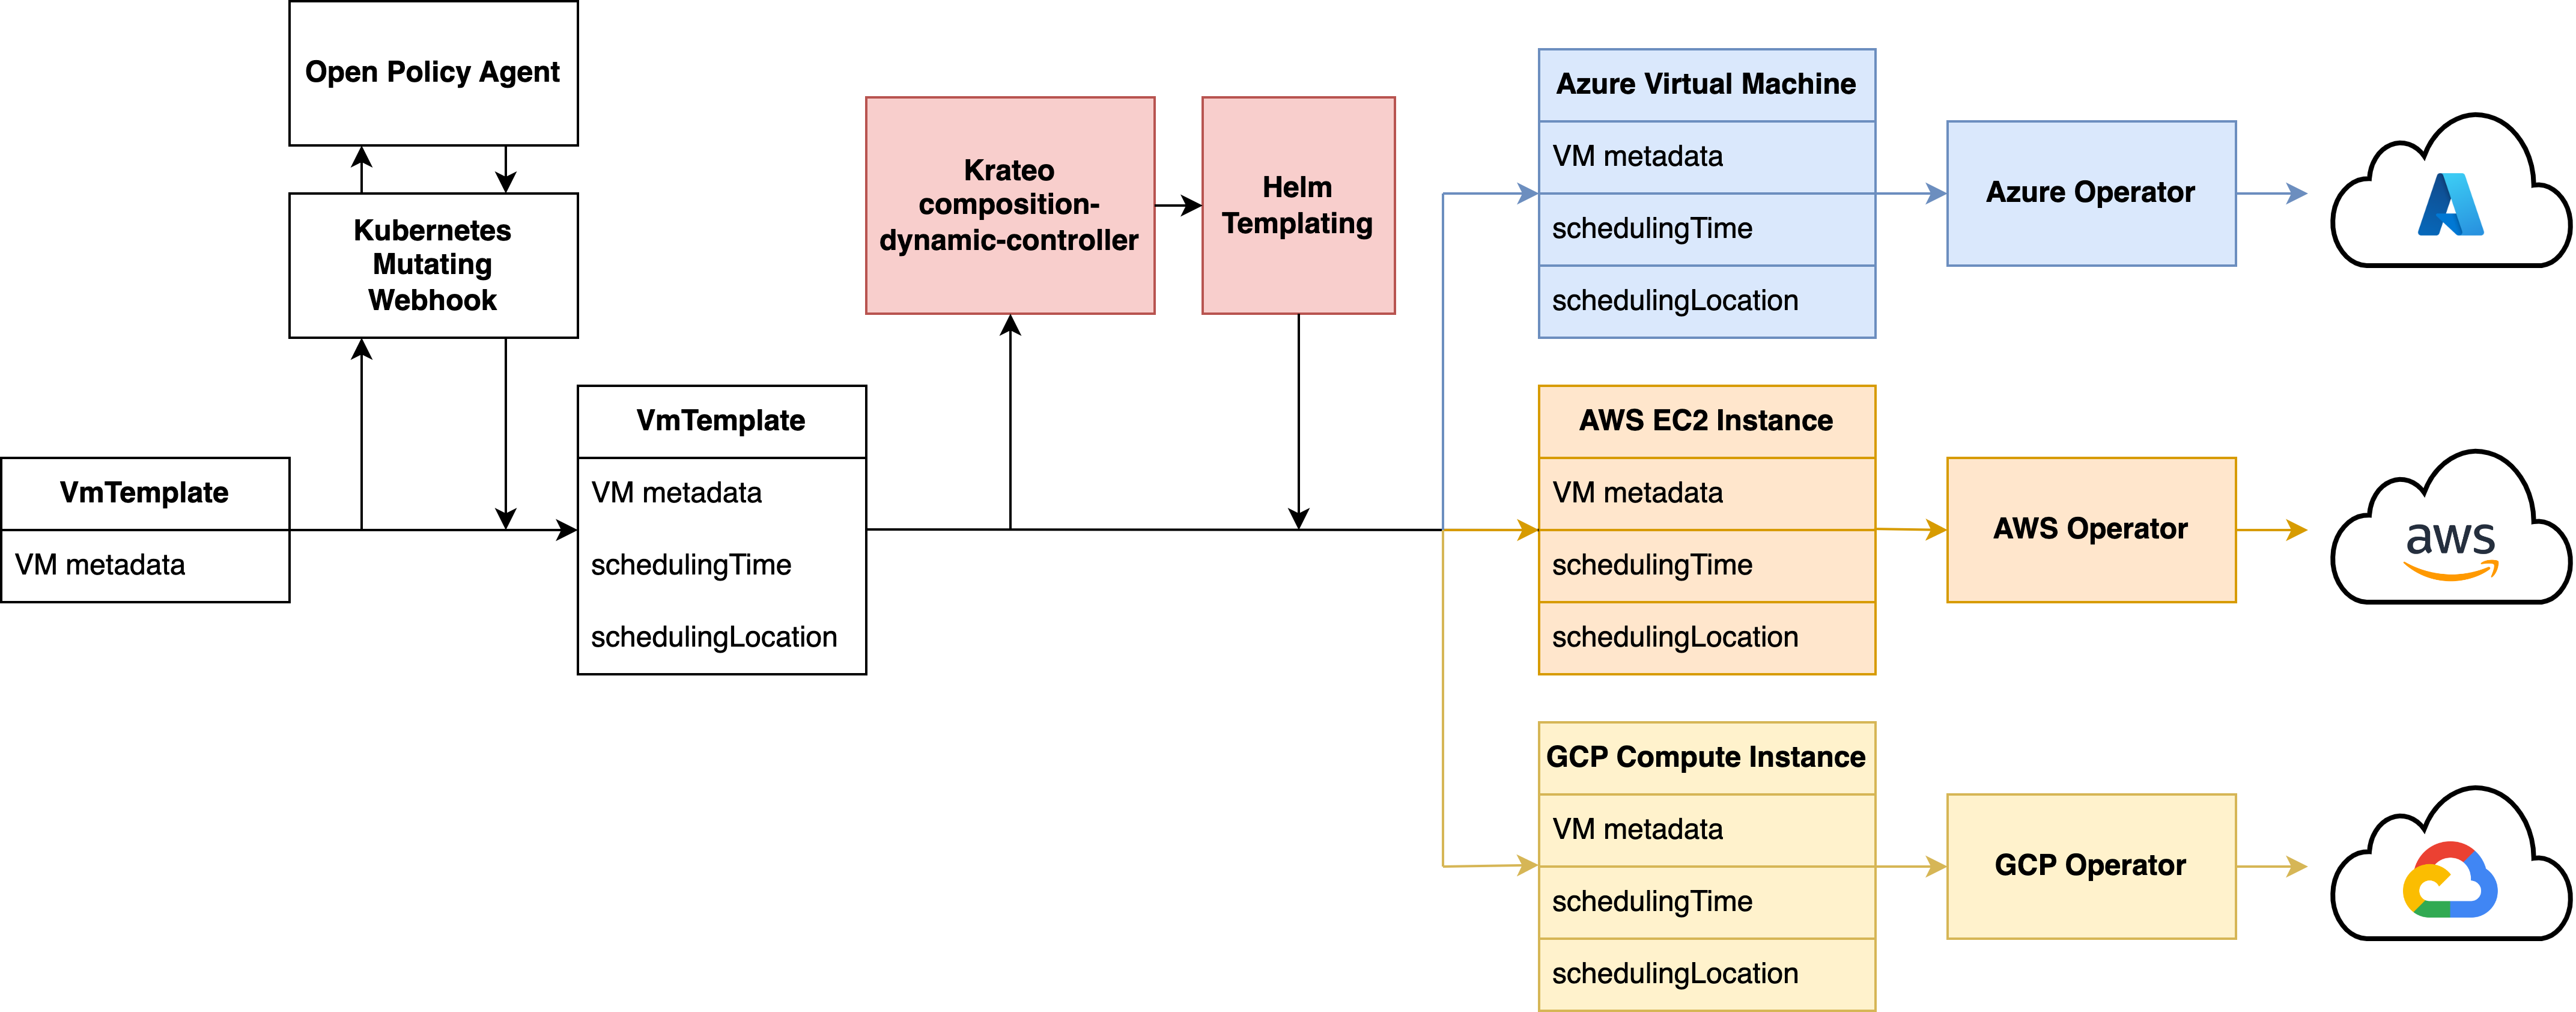
\includegraphics[width=1\linewidth]{images/krateo.png}
  \caption{Multi-cloud resource management with Krateo PlatformOps approach}
  \label{fig:krateo}
\end{figure}

what is krateo
developer platform
already described in section \ref{xyz}

Self-service platform for multi-cloud native resources

(generic VM mapped thanks to Krateo components, what is the added value)

generic workload resource definition
how to define it


Helm template engine (how to map to cloud provider specific resources, why is better)


Multi-cloud VMs list and mapping
We need to know which VMs (instance types) are actually available on Azure, AWS, GCP.
What to actually use to fetch the list and where to store it
How frequent the elements changes and how to update the list (this is done with policy updates (updates to contextual data))
How to match generic workload to candidate VMs instance types (that adhere to the generic workload specs), what is the mapping logic.
For example:
Requested VM (generic): (2 vCPU, 16 GiB)
Chosen VM instance: Azure Standard E2as v4
What are the steps of the process to identify the correct VM instance?

Use Cloud Providers API / CLI and store the records in a local DB. Regular scheduled updates.
For our PoC we could maybe use a small subset of all the available instance types.

Current approach:
Map (CPU, RAM) => InstanceType

This mapping is done through Helm templating when creating 

compostion definition


krateo cdc
The composition-dynamic-controller is an operator that is instantiated by the core-provider to manage the Custom Resources whose Custom Resource Definition is generated by the core-provider.

\section{Kubernetes Mutating Webhook Configuration}

[from k8s docs]

K8s mutating webhook is used to modify K8s custom resources with the data from policies. 
The K8s mutating webhook intercepts the CREATE or UPDATE API request, asks about policies (with also scheduling decision) and mutates the resource.

we can distinguish between two types of webhooks: validating and mutating.

we can distinguish two entities semantically different: the webhook configuration and the actual webhook service which perform mutation or validation

it could be a server that you need to implement to perform your own custum mutation or validation logic
it could be a service ready to use out of the box like OPA server

\begin{figure}[htb]
  \centering
  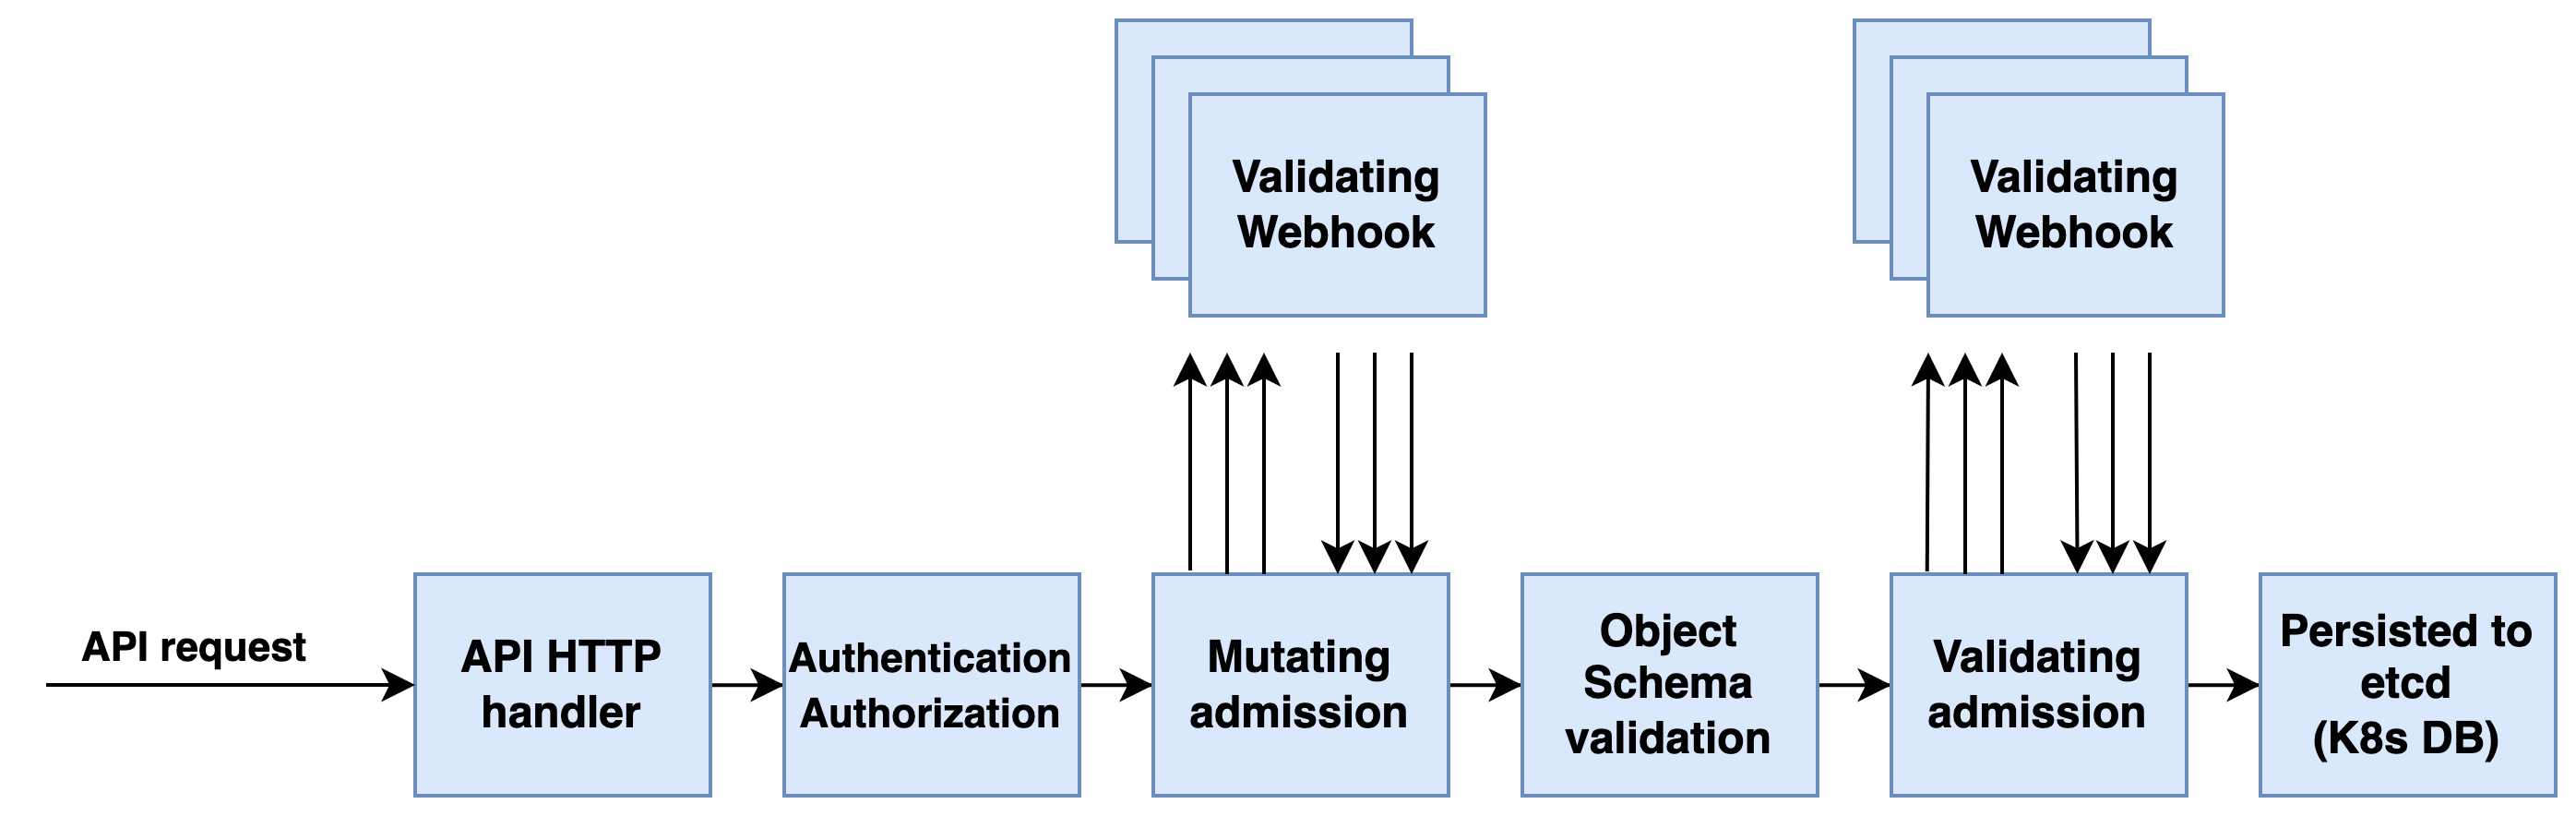
\includegraphics[width=1\linewidth]{images/k8s_admission.png}
  \caption{Kubernetes Admission Control}
  \label{fig:k8s_admission_control}
\end{figure}


service can be either a deployment with the related service
inside the cluster like seen in the image \ref{fig:k8s_webhook_example}

\begin{figure}[htb]
  \centering
  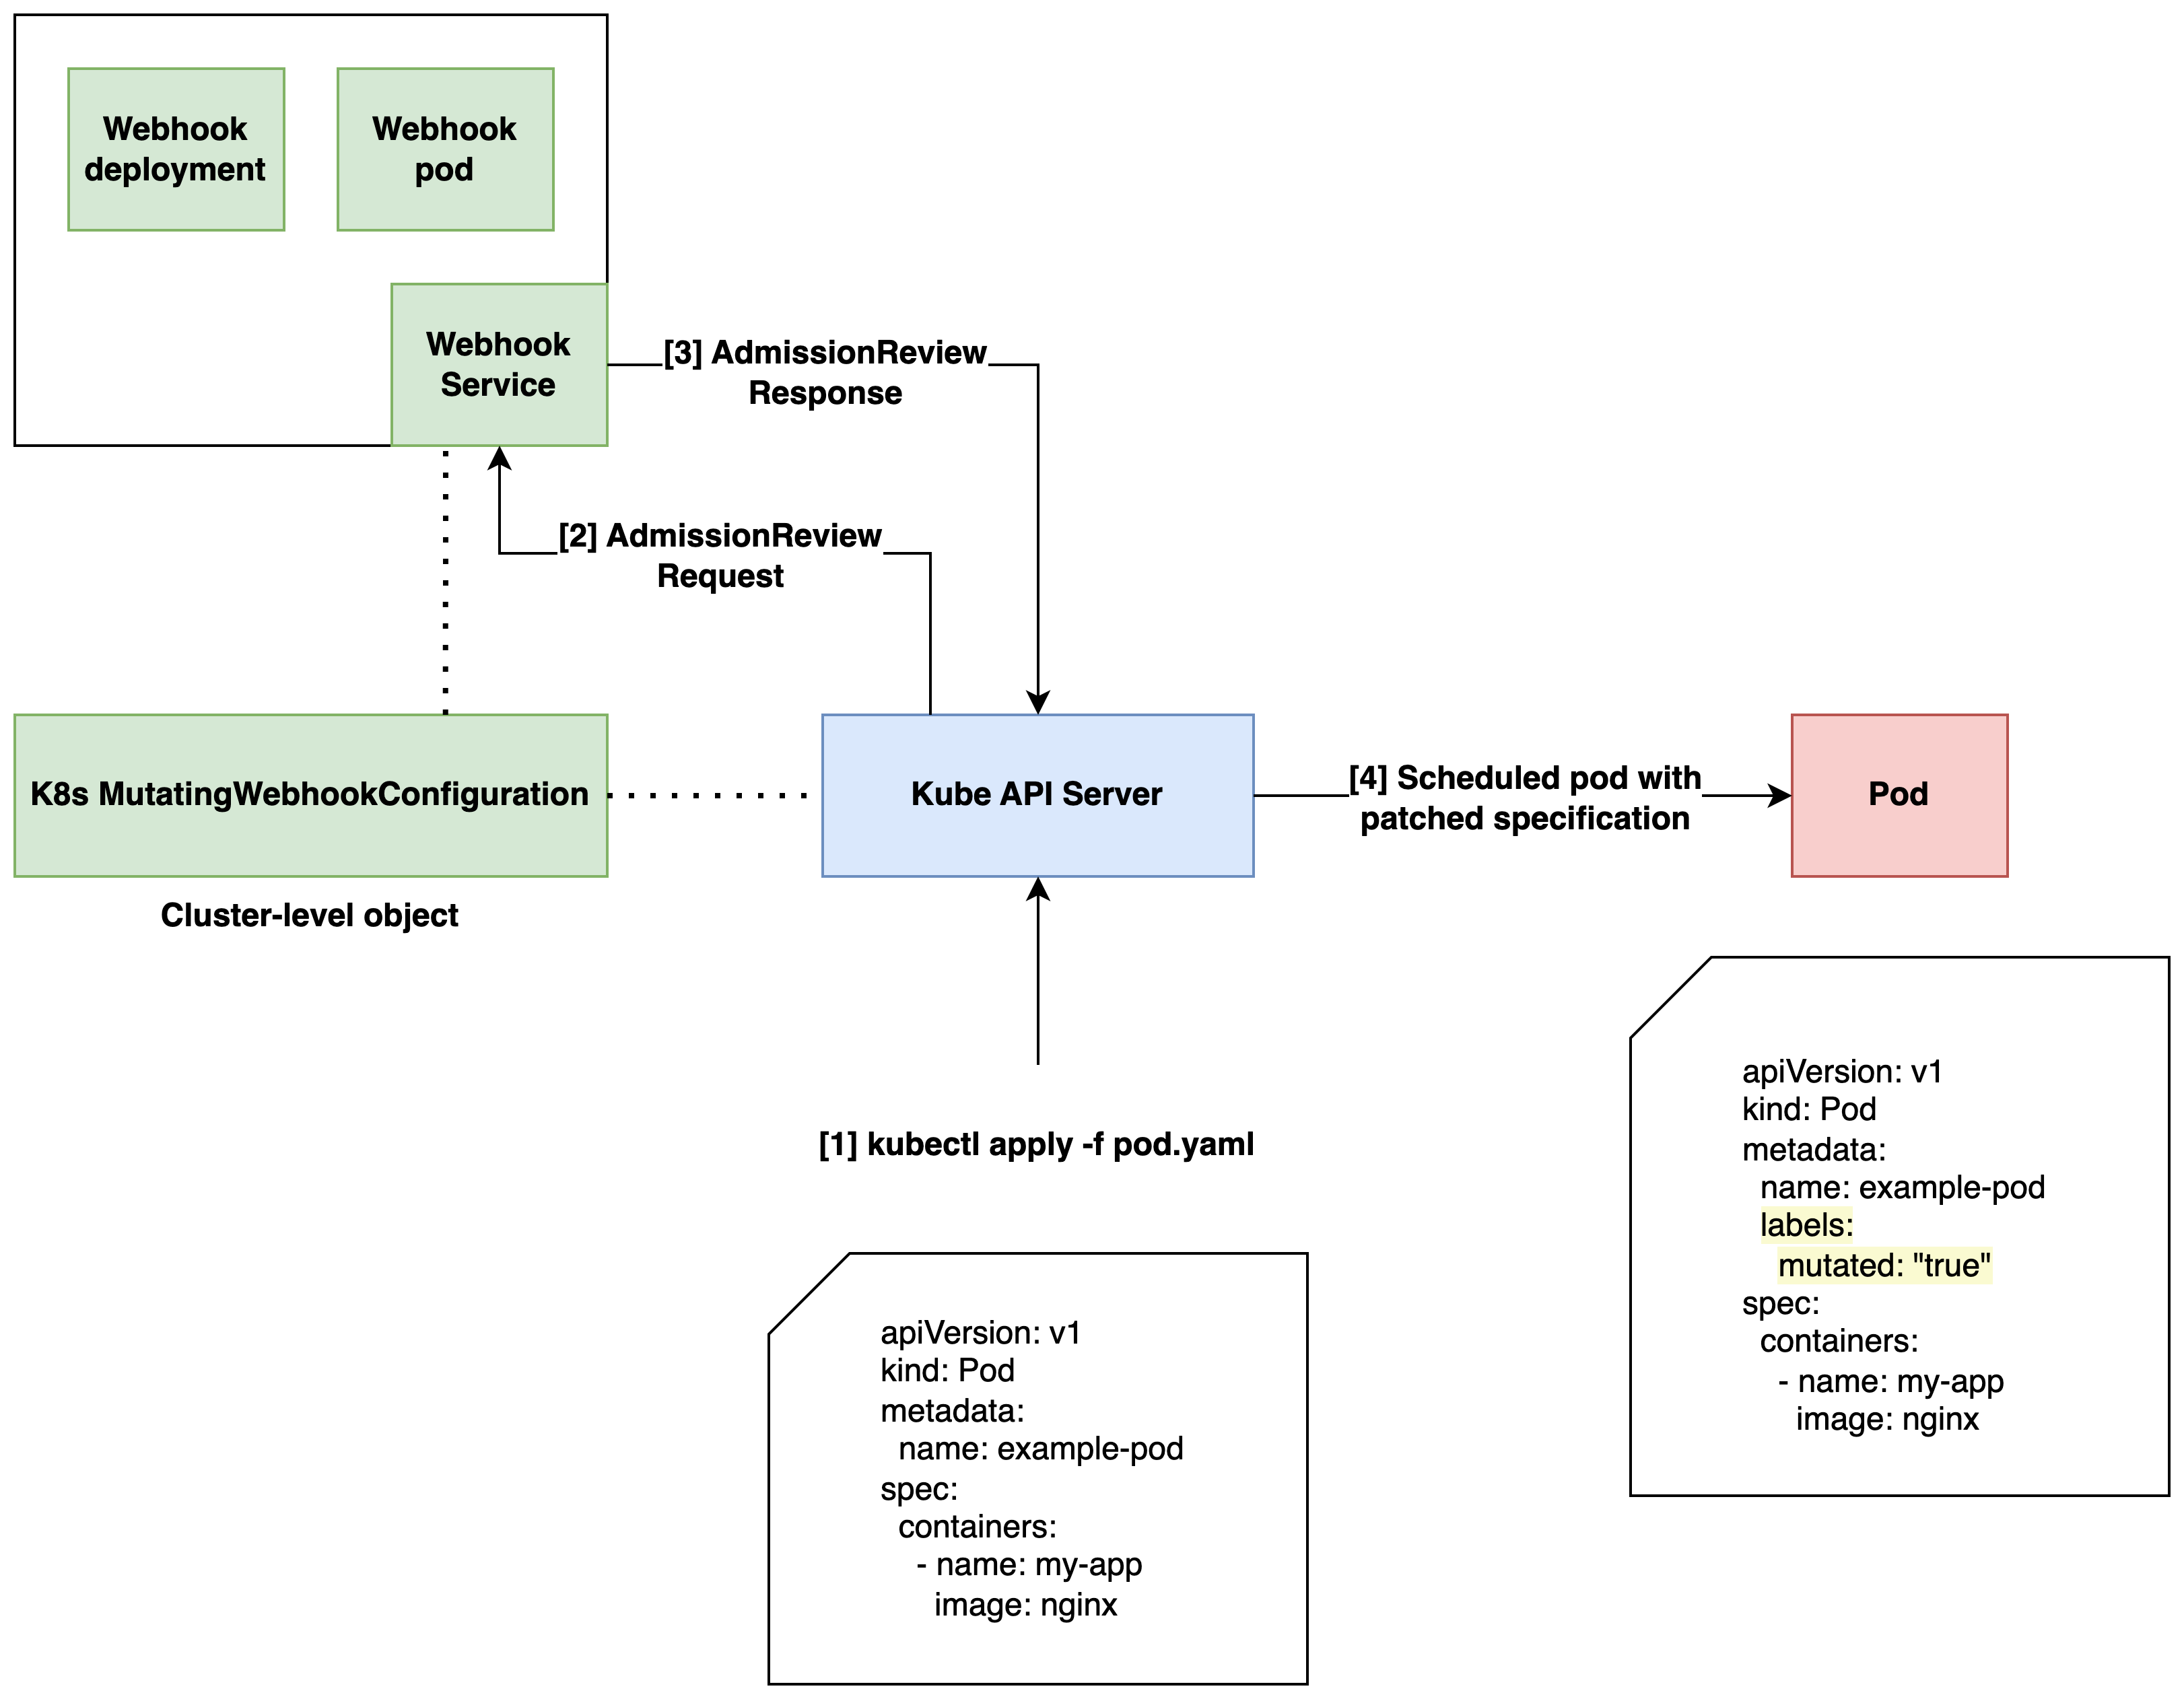
\includegraphics[width=1\linewidth]{images/k8s_webhook_example.png}
  \caption{Kubernetes Mutating Webhook example}
  \label{fig:k8s_webhook_example}
\end{figure}

[cite https://www.youtube.com/watch?app=desktop&v=Eb9pMSCTDjI for the image of the example]

\section{Multi-Cloud Integration through Kubernetes Operators}

The integration of operators from different cloud providers has enabled the development of an effective \textbf{multi-cloud system}, allowing seamless orchestration and provisioning of cloud resources across various cloud platforms. Namely, the system leverages Kubernetes operators from \textbf{Microsoft Azure}, \textbf{Google Cloud Platform (GCP)}, and \textbf{Amazon Web Services (AWS)}.

\subsection{Role of Kubernetes Operators}

Kubernetes operators work on the principle of Continuous Reconciliation, ensuring, in this case, that the desired state of the system, as defined by users, aligns with the actual state of provisioned cloud resources. In particular, Operators act as controllers that monitor, adjust, and manage external cloud resources within a Kubernetes-native environment. Inside the K8s lie the representation of the cloud resources, which are managed by the operators.
Key characteristics of operators include:
\begin{itemize}[itemsep=0.2pt, topsep=1pt]
  \item[$\bullet$] Managing external cloud resources within a Kubernetes cluster, providing a \textbf{unified interface} for multi-cloud deployments.
  \item[$\bullet$] Maintaining a \textbf{real-time representation} of provisioned cloud resources within Kubernetes.
  \item[$\bullet$] Using Custom Resources (CRs) to define cloud-specific resources in a \textbf{declarative} manner.
\end{itemize}

\subsection{Strategic Shift: From Custom Operator to Krateo Core Provider}

In our approach, we opted to replace a custom Kubernetes operator (``Synchronization Operator''), originally designed to handle the \textbf{mapping} from generic to cloud-specific resources, with \textbf{Krateo Core Provider}. This decision was motivated by the need for greater flexibility and maintainability in defining multi-cloud infrastructure components. As a matter of fact, the custom operator was originally designed to handle only virtual machines (VMs) mappings and extensions to support additional cloud resources would have required significant code changes and maintenance overhead for each additional resource type added.

Therefore instead of embedding business logic directly within a custom Kubernetes operator, in the current system implementation, we leverage the capabilities of \textbf{Helm templating} to dynamically generate cloud-provider-specific resources. More precisely, another Krateo component, the \textbf{Krateo composition-dynamic-controller} is leveraging Helm templating under the hood to generate Kubernetes resources starting from helm templates.
This approach, further described in the following sections, offers several advantages:

Simplified resource management:  Helm enables a standardized way define resources without maintaining complex operator logic.
Greater extensibility:  By externalizing the logic from the operator, future modifications and integrations with additional cloud providers become easier.
Reduced maintenance overhead: Operators typically require constant updates and refinements, while Helm-based resource generation minimizes the need for frequent code changes.

It must be noted that different cloud provider adopts different design choices for their Kubernetes operators and more in general for their overall infrastructure management. Therefore, for the creation of logically similar resources, like a virtual machine, the structure and the field of the resources can be different. 
These resources typically include:
\begin{itemize}[itemsep=0.2pt, topsep=1pt]
  \item[$\bullet$] Compute resources (e.g., VM instances, virtual machine templates)
  \item[$\bullet$] Networking components (e.g., virtual networks, subnets, security groups)
  \item[$\bullet$] Storage allocations (e.g., persistent volumes, cloud disks)
  \item[$\bullet$] Access management (e.g., resource groups, roles, authentication credentials)
\end{itemize}


For the purpose of this work we defined baseline infrastructure for each cloud provider in order to have a common ground for the system to work. This baseline infrastructure is composed by the minimum set of resources needed for a VM provisioning.

each providers has its complexities and nuances

vendor lock-in.





\newpage

\subsection{Azure Kubernetes Operator}

Microsoft Azure provides a Kubernetes operator called \textbf{Azure Service Operator v2} (ASO).
Currently, ASO supports more than 150 different Azure resources.
minimum set of resources needed for vm provisioning on Azure throgh Azure service operator is is:

\begin{itemize}[itemsep=0.2pt, topsep=1pt] \item[$\bullet$] Virtual Network 
\item[$\bullet$] Virtual Network Subnet
\item[$\bullet$] Network Interface
\item[$\bullet$] Virtual Machine
\end{itemize}

\begin{figure}[H]
\centering
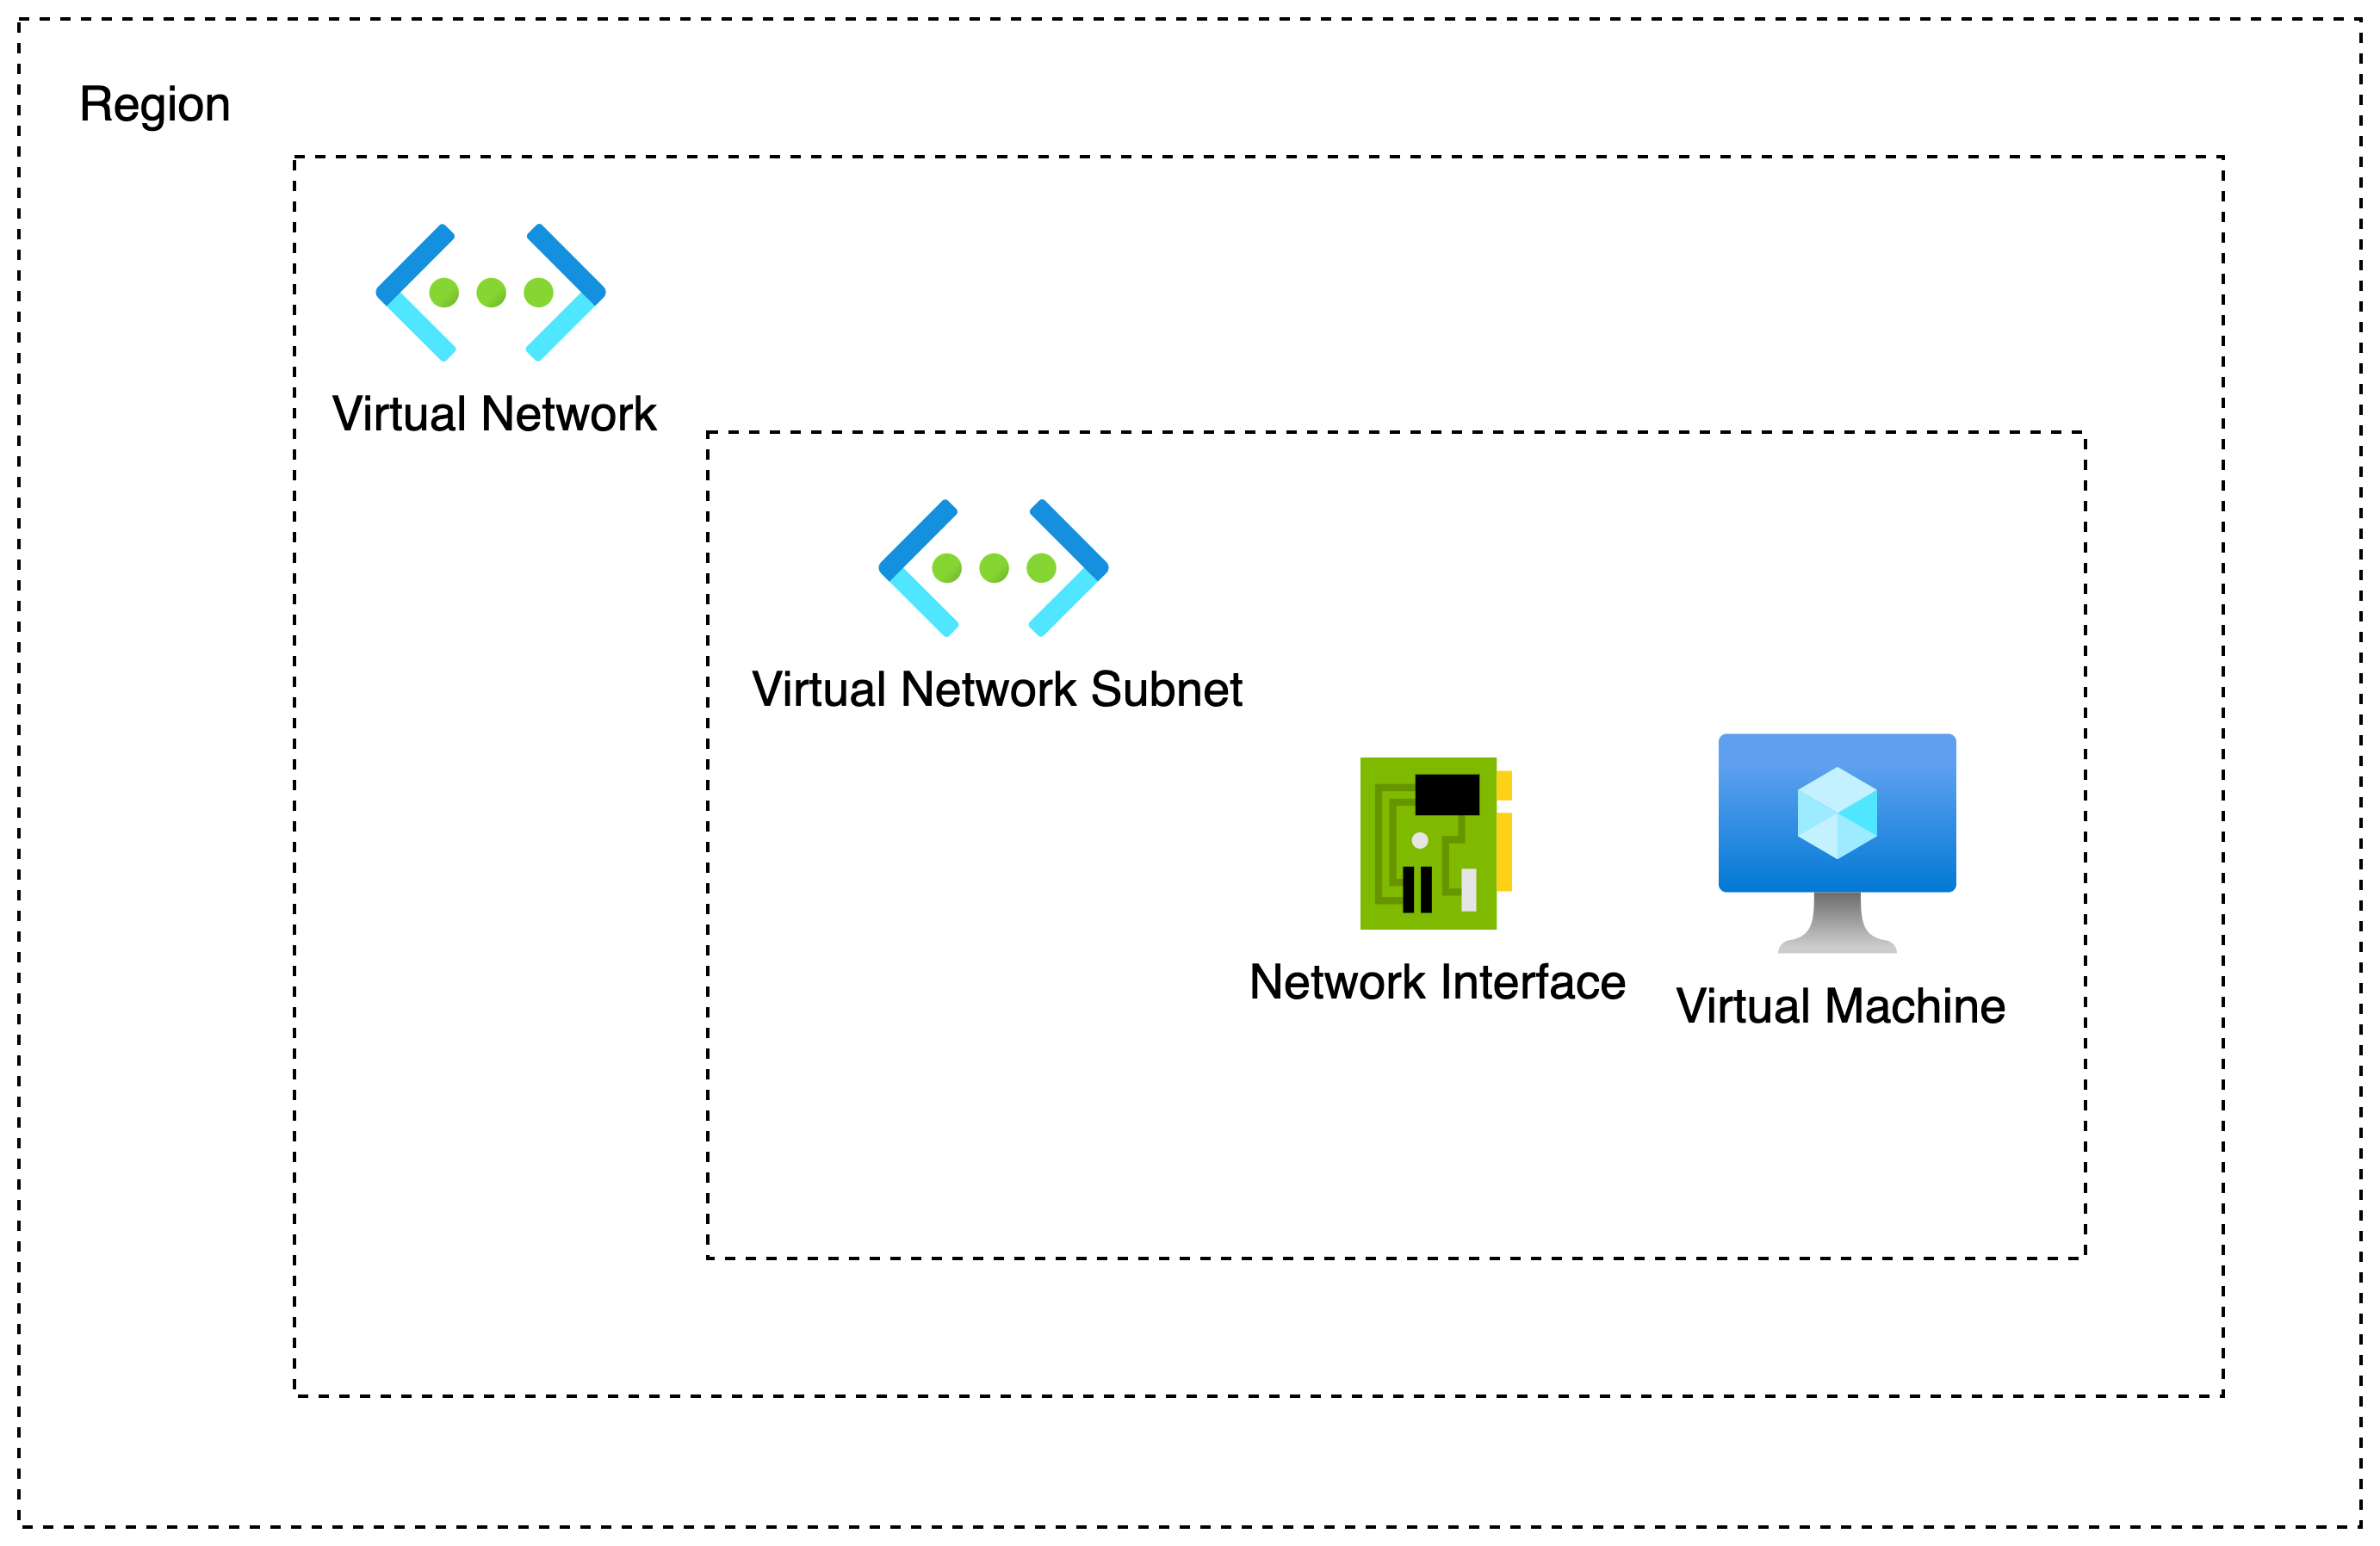
\includegraphics[width=0.75\linewidth]{images/azure.png}
\caption{Minimum set of Azure resources for VM provisioning}
\label{fig:azure}
\end{figure}






INSTANCE CR example











\subsection{GCP Operator}

minimum set of resources needed for vm deployment


\begin{figure}[H]
\centering
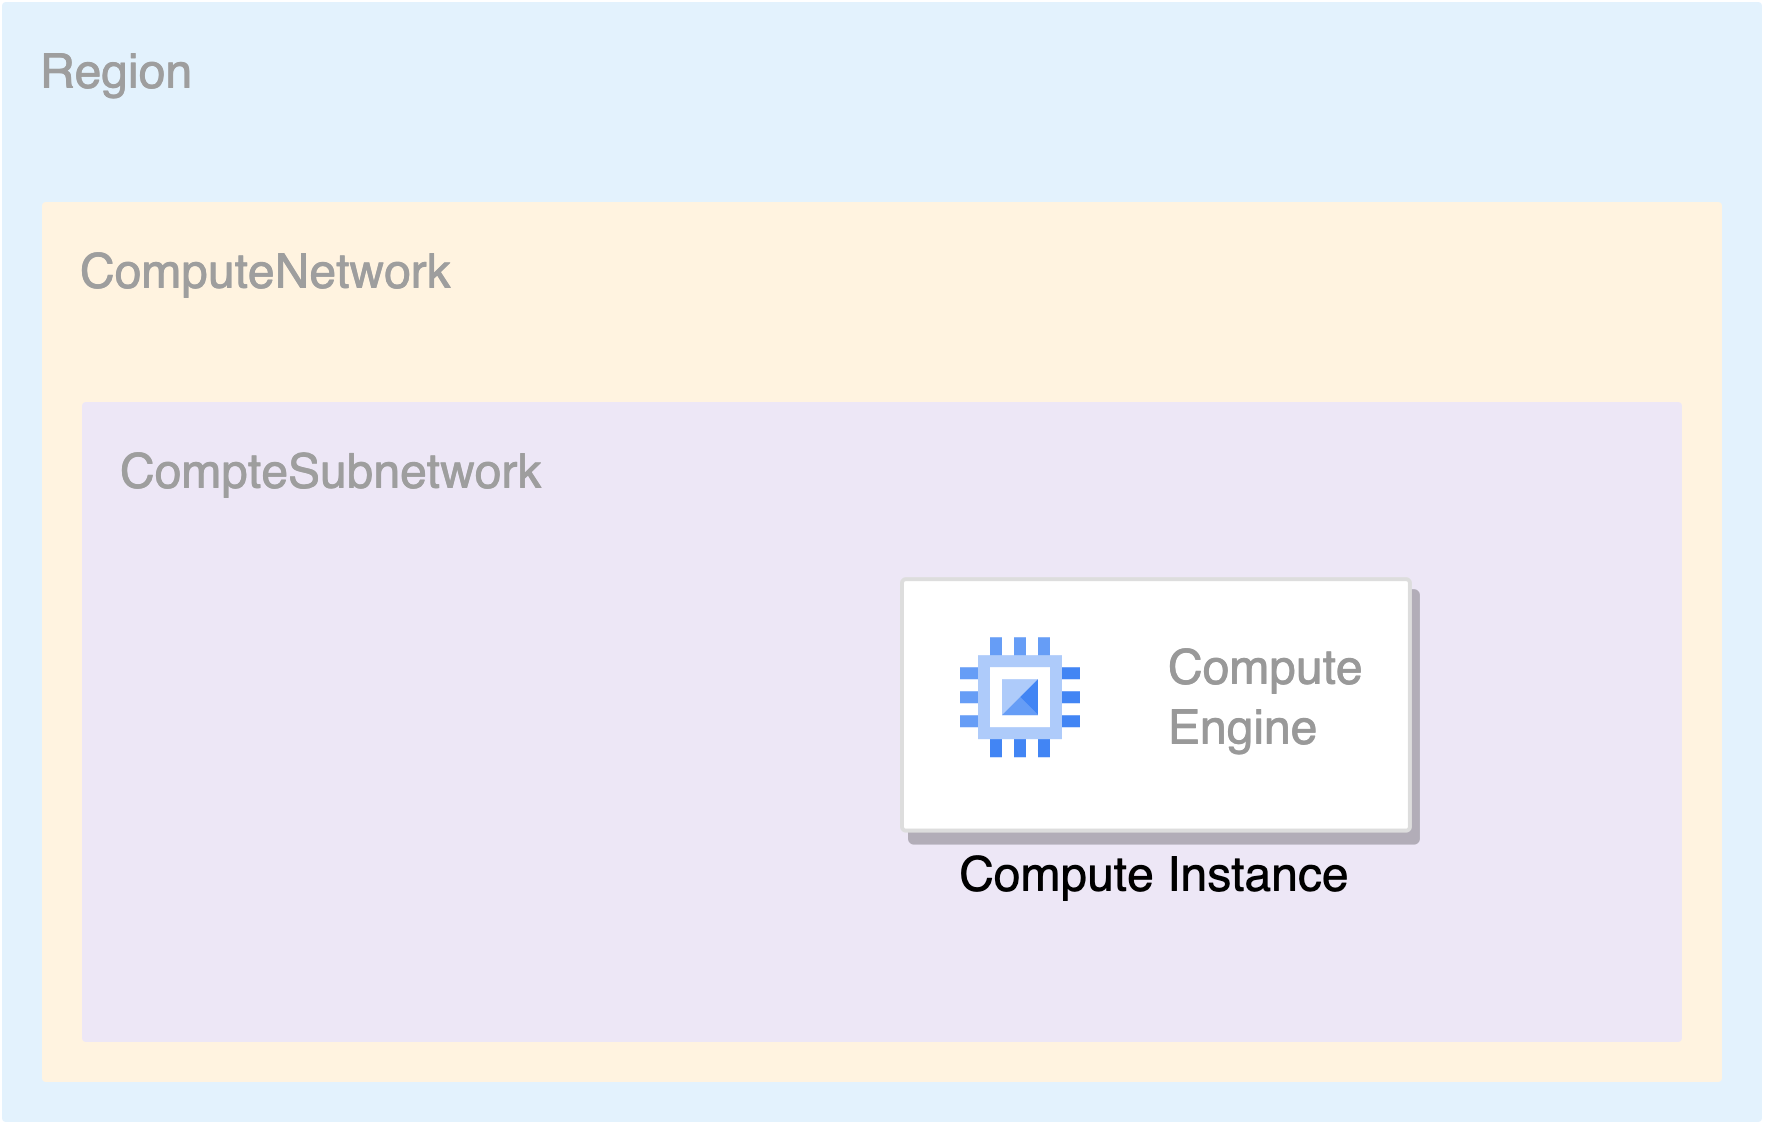
\includegraphics[width=0.75\linewidth]{images/gcp.png}
\caption{Minimum set of GCP resources for VM provisioning}
\label{fig:gcp}
\end{figure}




INSTANCE CR example

some fields are based on regions
some fields are based on zones


networkinterface is directly defined in the instance manifest,
no additional resource needed



\subsection{AWS Operator}

this is a collection of operators that are part of the AWS controllers for Kubernetes (ACK) project.

minimum set of resources needed for vm provisioning

\begin{itemize}[itemsep=0.2pt, topsep=1pt] 
\item[$\bullet$] VPC
\item[$\bullet$] Subnet
\item[$\bullet$] EC2 Instance
\end{itemize}






\begin{figure}[H]
\centering
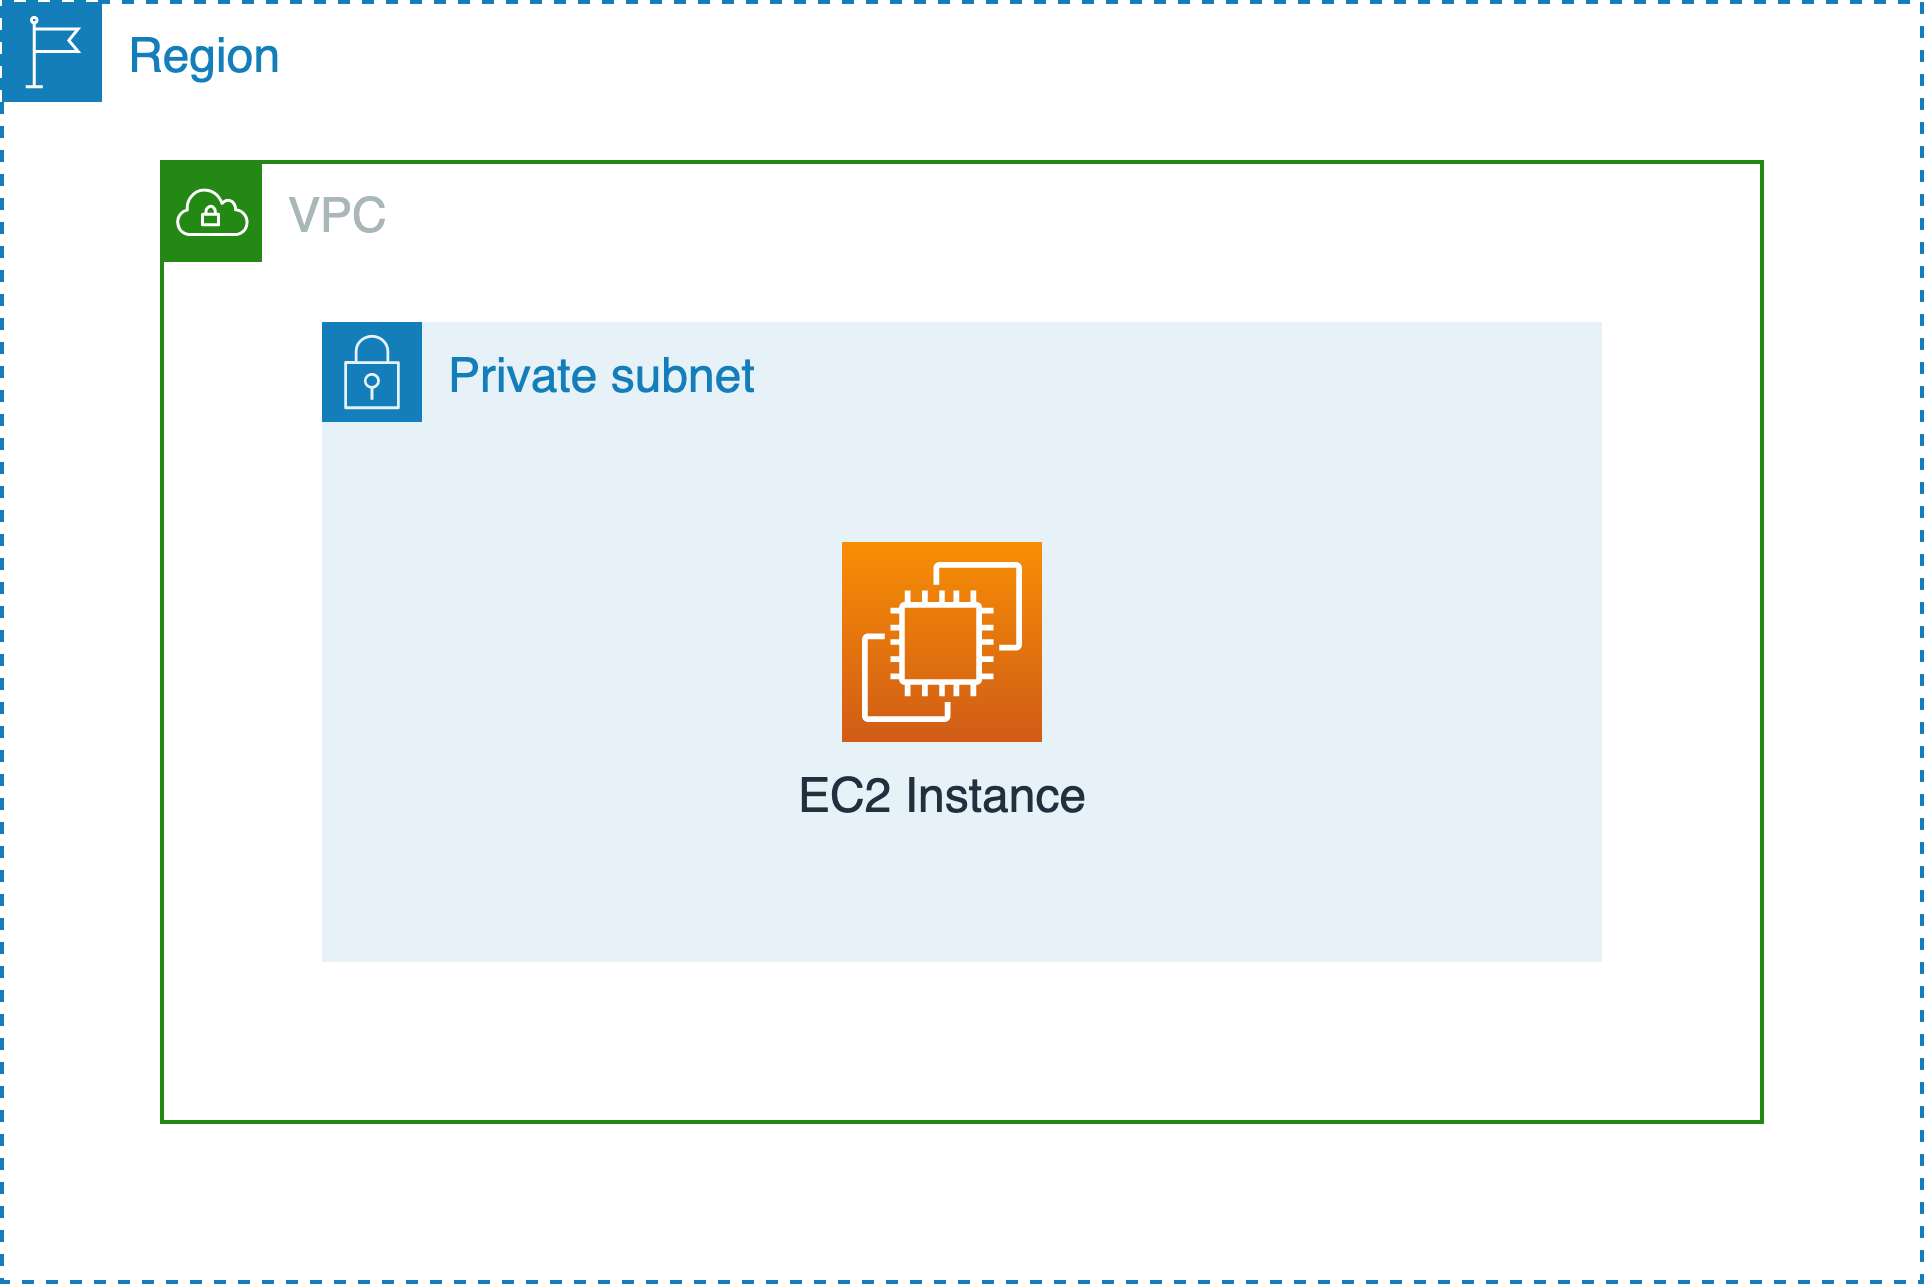
\includegraphics[width=0.75\linewidth]{images/aws.png}
\caption{Minimum set of AWS resources for VM provisioning}
\label{fig:aws}
\end{figure}


As described at the beginning of this section, the implementation approach adopted in our system ensures compatibility with diverse cloud provider design choices. Cloud providers may impose different constraints and best practices when managing Kubernetes-native resources, and the system is designed to adapt to these variations seamlessly.

One notable design choice observed with the AWS operator is the restriction on referencing some Kubernetes objects inside a Custom Resource (CR) manifest. This limitation means that developers cannot directly link a resource (e.g., a Virtual Machine) to another Kubernetes object (e.g., a Subnet) using built-in object references.

To overcome this limitation, our system leverages Helm’s lookup function, which dynamically retrieves Kubernetes object details at runtime. This method allows us to fetch required parameters without directly referencing Kubernetes objects in the CR, ensuring compatibility with the AWS operator’s design constraints. The following example demonstrates how the lookup function can be used to resolve subnet IDs dynamically and inject them into the CR manifest. \\

\begin{lstlisting}[language=yaml, caption={Helm Lookup example: dynamically resolving SubnetIDs}, label={lst:helm_lookup}]
...
apiVersion: ec2.services.k8s.aws/v1alpha1
kind: Instance
metadata:
  name: {{ .Values.vmName }}
  namespace: {{ .Values.namespace | default "greenops" }}
...
spec:
  ...
  subnetID: {{ (lookup "ec2.services.k8s.aws/v1alpha1" "Subnet" (.Values.namespace | default "greenops") (printf "%s-subnet" .Values.vmName)).status.subnetID }}
...
\end{lstlisting}

The Helm lookup function can be used to look up resources in a running cluster and its synopsis is: ``lookup apiVersion, kind, namespace, name -> resource or resource list'' \cite{helm_lookup}.
In the listing \ref{lst:helm_lookup}, the Helm lookup function retrieves the subnetID from a Subnet Custom Resource dynamically, based on the VM name and namespace. Then, the subnetID is injected into the Instance Custom Resource manifest, ensuring that the VM is provisioned in the correct subnet.

An example by the same AWS Operator where instead a direct reference to a resource is allowed is the one illustrated in listing \ref{lst:aws_direct_reference}. \\

\begin{lstlisting}[language=yaml, caption={AWS Operator direct reference example}, label={lst:aws_direct_reference}]
...
apiVersion: ec2.services.k8s.aws/v1alpha1
kind: Subnet
metadata:
  name: {{ .Values.vmName }}-subnet
...
spec:
  vpcRef: 
    from: 
      name: {{ .Values.vmName }}-vpc
      namespace: {{ .Values.namespace | default "greenops" }}
...
\end{lstlisting}

In this case, the Subnet Custom Resource manifest directly references the VPC Custom Resource using name and namespace since the Operator is designed to support this type of relationship. As explained before, this is determined by Operator design choices.


\subsubsection{Provider specific configurations}

An Amazon Machine Image (AMI) is a pre-configured image that provides the necessary software environment to set up and boot an Amazon EC2 instance \cite{aws_AMIs}. In other words, AMIs serve as a blueprint for launching virtual machines (VMs) in AWS.

When launching an instance, specifying an AMI is \textbf{mandatory}. The AMI must be compatible with the chosen EC2 instance type, ensuring that the selected image supports the required hardware and software configurations.

The following attributes define an AMI:
\begin{itemize}[itemsep=0.2pt, topsep=1pt] 
  \item[$\bullet$] Region: AMIs are region-specific
  \item[$\bullet$] Operating System: Determines the base OS (e.g., Ubuntu, Windows, RHEL) installed on the AMI.
  \item[$\bullet$] Processor Architecture: e.g., x86, ARM
  \item[$\bullet$] Root Device Type: Specifies whether the AMI uses an EBS-backed volume (Elastic Block Store) or Instance Store for storage.
  \item[$\bullet$] Virtualization Type: Defines whether the AMI supports paravirtual (PV) or hardware virtual machine (HVM) instances.
\end{itemize}


For the purpose of this research, only \textbf{Ubuntu-based AMIs} have been considered for provisioning virtual machines. Official Ubuntu AMIs were collected from a dedicated Ubuntu repository.
In order to select the most suitable AMI for a given VM, the system leverages Helm template engine to dynamically select the appropriate AMI ID based on the region and other parameters specified in the VmTemplate Kubernetes Custom Resource (CR).



\newpage

\section{Open Policy Agent (OPA)}

Open Policy Agent (OPA) is an open-source general-purpose \textbf{policy engine} that enables unified policy enforcement across cloud-native environments. OPA provides a declarative language called Rego enabling a paradigm known as ``\textbf{Policy as Code}" \cite{opa_docs}.

Open Policy Agent can be integrated as a sidecar container, host-level daemon, or library to perform policy decisions for a plethora of use cases: microservices, Kubernetes admission control, CI/CD pipelines, API gateways and more \cite{opa_docs}. 

In the context of our system, OPA and the Policy-as-Code paradigm are used to enforce policies for workload scheduling: encoding the output of a scheduling decision coming from an external GreenOps Scheduler and ensuring compliance with additional policies related to latency requirements and legal constraints.

\subsection{Policy as Code paradigm}

According to AWS, Policy-as-Code (PaC) is a software automation approach which is similar to Infrastructure-as-Code (IaC) \cite{pac_aws}. PaC helps assess company system configurations and validate compliance requirements through software automation \cite{pac_aws}. The perceived value of this type of automation in the software development lifecycle has grown significantly in modern enterprises. This large adoption is probably driven by the inherent consistency and reliability it provides, ensuring standardized enforcement of policies and reducing human error \cite{pac_aws}.

OPA's generic defintion of policy is: ``\textit{A policy is a set of rules that governs the behavior of a software service}" \cite{opa_philosophy}. OPA provides a high-level declarative language called \textbf{Rego} to define policies in a flexible manner. One of OPA's key strengths is its \textbf{domain-agnostic design}, allowing it to enforce policies across various systems and environments. This makes it highly adaptable to different use cases, ranging from access control to infrastructure security. Some representative examples of policies that OPA can enforce include:

\begin{itemize}[itemsep=0.2pt, topsep=1pt] \item[$\bullet$] Restricting which image registries can be used for deploying new Pods in a Kubernetes cluster.
\item[$\bullet$] Controlling whether a specific user is permitted to perform delete operations on certain resources.
\item[$\bullet$] Enforcing network security policies, such as blocking external access to sensitive services.
\item[$\bullet$] Ensuring infrastructure compliance, for example, by verifying that new cloud resources to be provisioned follow predefined security configurations.
\item[$\bullet$] Enforcing that new deployed servers must have the prefix ``server-" in their name.
\end{itemize}

Therefore, the use cases covered span from role-based access control to container image security and beyond.
\newline


Another important aspect of OPA is that it effectively \textbf{decouples} policy decision-making from policy enforcement, enabling organizations to implement consistent and scalable authorization across their systems \cite{test}.
In practice, this means that when a software module needs to make a policy decision, it queries OPA, supplying relevant data as input. In other words, policy decisions are \textbf{offloaded} to OPA rather than being hardcoded within individual services. This approach offers several key advantages:
\begin{itemize}[itemsep=0.2pt, topsep=1pt]
  \item[$\bullet$] \textbf{Centralized policy management}: policies are defined in a single location, ensuring uniform enforcement across all services.
  \item[$\bullet$] \textbf{Improved maintainability}: updating policies does not require modifying, recompiling or redeploying application code, reducing complexity and deployment overhead.
  \item[$\bullet$] \textbf{Greater flexibility}: policies can be dynamically updated (e.g., with CI/CD approaches) based on evolving security and compliance requirements 
  \item[$\bullet$] \textbf{Scalability}: since OPA and application modules are not tightly coupled.
\end{itemize} 

\subsection{OPA architecture overview}

As mentioned in the introduction to this section, one common approach to integrating OPA into a software system is by deploying it as a host-level daemon. The latter is essentially a lightweight server that processes policy queries via HTTP requests. This setup allows services to offload policy decision-making to OPA in a scalable and efficient manner since the two entities are not tightly coupled.

A standard OPA deployment consists of three main components:

\begin{itemize}[itemsep=0.2pt, topsep=1pt]
\item[$\bullet$] \textbf{OPA Server} – The core service that evaluates policy queries and returns decisions based on defined rules, contextual data and input data.
\item[$\bullet$] \textbf{OPA Policies} – Rules written in the Rego language that define the logic to be enforced.
\item[$\bullet$] \textbf{Data} – Optional contextual information, typically structured in JSON format, that policies use to make informed decisions along with input data.
\end{itemize}

To facilitate deployment and management, Rego policies and associated contextual data are packaged into \textbf{policy bundles}, as described in section \ref{sec:opa_policies}. These bundles enable version-controlled, centralized policy distribution, ensuring consistency and maintainability across distributed environments. \newline


\begin{figure}[htb]
\centering
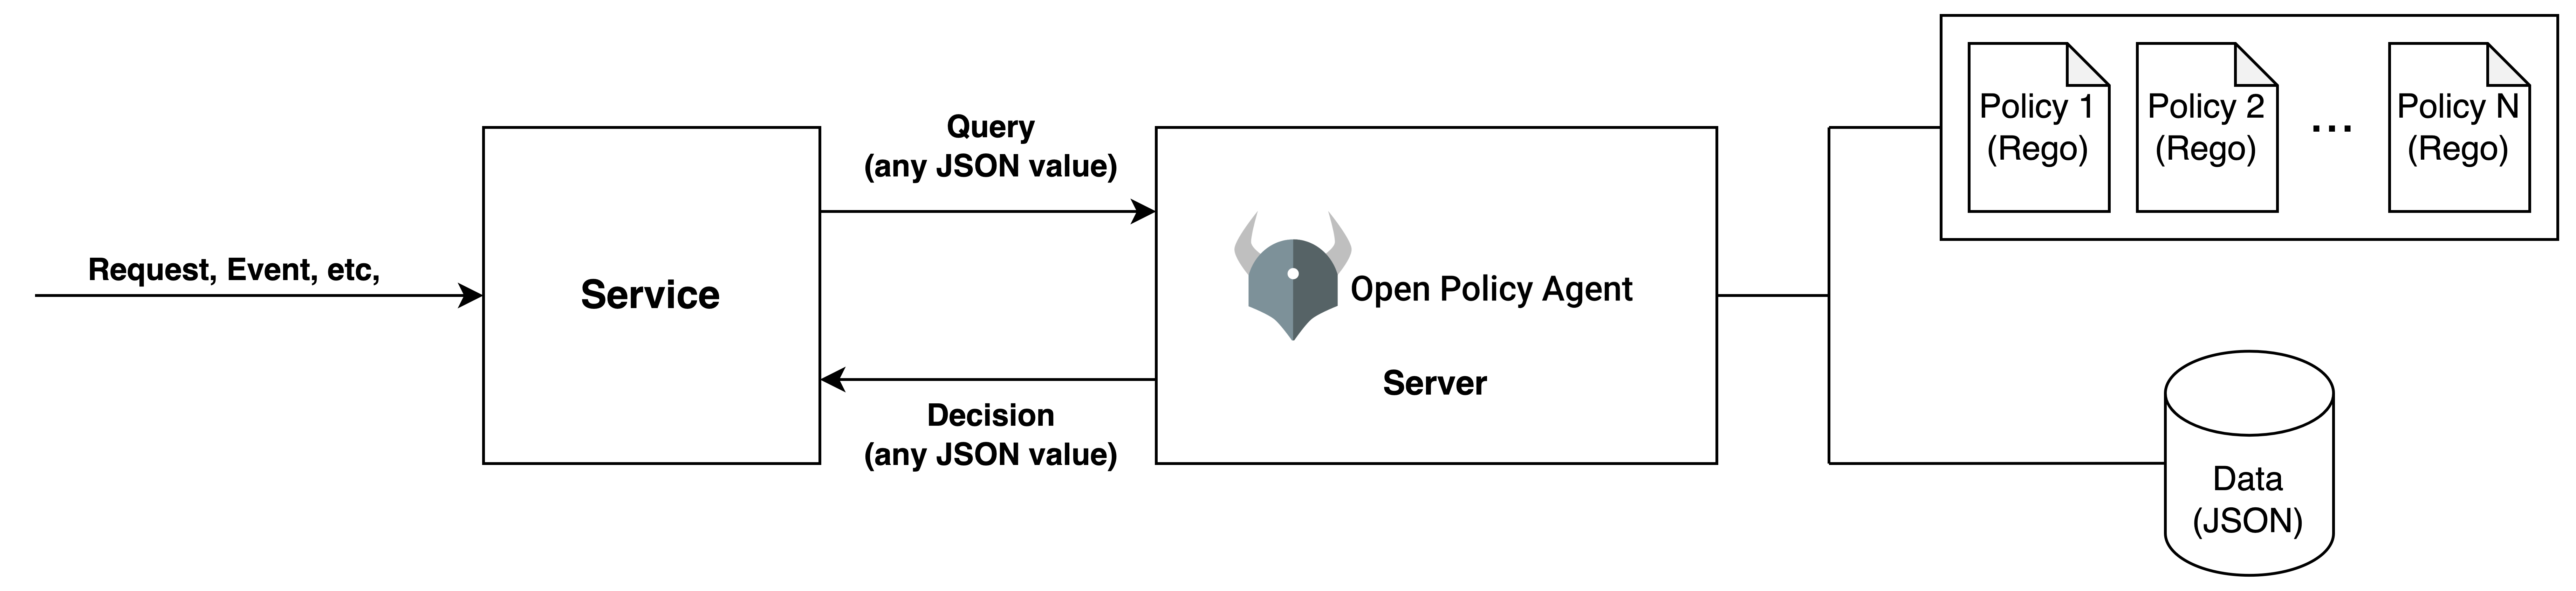
\includegraphics[width=1\linewidth]{images/OPA.png}
\caption{OPA architecture}
\label{fig:opa_architecture}
\end{figure}


OPA accepts arbitrary structured data as input.
and  Like query inputs, your policies can generate arbitrary structured data as output.

\subsection{OPA and external data}

types of external data strategies

http.send()
paramters 

\subsection{OPA integration with Kubernetes}

In Kubernetes admission control, policy enforcement is handled by the \textbf{Kubernetes API server} itself. OPA makes the policy decisions when queried by the admission controller, but the actual enforcement (namely allowing or denying requests) is executed by Kubernetes' built-in admission control mechanisms. This workflow is represented in figure \ref{fig:webhook_opa} where \textbf{AdmissionrReview request} and \textbf{AdmissionReview response} are respectively input and output of the whole OPA section. The API Server sends the entire Kubernetes object in the webhook request to OPA. %cite OPA kubernetes primer
The Kubernetes API server will use the received AdmissionReview response for its decision. \\
%\cite{opa_philosophy}

\begin{figure}[htb]
\centering
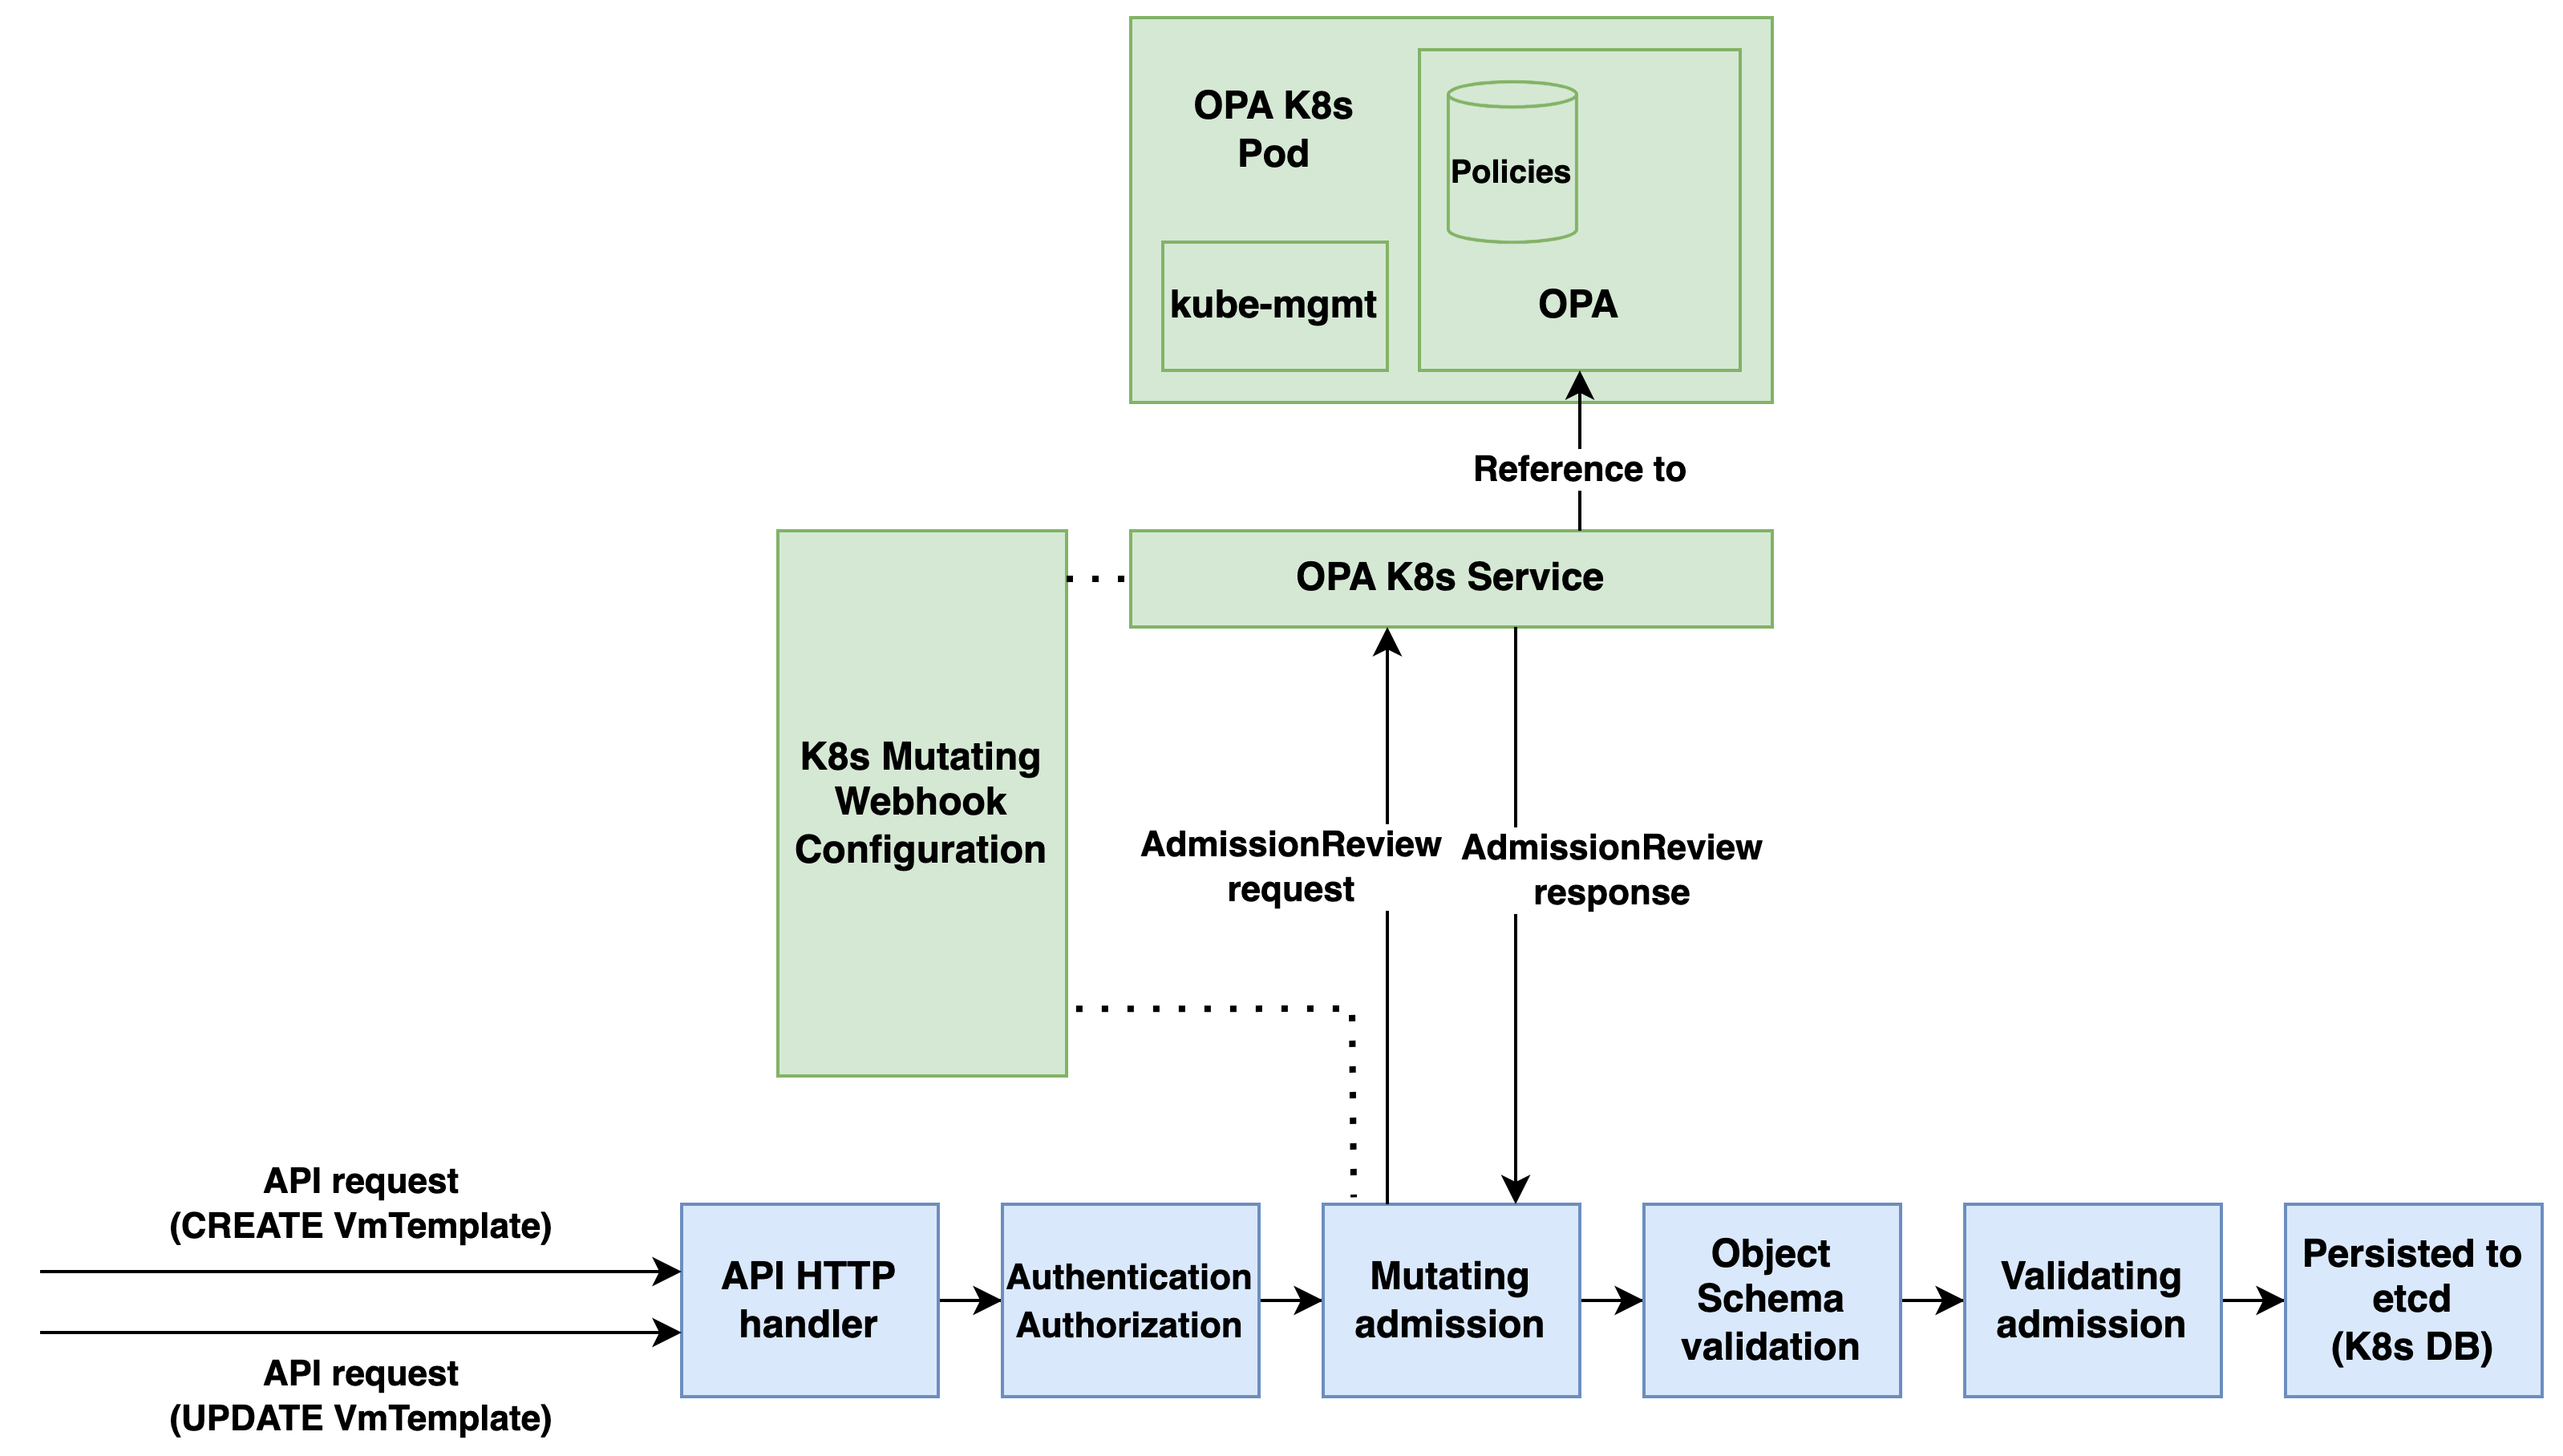
\includegraphics[width=1\linewidth]{images/webhook.png}
\caption{Kubernetes mutating webhook and OPA integration}
\label{fig:webhook_opa}
\end{figure}

In a Kubernetes deployment, an OPA Pod typically consists of the following containers:
\begin{itemize}[itemsep=0.2pt, topsep=1pt]
  \item[$\bullet$] OPA server container
  \item[$\bullet$] \textbf{kube-mgmt} container \\
\end{itemize} 

The kube-mgmt container functions as a \textbf{sidecar container} within a Kubernetes Pod. The sidecar container pattern is a common Kubernetes design paradigm in which auxiliary containers run alongside the main application container within the same Pod. These additional containers serve to enhance, extend, or support the primary application's functionality without modifying its core logic \cite{sidecar_containers}. 
The primary responsibility of kube-mgmt is to replicate Kubernetes resources into the OPA instance (OPA container). This operation is essential for OPA to access and evaluate policies based on real-time cluster state, enabling dynamic policy enforcement. By synchronizing these resources, kube-mgmt ensures that OPA has an up-to-date view of relevant Kubernetes objects.
This is especially useful to enforce policies that deals with naming conflicts, where OPA needs to check existing names in the cluster for the decision \cite{kube-mgmt}.
Additionally, it allows for loading policies directly from the Kubernetes cluster by retrieving them in the form of ConfigMaps. This feature is particularly useful when policies need to be dynamically updated based on the current state of the cluster \cite{kube-mgmt}. However, in the system described in this thesis, this latter feature is not employed in the current implementation as we are using policy bundles for policy distribution.

In the current system configuration, the kube-mgmt container is deployed to facilitate resource replication, ensuring that Kubernetes resources, namely VmTemplate resources, are synchronized with the OPA instance. However, at present, no policy requires interrogation of VmTemplate resources that are already present in the system.
Looking ahead, future policies could leverage VmTemplate resource information to enforce naming conflict resolution, quota management, or additional constraints.

\newpage

\subsection{OPA policies}
\label{sec:opa_policies}

%example of a policy:
%(https://www.openpolicyagent.org/docs/latest/kubernetes-primer/)





As OPA official documentation describes, when the Kubernetes AdmissionReview request from the webhook arrives, it is binded to the OPA input document and generates the default, ``root", decision: \textit{system.main}
%\cite

The root policy, in the case of Kubernetes admission control, is responsible for generating the AdmissionReview response in accordance with the Kubernetes API specifications. It is the duty of the policy developer to write Rego code that produces a well-formed AdmissionReview response, ensuring that the OPA server can then correctly communicate its decision to the Kubernetes admission controller.
%cite

It is deemed useful to show one of the simplest and common example of a OPA policy in the \textbf{Kubernetes admission control context}. That is: to ensure all images for Kubernetes Pods come from a trusted registry, namely \textit{unitn.it}. \\


It is important to note that, in this case, due to the simplicity of the policy, no additional contextual data in JSON format is required.


policy compilation
policy are compiled
compile time errors like merge errors if data is clashing for instance



\begin{comment}
    \lstset{
   language=Go,
   basicstyle=\ttfamily\small,
   breaklines=true,
   showstringspaces=false,
   commentstyle=\color{green!60!black},
   keywordstyle=\color{blue},
   stringstyle=\color{purple},
   numberstyle=\tiny,
   numbers=left,
   backgroundcolor=\color{gray!10},
   frame=single,
   captionpos=b
}
\end{comment}


\begin{lstlisting}[language=Rego, caption={Rego policy for Pods registry},
label=lst:rego_data_mapping]                              
deny contains msg if {                                                      
    input.request.kind.kind == "Pod"                                        
    image := input.request.object.spec.containers[_].image                  
    not startswith(image, "unitn.it/")                                     
    msg := sprintf("image '%v' comes from untrusted registry", [image])     
}
\end{lstlisting}

\begin{lstlisting}[language=Rego, caption={Rego ``root" policy (system.main)}]
package system

import data.kubernetes.admission

main := {
	"apiVersion": "admission.k8s.io/v1",
	"kind": "AdmissionReview",
	"response": response,
}

default uid := ""

uid := input.request.uid

response := {
	"allowed": false,
	"uid": uid,
	"status": {"message": reason},
} if {
	reason := concat(", ", admission.deny)
	reason != ""
}

else := {"allowed": true, "uid": uid}
\end{lstlisting}


\newpage
\lstset{style=jsonstyle}
\begin{lstlisting}[caption={AdmissionReview request}]
{
    "apiVersion": "admission.k8s.io/v1",
    "kind": "AdmissionReview",
    "request": {
        "kind": {
            "group": "",
            "kind": "Pod",
            "version": "v1"
        },
        "object": {
            "metadata": {
                "name": "myapp"
            },
            "spec": {
                "containers": [
                    {
                        "image": "bitnami/node:22",
                        "name": "nodejs"
                    }
                ]
            }
        }
    }
}
\end{lstlisting}

\lstset{style=jsonstyle}
\begin{lstlisting}[caption={AdmissionReview response}]
{
    "apiVersion": "admission.k8s.io/v1",
    "kind": "AdmissionReview",
    "response": {
        "allowed": false
        "status": {
            "message": "image 'bitnami/node:22' comes from untrusted registry"
        }
    }
}
\end{lstlisting}

Therefore, in this specific case, the creation of the Kubernetes Pod will be \textbf{denied}. OPA is responsible for \textbf{decision-making}, determining that the request do not complies with the defined policies, while the Kubernetes API server, using the AdmissionReview response generated by OPA, handles \textbf{policy enforcement}, effectively rejecting the CREATE request since it violates the specified rules.

\subsection{OPA Policy bundles}
\label{sec:opa_bundles}

An OPA policy bundle is a collection of policies and optional associated contextual data. More precisely, a bundle is a standardized way to package policies, facilitating version control and distribution \cite{opa_bundles}. As a matter of fact, a single policy bundle can be potentially used by multiple OPA instances.
A policy bundle mainly consists of:
\begin{itemize}[itemsep=0.2pt, topsep=1pt]
  \item[$\bullet$] \textbf{Rego policy files} defining the logic.
  \item[$\bullet$] \textbf{Data files} (in JSON or YAML format) containing contextual information required for policy evaluation (e.g., cloud region mappings).
\end{itemize} 

Policy bundles can be distributed through a variety of mechanisms such as remote HTTP servers (e.g., NGINX) and object storage services (e.g., Amazon S3, Google Cloud Storage, Azure Blob Storage) \cite{opa_bundles}.
One of the most convenient approaches is packaging them as \textbf{OCI (Open Container Initiative) images} \cite{oci} and this is the approach adopted in the system described in this thesis.

Once packaged as OCI images, policy bundles can be pulled by OPA servers from a container registry at predefined time intervals. This allows policy updates to be deployed in OPA \textbf{without requiring manual intervention} or \textbf{service restarts}, ensuring that enforcement mechanisms remain up to date with the latest compliance requirements identified and implemented by the organization. This is crucial for instance when dealing with \textbf{critical security policies} that need to be updated frequently, maybe in response to the discoveries of new CVEs. In the context of our system, such timely updates are not essential but the OPA is designed to be able to handle them if needed.
To ensure continuous policy enforcement while maintaining high operational efficiency, a CI/CD approach is adopted for policy management in the context of our system.
As a matter of fact, policies are maintained in a \textbf{version-controlled hosted repository} (i.e., on GitHub), where updates like tagging (``git tag'') trigger an automated pipeline (e.g., using GitHub Actions) responsible for building, packaging into a OCI image, and publishing the policy bundle to a container registry (e.g., Docker Hub).
One of the major advantages of this approach is the ability to dynamically update policies without requiring OPA pods to restart as there is an \textbf{hot-reload} of policies done at application level by OPA (``loaded on the fly'') \cite{opa_bundles}. This is particularly useful in production environments where service availability is critical and downtime must be minimized. 
The overall process of policy distribution is illustrated in figure \ref{fig:opa_bundles}.

\begin{figure}[H]
\centering
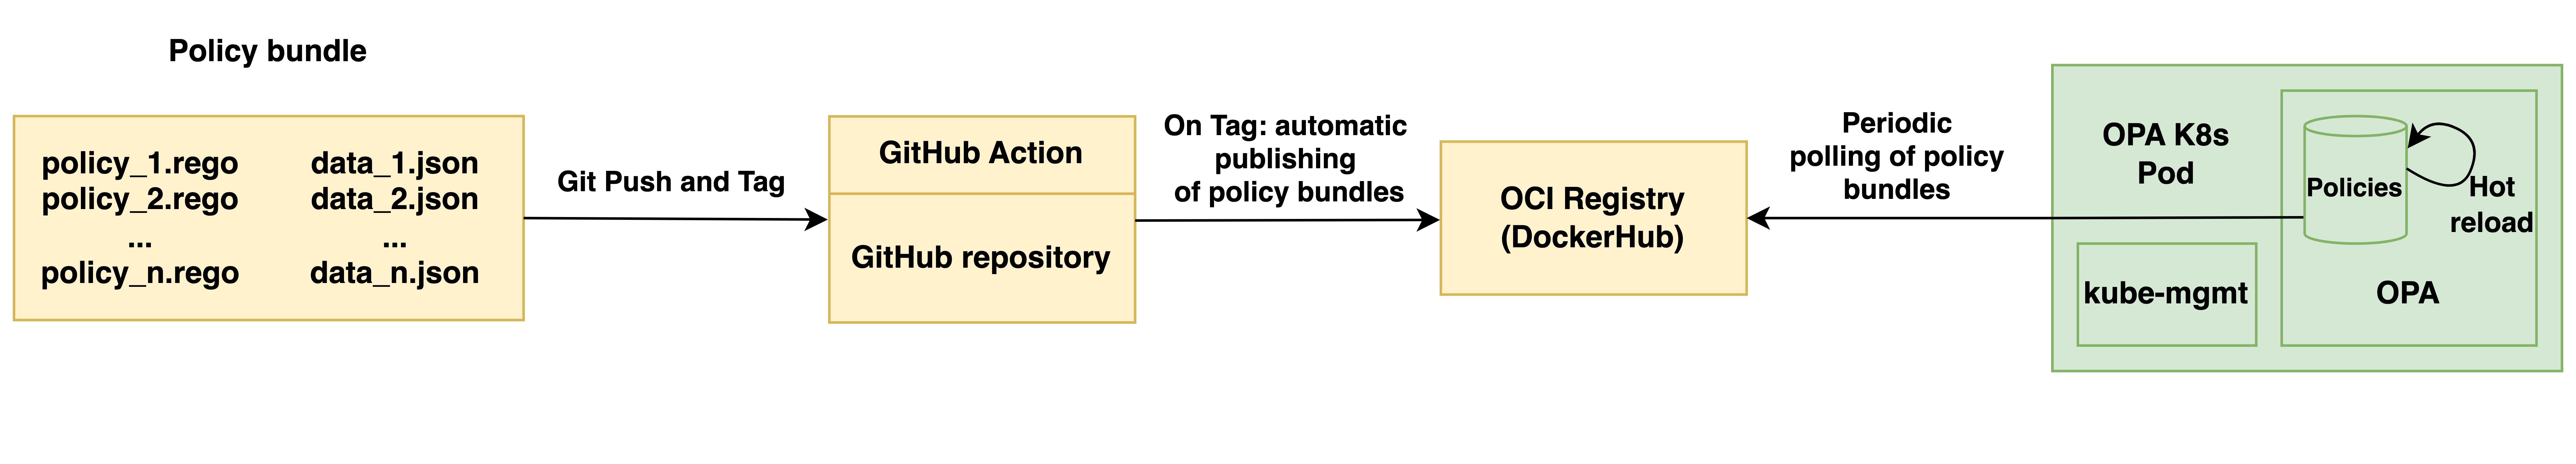
\includegraphics[width=1\linewidth]{images/opa_bundles.png}
\caption{OPA policy bundles}
\label{fig:opa_bundles}
\end{figure}

By leveraging OCI images for policy distribution and implementing a fully automated CI/CD pipeline, our system ensures that policy enforcement remains consistent, up to date, and highly available across all OPA instances. This approach aligns with modern DevOps practices, enabling organizations to maintain a high level of security and compliance without compromising operational efficiency.

\newpage

\subsection{OPA Gatekeeper}

OPA Gatekeeper is a Kubernetes-native policy engine that extends OPA with \textbf{Custom Resources (CRs)} and controllers to enforce policies across a Kubernetes cluster. It integrates natively with Kubernetes and provides a declarative approach to defining and enforcing policies using Kubernetes Custom Resources (CRs). This makes it an excellent choice for basic and standard policy enforcement scenarios, such as RBAC (Role-Based Access Control), security compliance, and resource constraints.
However, while OPA Gatekeeper is well-suited for simple use cases, it presents \textbf{limitations} when addressing complex policy requirements, particularly when policies involve \textbf{mutations} or require access to \textbf{external data sources}. These limitations make it unsuitable for the specific challenges tackled in this system. Therefore, after an initial investigation and Proof of Concept implementation, we decided to use the standard OPA server for policy enforcement mainly due to the flexibility it provides in handling diverse scenarios.

To illustrate the differences between a standard OPA policy and an OPA Gatekeeper policy, we present two examples:  
\begin{itemize}[itemsep=0.2pt, topsep=1pt]
  \item[$\bullet$] a simple Rego policy that enforces a basic constraint on Pod creation in a Kubernetes cluster.
  \item[$\bullet$] the corresponding policy implemented as an OPA Gatekeeper \textbf{ConstraintTemplate} and \textbf{Constraint} Kubernetes resources.
\end{itemize}

The first example demonstrates a standalone Rego policy, which can be evaluated directly by an OPA instance. While this approach is flexible and allows for fine-grained policy definition, it requires manual integration into the system, including policy distribution and enforcement setup.  

\lstset{style=python}
\begin{lstlisting}[language=rego, caption={Simple OPA Rego Policy}, label={lst:opa-rego}]
package kubernetes.admission

deny[msg] {
  input.request.kind.kind == "Pod"
  input.request.object.metadata.namespace == "restricted"
  msg := "Pods cannot be created in the 'restricted' namespace."
}
\end{lstlisting}

The second example, illustrated in listing \ref{lst:gatekeeper-template} utilizes OPA Gatekeeper, which extends OPA with Kubernetes-native Custom Resource Definitions (CRDs), enabling declarative policy management. By using a ConstraintTemplate, policies can be enforced dynamically through Kubernetes, making them easier to distribute and manage.
In other words, with this kind of setting, OPA policy bundles are not employed in the same way as in the standard OPA server. Instead, policies are defined as Kubernetes resources, allowing for more straightforward policy enforcement and management within a Kubernetes environment.

\begin{lstlisting}[language=yaml, caption={OPA Gatekeeper ConstraintTemplate}, label={lst:gatekeeper-template}]
apiVersion: templates.gatekeeper.sh/v1
kind: ConstraintTemplate
metadata:
  name: podnamespaceconstraint
spec:
  crd:
    spec:
      names:
        kind: PodNamespaceConstraint
  targets:
    - target: admission.k8s.gatekeeper.sh
      rego: |
        package kubernetes.admission
        deny[msg] {
          input.review.object.metadata.namespace == "restricted"
          msg := "Pods cannot be created in the 'restricted' namespace."
        }
\end{lstlisting}

\begin{lstlisting}[language=yaml, caption={OPA Gatekeeper Constraint}, label={lst:gatekeeper-constraint}]
apiVersion: constraints.gatekeeper.sh/v1beta1
kind: PodNamespaceConstraint
metadata:
  name: restrict-namespace
spec:
  match:
    kinds:
      - apiGroups: [""]
        kinds: ["Pod"]
  parameters: {}
\end{lstlisting}

In the example, the policy is defined as a ConstraintTemplate, which is then instantiated as a Constraint Custom Resource of kind defined in the ConstraintTemplate. The ConstraintTemplate specifies the Rego policy logic, while the Constraint defines the target resources and parameters for policy enforcement. Therefore a ConstraintTemplate can be used by multiple Constraints, allowing for policy reuse.

OPA Gatekeeper also provides additional Kubernetes Custom Resources called \textit{mutators} (Assign, AssignMetadata, AssignImage, ModifySet) that allow modifying resource fields without writing Rego code. These mutators are useful for simple transformations, such as setting default labels or annotations. However simultaneous mutation of multiple fields leveraging external data is not supported \cite{opa_gatekeeper_external_data}. This limitation, in the context of our system, determined the choice of the standard OPA server for policy enforcement.

It must be noted that OPA Gatekeeper limitations could be potentially addressed in future releases, making it a more viable option for complex policy enforcement scenarios. However, for the current system requirements, the standard OPA server was deemed more suitable due to its flexibility.

\subsection{Latency policy}

A representative example of a policy aligned with Service Level Objectives (SLOs) or Service Level Agreements (SLAs) is the latency policy described in this section.
Given an \textbf{origin region} and a \textbf{maximum latency threshold} (expressed in milliseconds), the objective is to determine a \textbf{set of eligible regions} where the inter-regional latency between the origin and each region in the set is equal to or below the specified threshold.
Enforcing such constraints helps mitigate the so-called ``\textbf{black hole phenomenon}" in the GreenOps use case, where all virtual machines (VMs) would otherwise be scheduled in a region with generally low carbon intensity, without considering additional constraints or performance requirements. By incorporating similar performance-aware policies, organizations can achieve a balance between environmental impact, performance, and service reliability.
The proposed flexible system enables organizations to fine-tune these factors according to their specific requirements or those of their users. 
This policy demonstrates the flexibility of OPA in handling diverse compliance scenarios. It is the responsibility of the policy developer to design an appropriate strategy for encoding relevant information into \textbf{well-structured JSON data models}, e.g., a latency matrix. Proper structuring ensures efficient policy evaluation, maintainability and extendability.

Figure \ref{fig:latency_matrix} illustrates an small example (4 regions subset) of a latency matrix, where each cell represents the latency between two regions. The matrix can be encoded in JSON format as illustrated in listing \ref{lst:latency_matrix_example}, allowing for easy integration with OPA policies. The ``Latency policy'' then uses this matrix to determine eligible regions based on the origin region and maximum latency threshold.

\begin{figure}[H]
  \centering
  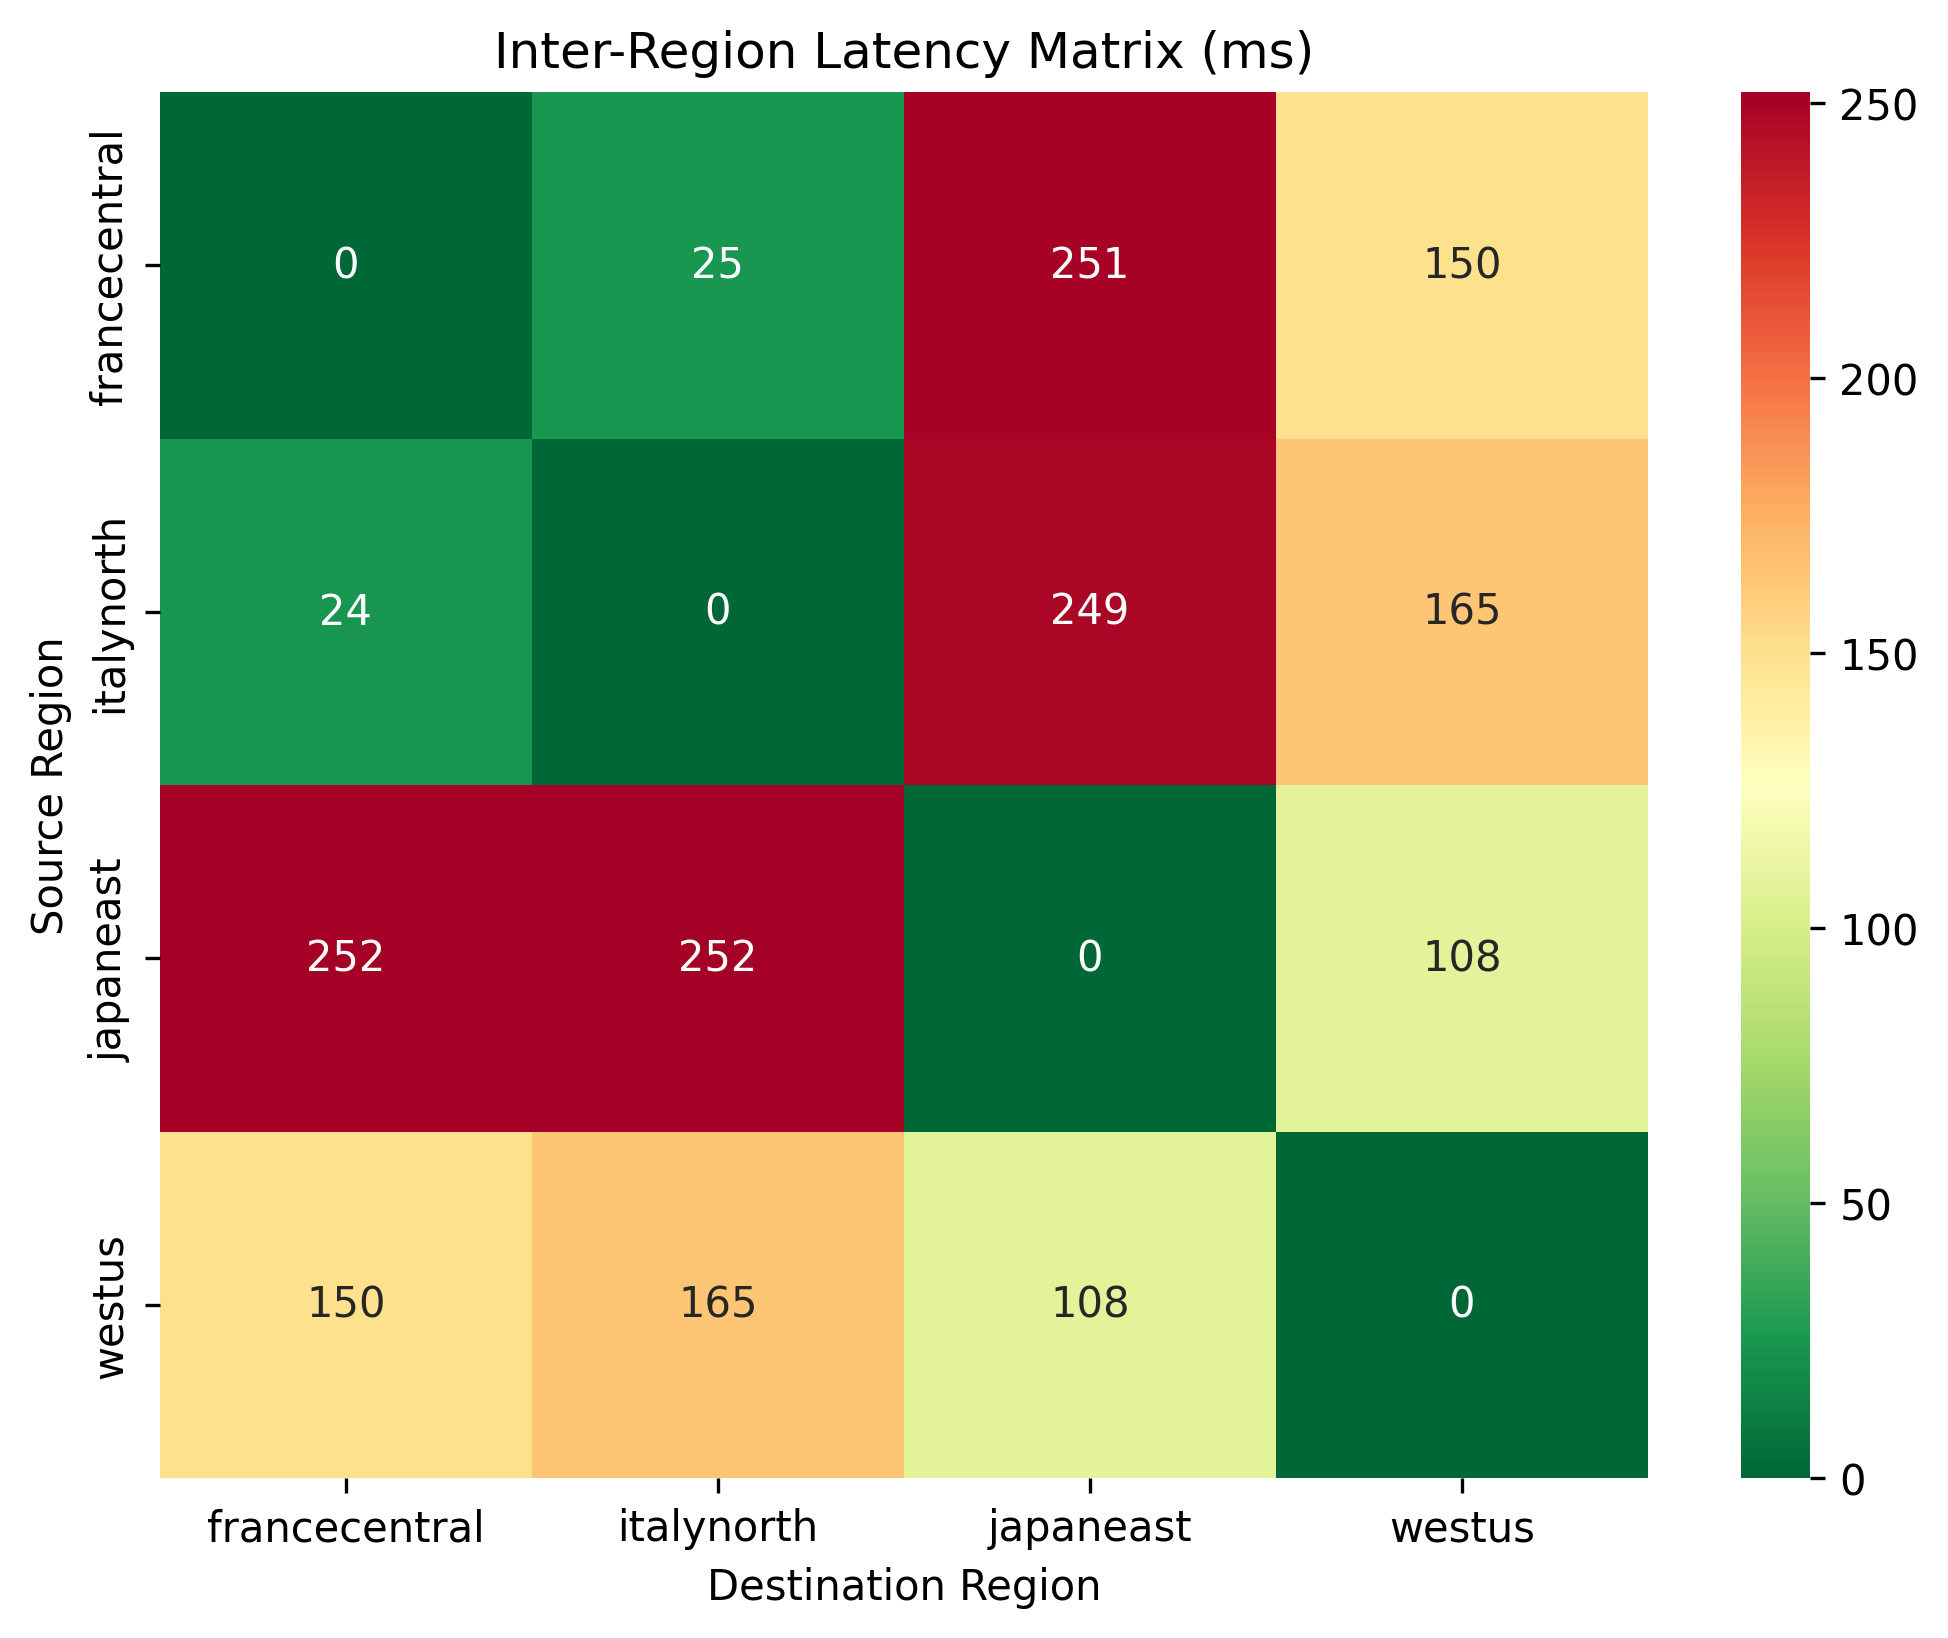
\includegraphics[width=0.75\linewidth]{images/latency_heatmap.png}
  \caption{Latency matrix example (Azure regions subset)}
  \label{fig:latency_matrix}
\end{figure}


\lstset{style=jsonstyle}
\begin{lstlisting}[caption={Latancy matrix example encoded in JSON format}, label={lst:latency_matrix_example}]
  {
    "italynorth": {
        "italynorth": 0,
        "japaneast": 249,
        "francecentral": 24,
        "westus": 165
    },
    "japaneast": {
        "italynorth": 252,
        "japaneast": 0,
        "francecentral": 252,
        "westus": 108
    },
    "francecentral": {
        "italynorth": 25,
        "japaneast": 251,
        "francecentral": 0,
        "westus": 150
    },
    "westus": {
        "italynorth": 165,
        "japaneast": 108,
        "francecentral": 150,
        "westus": 0
    }
}

\end{lstlisting}


data

Azure provides monthly Percentile P50 round trip times between Azure regions:
(https://learn.microsoft.com/en-us/azure/networking/azure-network-latency?tabs=Americas%2CWestUS)
https://learn.microsoft.com/en-us/azure/networking/media/azure-network-latency/azure-network-latency-thumb.png#lightbox 

Azure network latencies docs:
https://raw.githubusercontent.com/MicrosoftDocs/azure-docs/refs/heads/main/articles/networking/azure-network-latency.md

Merged Azure network latencies:
https://docs.google.com/spreadsheets/d/1kxtPw9ZSnAv1vQ6IDwzw-mXdHoKUFb8AjlsjACnvDqE/edit?usp=sharing 


AWS:
https://www.cloudping.co/grid (not official, not using VMs but Lambda functions)

google
syntetic data



\subsection{GDPR policy}

Another policy configured in the system is the ``GDPR Policy'', which ensures that virtual machines (VMs) are deployed in cloud regions that reside in countries of the European Union. 
The policy is based on the principle of \textbf{set intersection}. One set consists of the eligible regions determined by other constraints, such as latency requirements. The other set includes cloud provider regions that are physically located within European Union (EU) countries.
The intersection of these two sets defines the final list of allowed deployment regions, restricting workloads to EU-based data centers.
Since each cloud provider has its own regional distribution, the list of EU-compliant regions is provider-specific and is encoded as contextual data in JSON format. This allows for flexibility and easy updates when cloud providers introduce new regions.

It must be noted that this policy is \textbf{not intended to be a comprehensive GDPR compliance solution}, but rather a basic example of how OPA can enforce \textbf{data residency requirements in a multi-cloud environment}. Organizations with more stringent GDPR compliance needs should consider additional measures.

\subsection{Scheduling outcome policy}

main policy

Mutation policy
dedicated to 


JSON patch, what is a jsonpatch
patch code

encoded patches

\subsection{OPA Data mapping}

OPA is flexible enough to handle data mapping between different data models, enabling seamless integration with external systems. In our GreenOps system, data mapping is essential for translating between ElectricityMaps regions and cloud provider regions. 


At some point in the system this mapping needs to be done.
this mappings are needed since the scheudler knows only about ElectricityMaps regions, and do not possess the knowledge of cloud provider regions. Therefore, a mapping is needed to translate the ElectricityMaps regions to cloud provider regions and vice versa.

inside the policy is a good place to do this mapping


first filter is the selection of the provider
this determine the whole set of regions belonging to that provider

eligible regions: this filter can be only done with cloud provider specific latencies

\begin{figure}[H]
  \centering
  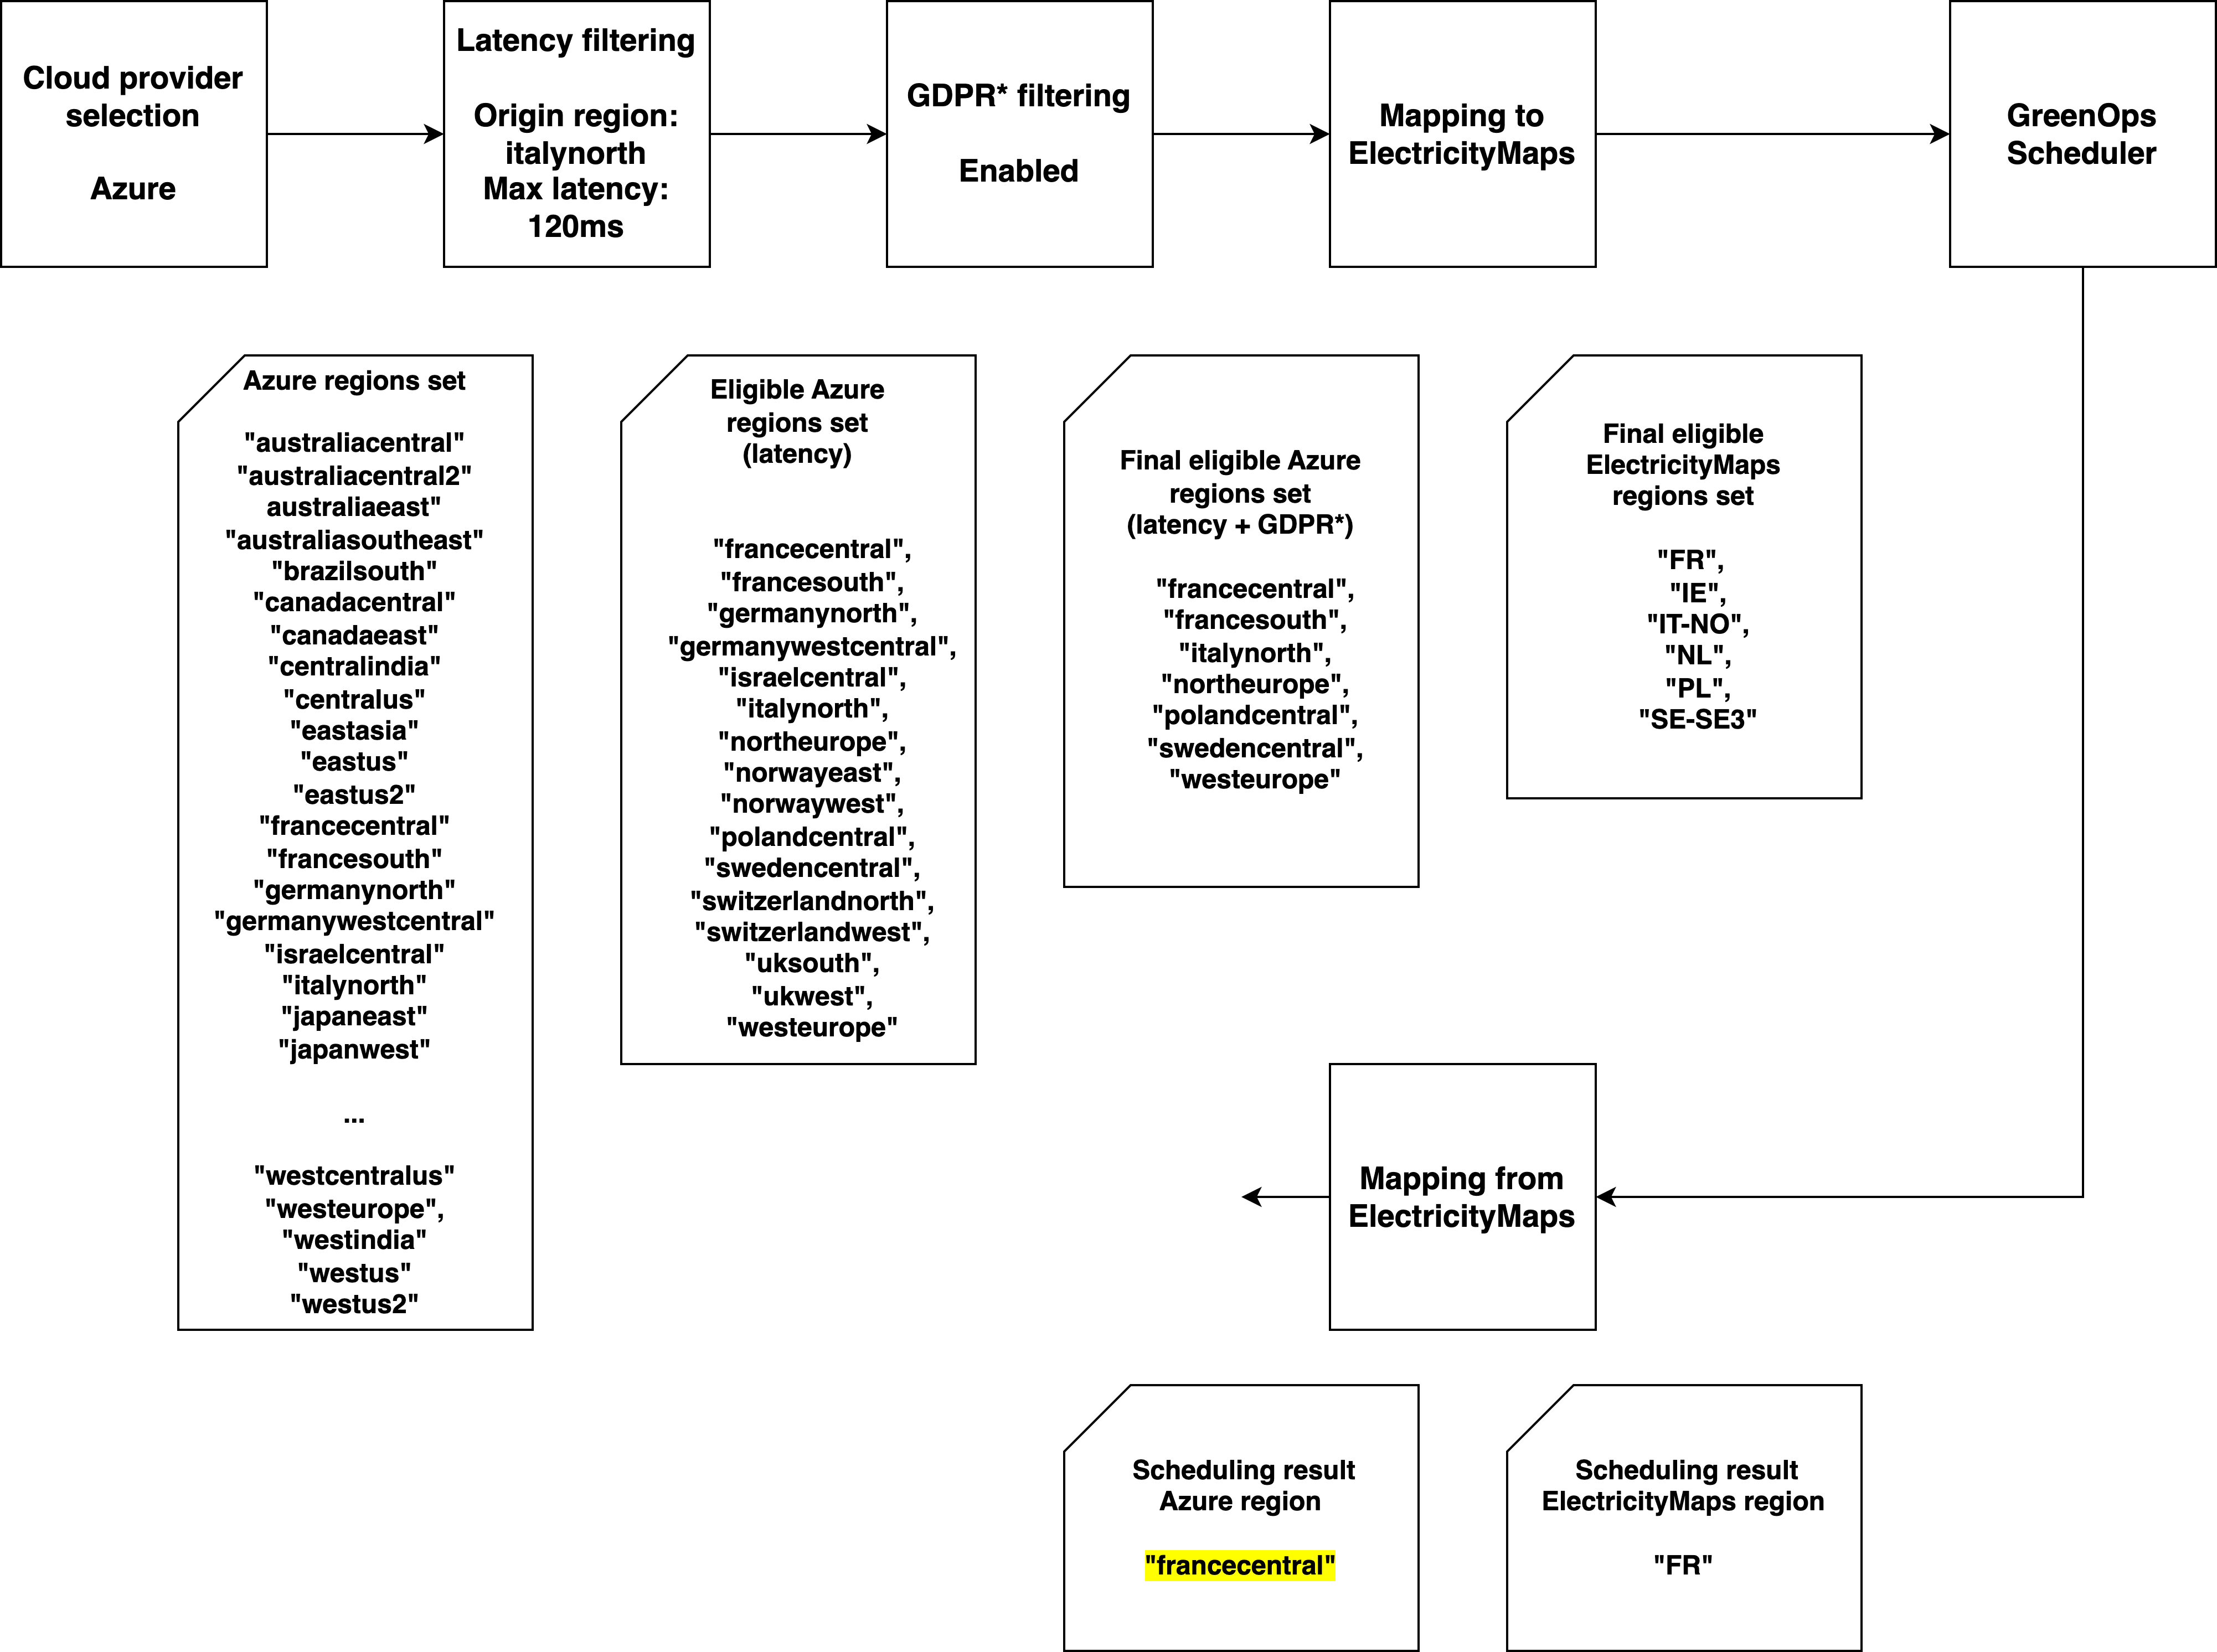
\includegraphics[width=1\linewidth]{images/data_mapping.png}
  \caption{OPA Data mapping}
  \label{fig:data_mapping}
\end{figure}


\begin{lstlisting}[language=Rego, caption=Rego data mapping, label=lst:rego_data_mapping]
# Utility functions to map between cloud provider regions 
# and ElectricityMaps regions

map_to_electricitymaps(eligible_regions, provider) = em_regions if {
    em_regions := {
        region.ElectricityMapsName |                             
        some eligible_region;                       
        some region;                                
        eligible_region = eligible_regions[_];      
        region = data[provider].cloud_regions[_];   
        region.Name == eligible_region             
        region.ElectricityMapsName != ""            
        region.ElectricityMapsName != "Unknown"
    }
}

map_from_electricitymaps(em_region, provider) = cloud_region if {
    some region;                              
    region = data[provider].cloud_regions[_];   
    region.ElectricityMapsName == em_region;    
    cloud_region := region.Name 
}

\end{lstlisting}

\subsection{OPA end-to-end workflow}

 (K8s mutating webhook)

OPA flow:

- admission review (contains max\_latency, origin\_region)

- policy contains cloud provider (or chose for the user)

- policy calculate subset of eligible regions

- policy will ask scheduling information to the scheduler (using http.send()










relationship with k8s mutating webhook

rego policies


scheduler has notions of 
electricity maps regions only

OPA is used also as a data mapping layer
both at request time
and at response time


\begin{figure}[htb]
\centering
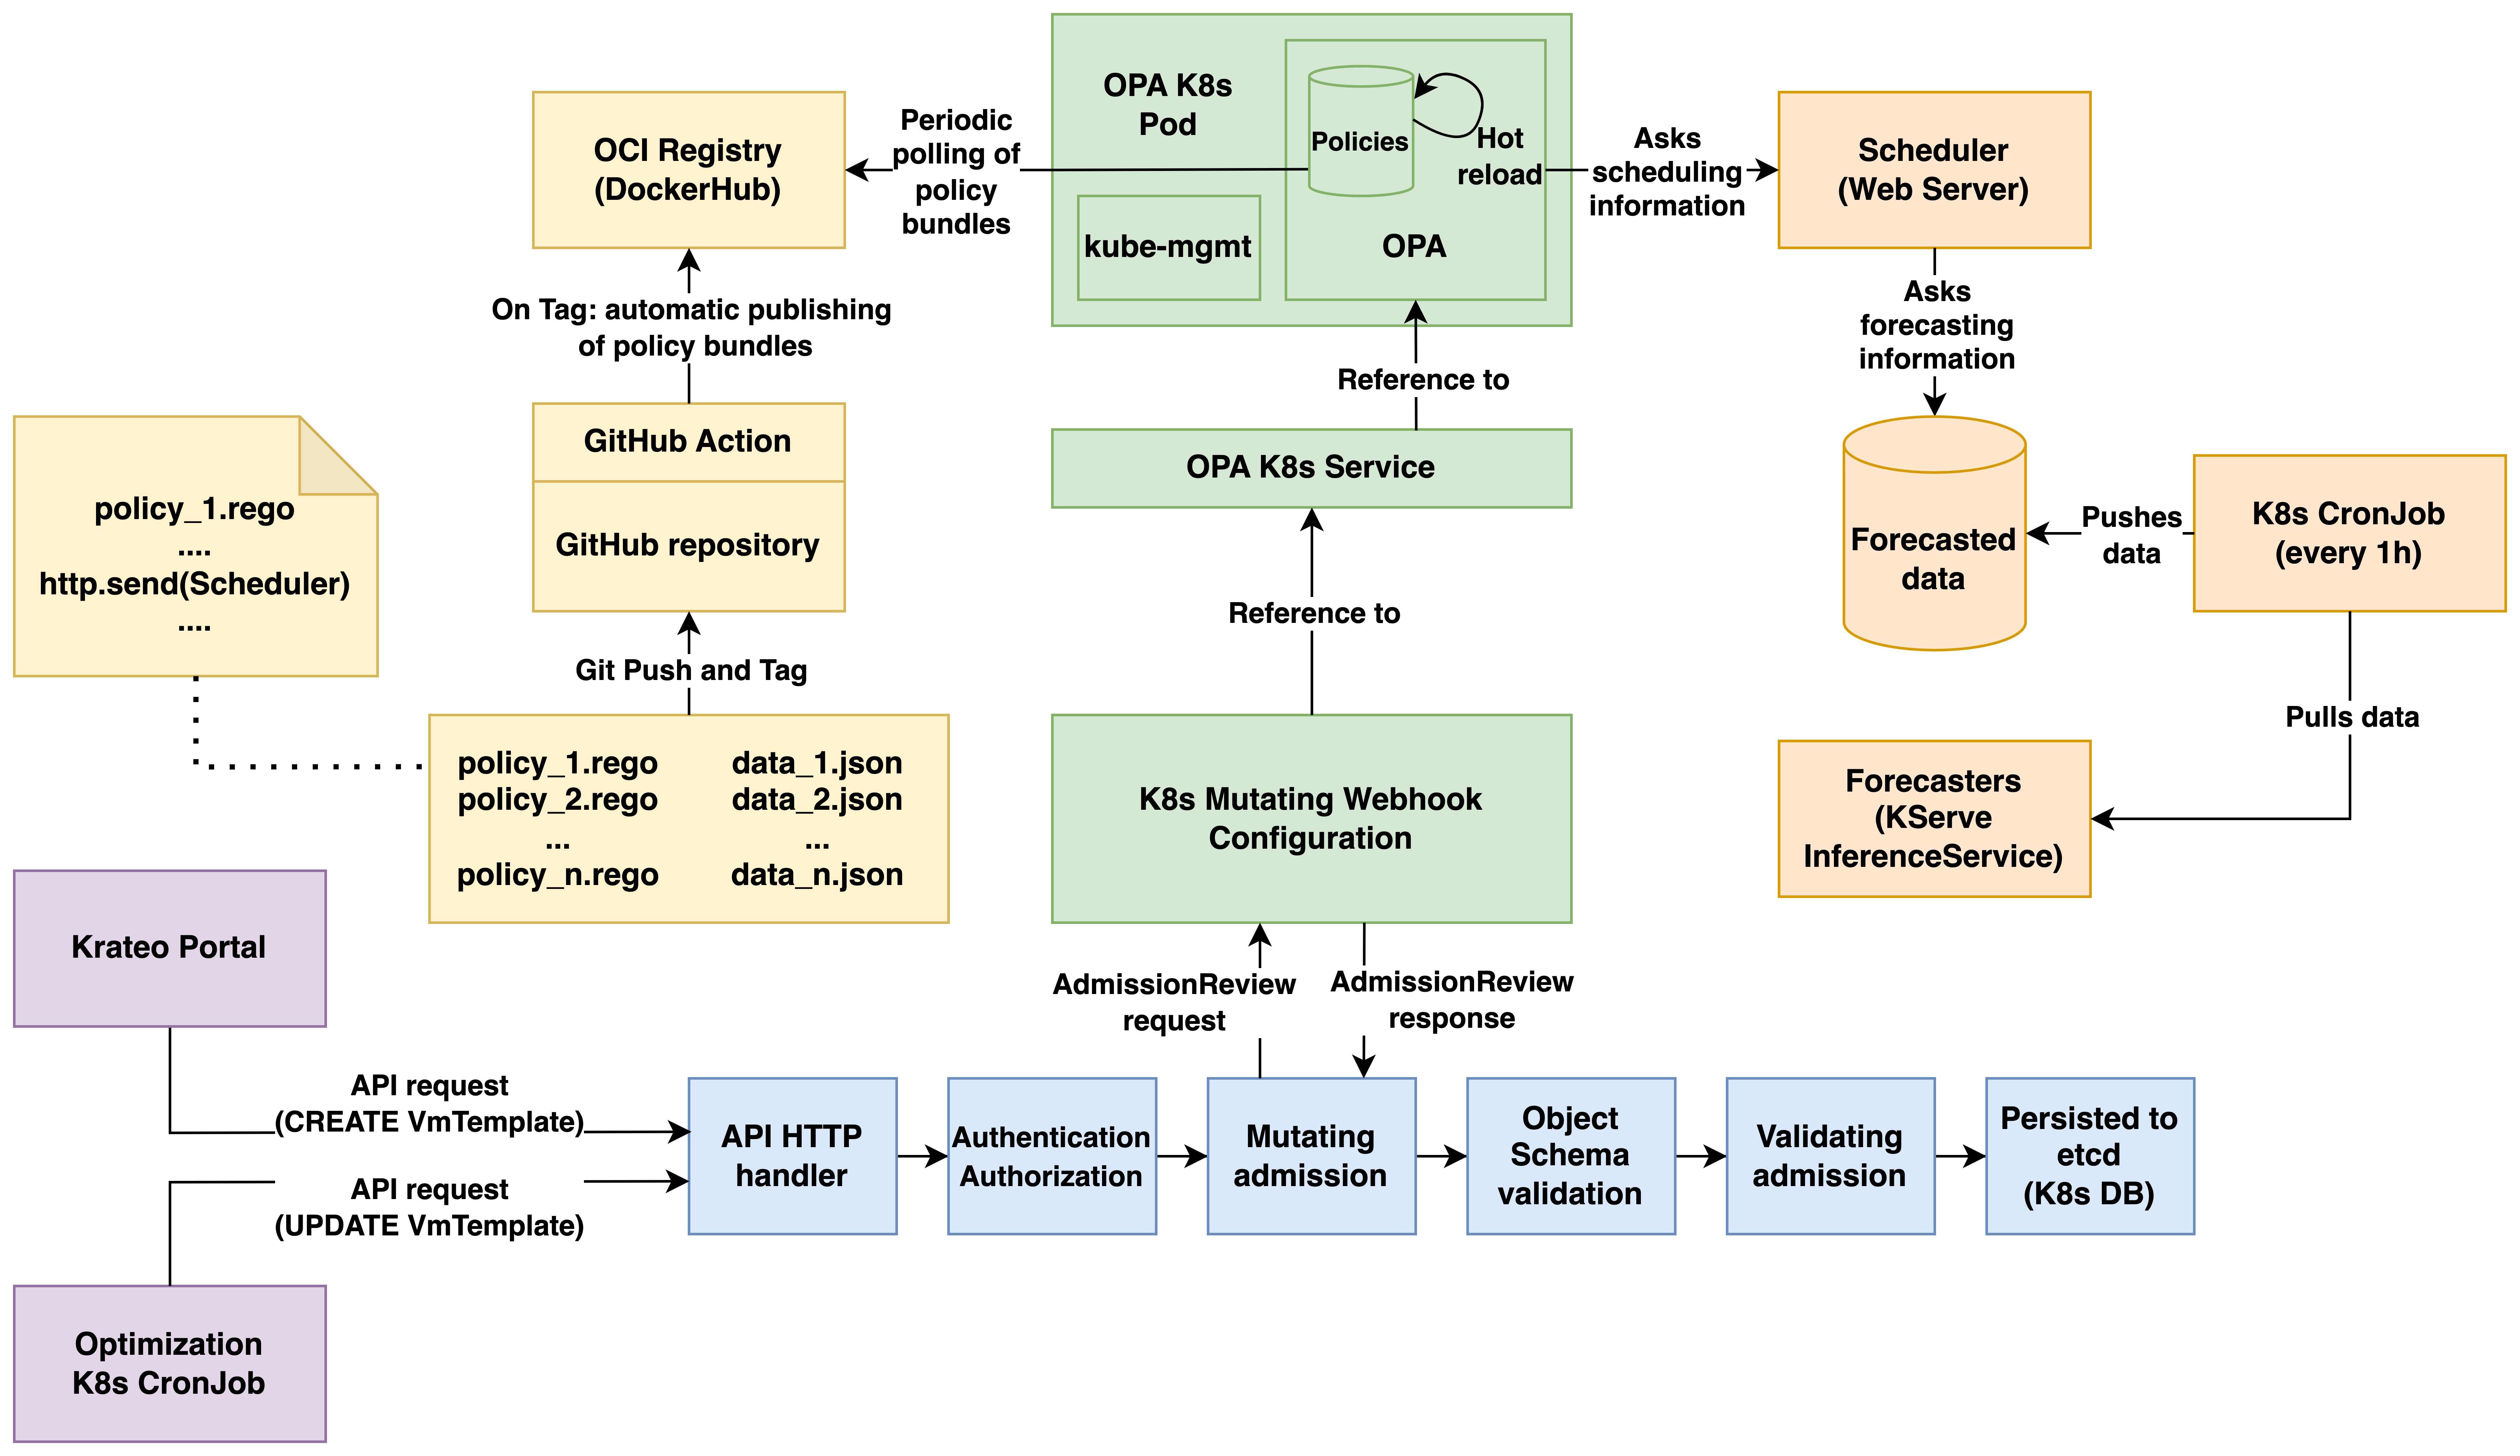
\includegraphics[width=1\linewidth]{images/mutating_webhook+OPA_integration.png}
\caption{Kubernetes mutating webhook + OPA integration}
\label{fig:webhook+opa}
\end{figure}

Figure \ref{fig:webhook+opa} represents the configuration of the Kubernetes Mutating Webhook with the intergeation of Open Policy Agent.
In particular, 




Day 2 operations
what are day 2 operations: in this case (VMs) resize a VM (scale up or down) based on the load
The mutating webhook configuration is set on the CREATE and UPDATE operations

UPDATE operation trigger
K8s Cronjob that attach a label to the custom resoruce 

\subsection{OPA advanced features}

It is deemed useful to mention some of the advanced features of OPA that were not employed in the system described in this thesis but could be potentially useful in future developments or in other contexts where OPA is used.

- bundle signing
- delta bundles

\newpage

\section{MLOps infrastructure}

A MLOps infrastrcutrue is not necessarily needed for multi-cloud resource management but since it is believed that ai or ml models will be used in the future more and more to get scheduling and management decisions, it is deemed important to describe a MLOps infrastructure in a Kubernetes environment.

\subsection{MLOps purpose}

MLOps implements DevOps principles, tools and practices into Machine Learning workflows 


purpose: industrialize ML models lifecycle

faster model development

faster model selection and deployment to production

\begin{itemize}[itemsep=0.2pt, topsep=1pt]
  \item[$\bullet$] model tracking (experiments, runs)
  \item[$\bullet$] model selection (model registry)
  \item[$\bullet$] model storage (in buckets)
  \item[$\bullet$] model deployment (inference)
\end{itemize}


allows all the team member to have visibility on the status of the ML models

Instead of having the so-called ``AI Inference Mock Server", treated as a black box returning a scheul;ding time and schedulingLocation

\begin{figure}[htb]
\centering
\includegraphics[width=1\linewidth]{images/mlops_workflow.png}
\caption{MLOps Architecture}
\label{fig:mlops}
\end{figure}


MLFlow framework

KServe framework


\subsection{MLflow}



MLflow Tracking Server


mlflow is compatible with many ML frameworks like sklearn, pythorch


what is a model tracking server
what is a model registry



Mlflow API calls
autolog function
infer signature 
important since store 

the end result is a self contained fodler with everythiong needed 
it allows reproducibility 

The training script will also serialise our trained model, leveraging the MLflow Model format.


model/
├── MLmodel
├── model.pkl
├── conda.yaml
└── requirements.tx


additional challenge: CrateDB is not supported natively by mlflow framework
a CrateDB adapter / wrapper is devoloped and mantianed by cratedb community
CrateDB as metadata stoere


SeaweedFS as artifact store
MINio could be an alternative altough it has a restrictive license \cite{minio_license}.



MODEL signature




\subsubsection{Alternative configuration 1}

watchdog
watchdog (pyhton package)
PoC
sidecar container

artifact store not needed

\subsubsection{Alternative configuration 2}

Another possible configuration could be the adoption of just CrateDB as both Metadata Store and Artifact Store.

This would be possible if
CrateDB supports blob storage but not object storage

This solution cannot be implemented yet




\subsection{KServe}


KServe Inference Service


what is
inference server / model server


used to deploy the forecaster (ML model)


uses Istio and Knative under the hood
but a deep descrption of those is out of the scope of this theses.
features: scaling to zero, etc


InferenceService with TorchServe runtime which is the default installed serving runtime for PyTorch models.

Kserve project proposes a standard protocol for inference servers.
The version 2 of the KServe Inference Protocol is the Open Inference Protocol.



\subsubsection{Open Inference Protocol}


\begin{table}[h!]
\centering
\begin{tabular}{|l|l|l|}
\hline
\textbf{API}    & \textbf{Verb} & \textbf{Path}                                                                                         \\ \hline
Inference       & POST          & v2/models/{[}/versions/\textless{}model\_version\textgreater{}{]}/infer                               \\ \hline
Model Ready     & GET           & v2/models/\textless{}model\_name\textgreater{}{[}/versions/{]}/ready                                  \\ \hline
Model Metadata  & GET           & v2/models/\textless{}model\_name\textgreater{}{[}/versions/\textless{}model\_version\textgreater{}{]} \\ \hline
Server Ready    & GET           & v2/health/ready                                                                                       \\ \hline
Server Live     & GET           & v2/health/live                                                                                        \\ \hline
Server Metadata & GET           & v2                                                                                                    \\ \hline
\end{tabular}
\end{table}





adopted by NVIDIA



multi model deployment



our strategy:
1 model per region
1 generic model? as fallback if specific model is not available?




Kserve "stack"

Kserve

in kserve 0.14.1
clusterservingruntimes
supported are 10
among which 
torchserve

clusterservingruntimes -> kserve-mlserver (supported models: sklearn, xgboost, lightgbm, mlflow)

mlserver

[chart to illustrate this]







serving runtimes

Seldon MLserver


accorgimenti: \\

\lstset{style=python}
\begin{lstlisting}[caption={Wrapping a PyTorch Model}, label={lst:wrapped_model}]
import torch

class WrappedModel(torch.nn.Module):
    def __init__(self, original_model):
        super().__init__()
        self.original_model = original_model

    def forward(self, *args, **kwargs):
        return self.original_model(*args, **kwargs)['prediction_outputs']

# Wrap the existing model
model = WrappedModel(model)

# Now calling model() will return only 'prediction_outputs' (test)
print(model(test_dataset[0]['past_values'].unsqueeze(0)))
\end{lstlisting}

\section{Measurements}


\subsection{System / performance metrics}


how to measuere cloud resource systems


especially useful for ``day 2 operations''
scaling down a VM


Metrics collected could be:
CPU usage
memory usage.
These metrics are especially useful for the 2nd use case for instance: scaling down a VM.


Prometheus exporters (https://prometheus.io/docs/instrumenting/exporters/) + Prometheus scrapers for data collection.
Generic Prometheus exporters and scrapers already used for Krateo Composable FinOps leveraging specific K8s Custom Resources. These exporters are generic and can scrape arbitrary metrics configured in specific CRs (for instance, collecting VMs CPU consumption though Azure APIs).
From the Krateo Composable FinOps document: 
- “we transform all optimizations into a set of Kubernetes Custom Resources (CRs) to act upon newly found cost-related deficiencies. This allows us to use Kubernetes operators (explicitly coded to interact with cloud services) to monitor these metrics and act automatically to apply changes to remote resources.”

- “forward the optimization to the Krateo operator that manages the services that need to be optimized, for example, the Azure Operator to modify the size of a Virtual Machine;”

- “the optimization is automatically encoded in a CR for the finops-operator-vm-manager, which then analyzes it and decides how to manage the Virtual Machine. For example, it could scale up or down the virtual machine, stop it for the night, etc.”

From my current understanding, only Azure is available for now on the finops-operator-vm-manager. 
This operator is only able to: start; stop; deallocate; scale-up; scale-down.
So finops-operator-vm-manager operates on already provisioned virtual machines and it applies optimizations.

---



Cloud providers API (“hypervisor” / host level) to get CPU usage, memory usage
Azure monitoring REST API: https://learn.microsoft.com/en-us/azure/azure-monitor/essentials/rest-api-walkthrough?tabs=rest%2Cportal
https://learn.microsoft.com/en-us/rest/api/monitor/metrics/list?view=rest-monitor-2023-10-01&tabs=HTTP
https://learn.microsoft.com/en-us/azure/virtual-machines/monitor-vm 


Cloud providers agents
Azure Monitor Agent (https://learn.microsoft.com/en-us/azure/azure-monitor/agents/azure-monitor-agent-overview)
Google Ops Agent: “the primary agent for collecting telemetry from your Compute Engine instances” (https://cloud.google.com/monitoring/agent/ops-agent)


Standard agents/deamons manually installed the VMs (e.g. Prometheus node exporter, 
many metrics restricted by public cloud providers
not straightforward to automate the deployment


---

Challenges
Public Cloud Providers do not provide data about carbon intensity of a VM instance
Public Cloud Providers do not provide data about power consumption of a VM instance

Power consumption metrics
scaphandre: NOT supported by public cloud providers. “Public cloud providers do not expose the underlying RAPL sensors that scaphandre and other measurement tools rely on to track consumption”. (https://github.com/hubblo-org/scaphandre/issues/142)
https://hubblo-org.github.io/scaphandre-documentation/index.html

kepler: really interesting and quite mature project but works only with K8s resources inside the cluster (Nodes, Pods). Therefore not good for our use first case.
https://sustainable-computing.io/design/architecture/


manually estimate power consumption based on CPU utilization, memory usage. Could be a very difficult task. 
there is the TEADS metodology like 



---


Carbon metrics:
there is no adopted standard, there is not something similar to FOCUS yet;
there is a proposal for a specification (work in progress, not supported yet by Public Cloud Providers): 
https://github.com/Green-Software-Foundation/real-time-cloud 
https://github.com/Green-Software-Foundation/real-time-cloud/blob/main/Cloud_Region_Metadata_specification.md 


Public Cloud Providers monthly reports (probably not useful in this case)
Export Azure carbon optimization emissions data (Preview) (probably not fine-grained as we want)

Cloud Carbon Footprint
Uses cloud provider billing (AWS Cost and Usage Reports with Amazon Athena, GCP Billing Export Table using BigQuery, Azure Consumption 
Management API). Using these services costs.
Electricity Maps API integration is supported (for live grid carbon intensity)

 
aether calculation engine (https://aether.green/docs/methodologies/) 
only AWS and GCP supported, Azure not yet
uses AWS CloudWatch and Google monitoring
very small project
no live Grid Carbon Intensity Coefficient, they extrapolate data from “governative” data reports
https://aether.green/docs/methodologies/#grid-carbon-intensity-coefficient


carbond agent) (https://gitlab.com/sustainable-computing-systems/carbond)
installed on the machine


Example of a manual approach (not scalable due to tech specs research): https://devblogs.microsoft.com/sustainable-software/how-can-i-calculate-co2eq-emissions-for-my-azure-vm/ 

The critical point here is to get/calculate the energy consumed by a cloud instance, since there are a huge number of technical configurations to find, retrieve and use for calculations.



\subsection{Impact framework}

Impact framework (by green software foundation)

\section{End-to-End workflow}
\label{sec:e2eflow}

[TO BE CHANGED]
A user request for a workload arrives in Kubernetes / Krateo. 
The request shape is VM1 = (MinCPU=4vCPU, MinRAM=4GiB, D=12h)
As we can see the request is generic: it does not contain a specific cloud provider or a specific cloud region.
A K8s Custom Resource (CR) representing the workload is created.
mutating webhook intercepts the CREATE API request.
K8s mutating webhook retrieve and evaluate policies and in particular, the AI model inference is called and should return a decision with the region and scheduling time (time-shifting and geographical shifting).
OPA will use this decision to mutate the VM specification, adding the provider, the schedulingRegion and schedulingTime fields.
Krateo core provider / cdc


\begin{sidewaysfigure}
  \centering
  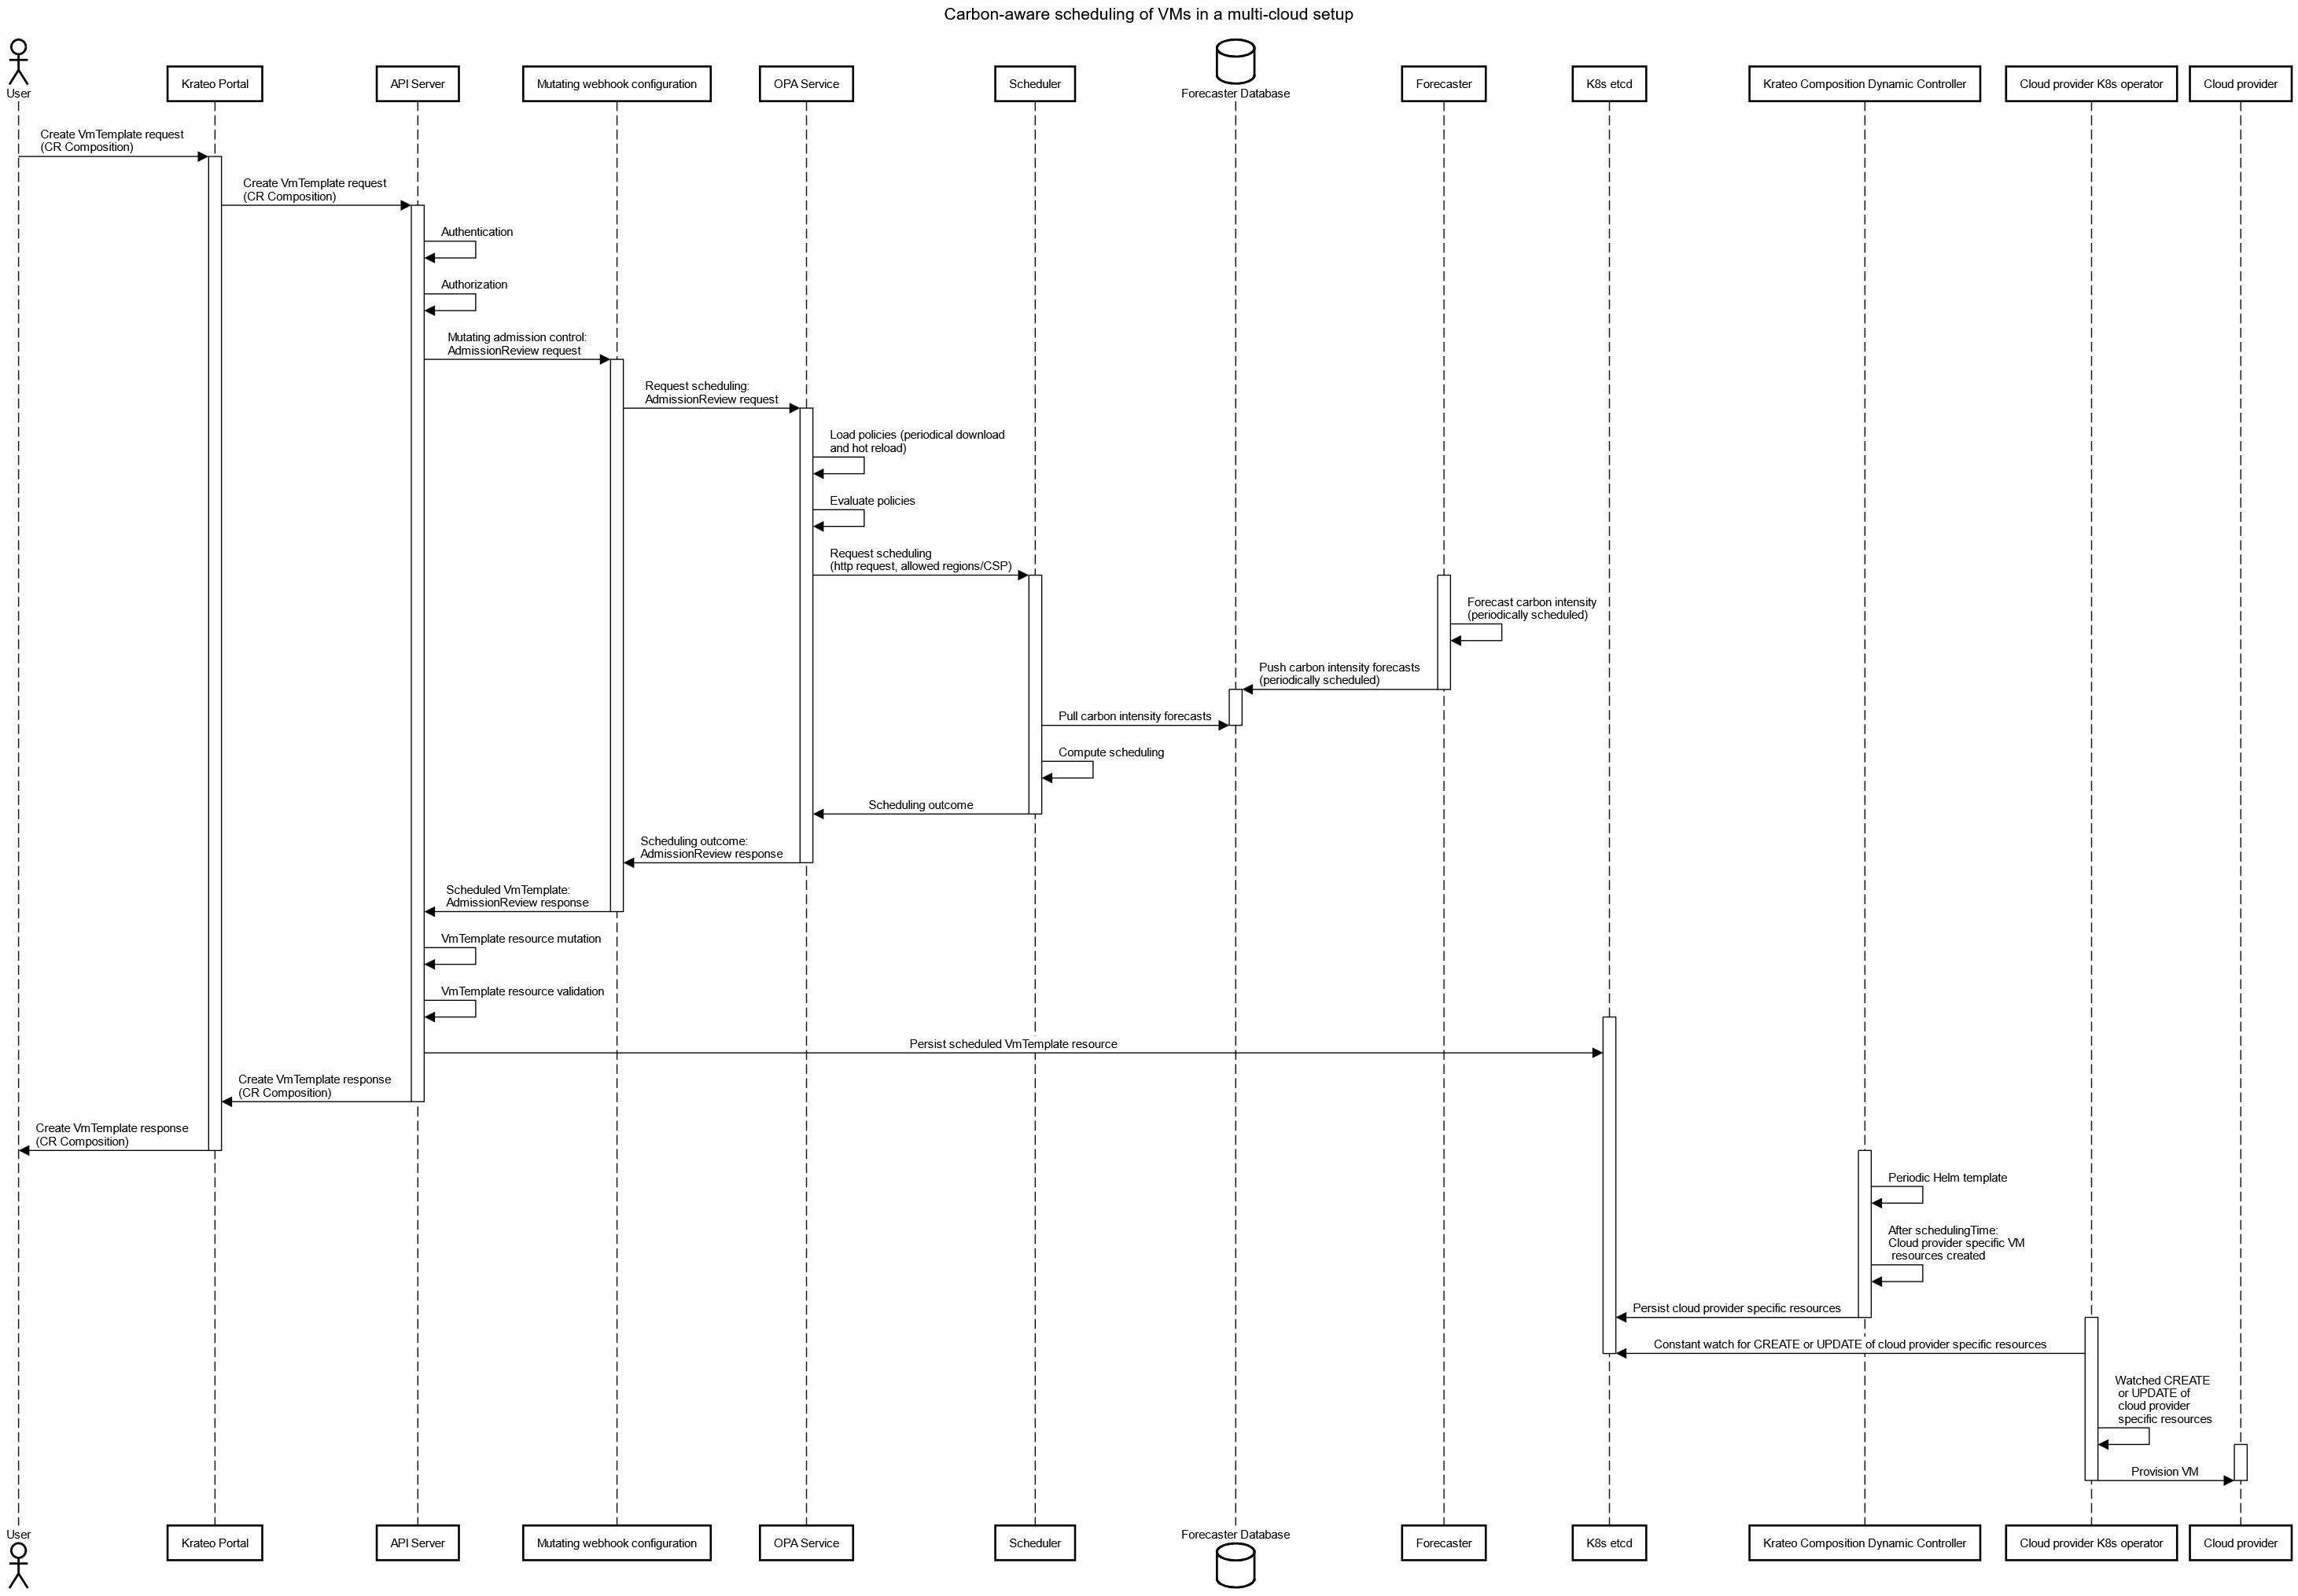
\includegraphics[width=\textheight]{images/sequence_diagram.png}
  \caption{Example of a full-page rotated image}
  \label{fig:rotated_image}
\end{sidewaysfigure}


\newpage







Table for recap of all tools used

Kubernetes
- Krateo
Helm
    Helm charts
    Helm templating
    Helm lookup function

- VmTemplate Krateo Composition Definition
- Azure K8s Operator
- GCP K8s Operator
- AWS K8s Operator
- K8s mutating webhook configuration
- OPA server
- opa policies
- OPA bundles
- MLflow tracking server (+ metadata store & artifact store)
- Forecaster (deployed as KServe InferenceService)


\newpage

      \chapter{Discussion}
\label{cha:discussion}

\section{End-to-end integrated test}

final result
A comprehensive end-to-end integrated test has been carried out on a Kubernetes cluster

this was used to validate the system

%(dependency graph)

\section{Theoretic upper bound}

 (how close can we get, masachussets amherest group)

\section{Baseline definition}

We should prepare one or more baseline schedulings that will be used as a baseline and compared with a carbon-aware scheduling proposed by our system.

\section{Black hole phenomenon}

How to deal with the so-called “Black hole” phenomenon?
That is, if 100 workload scheduling arrives at some point, there is the possibility that the outcome of the system we are building is: “schedule all workloads in Norway” where Norway is the region with least carbon intensity at that moment.
This phenomenon came up also in a previous meeting but it is not clear if this could be a problem etc..
A probable differentiator could be the max latency field of the workload request. Other service requirements could contribute to this as well.


(how it is countered)

\section{Side effects}

Maybe out of scope of this work, side effects, big picture.
What happens if a big percentage of companies that relies on cloud services starts to adopt carbon-aware scheduling of their workloads?
We tend to image cloud providers or even cloud regions as an infinite pool of resources, and at a certain level it is almost like that. But could carbon aware scheduling have larger, not foreseen, side effects?
Is this a responsibility of who schedules? Shall schedulers be responsible for the load on regions? Like self-imposing some sort of limits/caps. Ethics?

\section{Preliminary evaluation}

\begin{comment}
for the purpose of this theses

boavizta API simulation

assumptions
- analysis limited to only cloud VM, (aligned with the scope of this theses)
- data related to GCP is not data from boavizta (even if gcp is supported in our current system) but mapped from azure and aws

limitations
- whole countries, not regions


not easily integratable in a real production system due to its quite restrictive license (AGPL 3)
it is still usable for research purposes like in this case.
\end{comment}






\newpage

      \chapter{Conclusion}
\label{cha:conclusion}


production-ready system

\section{Future improvements}

day2 operations
we are ready for this

Scaling down a VM (example of Day 2 operations)
From: (4 vCPU, 8 GiB RAM)
To: (2 vCPU, 4 GiB RAM)

This use case is meaningful for workloads with durations in the order of at least days. Otherwise, for short-lived workload this use case does not make sense.
And in the case of workloads with days as duration, time and geographical shifting is not that relevant.

This use case will leverage system and performance metrics.








support for other resources
we need
templates
operators



there is one paper (https://ceur-ws.org/Vol-2382/ICT4S2019_paper_28.pdf) that uses local air temperature and solar irradiance as tiebreaker for 2 datacenters with similar carbon intense grid. 
“Local air temperature surrounding a datacentre affects the amount of energy needed for cooling”. 
They also claim that: “Solar irradiance varies more widely than carbon intensity across global regions”.

Maybe it could be an extension of our system in the future.


\subsection{Multi model serving}
"The original design of KServe deploys one model per InferenceService. But, when dealing with a large number of models, its 'one model, one server' paradigm presents challenges for a Kubernetes cluster."

kserve model mesh instead of several InferenceService
there is a lot of overhead in the current configuration

how much is better to use more models instead of one generic model 




\newpage


      
      
    \endgroup


    % bibliography - bibtex format
    %
    % add chapter to index
    \addcontentsline{toc}{chapter}{Bibliography}
    % alphabetical order of authors
    \bibliographystyle{plain}
    \bibliography{biblio}
%%%%%%%%%%%%%%%%%%%%%%%%%%%%%%%%%%%%%%%%%%%%%%%%%%%%%%%%%%%%%%%%%%%%%%%%%%
%%%%%%%%%%%%%%%%%%%%%%%%%%%%%%%%%%%%%%%%%%%%%%%%%%%%%%%%%%%%%%%%%%%%%%%%%%
%% Nota
%%%%%%%%%%%%%%%%%%%%%%%%%%%%%%%%%%%%%%%%%%%%%%%%%%%%%%%%%%%%%%%%%%%%%%%%%%
%% In the bibliography, all the sources consulted for the dissertation 
%% have to be cited and listed in alphabetical order by the 
%% first author's surname.
%%
%% According to the source material, the quotation has to be as follows:
%%
%% BOOKS
%% Surname and initial/s of the name/s of the author/s, date of edition,
%% publishing house and (if applicable) number of edition.
%% 
%% JOURNAL ARTICLES 
%% Surname and initial/s of the first name/s of the author/s,
%% title of the article, name of the journal, volume number, issue number
%% and page numbers.
%% 
%% CONFERENCE PAPERS
%% Surname and initial/s of the name/s of the author/s,
%% year of the conference, title of the article, name of the conference,
%% place of the conference, conference dates, page numbers.
%% 
%% CITING WEB RESOURCES
%% The consulted webpages have to be listed in alphabetical order. 
%% It is necessary to:
%%   - Copy the specific URL (the web address) of the consulted webpage
%%   - If available, indicate the surname and first name of the author/s,
%%     the title and subtitle of the text
%%   - If available, indicate the last date you retrieved the webpage
%%     (day/month/year).   
%%%%%%%%%%%%%%%%%%%%%%%%%%%%%%%%%%%%%%%%%%%%%%%%%%%%%%%%%%%%%%%%%%%%%%%%%%
%%%%%%%%%%%%%%%%%%%%%%%%%%%%%%%%%%%%%%%%%%%%%%%%%%%%%%%%%%%%%%%%%%%%%%%%%%
    

    \titleformat{\chapter}
        {\normalfont\Huge\bfseries}{Appendix \thechapter}{1em}{}
    % Appendix / attachment section - optional
    %\appendix
    %\chapter{Title first appendix}

test

\section{Title}
test

\subsection{Sub-title}
test


\chapter{Title second appendix}

test

\section{Title}
test 

\subsection{Sub-title}






\end{document}
